% Source update: Born--Hopf Framework v3.053 -- integrated graph closures with v3.041 Newton rebase.
% Paper-series v2.382: audit-identified standalone repair integration; mathematical scopes and open physical owners preserved.
% Paper-series v2.381: complete algebraic exceptional torsion atlas and all-cocycle twist-stability; original claims retained.
% Paper-series v2.380: unified bibliography, exact exceptional double/length/gauge mathematics in I-B; previous theorem labels retained.
% Paper-series v2.379: full equivariant Dirac/Hodge/eta/torsion atlas in Paper I-B; paper-root references synchronized.
% Paper-series v2.378: 2026 exceptional literature consolidation and reference synchronization. The mathematical additions are located in Paper I-B.
% Paper-series v2.377: reference-only rebind to current Paper I-B v1.1; original mathematics retained except new Paper I-B comparison chapter.
% Framework v2.370: derived exceptional-root/Hurwitz comparison in I-A/I-C; other papers reference-only synchronized.
% Framework v2.368: preserve prior II-B convention/unital fixes and verified II-D corrections; current references synchronized.
% Framework v2.358: current 30-root source reference synchronization; selectively updated III-E, III-F, VI-B, VI-C.
% Framework v2.356: bibliography/source-registry synchronization; mathematical body unchanged.
% Framework v2.353: conditional Dirac boundary-Schur source certificates; native action still open.
% Cumulative Petersen--Hopf Paper VI update v2.322: finite harmonic lift and conditional physical readouts.
% Framework v2.275: exact positive dense-twin word cubature, finite repeatability and eighth-moment classification, nested sampling frames, joint action and POVM-jet exports; preserves v2.274.
% Framework v2.274: two-scalar positive convolution certificates, first-leaked exceptional coset detection, branch-symmetric twin mixing, and finite endpoint moments; all v2.273 branches preserved.
% Framework v2.273: restored missing Problem 3 theorems from v2.268; exact exceptional frames, twin geometry, convolution repeatability and projector/occurrence firewalls; merged on v2.272 without overwriting independent branches.
% Framework v2.272: merged v2.270 covariant native-readout mathematics with v2.271 Problem 4 finite-action Hopf hypercharge/holonomy corrections; no universal bulk-gauge uniqueness claim.
% Independent branches: v2.270 readout/guard exports and v2.270 K16 action-consumed charge closure; all prior scoped assumptions retained.
% Framework v2.267: exact Paper II-A converse/observable certificates, III-F action tests, V-B right orbit and V-C native gauge scope; prior v2.266 preserved.
% Framework v2.266: exact Paper II-C outcome-count/readout converse results and scoped downstream imports; 30-root references synchronized.
% Framework v2.265: II-C coordinate-stage constitution and exact first-symbol host inheritance; prior mathematical domains retained.
% Framework v2.264: II-B reverse and action-bridge integration; preserves prior mathematical domains; active 30-root references synchronized.
% Framework v2.263: Paper I-D adds bridge-controlled root-carry parity and source-relative old-cap cancellation; other root mathematical bodies retained; active 30-root references synchronized.
% Framework v2.262: merges Paper II-F three-gap closure from v2.260 into v2.261, preserving newer II-B/II-D repairs; 30-root references synchronized.
% Framework v2.261: merged Paper II-B GP2-level/geometric repairs; preserves v2.260 II-D repairs; active references synchronized.
% Framework v2.260: Paper II-D signed RS, finite-symbol typing, and conditional curvature/Jordan repairs; references synchronized.
% Framework v2.259: conditional native SU(2) atlas and explicit later discharge; v2.258 mathematical bodies retained elsewhere.
% Framework v2.258: preserves parallel II-A/dynamics update and adds complete readout/frequency closures.
% Framework v2.257: exact minimal complete position readout and arbitrary-preparation frequency law.
% Framework v2.256: exact native inertia and sharp bounded ordered-source closure; preserves concurrent v2.255 work.
% Framework v2.255: preserves parallel detector integration and adds exact finite readout closures.
% Framework v2.254: shared bibliography/reference sync; substantive Pasterski detector-Ward additions only IV-B/IV-C/VII-C.
% Framework v2.253: typed raw coordinate defect in I-A and synchronized VI-A import; active references synchronized.
% Framework v2.252: optional shell-frame source-return calculation in III-G; active references synchronized.
% Framework v2.251: forward common-action execution, joint source jets and scoped coupled control.
% Framework v2.251: exact full-heat variations, fermion source jets and explicit physical completion frontier.
% Framework v2.251: certified interacting source jets, pole stability and scoped completion proofs.
% Framework v2.251: interacting finite-source evaluation and coupled local vacuum classification.
% Framework v2.251: exact finite source execution and native causal common-parent bridge.
% Framework v2.251: constructive parent and scoped source-incidence audit; see release report.
% Framework v2.251: common-action two-jet, corrected source/response closure and synchronized references.
% Framework v2.244: scoped rooted source-order Schur diagnostics and synchronized paper references.
% Framework v2.242: signed rooted phase lift, complete transverse return and exact family cubic.
% Framework v2.241: proved rooted conormal geometry, conditional cap realization and scoped action tests.
% Framework v2.239: coherent 30-paper reference rebinding; selective new proofs on established owners.
\documentclass[12pt,a4paper]{article}
\usepackage{graphicx}
\usepackage{float}
\usepackage{tikz}
\usepackage{tikz-cd}
\usepackage{microtype}
\usepackage{parskip}
\usepackage{caption}
\usepackage{subcaption}
\usepackage{slashed}
\usepackage{pgfplots}
\usepackage{makecell}
\usepackage{listings}
\usepackage{xltabular}
\usepackage{mathrsfs}
\usepackage{mathtools}
\usepgfplotslibrary{groupplots,fillbetween}
\pgfplotsset{compat=1.18}
\usetikzlibrary{shapes.geometric,arrows,positioning,shadows,intersections,plotmarks,decorations.pathreplacing}
% Macros-v2_188: re-based current paper identities and A--G family; no change to geometry.
% Macros-v2_184: active Paper III-E v1.200/III-F v1.267 binding for framework v3.031; mathematical macros unchanged.
% Macros-v2_183: updated shared cross-reference bindings for Paper1B/III-E/III-F v3.030; mathematical macros unchanged.
% Macros-v2_182: active Paper II-F/V-A cross-references for framework v3.029; definitions unchanged.
% Paper-series v2.381: new I-B torsion/modular results, bibliography and current source roots.
% Paper-series v2.380: new exceptional bibliography and synchronized paper references.
% Paper-series v2.379 current 31-paper macro/aux registry.
% Paper-series v2.378: current 31-paper AUX/bibliography registry updated for Paper I-B v1.2 literature additions.
% Framework v2.371: current-source reference registry refreshed; old theorem labels retained.
% Framework v2.370: current 30-paper source/AUX root rebinding; native mathematical macros unchanged.
% Framework v2.368: synchronized merged 30-root registry; mathematical notation unchanged.
% Framework v2.358: active 30-paper source registry synchronized; existing mathematical macros unchanged.
% Framework v2.357: selective new source-owned certificates; active reference roots updated for five revised papers.
% Framework v2.356: active 30-root registry synchronized to the 30 papers in this release.
% Framework v2.275: exact positive dense-twin word cubature, finite repeatability and eighth-moment classification, nested sampling frames, joint action and POVM-jet exports; preserves v2.274.
% Framework v2.274: filename and root-source synchronization.
% Framework v2.273: restored missing Problem 3 theorems from v2.268; exact exceptional frames, twin geometry, convolution repeatability and projector/occurrence firewalls; merged on v2.272 without overwriting independent branches.
% Framework v2.272: merged v2.270 covariant native-readout mathematics with v2.271 Problem 4 finite-action Hopf hypercharge/holonomy corrections; no universal bulk-gauge uniqueness claim.
% Independent branches: v2.270 readout/guard exports and v2.270 K16 action-consumed charge closure; all prior scoped assumptions retained.
% Framework v2.269: synchronized 30 active AUX roots; mathematics and bibliography preserved from Macros-v2_161.
% Framework v2.266: Paper II-C converse-derived outcome resources; II-E, III-C, IV-A/B, V-A and VI-B downstream mathematical closures; 30-root registry synchronized.
% Framework v2.265: II-C coordinate-stage constitution and exact first-symbol host inheritance; prior mathematical domains retained.
% Framework v2.264: paper II-B reverse/audit and IV-A observable-minimal exchange; synchronized external references to 30 active roots.
% Framework v2.263: Paper I-C adds bridge-controlled root-carry parity and source-relative old-cap cancellation; other root mathematical bodies retained; active 30-root references synchronized.
% Framework v2.262: integrates Paper II-F radius, Casimir and readout results; active 30-root references synchronized.
% Framework v2.261: merged Paper II-B GP2-level/geometric repairs; preserves v2.260 II-D repairs; active references synchronized.
% Framework v2.260: Paper II-D signed RS, finite-symbol typing, and conditional curvature/Jordan repairs; references synchronized.
% Framework v2.259: conditional native SU(2) atlas and explicit later discharge; v2.258 mathematical bodies retained elsewhere.
% Framework v2.258: preserves parallel II-A/dynamics update and adds complete readout/frequency closures.
% Framework v2.257: exact minimal complete position readout and arbitrary-preparation frequency law.
% Framework v2.256: exact native inertia and sharp bounded ordered-source closure; preserves concurrent v2.255 work.
% Framework v2.255: preserves parallel detector integration and adds exact finite readout closures.
% Framework v2.254: Pasterski bibliography and synchronized 30-paper external-reference registry.
% Framework v2.253: typed raw coordinate defect in I-A and synchronized VI-A import; active references synchronized.
% Framework v2.252: synchronized source registry; optional III-G shell-frame calculation.
% Framework v2.251: forward common-action execution, joint source jets and scoped coupled control.
% Framework v2.251: exact full-heat variations, fermion source jets and explicit physical completion frontier.
% Framework v2.251: certified interacting source jets, pole stability and scoped completion proofs.
% Framework v2.251: synchronized active source registry; mathematical notation unchanged.
% Framework v2.251: synchronized active source registry; mathematical notation unchanged.
% Framework v2.251: synchronized active source registry; mathematical notation unchanged.
% Framework v2.251: synchronized source registry; no mathematical notation changes.
% Framework v2.244: synchronized 30-paper AUX registry and rooted phase-source action-order tests.
% Framework v2.242: signed rooted phase lift, complete transverse return and exact family cubic.
% Framework v2.241: proved rooted conormal geometry, conditional cap realization and scoped action tests.
% Framework v2.239: all 30 active source roots synchronized; no mathematical macro changes.
% Framework v2.238: Paper IV A/B/C split and 30-root reference registry.
% Framework v2.237: Paper VII-D technical split and 28-root reference registry.
% Framework v2.236: Paper VI-C technical-volume reference added; all current root bindings advanced.
% Framework v2.235: 26-root AUX and bibliography bindings synchronized; mathematical macros unchanged.
% BEGIN INLINE SOURCE: Paper00-TeXBuildCompatibility-v1_0.tex
% Rendering-only repairs for inherited long appendices and bitmap text fonts.
% Integer counters through 26 retain the original labels; later values use AA,
% AB, ... . This file changes no action coefficient, state or theorem premise.
\RequirePackage{alphalph}
\makeatletter
\let\BHPrimitiveAlph\@Alph
\newalphalph{\BHExtendedAlph}{\BHPrimitiveAlph}{26}
\let\@Alph\BHExtendedAlph
\AtBeginDocument{%
  \@ifpackageloaded{microtype}{\microtypesetup{expansion=false}}{}%
}
\makeatother

% END INLINE SOURCE: Paper00-TeXBuildCompatibility-v1_0.tex

% Framework v2.164: current reference/bibliography profile; mathematical definitions retained.
% Framework v2.162: finite metric, functional Hilbert and scoped Ward integration.
% Framework v2.161: inherits Macros-v2_57.tex exactly except the current external-reference binding.
% Macros v2.57 / framework v2.156: current reference registry only; mathematical definitions unchanged.
% Framework v2.143 / Macros v2.55: current external-reference bindings; mathematical notation unchanged.
% Framework v2.110 / Macros v2.54: current external-reference registry and bibliography; mathematical notation inherited.
% Framework v2.67 / Macros-v2_53: adds Born-action-cell and joint-EH readout symbols; absolute unit realization is metrological; MATCH_{J/scal}^{EH} remains the sole G24 normalization bridge.
% Framework v2.35 / Macros-v2_52: grouped paper numbering, active AUX registry, and Born-v6_20 bibliography binding synchronized; notation unchanged.
% Framework v2.26: active-source AUX and bibliography bindings synchronized; notation unchanged.
% Framework v2.09: reviewed early-reciprocity integration; scoped physical imports.
% Framework v2.08: Born--Euler mathematics and conditional complete-action potential criterion.
% Framework v2.07: active AUX registry includes Paper I-B v1.2; shared bibliography Born-v6_18.
% Macros-v2_46 / framework v2.04: mathematical atlas and downstream realization correction.
% Macros-v2_46 / framework v2.03: scoped structure integration and current dependency bindings.
% Macros-v2_46 / framework v2.01: shared source bindings; prior revision comments are historical.
% v2.42 / framework v1.99: Synchronized RG/AS owner and bibliography bindings.
% v2.41 / framework v1.99: active manuscript AUX bindings and geometric-closure bibliography synchronized.
% Release-v1.80 centralized source synchronization for scalar-circle/comparison-band integration.
% Release v1.79: Hurwitz hierarchy and kinetic-normalized action response integration; physical mass matching remains conditional.
% Release v1.78: approved M8 closure-batch integration; physical and analytic domains retained.
% Current v1.78 registry: all active TeX roots are synchronized below.
% Earlier release comments are historical scope records, not current status.
% Release-v1.77 synchronization: native same-owner Noether closure, generator--flow/history typing, analytic-certification firewalls, scalaron/K16, LF/QCD, quantum-Ward, and RAR boundary-owner transport are registered; shared mathematical notation is unchanged.
% Release-v1.76 synchronization: registry points to the v1.76 active paper roots.
% Release-v1.76 synchronization: registers the local A+Phi+g Noether/constraint closure and dynamics-frontier propagation; shared mathematical notation is unchanged.
% Release-v1.75 synchronization: registry points to the v1.75 active paper roots.
% Release-v1.75 synchronization: integrates the joint-Dirac Einstein bulk real form and the local odd-scalar heat-coefficient action on explicit analytic first-jet/interior domains; v1.74 Yang--Mills closure is retained. Fermionic reality, pure-metric curvature-squared/exact-nonlocal terms, noncanonical boundaries, physical vacuum selection, and actual solution-history tokens remain open.
% Release-v1.74 synchronization: registry points to the v1.74 active paper roots and retains the v1.73 theorem labels.
% Release-v1.74 synchronization: canonical Macros-v2_34.tex; generated local nonlinear Yang--Mills action, constrained connection-field phase space, source-free Gauss momentum map, and Legendre closure are integrated on their proved domains. The remaining non-gauge ACT_cl sectors and actual solution-history selection remain open.
% Release-v1.71 synchronization: closes the former JOINT_x/JOINT_5
% connection-occurrence gap by canonical structure-group extension of the
% nonflat Born connection, faithful associated representation, and the local
% cotangent--Clifford operator constructor.  Actual fluctuation members,
% actions, vacua, solutions, calibrations, and analytic QFT domains remain
% separately typed.  The active-AUX registry is advanced once.
% Release-v1.71 canonical macro and active-AUX registry.
% ======================================================================
% Macros-v2_39.tex -- canonical publication macro file
% Release v1.71 retains the v1.70 null-ray/QCD boundaries and additionally
% removes the duplicate structural connection actuality premise.  It does not
% claim global bundle topology, select a gauge/Higgs member, or promote the
% finite construction to an interacting continuum theory.
% Release v1.68 constructs the finite light-front total-fraction operators and
% parton number/momentum operator measures, proves their simplex and Hausdorff-limit
% theorems, and separates positive cut measures from scheme-renormalized
% light-ray distributions.  It also separates finite real Schur poles, stable
% norm-resolvent/Riesz pole-residue limits, and continued resonance
% pole/residue limits.  The Paper-VII-C scattering package is claim-indexed:
% local QFT and spectral claims import no S-matrix or infrared premise, while
% asymptotic amplitudes, LSZ, S-matrix poles, completeness, and cross sections
% import only their named massive or massless/long-range clauses.
% Release v1.67 factorizes BND48_H into a same-action Hessian/Schur
% descendant and still-open typed boundary-trace, critical-lift, and
% refinement-limit conditions.  It proves the finite-collar Dirichlet-to-
% Neumann law sqrt(y)tanh(L sqrt(y)), its nonuniform critical limit, and the
% finite-return ultra-infrared turnover.  The Paper-I-A Hardy constant mode is
% an exact geometric near-hit, not yet the physical metric boundary mode.
% The current local f(R) Hessian remains massive and therefore still refutes
% a RAR prediction on the minimal action branch.
% Release v1.66 derives the transverse depth-six normalizer bridge from the
% already generated C6 Reynolds image and Paper-I-A binary-dihedral normalizer.
% The bridge is the unique least 2D3-stable scalar-containing realization of
% the faithful quotient 2D3/C6=C2, has trace defect six and hence K=48, but is
% transverse to the nested active carrier.  Exact K=44 and K=52 contraction,
% semigroup, and energy-midpoint identities are registered as structural
% readouts rather than projector events.  The active E48 carrier gap remains
% unchanged.  A same-action boundary-symbol/Calderon intertwiner is isolated
% as the necessary and still unproved owner bridge to the static DtN sort;
% representation equivalence alone neither derives RAR nor creates a K=48
% action junction, pole, occupation, or cosmological transition.
% Release v1.65 derives the native E_48-centered carrier mass gap from the
% GP1--GP3-generated active spectrum, distinguishes its carrier-free interval
% from a particle located at E_48, and withdraws the unsupported promotion to
% a positive continuum Yang--Mills mass gap.  The latter remains a valid
% conditional transfer theorem on an enlarged continuum branch, but it is not
% an active framework prediction or an unfinished native-gap proof.
% Release v1.64 synchronizes Derivation Batches 14--22.  It registers the
% GP1--GP3 heat-profile orbit, same-Hessian electroweak response and pole
% ownership, K16/K48 action-response corrections, perturbation state and
% non-Gaussianity typing, finite-vacuum/gap/QCD limit repairs, factorized
% position-area ownership, the actual static metric response, and the ordered
% Wilson/string-tension limits.  Strict continuum convergence, positive
% physical gap, surviving higher cumulants, and positive tension remain open.
% Release v1.61 closes TIMEWIDTH16 as an independent direct-production datum.
% JUNC_{2|7} continues to own the finite intrinsic microscopic profile/width,
% while the actual same-action background/production history determines its
% physical-time pullback, support, and duration.  The current Paper-I-A--VII-C AUX
% registry is advanced once; shared mathematical notation is unchanged.
% Release v1.60 derives the final-octet primitive-remnant depletion, canonical
% Hopf-current representative, exact Hopf descent to dOmega/(4pi), and
% closed-FLRW a^{-3} neutral-current shape.  It retypes K=48 as the onset
% of the final one-unit geometric transfer and records cDM/RAR as distinct
% physical projections of that common neutral parent while preserving
% occurrence, Hilbert-owner, stress-matching, and static-kernel premises.
% Release v1.59 transports the v1.58 exceptional-shell/K16 closure through
% Papers III-F and VI-B--VII-C.  It replaces Paper VI-B's obsolete mixed-Hessian
% output typing by the third-variation pair vertex and Bogoliubov occupation
% support, derives the post-seed Higgs-pair feedback vertex and its exact
% alpha--delta kernel factors, propagates the unique K16/K48 action-junction
% split, identifies the QCD delta count with the upstream 2O shell atom only
% as a common-scalar numerical compatibility, and narrows THERM16 to dynamical
% approach/beta selection because the finite Gibbs/KMS target is already
% unique on a supplied simple observable algebra once its Hamiltonian and
% inverse temperature are supplied; direct-sum central weights remain typed.
% Release v1.58 registers the exceptional nearest-shell closure, the derived
% transverse K=16 action event, the unique interior action junction, the
% type-correct ordered pair vertex, the thin-layer squeeze law, and the
% radiation-like/matter-like kinematic split.  REG_0, transfer magnitude,
% physical layer width, and thermalization remain explicitly conditional.
% Release v1.57 registers the active-depth-six obstruction, the native
% K=48 carrier desert, the typed 7|9 owner reduction, and the dynamical
% reheating handoff across Papers III-B--VI-B.
% Release v1.56 registers the least-support n_2 inflation dressing of the
% persistent n_7 Laurent response, the analytic global-convexity and positive
% endpoint-measure proofs, the derived inflation core and K=16 coefficient
% freeze, and the no-particle dark-sector split into static RAR plus the
% conditional homogeneous effective-curvature response at reflected K=48.
% There is no n_6 action, scalaron-DM mass, or second Einstein--Hilbert term.
% Release v1.55 registers the protected-octet resolved/residual reflection
% q_sp+Z_W=8, its j<->8-j and K<->64-K scale covariance, and the derived
% rank-one-exit quadratic grade C_1^2/U=C_2 in Papers III-C, III-E, and VIII.
% The reflection is a typed trace/scale theorem, not a time reversal or a
% physical event-occurrence theorem; reheating transfer remains conditional.
% Release v1.54 registers the exact positive-part Laurent indices, the
% active-domain/terminal-endpoint action split, the no-second-EH firewall, and
% the q_DM=6/K_DM=48 scalaron readout typing across Papers III-D/E/F, VI,
% VIII, and IX.
% Release v1.53 registers the common nonnegative Laurent obstacle projection
% for n_1^+ and n_7^+, discharges the three former exit/freeze assumptions,
% and advances the Paper-III-D/E/F, VIII, and IX consumers.  Shared notation
% and bibliography ownership are unchanged.
% Release v1.51 registers the PQTI derivation batch and its updated
% Paper-III-A/C/D/E/F, VIII, and IX consumers.  Shared notation and
% bibliography ownership are unchanged.
% Release v1.50 advances the Paper-III-B AUX target to v1.40 after the
% rigorous audit repair; shared notation and bibliography ownership are unchanged.
% Release v1.49 advances the Paper-II-E/F AUX target to v3.14 after the
% minimal audit repair; shared notation and bibliography ownership are unchanged.
% Release v1.46 synchronizes Paper II-A's minimal frozen constructor-origin
% theorem and its five dependent AUX targets.  Shared notation is unchanged.
% Release v1.45 updates the Paper-II-B AUX target to v2.23 after the
% GP3-rigidity and appendix-placement repair; shared notation is unchanged.
% Release v1.44 advances the centralized Paper-I-A--VII-C AUX registry after the
% Paper-I-A v5.16 protected-completion scope repair.  Every current
% paper imports this one file; no paper-level opt-in or \externaldocument list
% is permitted.  The bibliography remains centralized here through Born-v6_13.
% Shared bibliography, theorem infrastructure, colors, notation alignment,
% and current Paper-I-A--VII-C external-reference registration.
% This file centralizes common imports, bibliography sorting, colors, theorem
% infrastructure, and the notation shared by the complete series.
% v2.9 (release v1.43) made the Paper-I-A--VII-C AUX registry automatic and
% centralized the bibliography and all external-reference ownership.
% v2.8 release-registry refresh (v1.33) registers the rooted generated-parent
% cascade and the POL/REG/free-law/11+4/Born-group closure revisions.  No
% shared mathematical notation or Paper-II-A fundamental principle is changed.
% v2.8 release-registry refresh (v1.32) registers the universal generated-
% continuation revisions in Papers II-A, III-A, III-C, IV, and VIII.  No
% shared mathematical notation or Paper-II-A fundamental principle is changed.
% v2.8 release-registry refresh (v1.30) registers the CRP4/projective-state
% source revisions and their direct registry-only consumers.  No shared
% mathematical notation or Paper-II-A axiom is changed.
% v2.7 release-registry refresh (v1.27) updates only the current external
% Paper-I-A--VII-C basenames after the placement/assumption synchronization; no
% shared mathematical notation or Paper-II-A axiom is changed.
% v2.7 synchronizes the geometric defect-repair revision: Paper-II-A v3.42,
% Paper-III-C v1.26, Paper-III-D v1.27, Paper-III-E v1.32, and Paper-III-F
% v1.34.  It registers the common trace-defect/spectral-filtration theorem,
% its owner-typed response pullback, and the reduced GRED and TERM interfaces.
% No shared mathematical notation is changed.
% v2.6 synchronizes Paper-III-E v1.31's cone-type repair, minimal-response
% classification, and explicit classical action-role boundary, together with
% Paper-III-F v1.32's downstream response-atlas synchronization.  No shared
% mathematical notation is changed.
% v2.5 synchronizes the Paper-III-D v1.26 faithful-trace-duality proof,
% exact ordered-owner joint locus, and typed alternative-presentation
% bookkeeping repair, together with its Paper-III-E and closure-frontier
% references.  No shared mathematical notation is changed.
% v2.4 synchronizes the Paper-III-C v1.25 orbit/process/owner repair, its
% downstream Papers III-B--F, V, VI, VIII, and IX revisions, and Born-v6_13.
% v2.3 synchronizes the Paper-II-A v3.41 witness/support/principal inheritance
% layer, the Paper-III-A v1.24 joint-realizability/readout firewall, all dependent
% host-rate revisions, and the current Paper-I-A--VII-B source registry.
% v2.2 synchronizes the generated active-realization, determinant-depth,
% dimension-weighted hierarchy, and typed cosmological-event interfaces.
% v2.1 synchronizes the exceptional-support interface revisions: Paper I-A
% v5.9, Paper II-A v3.30, Paper II-E/F v3.7, and Paper IV v4.16.
% v2.0 introduces the stage-safe G0 occurrence notation, synchronizes the
% active Paper-I-A--IV source registry (current rigorous Paper-III closure:
% III-A v1.17, III-B v1.22, III-C--E v1.17, III-F v1.14, IV v4.14), and makes
% external-reference self-skip depend on logical paper role rather than a
% versioned job name.
% ======================================================================

% ======================================================================
% macros.tex — Shared macros for the Born Geometry series
% ======================================================================

% ======================================================================
% 1. PACKAGES, BIBLIOGRAPHY, COLORS, AND UNIT DEFINITIONS
% ======================================================================
% Core packages shared across the complete Paper-I-A--VII-C series.  Loading them here makes
% the macro file a genuine series preamble while remaining compatible with existing
% paper preambles that load the same packages before \input.
\usepackage{amsmath}
\usepackage{amssymb}
\usepackage{amsthm}
\usepackage{mathrsfs}
\usepackage{array}
\usepackage{booktabs}
\usepackage{xcolor}
\makeatletter
\@ifpackageloaded{geometry}{}{\usepackage{geometry}\geometry{margin=1in}}
\makeatother
\usepackage{mdframed}

% Shared support packages required by the macros below and by most papers.
\usepackage{ragged2e}
\usepackage{longtable}
\usepackage{tabularx}
\usepackage{enumitem}
\usepackage[most]{tcolorbox}

% Series-wide numeric bibliography convention using the portable BibTeX path.
% All Papers I-A--VII-C use the ordinary \cite interface.
\usepackage[numbers,sort&compress]{natbib}
\providecommand{\printbibliography}{%
  \bibliographystyle{plainnat}%
  \bibliography{Born-v6_59}%
}

% Shared colors.  \providecolor avoids clobbering a paper-specific override.
\providecolor{postulatecolor}{RGB}{230,242,255}
\providecolor{compare}{RGB}{230,245,230}
\providecolor{definitioncolor}{RGB}{230,242,255}

\providecolor{openriskcolor}{RGB}{255,235,235}
\providecolor{bridgecolor}{RGB}{240,240,255}
\providecolor{gold}{RGB}{255,215,0}

% ======================================================================
% 2. CUSTOM ENVIRONMENTS
% ======================================================================
% Common table column types used in all papers.  Guarded so that a paper may
% define its own versions before loading this file.
\makeatletter
\@ifundefined{NC@find@L}{%
  \newcolumntype{L}[1]{>{\RaggedRight\arraybackslash}p{#1}}%
}{}
\@ifundefined{NC@find@C}{%
  \newcolumntype{C}[1]{>{\Centering\arraybackslash}p{#1}}%
}{}
\@ifundefined{NC@find@Y}{%
  \newcolumntype{Y}{>{\RaggedRight\arraybackslash}X}%
}{}
\makeatother

% ======================================================================
% 3. THEOREM STYLES AND ENVIRONMENTS
% ======================================================================
% Custom underlined theorem style (useful for remarks or notes)
\newtheoremstyle{underlined}
  {3pt}   % Space above
  {3pt}   % Space below
  {}      % Body font (empty means normal/roman text, typical for remarks)
  {}      % Indent amount
  {}      % Theorem head font (can be \itshape, \bfseries, etc.)
  {.}     % Punctuation after theorem head
  { }     % Space after theorem head
  {\underline{\thmname{#1}\thmnumber{ #2}}\thmnote{ (#3)}} % Theorem head formatting

% Standard plain theorem style environments.  Each environment is guarded so
% the shared macro file can be loaded after a paper-specific theorem setup.
\theoremstyle{plain}
\makeatletter
\@ifundefined{theorem}{\newtheorem{theorem}{Theorem}[section]}{}
\@ifundefined{lemma}{\newtheorem{lemma}{Lemma}[section]}{}
\@ifundefined{proposition}{\newtheorem{proposition}{Proposition}[section]}{}
\@ifundefined{corollary}{\newtheorem{corollary}{Corollary}[section]}{}
\makeatother

% Definition style environments (typically non-italicized body)
\theoremstyle{definition}
\makeatletter
\@ifundefined{definition}{\newtheorem{definition}{Definition}[section]}{}
\@ifundefined{postulate}{\newtheorem{postulate}{Postulate}[section]}{}
\@ifundefined{closure}{\newtheorem{closure}{Closure}[section]}{}
\makeatother

% Applying the custom underlined style
\theoremstyle{underlined}
\makeatletter
\@ifundefined{remark}{\newtheorem{remark}{Remark}[section]}{}
\@ifundefined{convention}{\newtheorem{convention}{Convention}[section]}{}
\@ifundefined{principle}{\newtheorem{principle}{Principle}[section]}{}
\makeatother

% Framed proof environment.
% Every \begin{proof} ... \end{proof} is automatically framed/shaded.
% This avoids mdframed/trivlist nesting, which can drop the top border after
% theorem-like environments.
\makeatletter
\renewenvironment{proof}[1][\proofname]{%
  \par\addvspace{6pt}%
  \noindent
  \begin{tcolorbox}[%
    enhanced,
    breakable,
    colback=black!4,
    colframe=black!35,
    boxrule=0.35pt,
    arc=1pt,
    left=6pt,
    right=6pt,
    top=4pt,
    bottom=4pt,
    boxsep=0pt,
    before skip=0pt,
    after skip=6pt,
    parbox=false
  ]%
  \pushQED{\qed}%
  \normalfont\itshape #1\@addpunct{.}\enspace
  \normalfont\ignorespaces
}{%
  \unskip\nobreak\hfill\popQED
  \end{tcolorbox}%
  \par\addvspace{2pt}%
}
\makeatother

\mdfdefinestyle{postulatebox}{
  backgroundcolor=yellow!10,
  linecolor=black,
  linewidth=0.4pt,
  skipabove=\baselineskip,
  skipbelow=\baselineskip,
  nobreak=true
}

% ======================================================================
% PROOF-READABILITY HELPERS
% ======================================================================

\newcommand{\ProofPlan}[1]{%
  \par\smallskip
  \noindent\textbf{Proof plan. }#1%
  \par\smallskip
}

\newlist{proofsteps}{enumerate}{2}
\setlist[proofsteps,1]{
  label=\textbf{(\alph*)},
  ref=\alph*,
  leftmargin=2.2em,
  itemsep=0.45\baselineskip,
  topsep=0.35\baselineskip
}
\setlist[proofsteps,2]{
  label=\textbf{(\roman*)},
  ref=\roman*,
  leftmargin=2.0em,
  itemsep=0.25\baselineskip,
  topsep=0.2\baselineskip
}


% ======================================================================
% 4. NUMBER SYSTEMS AND ALPHABETS
% ======================================================================
\providecommand{\RR}{\mathbb{R}} % Real numbers
\providecommand{\PP}{\mathbb{P}} % Projective space / Probability
\providecommand{\CC}{\mathbb{C}} % Complex numbers
\providecommand{\ZZ}{\mathbb{Z}} % Integers
\providecommand{\NN}{\mathbb{N}} % Natural numbers
\providecommand{\HH}{\mathbb{H}} % Quaternions / Hyperbolic space
\providecommand{\LFRayGeom}{\mathsf{LF\!\mbox{-}RAY\!\mbox{-}GEOM}}
\providecommand{\LFRep}{\mathsf{LF\!\mbox{-}REP}}
\providecommand{\LFState}{\mathsf{LF\!\mbox{-}STATE}}
\providecommand{\LFLim}{\mathsf{LF\!\mbox{-}LIM}}
\providecommand{\LFScat}{\mathsf{LF\!\mbox{-}SCAT}}
% Number systems / projective spaces
\providecommand{\CP}{\mathbb{CP}}
\providecommand{\RP}{\mathbb{RP}}

% ======================================================================
% 5. GROUPS AND LIE THEORY
% ======================================================================
\providecommand{\SO}{\ensuremath{\mathrm{SO}}}     % Special Orthogonal group
\providecommand{\SU}{\ensuremath{\mathrm{SU}}}     % Special Unitary group
\providecommand{\Spin}{\ensuremath{\mathrm{Spin}}} % Spin group
\providecommand{\CS}{\ensuremath{\mathrm{CS}}}     % Chern-Simons (capitalized)
\providecommand{\cs}{\ensuremath{\mathrm{cs}}}     % Chern-Simons (lowercase)

% ======================================================================
% 6. COMMON MANIFOLDS AND TOPOLOGY
% ======================================================================
\providecommand{\Sone}{S^1}                 % Standard circle

% ======================================================================
% 7. MATH OPERATORS (Declared via \DeclareMathOperator)
% ======================================================================
\DeclareMathOperator{\End}{End}   % Endomorphisms
\DeclareMathOperator{\Aut}{Aut}   % Automorphisms
\DeclareMathOperator{\spec}{spec} % Lowercase spectrum
\DeclareMathOperator{\tr}{tr}     % Lowercase trace (if you already have \Tr)
\DeclareMathOperator{\supp}{supp} % Support
\DeclareMathOperator{\TrA}{Tr_{A}} % Partial trace over subsystem A
\DeclareMathOperator{\TrB}{Tr_{B}} % Partial trace over subsystem B
% Lie/algebra operators
\DeclareMathOperator{\Ad}{Ad}
\DeclareMathOperator{\Sym}{Sym}
\DeclareMathOperator{\su}{su}
% ======================================================================
% 8. STANDARD OPERATOR-LIKE SYMBOLS (Safe definitions via \providecommand)
% ======================================================================
\providecommand{\vol}{\operatorname{vol}}   % Volume form
\providecommand{\Vol}{\operatorname{Vol}}   % Total volume
\providecommand{\Ric}{\operatorname{Ric}}   % Ricci tensor
\providecommand{\Rm}{\operatorname{Rm}}     % Riemann tensor
\providecommand{\Tr}{\operatorname{Tr}}     % Uppercase trace
\providecommand{\Spec}{\operatorname{Spec}} % Uppercase spectrum
\providecommand{\diag}{\operatorname{diag}} % Diagonal matrix
\providecommand{\rank}{\operatorname{rank}} % Rank
\providecommand{\scal}{\mathcal R} % Scalar curvature
\providecommand{\Cl}{\operatorname{Cl}}     % Clifford algebra
\providecommand{\diam}{\operatorname{diam}} % Diameter

% ======================================================================
% 9. FUNCTIONS, TRIGONOMETRY, AND CALCULUS
% ======================================================================

% Codifferential naming conventions
% (Avoid \ddag: commonly defined by physics.sty and symbol packages)
\providecommand{\codiff}{\mathrm{d}^{\dagger}} % Codifferential operator

% Quantum mechanics bra-ket notation (needed for basis tables)
\providecommand{\ket}[1]{\lvert #1 \rangle}
\providecommand{\bra}[1]{\langle #1 \rvert}
\providecommand{\braket}[2]{\langle #1 \mid #2 \rangle}

% ======================================================================
% 10. PHYSICAL SCALES AND CONSTANTS (Paper 1c / Born Geometry)
% ======================================================================
\providecommand{\Rp}{\ensuremath{R_{\mathrm P}}}     % matched common EH curvature scale (not defined from observed G)
\providecommand{\hBorn}{\ensuremath{h_{\mathrm B}}} % physical representative 2\pi\hbar of one primitive Born scalar action cell
\providecommand{\UEHjoint}{\ensuremath{U_{J}}} % joint-Dirac EH curvature-coordinate scale 8 kappa_J
\providecommand{\Gread}{\ensuremath{G_{\rm scal}}} % scalar-action coordinate c_op^3/(h_B U); physical matching explicit
\providecommand{\GreadJoint}{\ensuremath{G_{J,\mathrm{raw}}}} % raw ordinary-trace coordinate = G_scal/96
\providecommand{\Rds}{R_{\mathrm{dS}}}    % de Sitter Curvature
\providecommand{\Mpl}{M_{\mathrm{Pl}}}    % Planck mass
\providecommand{\lp}{\ell_{\mathrm{Pl}}}  % Planck length
\providecommand{\Pmax}{P_{\mathrm{max}}}  % Maximum momentum
\providecommand{\Mplbar}{\bar{M}_{\mathrm{Pl}}} % Reduced Planck mass
\providecommand{\eff}{\mathrm{eff}}       % Subscript for effective quantities
\providecommand{\Cosmo}{\ensuremath{\Lambda}}                % Cosmological constant (use \Cosmo in source)
\providecommand{\LCDM}{\ensuremath{\Cosmo\mathrm{CDM}}}  % \LambdaCDM (typesets with \Cosmo)
\providecommand{\Lcut}{\ensuremath{\Lambda_{\mathrm{cut}}}}  % Cutoff scale (brace when used as script)
\providecommand{\Rcs}{\ensuremath{R_{\mathrm{cs}}}}      % Configuration-space radius
\providecommand{\CosmoEff}{\ensuremath{\Cosmo_{\eff}}}   % Effective cosmological constant

% Disambiguation: \Rmom is the momentum-space (S^3) radius. 
% Reserve plain R for the 4D curvature scalar in f(R).
\providecommand{\Rmom}{\ensuremath{R_{\mathrm{mom}}}} 
\providecommand{\Punit}{P_{0}} % Momentum unit set by \Rmom (= \hbar/\Rmom)
\providecommand{\Rvec}{\ensuremath{R_{\mathrm{vec}}}} % invariant vector-space radius in the reduced round sector
% Specific numeric values and expressions
\providecommand{\Vlogcap}{L_{\mathrm{Hopf}}^{(1)}}
\providecommand{\Hopf}{\operatorname{Hopf}}
% Scalar phase (S^1) sector + universal cover notation (Paper I-A)
\providecommand{\tper}{T_\star}      % Time period/scale
\providecommand{\Eper}{E_\star}      % Energy period/scale
\providecommand{\ttilde}{\tilde t}   % Universal cover time
\providecommand{\Etilde}{\tilde E}   % Universal cover energy

% ======================================================================
% 10A. SERIES-WIDE LOGICAL / NOTATIONAL DISAMBIGUATIONS
% ======================================================================
% Use these symbols to avoid collisions among: (i) the Paper--III
% no-insertion/geometric-closure class, (ii) Paper--I-A trimer diagonals,
% (iii) Paper--V-A/V-C family-space diagonals, (iv) scalar-index running,
% and (v) protected shell-clock labels.
\providecommand{\Rprim}{\ensuremath{\mathsf R_{\mathrm{prim}}^{\Sigma}}} % primitive finite structural readouts
\providecommand{\Rloop}{\ensuremath{\mathsf R_{\circ}^{\Sigma}}} % closed-loop readout role
\providecommand{\Rbdry}{\ensuremath{\mathsf R_{\partial}^{\Sigma}}} % boundary-conditioned readout role
\providecommand{\Rgen}{\ensuremath{\mathsf R_{\mathrm{fin}}^{\Sigma}}} % finite generated closure of primitive roles
\providecommand{\PhysOcc}{\operatorname{PhysOcc}}
\providecommand{\Actual}{\operatorname{Actual}}
\providecommand{\GeomLic}{\operatorname{GeomLic}}
\providecommand{\InvDist}{\operatorname{InvDist}}
\providecommand{\Dcl}{\ensuremath{\mathsf{D}_1}}      % unmarked positive Dirac-even closed spectral-readout form class
\providecommand{\Dheat}{\ensuremath{\mathsf D_{\mathrm{heat}}}} % one-parameter heat-semigroup subclass
\providecommand{\DtriI}{\ensuremath{D^{\mathrm{tri}}_1}} % Paper--I-A cyclic-trimer diagonal
\providecommand{\DtriII}{\ensuremath{D^{\mathrm{tri}}_2}}
\providecommand{\DfamI}{\ensuremath{D^{\mathrm{fam}}_1}} % Family-space diagonal selector
\providecommand{\DfamII}{\ensuremath{D^{\mathrm{fam}}_2}}
\providecommand{\alpharun}{\ensuremath{\alpha_{\mathrm{run}}}} % scalar spectral-index running
\providecommand{\Ksh}{\ensuremath{K_{\mathrm{sh}}}} % protected shell-clock coordinate
\providecommand{\ddef}{\ensuremath{\delta_{\mathrm{def}}}} % universal defect scalar after Paper--III realization

% ======================================================================
% 10B. SERIES-WIDE LOGICAL STATUS TAGS
% ======================================================================
% Upright small-caps wrapper for audit/status labels.  It prevents LaTeX from
% trying to use unavailable small-caps italic font shapes inside theorem bodies
% such as TU/lmr/m/scit.
\providecommand{\AuditLabel}[1]{}
\renewcommand{\AuditLabel}[1]{{\normalfont\scshape #1}}

% These tags are bookkeeping labels for consistency audits. They do not
% create new mathematical hypotheses; they record how a datum is being used
% in the proof chain.
\providecommand{\StatusPrimitive}{}
\renewcommand{\StatusPrimitive}{\AuditLabel{Primitive}}
\providecommand{\StatusDerived}{}
\renewcommand{\StatusDerived}{\AuditLabel{Derived}}
\providecommand{\StatusImported}{}
\renewcommand{\StatusImported}{\AuditLabel{Imported}}
\providecommand{\StatusConditional}{}
\renewcommand{\StatusConditional}{\AuditLabel{Conditional}}
\providecommand{\StatusBridge}{}
\renewcommand{\StatusBridge}{\AuditLabel{Bridge-derived}}
\providecommand{\StatusComparison}{}
\renewcommand{\StatusComparison}{\AuditLabel{Comparison-only}}

% ======================================================================
% 10C. SERIES-WIDE CLAIM-WORDING AUDIT LABELS
% ======================================================================
% These are textual audit labels used to keep modal language consistent
% across the series.  They introduce no new mathematical assumptions.
\providecommand{\ClaimForced}{}
\renewcommand{\ClaimForced}{\AuditLabel{forced}}
\providecommand{\ClaimUnique}{}
\renewcommand{\ClaimUnique}{\AuditLabel{unique}}
\providecommand{\ClaimCanonical}{}
\renewcommand{\ClaimCanonical}{\AuditLabel{canonical}}
\providecommand{\ClaimMinimal}{}
\renewcommand{\ClaimMinimal}{\AuditLabel{minimal}}
\providecommand{\ClaimClosed}{}
\renewcommand{\ClaimClosed}{\AuditLabel{closed}}
\providecommand{\ClaimPrediction}{}
\renewcommand{\ClaimPrediction}{\AuditLabel{prediction}}

% ======================================================================
% 10D. SERIES-WIDE THEOREM-CHAIN AUDIT LABELS
% ======================================================================
% These labels mark the direction of load-bearing theorem chains. They are
% audit annotations only; they introduce no new mathematical assumptions.
\providecommand{\ChainInput}{}
\renewcommand{\ChainInput}{\AuditLabel{Chain input}}
\providecommand{\ChainOutput}{}
\renewcommand{\ChainOutput}{\AuditLabel{Chain output}}
\providecommand{\ChainGuard}{}
\renewcommand{\ChainGuard}{\AuditLabel{Chain guard}}
\providecommand{\ChainNoBackflow}{}
\renewcommand{\ChainNoBackflow}{\AuditLabel{No backflow}}

% ======================================================================
% 10E. SERIES-WIDE LOCAL THEOREM-AUDIT LABELS
% ======================================================================
% These labels mark a statement-level dependency audit around individual
% theorem/definition nodes. They are bookkeeping labels only.
\providecommand{\LocalAudit}{}
\renewcommand{\LocalAudit}{\AuditLabel{Local audit}}
\providecommand{\UsesOnly}{}
\renewcommand{\UsesOnly}{\AuditLabel{Uses only}}
\providecommand{\Exports}{}
\renewcommand{\Exports}{\AuditLabel{Exports}}
\providecommand{\DoesNotUse}{}
\renewcommand{\DoesNotUse}{\AuditLabel{Does not use}}

% ======================================================================
% 10F. SERIES-WIDE NUMERICAL-ROW AUDIT LABELS
% ======================================================================
% These labels classify individual rows in numerical, benchmark, status,
% and comparison tables.  They are audit annotations only and do not change
% any theorem, value, formula, or comparison number.
\providecommand{\RowAudit}{}
\renewcommand{\RowAudit}{\AuditLabel{Numerical-row audit}}
\providecommand{\RowTheorem}{}
\renewcommand{\RowTheorem}{\AuditLabel{Theorem-fixed row}}
\providecommand{\RowBridge}{}
\renewcommand{\RowBridge}{\AuditLabel{Bridge-fixed row}}
\providecommand{\RowRepresentative}{}
\renewcommand{\RowRepresentative}{\AuditLabel{Representative row}}
\providecommand{\RowComparison}{}
\renewcommand{\RowComparison}{\AuditLabel{Comparison row}}
\providecommand{\RowCalibrated}{}
\renewcommand{\RowCalibrated}{\AuditLabel{Calibrated row}}
\providecommand{\RowEstimate}{}
\renewcommand{\RowEstimate}{\AuditLabel{Estimate row}}
\providecommand{\RowOpen}{}
\renewcommand{\RowOpen}{\AuditLabel{Open row}}
\providecommand{\RowNoSelector}{}
\renewcommand{\RowNoSelector}{\AuditLabel{No selector}}

% ======================================================================
% 10G. TABLE HELPERS
% ======================================================================
% Table helpers used by Paper V-C.  The unused readout-label preset has been
% removed; only active table helpers remain.
\providecommand{\gpsection}[1]{%
  \addlinespace[0.55em]
  \multicolumn{3}{@{}l}{\textsc{#1}}\\[-0.25em]
  \midrule
}
\providecommand{\mathcell}[1]{%
  \(\begin{gathered}#1\end{gathered}\)%
}

\newcommand{\DerBy}[1]{%
  \begin{tabular}[t]{@{}l@{}}#1\end{tabular}%
}

\newcommand{\TableNotes}[1]{%
  \par\medskip
  \begin{minipage}{0.94\linewidth}
  \footnotesize\emph{Notes.} #1
  \end{minipage}\par
}
% ======================================================================
% 10H. PAPER VI-A / QCD NOTATION
% ======================================================================
% Shared symbols used by Paper VI-A and downstream QCD/Yang--Mills handoffs.
\providecommand{\Pqcd}{\mathfrak P_{\rm VIII}^{\rm QCD}}
\providecommand{\Iqcd}{\mathfrak I_{\rm QCD}^{(7)}}
\providecommand{\muQCD}{\mu_{\rm QCD}^{\rm int}}
\providecommand{\LambdaQCD}{\Lambda_{\rm QCD}}
\providecommand{\LambdaBH}{\Lambda_{\rm BH}^{\rm QCD}}
\providecommand{\HQCD}{\mathcal H_{\rm QCD}^{\rm BH}}
\providecommand{\HQCDfin}{H_{\rm QCD}^{\rm fin}}
\providecommand{\Hraw}{\mathcal H_{\rm raw}}
\providecommand{\HphysQCD}{\mathcal H_{\rm phys}^{\rm QCD}}
\providecommand{\Vcol}{V_C}
\providecommand{\Ps}{P_{\rm sing}}
\providecommand{\PiOct}{\Pi_8}
\providecommand{\MSbar}{\overline{\rm MS}}
\providecommand{\YM}{\mathrm{YM}}
\providecommand{\Ktri}{K_{\triangle}}
\providecommand{\KYM}{K_{\YM}^{\rm BH}}
\providecommand{\aBH}{a_{\rm BH}}
\providecommand{\epsBH}{\varepsilon_{\rm BH}}
\newcommand{\RowConstructive}{\textnormal{\textsc{Constructive}}}
\newcommand{\RowObligation}{\textnormal{\textsc{Bridge obligation}}}
\newcommand{\RowTarget}{\textnormal{\textsc{Target row}}}
\newcommand{\RowValidation}{\textnormal{\textsc{Validation row}}}
\providecommand{\slashed}[1]{\not{#1}}

% ======================================================================
% 10I. PAPER VI-B / CONTINUOUS-QFT NOTATION
% ======================================================================
% Shared symbols used by Paper VI-B and any downstream continuous-QFT or
% Yang--Mills handoff paper.  All definitions are guarded so individual
% papers may override them locally before loading this file if needed.
\providecommand{\A}{\mathfrak A}
\providecommand{\Hphys}{\mathcal H_{\rm phys}}
\providecommand{\QCD}{\mathrm{QCD}}
\providecommand{\BH}{\mathrm{BH}}
\providecommand{\loc}{\mathrm{loc}}

\providecommand{\RBH}{\mathcal R_{\rm BH}}
\providecommand{\DG}{\mathfrak D_G}
\providecommand{\PW}{\mathcal{P\!W}} % Peter--Weyl spectral-symbol subspace
\providecommand{\Toe}{\operatorname{Toe}} % Toeplitz compression/representative
\providecommand{\Hol}{\operatorname{Hol}} % Holonomy

% ======================================================================
% 11. LATE-LOADED PACKAGES (Must be at the end of the preamble)
% ======================================================================
% Load late packages only if a paper has not already loaded them, avoiding
% option clashes in paper-specific preambles.
\makeatletter
\@ifpackageloaded{hyperref}{}{\usepackage{hyperref}}
\makeatother
% --- Series-wide disambiguations (Pass 3) ---
\providecommand{\diracdelta}{\delta_{\rm D}} % Dirac delta distribution (delta reserved for hierarchy)
\providecommand{\Hg}{H_{\mathrm g}} % Hodge harmonic projector (keep H for Hubble)
\providecommand{\Gr}{G_{\mathrm r}} % Green operator (keep G for Newton)
\providecommand{\FD}{\mathrm{D}} % functional/variational derivative symbol (delta reserved)
\providecommand{\Id}{\mathbf{1}} % identity/Kronecker tensor (avoid \delta_{ij})


% BEGIN INLINE SOURCE: Paper00-ActiveExternalReferences-v2_130.tex
% Framework v2.191: current reference binding; existing definitions retained.
% Framework v2.190: current22-root registry with native clock-evolution proofs.
% Framework v2.189: exact current22-root external registry, including retained v2.188 hardening owners.
% Framework v2.187: current registry synchronization only; source release v2.186 preserved.
% Framework v2.186: authoritative current 22-paper registry.
% Framework v2.182: all current 22 logical paper AUX bindings.
% Framework v2.170: current I-B v1.43 external AUX binding.
% Framework v2.167: exact current 22-root registry after CP--BL2 integration.
% Framework v2.166: exact current 22-root compact-release AUX registry.
% Framework v2.165: authoritative current root bindings.
% Framework v2.164: exact current 22 manuscript AUX bindings.
% Framework v2.162: finite metric, functional Hilbert and scoped Ward integration.
% Framework v2.161: current 22 manuscript AUX bindings; source only.
% Framework v2.156 / registry v2.113: synchronized current 22 manuscript roots; source-only registry.
% Framework v2.143 / registry v2.111: active manuscript AUX basenames; no generated AUX or PDF included.
% ======================================================================
% Central external-reference imports, numbers only, no PDF jumping
% ======================================================================

% xr-hyper is loaded centrally so that papers may retain their existing
% \usepackage{xr-hyper} lines without redefining \externaldocument after this
% registry is installed.  If plain xr was loaded earlier, retain it.
\makeatletter
\@ifpackageloaded{xr-hyper}{}{%
  \@ifpackageloaded{xr}{}{\usepackage{xr-hyper}}%
}
\makeatother

% Make external-document registration idempotent.  The registry identifies a
% logical paper by its Paper<number><optional letter> prefix.  Prefix-qualified
% imports remain independent.  Current paper roots contain no local
% \externaldocument calls; this guard also makes accidental duplicates harmless.
\ExplSyntaxOn
\prop_new:N \g_bh_external_refs_prop
\cs_new_eq:NN \BHOriginalExternalDocument \externaldocument

\cs_new_protected:Npn \bh_external_document:nnnn #1#2#3#4
 {
  \tl_set:Nn \l_tmpa_tl {#3}
  \regex_replace_once:nnN
   { \A (?: xref/ )? (Paper[0-9]+[A-G]?) .* \Z }
   { \1 }
   \l_tmpa_tl
  \tl_set:Nx \l_tmpb_tl { #1 | \tl_use:N \l_tmpa_tl }
  \prop_if_in:NVTF \g_bh_external_refs_prop \l_tmpb_tl
   {
    \PackageInfo{BornHopf}
     {Skipping~duplicate~external~refs~for~#3}
   }
   {
    \prop_gput:NVn \g_bh_external_refs_prop \l_tmpb_tl {#3}
    \IfNoValueTF{#4}
     { \BHOriginalExternalDocument[#1][#2]{#3} }
     { \BHOriginalExternalDocument[#1][#2]{#3}[#4] }
   }
 }

\RenewDocumentCommand{\externaldocument}{O{} O{} m o}
 { \bh_external_document:nnnn {#1}{#2}{#3}{#4} }

\NewDocumentCommand{\BHExternalRefs}{m}
 {
  % Do not import the aux file of the logical paper currently being compiled,
  % even when the job and registry use different version suffixes.
  \tl_set:Nx \l_tmpa_tl { \c_sys_jobname_str }
  \regex_replace_once:nnN
   { \A (Paper[0-9]+[A-G]?) .* \Z }
   { \1 }
   \l_tmpa_tl
  \tl_set:Nn \l_tmpb_tl { #1 }
  \regex_replace_once:nnN
   { \A (Paper[0-9]+[A-G]?) .* \Z }
   { \1 }
   \l_tmpb_tl
  \str_if_eq:eeTF { \tl_use:N \l_tmpa_tl } { \tl_use:N \l_tmpb_tl }
   {
    \PackageInfo{BornHopf}
     {Skipping~external~refs~for~#1~because~this~is~the~current~document}
   }
   {
    \IfFileExists{xref/#1.aux}
     { \externaldocument[][nocite]{xref/#1}[#1.pdf] }
     {
      \IfFileExists{#1.aux}
       { \externaldocument[][nocite]{#1} }
       {
        \PackageInfo{BornHopf}
         {External~aux~file~#1.aux~not~found;~no~labels~imported}
       }
     }
   }
 }
\ExplSyntaxOff

% External references are automatic.  This file is the sole owner of both the
% bibliography and the current Paper-I-A--VII-D AUX registry (30 roots including I-C).  Missing auxiliaries
% are informational on the first pass and are populated by the source-only
% two-pass series build.  Basenames deliberately omit temporary download/copy
% suffixes such as ``(1)'' or ``-1''.
  % Paper I-A: intrinsic S3 and exceptional group introduction.
  \BHExternalRefs{Paper1A-Geometry-v5_179}

  % Paper I-B: complete exceptional geometry and finite spectral structures.
  \BHExternalRefs{Paper1B-ExceptionalGeometry-v1_20}
  % Paper I-C: reciprocal product M8 geometry.
  \BHExternalRefs{Paper1D-TechnicalMaterial-v1_68}
  % Paper I-D: terminal technical proofs and calculations.
  \BHExternalRefs{Paper1C-M8Geometry-v1_143}

\ifdefined\BHMathOnly
  % Papers I-A and I-B import only the mathematical atlas labels.
\else
  % Paper II: five physical-mathematical main papers plus one technical proof volume.
  \BHExternalRefs{Paper2A-GeometricConstitution-v3_226}
  \BHExternalRefs{Paper2B-MomentumCarrier-v2_146}
  \BHExternalRefs{Paper2C-ReciprocalLocalization-v2_172}
  \BHExternalRefs{Paper2D-SymmetrySpectra-v2_144}
  % The former II-F export labels remain in II-E; current II-F is the technical volume.
  \BHExternalRefs{Paper2E-KinematicExports-v3_139}
  % Paper II-F: complete technical proof and calculation owner for II-A--II-E.
  \BHExternalRefs{Paper2F-TechnicalMaterial-v1_70}

  % Paper III: Dynamics and Intrinsic Geometric Constitution (six components).
  \BHExternalRefs{Paper3A-GeneratedDynamics-v1_180}
  \BHExternalRefs{Paper3B-SpectralAction-v1_191}
  \BHExternalRefs{Paper3C-ProtectedHierarchy-v1_193}
  \BHExternalRefs{Paper3D-RunningResponse-v1_167}
  \BHExternalRefs{Paper3E-GravityAction-v1_203}
  \BHExternalRefs{Paper3F-CompleteDynamics-v1_275}
  % Paper III-G: complete preserved technical proof owner.
  \BHExternalRefs{Paper3G-TechnicalMaterial-v1_57}

  % Paper IV-A: generated finite quantum mechanics.
  \BHExternalRefs{Paper4A-FiniteQuantumMechanics-v4_216}
  % Paper IV-B: complete finite quantum processes and physical response.
  \BHExternalRefs{Paper4B-QuantumResponse-v1_54}
  % Paper IV-C: extended proofs and finite technical calculations.
  \BHExternalRefs{Paper4C-TechnicalMaterial-v1_50}

  % Paper V-A: The Standard Model.
  \BHExternalRefs{Paper5A-FiniteMatterGeometry-v3_217}

  % Paper V-B: Finite Spectrum and Flavor Closure.
  \BHExternalRefs{Paper5B-TerminalSpectrum-v5_202}

  % Paper V-C: Finite Interaction Boundaries of the Standard Model.
  \BHExternalRefs{Paper5C-InteractionResponse-v2_182}
  % Paper V-D: preserved technical proof and calculation owner.
  \BHExternalRefs{Paper5D-TechnicalMaterial-v1_57}

  % Paper VI-A: Gravity and Closed Cosmology.
  \BHExternalRefs{Paper6A-GravityCosmology-v2_267}

  % Paper VI-B: Geometric Dark Sector and Cosmological Readouts.
  \BHExternalRefs{Paper6B-CosmologyReadouts-v1_214}

  % Paper VI-C: complete technical proof and comparison owner.
  \BHExternalRefs{Paper6C-TechnicalMaterial-v1_53}

  % Paper VII-A: Finite QCD Kernel and Nonperturbative Closure.
\BHExternalRefs{Paper7A-QCDKernel-v1_180}

  % Paper VII-B: Hadronic, Thermal, and Nuclear QCD Readouts.
  \BHExternalRefs{Paper7B-QCDReadouts-v1_165}

  % Paper VII-C: Continuous Quantum Field Theory.
  \BHExternalRefs{Paper7C-ContinuousQFT-v2_208}

  % Paper VII-D: complete technical material for VII-A through VII-C.
  \BHExternalRefs{Paper7D-TechnicalMaterial-v1_60}

\fi

% END INLINE SOURCE: Paper00-ActiveExternalReferences-v2_130.tex


\hypersetup{hidelinks}
\newcommand{\Rconn}{\mathsf J_5^{\rm conn,der}}
\newcommand{\Rssqft}{\mathsf R_5^{\rm SSQFT}}
\setcounter{tocdepth}{2}
\title{\textbf{Born--Hopf Geometry VI-C: Technical Material}\\[0.5em]
\large Complete auxiliary gravitational, source, and cosmological calculations}
\author{Peter Kugelmann\thanks{\texttt{pkugelmann@proton.me}}}
\date{Version 1.053 --- 19 November 2026 \\ Framework v3.053}
\begin{document}
% Publication typesetting: allow controlled prose line breaking, without scaling math.
\emergencystretch=2em
\maketitle
\begin{abstract}
This mathematical companion preserves the extended, originally labelled
calculations and conditional comparison branches that support Papers~VI-A and
VI-B. It does not introduce new geometric selection premises, scalarons,
dark-matter fields or physical history tokens. The grade-four $n_4\mid n_7$
current-branch priority of VI-A controls physical interpretation; older
calculations remain available on their stated comparison branches.
\end{abstract}
\tableofcontents
\clearpage

\section{Action, Laurent, Hessian and complete-curvature calculations}
\label{p6c:sec:c1}
% Source Paper VI-A, original line 4188
\subsection{Optional smooth-MRESP two-jet and inflation comparison}
\label{p8:sec:starobinsky}

The remainder of this subsection records the previous smooth-MRESP
comparison branch.  It is not the active \(n_2^+/n_7^+\) action and its numerical
slow-roll outputs must not be quoted as Laurent-branch predictions.
At the ultraviolet endpoint \(U\), Theorem~\ref{p8:thm:linear-trace-susceptibility}
gives \(u(U)=w_{\rm nl}(U)=1\).  Therefore the optional smooth-MRESP action has the
exact second derivative
\(f_{\scal\scal}(U)=16\sqrt\alpha/U\).  This datum alone does not determine
the value and slope needed for an uncentered quadratic tangent.  The full
endpoint two-jet is evaluated from the exact integral action below.

Put
\begin{equation}
\label{p8:eq:smooth-inflation-xu}
 x:=\frac{\scal}{U},\qquad c_*:=\frac{C_{56}}U=\alpha^{-7},\qquad
 u(x)=\frac{\ln(x/c_*)}{\ln(1/c_*)},\qquad
 \psi(x):=w_{\rm nl}(u(x))u(x),
\end{equation}
and define \(\widehat f(x):=f(Ux)/U\).  With the PQTI value
\(\gamma:=Uf''(U)=16\sqrt\alpha\), the exact action and its first two
derivatives are
\begin{align}
\label{p8:eq:exact-smooth-fhat}
\widehat f(x)
 &=x-c_*+\gamma\int_{c_*}^{x}(x-t)\psi(t)\,dt,\\
F(x):=\widehat f'(x)
 &=1+\gamma\int_{c_*}^{x}\psi(t)\,dt,\\
\widehat f''(x)&=\gamma\psi(x).
\end{align}

\begin{proposition}[Exact ultraviolet two-jet and Hessian-equivalent scale]
\label{p8:prop:exact-uv-two-jet}
Put
\[
 I_1:=\int_{c_*}^{1}\psi(t)\,dt,
 \qquad
 I_2:=\int_{c_*}^{1}(1-t)\psi(t)\,dt.
\]
Then the exact endpoint data are
\[
 \frac{f(U)}U=1-c_*+\gamma I_2,
 \qquad f'(U)=1+\gamma I_1,
 \qquad Uf''(U)=\gamma,
\]
and hence
\begin{equation}
\label{p8:eq:exact-uv-centered-two-jet}
 f(\scal)
 =f(U)+f'(U)(\scal-U)
  +\frac{\gamma}{2U}(\scal-U)^2
  +o((\scal-U)^2).
\end{equation}
Because \(0\le\psi(t)<1\) for \(c_*\le t<1\), one has
\(I_1<1-c_*<1\).  For every \(\gamma>0\), therefore,
\[
 f'(U)=1+\gamma I_1<1+\gamma
 =\left.\frac{d}{d\scal}
 \left(\scal+\frac{\gamma}{2U}\scal^2\right)\right|_{\scal=U}.
\]
Thus the source action and
\(\scal+(\gamma/2U)\scal^2\) have the same second derivative at \(U\),
but not the same two-jet.  The exact source does not possess the formerly
claimed uncentered Einstein--Hilbert-normalized \(R+R^2\) tangent.

The standard quadratic Hessian relation nevertheless defines the comparison
scale
\begin{equation}
\label{p8:eq:MHess_from_alpha}
 M_{\rm H}^2
 :=\frac{\hbar^2}{3c^2f''(U)}
 =\frac{\hbar^2U}{48\alpha^{1/2}c^2},
\end{equation}
with
\begin{equation}
\label{p8:eq:MHess_Mpl}
 M_{\rm H}
 =\frac{\bar M_{\rm Pl}}{2\sqrt3\,\alpha^{1/4}}
 =\frac{\bar M_{\rm Pl}}{2\sqrt3}
 \exp\!\left(-\pi^2-\frac\delta4\right),
\end{equation}
The displayed numerical value
\(M_{\rm H}c^2\simeq3.53\times10^{13}\,\mathrm{GeV}\) is the unique primitive-curvature metrological realization; no alternative raw represented curvature value is defined.
This is a Hessian-equivalent scale, not a scalaron pole, decay, or oscillation
mass.  Such an identification requires the separate interface premise
\((\mathrm{MASS}_{\rm UV})\) stated below.  The detailed two-jet obstruction
and endpoint stability diagnostic are recorded in
Appendix~\ref{p8:app:uv-two-jet-mass-boundary}.
\end{proposition}

\begin{proof}
Evaluate Eqs.~\eqref{p8:eq:exact-smooth-fhat} at \(x=1\) and apply Taylor's
theorem.  The strict integral bound follows from the endpoint weights and
visibility.  The comparison-scale formulas follow from
\(f''(U)=\gamma/U\), \(\gamma=16\sqrt\alpha\),
\(U=4\bar M_{\rm Pl}^{\,2}\) in natural units.
\end{proof}

Introduce
\begin{equation}
\label{p8:eq:exact-smooth-AB}
A(x):=xF(x)-\widehat f(x),\qquad
B(x):=2\widehat f(x)-xF(x).
\end{equation}
Since \(U=4\Mplbar^2\) in natural units, the Einstein-frame potential is
\begin{equation}
\label{p8:eq:exact-smooth-potential}
\frac{V(x)}{\Mplbar^4}=2\frac{A(x)}{F(x)^2},
\qquad
\frac\phi{\Mplbar}=\sqrt{\frac32}\ln F(x).
\end{equation}
Direct differentiation gives the exact potential slow-roll invariants
\begin{align}
\label{p8:eq:exact-smooth-epsilon-eta}
\epsilon_V(x)&=\frac13\left(\frac{B}{A}\right)^2,\\
\eta_V(x)&=
\frac{2F(F-x\widehat f'')}{3\widehat f''A}
-\frac{4B}{3A},
\end{align}
and the slow-roll e-fold integral
\begin{equation}
\label{p8:eq:exact-smooth-N}
N(x_*,x_{\rm end})
=\frac32\int_{x_{\rm end}}^{x_*}
\frac{A(x)\widehat f''(x)}{F(x)B(x)}\,dx.
\end{equation}
Thus no global Starobinsky ansatz is required.

% Source Paper VI-A, original line 4317
\subsection{Optional smooth-MRESP scalar amplitude and perturbation projection}
\label{p8:sec:As-normalization}

This subsection belongs to the optional smooth comparison branch.  Its
numbers are retained for reproducibility but are not active Laurent
predictions.
The physical horizon-exit interval remains the explicit dimensionless pivot
calibration \(N_*=56\) of Theorem~\ref{p8:thm:N56-exact-count}.  The exact
smooth action determines \(x_{\rm end}\) from \(\epsilon_V=1\), and then
\(x_*\) from \eqref{p8:eq:exact-smooth-N}.  The resulting cover-space scalar
amplitude is
\begin{equation}
\label{p8:eq:As-cover}
 A_s^{(S^3)}
 =\frac{V_*}{24\pi^2\Mplbar^4\epsilon_*}
 =\frac{A_*}{12\pi^2F_*^2\epsilon_*}.
\end{equation}
At \(N_*=56\) on the generated branch, the exact values are
\begin{align}
\label{p8:eq:exact-smooth-numerics-summary}
 u_{\rm end}&=0.91939087894,&
 x_{\rm end}&=1.98002207\times10^{-10},\\
 u_*&=0.93433249102,&
 x_*&=1.24528250\times10^{-8},\\
 F_*&=74.50254259,&
 \epsilon_*&=1.80267210\times10^{-4},\\
 \eta_*&=-1.79788092\times10^{-2},&
 n_s&=0.9629607784,\\
 r&=0.00288427536,&
 A_s^{(S^3)}&=3.86944262\times10^{-9}.
\end{align}
The exact potential has a stationary point at
\(u_{\rm max}=0.94133551221\) where \(B=0\); the calibrated trajectory lies
strictly on the monotone slow-roll side \(u_{\rm end}<u_*<u_{\rm max}\).
Along the calibrated interval \(w_{\rm nl}>0.99959\); the dominant departure
from the UV tangent is therefore the finite visibility \(u\), not a large
entropy-weight correction.

The displayed dimensionless values use the action-derived identity
\(\gamma=16\sqrt\alpha\); the absolute potential/amplitude normalization carries
\(1\).  There is no observational parameter that may be tuned to
select the Newton-owner branch.  Enlarging the action by a
counterfactual homothety \(U=\kappa_{\rm mut}U\) would define a mutation
atlas in which the exact equations must be recomputed, but that atlas is a
falsification control and not the physical prediction family.

The perturbation-sector normalization remains logically separate.  The exact
binary-icosahedral object generated by the finite subgroup is the orthogonal
projector \(\Pi_{2I}\) and its pivot-normalized sparse transfer comb
\(\widehat T_{2I}\), derived below.  At the first allowed scalar shell
\(k_*=12\),
\begin{equation}
\label{p8:eq:As-obs-deferred}
\widehat T_{2I}(k_*)=1.
\end{equation}
Therefore the exact \(2I\) projection supplies no additional multiplicative
pivot amplitude.  Any smooth perturbation-envelope normalization must be
written as a separate typed factor,
\begin{equation}
\label{p8:eq:As-perturbation-interface}
A_s^{(\mathrm{CMB\,prim})}
=A_s^{(S^3)}\,\mathcal N_{\rm pert}(k_*),
\end{equation}
and the present finite carrier does not determine
\(\mathcal N_{\rm pert}(k_*)\).  Hence the theorem-level exact smooth-action
amplitude remains
\begin{equation}
\label{p8:eq:As-proj-current}
\boxed{A_s^{(S^3)}=3.86944262\times10^{-9}\quad
\text{(generated branch)}}
\end{equation}
until an independently constituted perturbation/readout map is supplied.
The earlier auxiliary choice
\(u(k)=k_0/k\), \(\lambda=-\Phi_5^{-2}\) would give the diagnostic factor
\(e^{-1/\Phi_5^2}\) and the non-native value
\(2.64096521\times10^{-9}\); it is retained below only as an optional ansatz
example and is not used to normalize the paper's native scalar amplitude.
The still older \(2.10\times10^{-9}\) coincidence additionally used the UV
quadratic Hessian approximation over the finite trajectory and is removed entirely from
the current source-synchronized prediction chain.

\paragraph{Reionization optical-depth interface.}
The primordial amplitude above is not the directly isolated high-\(\ell\) CMB amplitude.  Temperature and polarization spectra compare primarily against the reionization-damped combination
\begin{equation}
\label{p8:eq:As-tau-interface}
A_s^{\rm CMB}=A_s^{(S^3)}\,\mathcal N_{\rm pert}(k_*)e^{-2\tau_{\rm reio}},
\end{equation}
where
\begin{equation}
\label{p8:eq:tau-reio-functional}
\tau_{\rm reio}
=
\sigma_T\int_0^{z_{\rm max}} n_e(z)\,\frac{c\,dz}{(1+z)H(z)}.
\end{equation}
The optical depth is therefore an astrophysical ionization-history functional \(x_e(z)\), not a new Born--Hopf constant.  Paper~VI-A closes the amplitude normalization and the background/transport kernels; full extraction of \(\tau_{\rm reio}\) belongs to the recombination--reionization and likelihood pushforward.


% Source Paper VI-A, original line 17201
\subsection{Ultraviolet two-jet obstruction and mass-interface boundary}
\label{p8:app:uv-two-jet-mass-boundary}

\begin{proposition}[No uncentered Einstein--Hilbert-normalized quadratic
tangent in the positive MRESP family]
\label{p8:prop:no-uncentered-uv-quadratic-tangent}
For the source endpoint data \((F_C,Z_C)=(0,1)\) and every \(\gamma>0\), the
exact positive MRESP response cannot satisfy
\[
 f(\scal)=\scal+\frac{\gamma}{2U}\scal^2
 +o((\scal-U)^2).
\]
Indeed, with \(I_1\) from
Proposition~\ref{p8:prop:exact-uv-two-jet},
\[
 f'(U)-Uf''(U)=1-\gamma(1-I_1)<1,
\]
whereas the displayed uncentered quadratic has linear coefficient one after
subtracting \(Uq''(U)\) from \(q'(U)\).  Thus no positive choice of the
amplitude, including the PQTI value
\(\gamma=16\sqrt\alpha\), repairs the missing value and
slope data.  Only the second derivative agrees.
\end{proposition}

\begin{proof}
On \([c_*,1]\), the generated visibility satisfies \(0\le u\le1\), and the
entropy weight satisfies \(0<w_{\rm nl}\le1\), with equality of their product
to one only at the upper endpoint.  Hence
\[
 0<I_1=\int_{c_*}^{1}w_{\rm nl}(u(t))u(t)\,dt<1-c_*<1.
\]
The exact identities \(f'(U)=1+\gamma I_1\) and \(Uf''(U)=\gamma\) give the
strict inequality.  Equality with the proposed quadratic to
\(o((\scal-U)^2)\) would require equality of first derivatives, equivalently
\(I_1=1\), a contradiction.
\end{proof}

\begin{proposition}[The source ultraviolet endpoint is outside the positive
algebraic-mass domain]
\label{p8:prop:uv-endpoint-negative-algebraic-mass}
For the generated \(\mathrm{REG}_0\) branch
\[
 L:=\log\alpha=4\pi^2+\frac1{6\sqrt2},
 \qquad c_*=e^{-7L},
 \qquad \gamma=16e^{L/2},
\]
one has
\[
 F(U)-Uf''(U)=1-\gamma(1-I_1)<0.
\]
Consequently the off-shell algebraic diagnostic at the endpoint obeys
\[
 m_{\rm alg}^2(U)
 =\frac{U}{3\gamma}\bigl[1-\gamma(1-I_1)\bigr]<0,
\]
while \(M_{\rm H}^2=U/(3\gamma)>0\) in natural units.  Therefore
\(M_{\rm H}\) is neither the endpoint algebraic mass nor, without an actual
stable background and a pole calculation, a physical scalaron mass.
\end{proposition}

\begin{proof}
Since \(w_{\rm nl}\le1\),
\[
 I_1\le\int_{c_*}^{1}u(t)\,dt
 =1-\frac{1-c_*}{7L}.
\]
Thus
\[
 1-\gamma(1-I_1)
 \le 1-\frac{\gamma(1-c_*)}{7L}.
\]
The source constants satisfy \(39<L<40\), hence
\(c_*<e^{-273}<1/2\), \(7L<280\), and
\(\gamma=16e^{L/2}>16e^4>800\).  Therefore
\(\gamma(1-c_*)/(7L)>400/280>1\), proving the strict sign.  The final
statement follows from the physical-domain gate in
Proposition~\ref{p8:prop:smooth-active-positive-coupling-convexity}.
\end{proof}

\begin{remark}[Dependency consequence]
The optional smooth-MRESP inflationary solution uses
Eqs.~\eqref{p8:eq:exact-smooth-fhat}--\eqref{p8:eq:exact-smooth-N} and is not
altered by this obstruction, but it is not the active \(n_2^+/n_7^+\) solution.
The active solution is defined instead by
Eqs.~\eqref{p8:eq:laur17-inflation-fhat}--\eqref{p8:eq:laur17-potential-slowroll}
and awaits numerical evaluation.  On the optional branch the mass and
reheating chain is
\[
 f''(U)\longrightarrow M_{\rm H}
 \quad\not\Longrightarrow\quad
 m_s
 \longrightarrow\Gamma_s\longrightarrow T_{\rm reh}.
\]
The missing first arrow is exactly \((\mathrm{MASS}_{\rm UV})\).  Downstream
Paper--VI-B may use this scalaron-decay temperature only on that conditional
branch.  The distinct direct hierarchy branch of
Theorem~\ref{p8:thm:direct-k16-radiation-equivalent-scale} bypasses this mass
arrow but requires \((\mathrm{REH}_{16}[\xi])\) instead.
\end{remark}

% Source Paper VI-A, original line 17728
\subsection{controlling action-response correction}
\label{p8:sec:v164-controlling-action-response}

\begin{theorem}[K16 action vertex and rank boundary]
\label{p8:thm:v164-k16-action-vertex-rank}
At the \(K=16\) action junction the ordered quadratic and pair vertices are
\[
 K_{16}=\delta^2S_{\rm tot},
 \qquad V_{16}=\delta^3S_{\rm tot}.
\]
For
\(\mathcal H_1=\mathcal E_9\oplus\mathcal L_6\), covariance gives
\[
 V_{16}|_{\mathcal L_6}=0,
 \qquad
 V_{16}|_{\mathcal E_9}
 =c_0U_0\oplus c_LU_L\oplus c_RU_R\oplus c_VU_V.
\]
The action variations determine the four coefficients.  Symmetry alone does
not force them nonzero, so unconditional rank nine and universal \(3/5\)
deposition are refuted.  The actual occupation, exchange, backreaction, and
\(\xi_{16}^{\rm dyn}\) are unique functionals of the occurring
action/state/history, not independent laws.  A closed finite unitary system
does not converge irreversibly to KMS; a generated kinetic/mixing limit is
still required.
\end{theorem}


\begin{corollary}[K16 Ward-reduced response boundary]
\label{p8:cor:v176-k16-ward-reduced-response}
On any on-shell local bosonic branch to which the Paper-III-F Noether packet
applies, the unreduced Hessian and cubic vertex obey
\[
 K_{IJ}R_\alpha^J=0,
 \qquad
 V_{IJK}R_\alpha^K+K_{KJ}R_{\alpha,I}^K+K_{KI}R_{\alpha,J}^K=0.
\]
Consequently the physical K16 rank and response support must be evaluated on
the constraint/gauge-reduced response role rather than by counting raw
Hessian directions containing gauge or diffeomorphism zero modes.  These Ward
relations can force zeros and coefficient relations, but they do not prove
\(c_L\), \(c_R\), or \(c_V\) nonzero.  The v1.64 nonzero-response and
production frontier therefore remains open.
\end{corollary}


\begin{theorem}[K48 response replacement]
\label{p8:thm:v164-k48-response-replacement}
At the reflected \(K=48\) rung,
\[
 P_{48}^{\rm act}=0,
 \qquad Q_D(48)=0.
\]
The final-octet complement, Hopf current, and \(a^{-3}\) form shape remain
exact geometry, but no positive Hilbert-action constituent turns that shape
into a dust stress tensor and no instantaneous material handoff occurs.  The
physical same-action response is the metric-\(f(R)\) curvature fluid and its
licensed reduced descendant.  On an retained scalaron branch, or a
separately reconstituted propagating lower-branch mode, an underdamped
adiabatic scalaron may have a cold \(a^{-3}\) time average.  This conditional
comparison does not introduce a second homogeneous scalaron copy beside the
retained physical K16 history.  The reduced response is source-dependent;
its actual abundance and growth remain history/readout tasks.  The strict
vacuum stationary tangent gives only \(w=-1\).
\end{theorem}

\begin{corollary}[The \(E_{48}\) carrier gap is not a cosmic particle]
\label{p8:cor:v165-e48-gap-cosmic-firewall}
Paper~V-B proves
\[
 \mathbf1_{(E_{56},E_{40})}(H_{\rm car})=0,
 \qquad
 E_{48}=\sqrt{E_{40}E_{56}},
 \qquad
 P_{48}^{\rm act}=0.
\]
Thus \(E_{48}\) is the logarithmic centre of the framework's native carrier
mass gap.  The final-octet variable \(Q_D=(K-48)/8\), the curvature fluid,
and any coherent-scalar response are separately typed action/history
descendants.  None fills the missing carrier, and none converts the gap centre
into dark-matter rest mass or occupation.
\end{corollary}

\begin{theorem}[Quadratic/cubic perturbation owner]
\label{p8:thm:v164-perturbation-owner}
The scalar and tensor kernels are the constraint-quotient restrictions of
\(\delta^2S\), and the bispectrum vertex is the corresponding restriction of
\(\delta^3S\).  Finite \(2I\) support does not select a covariance or an
e-fold history.  On the stated single-clock adiabatic reference branch,
\[
 \boxed{1-n_s=\sqrt{\frac r3}+\frac r4},
 \qquad
 f_{\rm NL}^{\rm local}=\frac5{12}(1-n_s).
\]
The often displayed \(N=56\) point is a root-conditioned evaluation, not a
finite-count prediction:
\[
 \begin{gathered}
 A_s=3.072107140762\times10^{-9},\quad n_s=0.965587116277,\\
 r=0.00338038887247,\quad f_{\rm NL}^{\rm local}=0.0143387015513.
 \end{gathered}
\]
The full bispectrum, late transfer, and any isocurvature exclusion remain
calculations of the actual cubic kernel, state, and history.
\end{theorem}

\begin{theorem}[Historical quadratic-comparator static metric response]
\label{p8:thm:v164-static-metric-response}
Put \(D=U+C_{56}\).  This theorem retains only the explicitly
specified historical quadratic comparator below.  It is not the restored
Laurent--Legendre active susceptibility/action and does not describe the
native complete terminal \(S+T\) response.  On this comparator,
\[
 f(R)=R+\frac{R^2+UC_{56}}D-2C_{56},
 \quad
 R_0=\frac{2C_{56}(U+2C_{56})}{D},
 \quad
 m_s^2=\frac D6,
 \quad
 F_0=1+\frac{2R_0}{D}.
\]
The linear weak-field response of a point mass is
\[
 \boxed{
 g_r(r)=-\frac{GM}{F_0r^2}
 \left[1+\frac13(1+m_sr)e^{-m_sr}\right]
 +\frac{R_0c^2}{12}r.}
\]
At the terminal quotient \(f(R)=R-C_{56}\), the scalaron Hessian is zero
and
\[
 \boxed{g_r^{\rm term}(r)=-\frac{GM}{r^2}+\frac{C_{56}c^2}{6}r.}
\]
These formulas are the inverse-metric-Hessian response of this stated
quadratic comparator; they contain no geometric-mean tail on that domain.
They do not replace or refute the native deep $S+T$ closure.  The historical
one-sided interpolation identification is not inferred from this comparator.
Current global claims must use the complete restored same-action,
source-conditioned response, including the retained boundary sectors.
\end{theorem}

% Source Paper VI-A, original line 18364
\subsection{Quadratic M8 sibling response at the K=16 finite third-jet freeze}
\label{p8:sec:v189-k16-quadratic-sibling-response}
Let \(F=f_R\) and \(\chi=f_{RR}\) on the active Laurent--Legendre branch.
Paper~III-E/III-F now give
\[
 \boxed{dF=\chi\,dR,\qquad [F]_{16}=0,\qquad[\chi]_{16}=0,}
\]
with the finite one-sided third-jet step
\[
 \boxed{[\partial_R\chi]_{16}=D_2'(C_2^+)\chi_7(C_2)>0.}
\]
Thus $K=16$ is not a singular scalar-curvature source or a Hessian jump.  On Einstein
backgrounds and on the isotropic closed-FLRW tensor branch one still has
\(\delta R[h_{TT}]=0\), while the tensor principal coefficient \(F\) is
continuous through the handoff.

\begin{theorem}[Exact closed-FLRW tensor quadratic kernel]
\label{p8:thm:v189-closed-tensor-kernel}
For a TT harmonic $h_L$ with $L\ge2$, the metric-$f(R)$ tensor action on the
closed branch is
\[
 \boxed{S_{T,L}^{(2)}=\frac{\bar M_{\rm Pl}^{\,2}}8
 \int dt\,a^3F\left[\dot h_L^{\,2}
 -\frac{L(L+2)}{a^2}h_L^{\,2}\right].}
\]
Therefore
\[
 \frac{d}{dt}(a^3F\dot h_L)+aF L(L+2)h_L=0,
 \qquad
 \Pi_{T,L}=a^3F\dot h_L
\]
up to the common fixed normalization.  In conformal time, with
$z_T=a\sqrt F$ and $v_T\propto z_T h_L$,
\[
 v_{T,L}''+\left[L(L+2)-\frac{z_T''}{z_T}\right]v_{T,L}=0.
\]
\end{theorem}

\begin{definition}[Closed Mukhanov dynamical harmonic index]
\label{p8:def:v189-closed-ms-index}
For the exact curved single-field scalar reduction, use a label
$k_{\rm MS}$ distinct from the observed CMB multipole $\ell$.  On the unit
closed spatial metric let
\[
 \nabla_c^2Q_{k_{\rm MS}}=-k_{\rm MS}(k_{\rm MS}+2)Q_{k_{\rm MS}},
 \qquad k_{\rm MS}>2,
\]
and define
\[
 \mathcal D^2:=\nabla_c^2+3,
 \qquad
 \delta_{k_{\rm MS}}^{\rm MS}:=-k_{\rm MS}(k_{\rm MS}+2)+3.
\]
The later projection from primordial closed harmonics to observed angular
multipoles is a downstream transfer problem; $k_{\rm MS}$ is not identified
with $\ell$.
\end{definition}

\begin{theorem}[Exact curved single-field scalar kernel after Einstein-frame descent]
\label{p8:thm:v189-curved-scalar-kernel}
On a smooth active interval with $F>0$ and $f_{RR}>0$, use the already derived
Einstein-frame variables
\[
 g^E_{\mu\nu}=Fg^J_{\mu\nu},\qquad
 \phi_E=\sqrt{\frac32}\,\bar M_{\rm Pl}\ln F,
 \qquad a_E=\sqrt F\,a_J.
\]
Conformal time is frame invariant.  The exact closed single-field reduction
of \cite{Handley2019CurvedInflating} gives, for each resolved
$k_{\rm MS}>2$ mode,
\[
 \boxed{S_{S,k}^{(2)}=\frac12\int dt_E\,C_E\left[
 \gamma_k(\dot{\mathcal R}_k-s_E\mathcal R_k)^2
 +\frac{\delta_{k_{\rm MS}}^{\rm MS}}{a_E^2}\mathcal R_k^2\right],}
\]
where
\[
 C_E=a_E^3\frac{\dot\phi_E^2}{H_E^2},\qquad
 \epsilon_E=\frac{\dot\phi_E^2}{2\bar M_{\rm Pl}^{\,2}H_E^2},\qquad
 \gamma_k=\frac{\delta_{k_{\rm MS}}^{\rm MS}}{\delta_{k_{\rm MS}}^{\rm MS}-\epsilon_E},\qquad
 s_E=\frac1{a_E^2H_E}.
\]
Its canonical momentum is
\[
 \boxed{\Pi_{S,k}=C_E\gamma_k
 (\dot{\mathcal R}_k-s_E\mathcal R_k).}
\]
This theorem imports an exact curved-space reduction after the framework's
own Einstein-frame map; it does not identify the dynamical label with an
observed CMB multipole.
\end{theorem}


\begin{theorem}[Canonical cosmological oscillator frequencies and generated squeezing]
\label{p8:thm:v245-canonical-cosmological-oscillators}
For the tensor kernel of
Theorem~\ref{p8:thm:v189-closed-tensor-kernel}, define on every oscillatory
conformal-time interval
\[
 \boxed{\Omega_{T,L}^2
 =L(L+2)-\frac{z_T''}{z_T}},\qquad z_T=a\sqrt F.
\]
Then the instantaneous positive-frequency coordinate satisfies the Paper-IV
single-mode Nambu law
\[
 \boxed{a_{T,L}'=-i\Omega_{T,L}a_{T,L}
 +r_{T,L}a_{T,L}^\dagger},
\]
where
\[
 \boxed{r_{T,L}=\frac{\Omega_{T,L}'}{2\Omega_{T,L}}
 =-\frac{(z_T''/z_T)'}{4\Omega_{T,L}^2}.}
\]
Thus tensor squeezing is generated by the time variation of the same-action
pump field rather than by an independent particle-production function.

For the curved scalar kernel of
Theorem~\ref{p8:thm:v189-curved-scalar-kernel}, put
\[
 M_k:=C_E\gamma_k>0.
\]
After expanding the square and integrating the mixed term by parts, the action
is, up to an endpoint term,
\[
 S_{S,k}^{(2)}\doteq\frac12\int dt_E
 \left[M_k\dot{\mathcal R}_k^2-L_k\mathcal R_k^2\right],
\]
with
\[
 \boxed{L_k=-M_ks_E^2-\dot{(M_ks_E)}
 -C_E\frac{\delta_{k_{\rm MS}}^{\rm MS}}{a_E^2}.}
\]
For \(q_k=\sqrt{M_k}\,\mathcal R_k\),
\[
 \boxed{
 \Omega_{S,k}^2
 =\frac{L_k}{M_k}
 -\frac12\frac{\ddot M_k}{M_k}
 +\frac14\left(\frac{\dot M_k}{M_k}\right)^2,}
\]
that is,
\[
 \boxed{\begin{aligned}
 \Omega_{S,k}^2={}&-s_E^2
 -\frac{\dot{(M_ks_E)}}{M_k}
 -\frac{\delta_{k_{\rm MS}}^{\rm MS}}{\gamma_k a_E^2}\\
 &-\frac12\frac{\ddot M_k}{M_k}
 +\frac14\left(\frac{\dot M_k}{M_k}\right)^2.
 \end{aligned}}
\]
On every interval where \(\Omega_{S,k}^2>0\),
\[
 \boxed{\dot a_{S,k}=-i\Omega_{S,k}a_{S,k}
 +\frac{\dot\Omega_{S,k}}{2\Omega_{S,k}}a_{S,k}^\dagger.}
\]
These formulas generate the local scalar/tensor Bogoliubov source from the
same action.  They do not select an initial quantum state, cross a turning
point with instantaneous particle language, or replace the full coupled-mode
symplectic transport when mode mixing is present.
\end{theorem}

\begin{proof}
The tensor equation is already in canonical oscillator form; differentiating
\(\Omega_{T,L}^2\) gives the displayed \(r_{T,L}\).  For the scalar action,
expanding \((\dot{\mathcal R}_k-s_E\mathcal R_k)^2\) and integrating
\(-M_ks_E\mathcal R_k\dot{\mathcal R}_k\) by parts gives \(L_k\).
The normalization \(q_k=\sqrt{M_k}\mathcal R_k\) is the Paper-IV
nonstationary Hessian theorem, which yields the displayed \(\Omega_{S,k}^2\)
and Nambu law.
\end{proof}



\begin{theorem}[Cosmological affine defect and conformal no-production sectors]
\label{p8:thm:v247-cosmological-affine-defect}
Use the affine harmonic number \(\nu_L=L+1\) for the tensor sector.  The exact
VI-A tensor frequency of
Theorem~\ref{p8:thm:v245-canonical-cosmological-oscillators} is
\[
 \Omega_{T,L}^2=\nu_L^2+\mathfrak D_{T,L},
 \qquad
 \boxed{\mathfrak D_{T,L}=-1-\frac{z_T''}{z_T}.}
\]
Therefore
\[
 \boxed{\mathfrak D_{T,L}'=-\left(\frac{z_T''}{z_T}\right)'},
\]
and Paper~IV, Corollary~\ref{p4:cor:v247-defect-bogoliubov-source}, reproduces
\[
 r_{T,L}=-\frac{(z_T''/z_T)'}{4\Omega_{T,L}^2}.
\]
In particular, even a static massless tensor sector has geometric defect
\(-1\), so masslessness is not the universal clock-lock criterion.

Now take the closed conformal-FLRW metric
\(ds^2=a^2(\eta)(-d\eta^2+d\Omega_3^2)\) and restrict to the free,
source-free, classically conformal branches already owned upstream.  Then:
\begin{enumerate}[label=(\roman*),leftmargin=2.2em]
\item a transverse Maxwell mode, and the trivial-background linearized gluon
      mode, obeys \(A_n''+n^2A_n=0\), \(n\ge2\);
\item for the native scalar with curvature coupling \(R\phi^2/6\) and zero
      noncurvature mass, \(\chi=a\phi\) obeys
      \(\chi_k''+(k+1)^2\chi_k=0\);
\item for a massless local Dirac member, \(\chi=a^{3/2}\psi\) obeys the
      static Einstein-cylinder Dirac equation with
      \(\nu_k=k+\tfrac32\).
\end{enumerate}
Hence their conformally normalized affine defects are constant and zero, and
\[
 \boxed{\beta_{\gamma}^{\rm free}=\beta_g^{\rm free}
 =\beta_{\phi}^{\rm conf}=\beta_{\psi}^{\rm massless}=0}
\]
for expansion alone in the corresponding conformal positive-frequency
splitting.  This does not cover interacting QCD, trace anomalies, nonzero
background gauge curvature, nonconformal scalar members, or gravity.
\end{theorem}

\begin{proof}
The tensor identity is algebraic because
\(L(L+2)=(L+1)^2-1\).  The three no-production statements are the standard
field reexpressions of the already-owned four-dimensional conformal actions:
Maxwell/Yang--Mills at the linearized massless level, the fixed
\(R\phi^2/6\) scalar action, and the massless Dirac action.  After the stated
field rescalings their resolved frequencies are time independent, so the
Paper-IV pairing coefficient vanishes.
\end{proof}

\begin{corollary}[Time-dependent transverse gauge-mass defect]
\label{p8:cor:v247-vector-mass-defect}
For a decoupled transverse massive gauge eigendirection on the same conformal
background,
\[
 \boxed{\Omega_{V,n}^2
 =n^2+\mathfrak D_{V,n},
 \qquad
 \mathfrak D_{V,n}
 =a^2(\eta)\frac{m_V^2(\eta)c_{\rm op}^2}{\hbar^2}.}
\]
Therefore its exact one-mode pairing source is
\[
 \boxed{r_{V,n}
 =\frac{(c_{\rm op}^2/\hbar^2)(a^2m_V^2)'}
 {4\left[n^2+a^2m_V^2c_{\rm op}^2/\hbar^2\right]}.}
\]
If \(m_V=m_V[h(\eta)]\) is generated by an evolving Higgs background, all
expansion/Higgs dependence enters through \((a^2m_V^2[h])'\).  The formula is
a transverse decoupled-mode statement; a genuinely nonstationary longitudinal
Goldstone/gauge system may require the full coupled symplectic reduction.
\end{corollary}

\begin{corollary}[Closed-FLRW fermion mixing from an evolving mass owner]
\label{p8:cor:v247-fermion-mass-mixing}
For a conformally rescaled local Dirac mode, put
\[
 \nu_k=k+\frac32,
 \qquad
 M_k(\eta)=a(\eta)\frac{m_k(\eta)c_{\rm op}}{\hbar}.
\]
The positive/negative spatial Dirac pair has instantaneous Hamiltonian
\[
 \mathcal H_k=\nu_k\sigma_3+M_k\sigma_1,
 \qquad
 \Omega_k=\sqrt{\nu_k^2+M_k^2}.
\]
Paper~IV, Theorem~\ref{p4:thm:v247-two-level-fermion-mixing}, gives the
mixing magnitude
\[
 \boxed{r_k^{(f)}
 =\frac{\nu_k|M_k'|}{2(\nu_k^2+M_k^2)}.}
\]
Thus a massless conformal fermion has no expansion-induced free mixing, while
an evolving Yukawa/Higgs mass generates it through \((a m_k)'\).  This is a
local mode theorem and does not close the Yukawa-member occurrence or the
global fermionic measure/Pfaffian frontier.
\end{corollary}

\begin{theorem}[Same-action K16 transfer]
\label{p8:thm:v189-same-action-k16-transfer}
For either resolved sector $A\in\{S,T\}$, let $Y_A=(q_A,\Pi_A)^T$ and let
$\mathbb H_A(t)$ be the quadratic Hamiltonian matrix supplied by the preceding
kernels along a background history satisfying the generated junction
conditions.  On a generic branch that background may be supplied; on the
cyclic lineage it is the generated \(h_{\rm cyc}\) of
Corollary~\ref{p8:cor:v296-cyclic-downstream-history-propagation}, conditional
only on \(\mathrm{PROP}^{\rm cyc}_{16}\).  Once the applicable background and
the Paper-IV mode connection/trivialization are fixed, the classical transport across any
finite evaluation interval $[t_a,t_b]$ containing the K16 event is uniquely
\[
 \boxed{\mathcal T_A(t_b,t_a)=\mathcal P\exp\!\int_{t_a}^{t_b}
 J\mathbb H_A(t)\,dt,}
\]
with piecewise-generated coefficients and the connection contribution included
in the covariant generator on moving mode bundles.  Canonical matching at the measure-zero finite third-jet coefficient freeze follows from the same quadratic action; no
microscopic JUNC profile or independent K16 transfer coefficient is supplied.
Quantum occupations still require the Paper-IV state/positive-frequency data
and backreaction domain.  Hence
\(\mathrm{K16\_TRANSFER}=\texttt{CLOSED}\): no independent microscopic
junction profile or transfer coefficient remains; first-bath production,
thermalization, and backreaction are dynamical/history certificates.
\end{theorem}



\begin{corollary}[Fresh-root quantum ground-state selection]
\label{p8:cor:v2105-qroot-primordial-vacuum}
Assume the occurring complete-cap cyclic-lineage branch of
Theorem~\ref{p8:thm:complete-cap-root-cauchy-reclosure}.  Then
Theorem~\ref{p8:thm:v2114-fresh-root-neutral-qroot} supplies the occurring
neutral daughter state and gives, on every admitted positive-energy finite
perturbation block,
\begin{equation}
\label{p8:eq:v2105-qroot-zero-excitation}
 \operatorname{Tr}(\rho_0 H_{\rm exc})=0,
 \qquad
 \langle T_{\mu\nu}^{\rm exc}\rangle_0=0.
\end{equation}
Paper~IV, Theorem~\ref{p4:thm:v2105-zero-excess-ground-support}, therefore
implies
\[
 \operatorname{supp}\rho_0\subseteq\ker H_{\rm exc}.
\]
The root scalar/tensor blocks have simple positive oscillator grounds, hence
\begin{equation}
\label{p8:eq:v2105-qroot-unique-vacuum}
 \boxed{\rho_0=|0\rangle\langle0|.}
\end{equation}
The compatible positive quadratic complex structure and covariance are the
generated Paper~IV descendants of
Corollary~\ref{p4:cor:v2105-quadratic-ground-complex-structure}.  No value of
the absolute renormalized vacuum offset is required for this state-selection
implication.
\end{corollary}

\begin{remark}[One birth-state, later frontier restrictions]
\label{p8:rem:v2105-one-birth-state-frontier-restriction}
On the closed native fresh-root branch the daughter state is selected once at birth and then
evolves by the same action.  If \(\mathcal A_m\subset\mathcal A_{m+1}\) are
successive operational frontier algebras and \(\omega_t\) is the evolved
state on their common parent algebra, define
\[
 \omega_{m,t}:=\omega_t|_{\mathcal A_m}.
\]
Then automatically
\[
 \omega_{m+1,t}|_{\mathcal A_m}=\omega_{m,t}.
\]
Thus later spectral admission is resolution of an already evolved daughter
state, not repeated ontological creation of a new oscillator and not a new
vacuum-preparation rule at each threshold.
\end{remark}

\begin{corollary}[Deterministic covariance transport and narrowed primordial-state residual]
\label{p8:cor:v245-deterministic-covariance-transport}
Let \(S_A(t,t_0)\) be the real symplectic propagator generated by either exact
quadratic kernel above, including the declared mode connection on a moving
basis.  For any supplied initial phase-space covariance \(\Gamma_A(t_0)\),
\[
 \boxed{\Gamma_A(t)=S_A(t,t_0)\Gamma_A(t_0)S_A(t,t_0)^T.}
\]
If the initial covariance obeys the quantum positivity condition
\[
 \Gamma_A(t_0)+\frac{i\hbar}{2}\mathbb J\succeq0,
\]
then the evolved covariance obeys the same condition because
\(S_A\mathbb J S_A^T=\mathbb J\).  Hence, once the applicable background
history and an initial state/complex-structure occurrence are supplied,
subsequent linear scalar/tensor covariance is generated by the same action and
is not an independent time-dependent input.  On the same-action cyclic
lineage, the background term is supplied by the generated
\(h_{\rm cyc}\) once the relevant continuation/reach certificate holds; it is
not a second G30b occurrence.

Accordingly, on the native cyclic lineage,
\[
 \boxed{\mathrm{G30b\_ROOT}=\texttt{CLOSED\_ANALYTIC}},\qquad
 \boxed{\mathrm{G30b\_GROUND}=\texttt{CLOSED\_ANALYTIC}},
\]
\[
 \begin{gathered}
 \boxed{\mathrm{G30b\_EVOLUTION}=\texttt{CLOSED\_DEPENDENT}},\\
 \boxed{\mathrm{G30b\_FRONTIER}=\texttt{CLOSED\_ANALYTIC\_ON\_CYCLIC\_LINEAGE}}.
 \end{gathered}
\]
The cyclic-lineage branch therefore carries neither an independent primordial
covariance nor an open root-state occurrence token: the background is already
generated, the fresh-root perturbation state is the neutral Fock-unit output,
and later covariance/frontier states are generated restrictions of its
same-action evolution.  This root-state theorem does not generate
\(\mathcal I_0=U^2\), the daughter scalar curvature-square child, or the homogeneous
background action; those are already fixed by
Corollary~\ref{p8:cor:v2111-cap-daughter-r2-handoff}.  Generic noncyclic
histories retain their own state/history occurrence typing.  The later
observed-sky/pivot map remains a separate downstream interface.
\end{corollary}

\begin{proof}
Linear Hamiltonian evolution acts by a real symplectic matrix \(S_A\).  The
covariance of \(Y_A(t)=S_AY_A(t_0)\) is the congruence shown.  Congruence by
\(S_A\), together with \(S_A\mathbb J S_A^T=\mathbb J\), preserves the
positive-semidefinite uncertainty matrix.
\end{proof}


\begin{remark}[Superseded finite-width argument]
\label{p8:thm:v189-finite-action-k16-width}
The earlier positive-duration argument assumed $F_+\ne F_-$.  On the active
Laurent--Legendre branch the exact result is instead
\(F_+=F_-\): the action, its first derivative and $f_{RR}$ are continuous; only the next local jet has a finite coefficient-freeze step.  Therefore that argument has no antecedent on
the current branch and supplies no microscopic width.  The relevant physical
condition is Theorem~\ref{p8:thm:k16-physical-time-junction-pullback}.  A
generic branch may still supply an actual history as G0 content; on the cyclic
lineage the background history is generated and only
\(\mathrm{PROP}^{\rm cyc}_{16}\) remains as the continuation/domain
certificate.
\end{remark}

\begin{remark}[One-sided REG0 diagnostics]
\label{p8:rem:v189-k16-one-sided-diagnostics}
On the anchored $\mathrm{REG}_0$ member the independently replayed one-sided
values are
\[
 \frac{\chi_+}{\chi_-}=1.138129024578174,
 \qquad
 \frac{m_{{\rm alg},+}^2}{m_{{\rm alg},-}^2}
 =0.8786350039448568.
\]
The second quantity is the ratio of the algebraic force-potential curvature
$m_{\rm alg}^2=(F-Rf_{RR})/(3f_{RR})$.  It is not a pole mass unless the
constant-background and stability hypotheses of this paper are separately
satisfied.  Neither number is an observable CMB feature amplitude.
\end{remark}

% Source Paper VI-A, original line 18794
\subsection{G26 higher-source-jet selection: basis-relative no-go}
\label{p8:app:v260-g26-higher-jet-nogo}
This appendix records the negative calculations behind the main-text G26
scope statement.  The result is deliberately basis-relative: it rules out the
explicitly audited mechanisms below as sufficient selectors of the all-order
law \(\lambda(y)=y\); it does not claim absolute independence from every
possible theorem or future exact-action construction.

% BEGIN M8 PREPARED RAR OPERATOR-TYPE NOTE
\paragraph{The spatial fermion zero and the bosonic source law.}
\label{p8:par:m8td-fermion-boson-boundary}
The Born-graded zero of Paper~III-F,
Theorem~\ref{p3f:thm:m8td-protected-zero}, is a spatial fermion-operator
statement. Inside its protected branch that eigenvalue remains identically
zero. It therefore does not supply the source-dependent bosonic boundary
stiffness $\lambda(y)=y$. A common-action, correctly typed boundary
Hessian and its all-order source dependence remain required. Likewise,
the calculated spatial heat curvature in
Proposition~\ref{p3f:prop:m8td-heat-curvature} refers to that specified
trace; stability of the full constrained metric--matter action is a
separate calculation. These new operator results change neither the
full nonlinear gravitational density nor the R1/R2 and refinement/history
requirements of the present RAR construction.
% END M8 PREPARED RAR OPERATOR-TYPE NOTE

\begin{proposition}[Audited-basis no-go for the all-order G26 source law]
\label{p8:prop:v260-g26-audited-basis-nogo}
The following ingredients, separately or in the combinations tested here, do
not imply \(\lambda(y)=y\) to all orders:
\begin{enumerate}
 \item the trivial-scalar \(B_{48}\) representation content and its \(C_2\)
 parity;
 \item exact Ward/Noether inheritance through same-action Schur reduction;
 \item affine dependence of the parent action on the source amplitude;
 \item thin-sheet support, block-additive matter sourcing, and a late source
 handoff that does not rewrite earlier action coefficients;
 \item exact \(m_{\rm cmp}=2\)/\(2I\) evaluation of the retained local scalar
 action and its Noether identities;
 \item the Born deep normalization
 \(\lambda(0)=0\), \(\lambda'(0)=1\) when (BBG26) is supplied;
 \item even the stronger comparison conditions positivity, monotonicity,
 linear small/large-source scaling, and
 \(\lambda(y)\lambda(1/y)=1\).
\end{enumerate}
Consequently the higher source jets remain an exact-action/source-composition
frontier unless an additional theorem eliminates them.
\end{proposition}

\begin{proof}
The representation and Ward obstructions are given below, while
Propositions~\ref{p8:prop:v260-affine-source-counterexample} and
\ref{p8:prop:v260-reciprocity-counterexample} provide explicit countermodels
for the source-affinity and reciprocity routes.  Exact \(2I\) evaluation does
not enforce Gaussianity because the same retained scalar action reproduces
nonzero cubic and quartic vertices exactly.  These examples preserve the
stated inputs while violating the desired all-order conclusion.
\end{proof}

% Source Paper VI-A, original line 18852
\subsubsection{Representation and Ward routes}
On the promoted scalar line \(P_0\), the representation is trivial, so
\[
 P_0\otimes P_0\cong\mathbf1.
\]
Hence a vertex with two promoted scalar legs and any scalar spectator is
representation-theoretically allowed.  The normalizer parity does not remove
it because the square of the even line is even.  Thus terms of schematic form
\(\phi^2w\), \(\phi^2w^2\), \(\phi^3\), and \(\phi^4\) are not excluded by
the finite representation data alone.

Likewise an exact Ward direction cannot be the required mechanism.  If the
promoted scalar itself were an exact generated symmetry direction, the
Ward--Schur theorem would force
\[
 K_yP_0=0
\]
for every \(y\), whereas the desired sourced response is nonzero for
\(y>0\).  An explicitly broken symmetry could generate a nonzero stiffness,
but its breaking functional and source dependence would then be additional
action data rather than a consequence of the unbroken Ward identity.

\begin{proposition}[Affine-source counterexample]
\label{p8:prop:v260-affine-source-counterexample}
An action can be exactly affine in the source and already boundary-side, with
no interior Schur memory, while its stationary scalar stiffness has nonzero
higher source jets.  For example let
\begin{equation}
 \label{p8:eq:v260-affine-source-counterexample-action}
 S(\phi,z;y)
 =\frac12z^2+\frac c2z^2\phi^2
 +y\left(-z+\frac12\phi^2\right),
 \qquad c\ne0.
\end{equation}
The regular stationary branch
\[
 \bar\phi(y)=0,\qquad \bar z(y)=y
\]
has promoted-line Hessian
\begin{equation}
 \label{p8:eq:v260-affine-source-counterexample-stiffness}
 \boxed{\lambda(y)=y+cy^2.}
\end{equation}
Thus \(\lambda(0)=0\) and \(\lambda'(0)=1\), but
\(\lambda''(0)=2c\ne0\).
\end{proposition}

\begin{proof}
The stationary equations are
\[
 \partial_\phi S=\phi(cz^2+y)=0,
 \qquad
 \partial_zS=z(1+c\phi^2)-y=0,
\]
so the displayed branch is exact.  Since
\(
\partial_\phi^2S=cz^2+y
\), evaluation on that branch yields
\eqref{p8:eq:v260-affine-source-counterexample-stiffness}.  The quadratic
term is generated by motion of the stationary spectator through the fixed
ambient vertex \(cz^2\phi^2/2\), despite exact source affinity.
\end{proof}

% Source Paper VI-A, original line 18915
\subsubsection{Strong reciprocal comparison is still insufficient}
\begin{proposition}[Positive monotone reciprocal counterfamily]
\label{p8:prop:v260-reciprocity-counterexample}
The function
\begin{equation}
 \label{p8:eq:v260-reciprocity-counterexample}
 \boxed{
 \lambda_{\rm cex}(y)
 =y\frac{1+2y+y^2+y^3}{1+y+2y^2+y^3}}
 \qquad(y>0)
\end{equation}
is positive and strictly increasing, satisfies
\[
 \lambda_{\rm cex}(0)=0,
 \qquad
 \lambda_{\rm cex}'(0)=1,
 \qquad
 \lambda_{\rm cex}(y)\sim y
 \quad(y\downarrow0\text{ and }y\to\infty),
\]
and obeys the exact reciprocal identity
\begin{equation}
 \label{p8:eq:v260-reciprocity-identity}
 \boxed{\lambda_{\rm cex}(y)\lambda_{\rm cex}(1/y)=1.}
\end{equation}
Nevertheless
\[
 \lambda_{\rm cex}(y)
 =y+y^2-2y^3+3y^5-y^6+O(y^7),
\]
so it is not the linear law.
\end{proposition}

\begin{proof}
The reciprocal polynomial in the denominator is
\(y^3(1+2/y+1/y^2+1/y^3)=1+y+2y^2+y^3\), which gives
\eqref{p8:eq:v260-reciprocity-identity}.  Direct differentiation yields
\[
 \lambda_{\rm cex}'(y)
 =\frac{y^6+4y^5+3y^4+4y^3+3y^2+4y+1}
 {(y^3+2y^2+y+1)^2}>0.
\]
The series expansion gives the stated higher jets.
\end{proof}

% Source Paper VI-A, original line 18960
\subsubsection{A sufficient Gaussian comparison class, not a generated theorem}
A stronger factorization would be sufficient.  If an independently derived
exact reduced action on the promoted line \(\phi\) had the form
\begin{equation}
 \label{p8:eq:v260-gqf-sufficient-class}
 S^\partial_{\rm exact}(\phi,w;y)
 =S_\perp(w;y)+J(w,y)\phi+\frac12y\phi^2,
\end{equation}
with no \(\phi^2\)-dependent spectator coupling and no mixed interior Hessian
from the \(\phi\) line, then
\[
 \partial_\phi^2S^\partial_{\rm exact}=y
\]
identically and Schur elimination would preserve
\(P_0K_yP_0=yP_0\).  This Gaussian quadratic factorization is a sufficient
exact-action class only.  The current representation, Ward, PCAD, finite-band,
and source-additivity theorems do not generate
\eqref{p8:eq:v260-gqf-sufficient-class}.

% Source Paper VI-A, original line 18979
\subsubsection{Rejected proof routes retained as firewalls}
Three tempting shortcuts are excluded from the positive proof chain.
First, the mathematically valid normalized static DtN comparison
\(
\mathcal N_{R_*}^{-1/2}\mathcal N_{R_b}\mathcal N_{R_*}^{-1/2}
\)
does not by itself prove that this comparison operator is the occurring
same-action G26 stiffness.  Second,
\(K_y-K_0\) vanishes tautologically at \(y=0\), but the framework has not
identified that difference operator with the physical stiffness whose
Calder\'on root enters the RAR channel.  Third, thin-sheet support and linear
junction forcing do not automatically generate a quadratic term
\(yP_0\); the first metric variation supplies a source, while the relevant
second variation remains action data.  These observations prevent the
higher-jet frontier from being closed by owner relabeling.



% BEGIN PETERSEN-HOPF PAPER VI-C v2.322 (independent exact certificate)
\subsection{Petersen--Hopf spherical design, degree-doubling and shell ranks}
\label{p6c:sec:v322-petersen-harmonic-certificate}
The following calculations use the ten projective threefold Hopf axes of
Paper~I-A; all statements concern an occurring embedded $2I$ packet.
No sky state, curvature perturbation or source covariance is inferred.

\begin{theorem}[Exact moments and first higher icosahedral harmonics]
\label{p6c:thm:v322-icosahedral-moment-tower}
Put $r^2=|v|^2$ and $M_{2j}(v)=\sum_{a=1}^{10}(u_a\cdot v)^{2j}$.
Then
\begin{align*}
 M_2&=\frac{10}{3}r^2, & M_4&=2r^4,\\
 H_6&:=M_6-\frac{10}{7}r^6, &\Delta H_6&=0,\\
 M_8&=\frac{10}{9}r^8+\frac{28}{15}r^2H_6,\\
 H_{10}&:=M_{10}-\frac{10}{11}r^{10}
           -\frac{42}{17}r^4H_6,& \Delta H_{10}&=0.
\end{align*}
Both $H_6$ and $H_{10}$ are nonzero.  The twenty-point antipodal orbit
is a spherical 5-design.  Degree eight adds no independent icosahedral
harmonic; the next new one is degree ten.
\end{theorem}
\begin{proof}
Using $\{u_a\}$ from Paper~I-A, the inner-product squares of any
fixed axis with the other nine are $1/9$ six times and $5/9$ three
times.  The second- and fourth-moment tensor contractions therefore
yield the isotropic formulas.  For a unit $u_a$,
$M_6(u_a)=1+6/9^3+3(5/9)^3=370/243$, hence
$H_6(u_a)=160/1701\ne0$.  The identities
$\Delta (u\cdot v)^{2j}=2j(2j-1)(u\cdot v)^{2j-2}$
and $\Delta r^{2j}=2j(2j+1)r^{2j-2}$ in three dimensions
prove $\Delta H_6=0$.
The displayed $M_8$ polynomial identity follows directly by expanding
the exact axes; alternatively use $A_5$ invariance and absence of an
$\ell=8$ invariant.  Applying $\Delta$ to $M_{10}$ yields
$90M_8=100r^8+168r^2H_6$; the displayed subtraction makes
$H_{10}$ harmonic, with $\Delta(r^4H_6)=68r^2H_6$.
Nonvanishing is checked at any $u_a$.  Odd moments vanish after
antipodal completion, so the isotropic moments through degree four
establish the spherical 5-design property.
\end{proof}


\begin{theorem}[The full rotational-icosahedral polynomial invariant ring]
\label{p6c:thm:v322-icosahedral-invariant-algebra}
Let $\mathcal I=\mathbb R[x,y,z]^{A_5}$ for the ordinary icosahedral
rotation representation, and set
\[
 \boxed{H_{15}(v):=\det\big(v,\nabla H_6(v),\nabla H_{10}(v)\big).}
\]
Then $H_{15}$ is a nonzero, parity-odd, $A_5$-invariant harmonic
polynomial of degree fifteen.  The invariant ring is the graded module
\[
 \boxed{\mathcal I=\mathbb R[r^2,H_6,H_{10}]
       \oplus H_{15}\,\mathbb R[r^2,H_6,H_{10}].}
\]
Its Molien series and generator degrees are
\[
 \boxed{\operatorname{Hilb}_{\mathcal I}(t)
 =\frac{1+t^{15}}{(1-t^2)(1-t^6)(1-t^{10})},
 \qquad \deg(r^2,H_6,H_{10},H_{15})=(2,6,10,15).}
\]
There is one homogeneous relation of degree 30, of the form
$H_{15}^2=P_{30}(r^2,H_6,H_{10})$.  This is an algebraic
existence/uniqueness statement; no new physical interaction is identified.
\end{theorem}
\begin{proof}
All three $r^2,H_6,H_{10}$ are invariant.  Since
$\nabla r^2=2v$, their Jacobian is $2H_{15}$, which is nonzero
(for example at $v=(1,2,3)$).  They are therefore algebraically
independent.  The determinant formula transforms as a scalar under
$A_5\subset SO(3)$ and reverses sign under $v\mapsto-v$.
The exact rotational-class Molien calculation is
\[
 \begin{aligned}
 \frac1{60}\biggl[\frac1{(1-t)^3}
 +\frac{15}{(1-t)(1+t)^2}
 +\frac{20}{(1-t)(1+t+t^2)}\\
 +\frac{12}{(1-t)(1-c_+t+t^2)}
 +\frac{12}{(1-t)(1-c_-t+t^2)}\biggr],\\
 c_{\pm}=\frac{-1\pm\sqrt5}{2},
 \end{aligned}
\]
which reduces to the displayed rational series.
Because the denominator generators are even and the numerator's first
odd degree is 15, there is no nonzero invariant odd polynomial of
degree 13; hence $\Delta H_{15}=0$.  The two direct summands are
linearly independent by parity and have exactly this Molien series.
Thus they exhaust the full invariant ring, and squaring the odd
generator gives the unique relation over the even polynomial base.
\end{proof}

\begin{corollary}[Constructive $6,10,15\;\longrightarrow\;12,20,30$ Hopf hierarchy]
\label{p6c:cor:v322-three-primitive-lifts}
For $\ell\in\{6,10,15\}$, the functions
$\Phi_{2\ell}=H_\ell\circ h$ are nonzero right-$2I$-invariant
homogeneous harmonics of degree $k=2\ell$ on $\mathbb R^4$.
Their unit-$S^3$ eigenvalues are, respectively,
\[
 \boxed{\lambda_{12}=168,\quad\lambda_{20}=440,
 \quad\lambda_{30}=960.}
\]
The degrees $12,20,30$ match the classical primitive binary-icosahedral
invariant degrees, but these are \emph{real Hopf-pulled-back harmonics},
not an assertion that they equal Klein's holomorphic binary forms.
Other invariant shells, such as $k=24$, also exist; the three degrees
are not claimed to be consecutive eigenvalues.
The odd $H_{15}$ requires an oriented invariant and is annihilated by
the unweighted antipodal orbit measure.
\end{corollary}

\begin{theorem}[Right-$2I$ first harmonic is a Hopf pullback]
\label{p6c:thm:v322-right2i-hopf-lift}
For $q=a+b\mathbf i+c\mathbf j+d\mathbf k$, the conjugate Hopf map
$h(q)=\bar q\,\mathbf i\,q$ has components
\[
 h(q)=\big(a^2+b^2-c^2-d^2,\;2(bc-ad),\;2(bd+ac)\big).
\]
Its Jacobian obeys $Dh(Dh)^T=4|q|^2I_3$ and each of its components is
harmonic on $\mathbb R^4$.  Consequently the nonzero polynomial
$\Phi_{12}=H_6\circ h$ satisfies
\[
 \Delta_{\mathbb R^4}\Phi_{12}=0,\qquad
 -\Delta_{S^3}\Phi_{12}=168\Phi_{12},\qquad
 \Phi_{12}(qg)=\Phi_{12}(q)\;(g\in2I).
\]
The right-$2I$ fixed subspace of the complete scalar shell $E_{12}$
has dimension $13$, and the left-$SU(2)$ orbit of this one nonzero
$\Phi_{12}$ spans that whole fixed subspace.
\end{theorem}
\begin{proof}
The chain rule and the displayed Jacobian give
$\Delta_{\mathbb R^4}(F\circ h)=4|q|^2(\Delta_{\mathbb R^3}F)\circ h$.
Right multiplication by $g$ conjugates $h(q)$ by $g^{-1}$ and hence
preserves $H_6$ under $A_5=2I/\{\pm1\}$.
The spherical harmonic $E_k(S^3)$ is the $(k+1)^2$-dimensional
$SU(2)_L\times SU(2)_R$ representation $V_{k/2}\otimes V_{k/2}$.
For $k<12$, the right-$2I$ invariant multiplicity is zero except at
$k=0$, while $\mu_{12}^{2I}=1$.  Therefore
$\dim(E_{12})^{2I_R}=13\mu_{12}^{2I}=13$.
This space is one irreducible $13$-dimensional left-$SU(2)$ module;
the orbit of any nonzero element spans it.
The choice of Hopf fibre axis $\mathbf i$ identifies a representative,
not a preferred physically occupied state.
\end{proof}

\begin{proposition}[Fivefold character and tensor-rank consistency]
\label{p6c:prop:v322-right2i-tensor-ranks}
The dimensions $m_\ell$ of $A_5$-invariant degree-$\ell$ spherical
harmonics are the exact character averages
\[
 \begin{aligned}
 m_\ell={}&\frac1{60}\bigl[(2\ell+1)+15\chi_\ell(\pi)
 +20\chi_\ell(2\pi/3)\\
 &\quad+12\chi_\ell(2\pi/5)+12\chi_\ell(4\pi/5)\bigr],\\
 \chi_\ell(\theta)={}&\frac{\sin((\ell+1/2)\theta)}{\sin(\theta/2)}.
 \end{aligned}
\]
For $\ell=0,\ldots,15$ they give
$\big(m_\ell\big)=(1,0,0,0,0,0,1,0,0,0,1,0,1,0,0,1)$.
Thus the earlier first right-$2I$ scalar harmonic $k_0=12$ is
consistent with $k=2\ell$ for the Hopf-lifted sextic.
For the \emph{conditional} complete TT shell projector from the
existing right-$2I$ appendix,
\[
 f_T(L)=\frac12\left[\frac{\mu_{L-2}^{2I}}{L-1}
                  +\frac{\mu_{L+2}^{2I}}{L+3}\right],
\]
the same $\mu_{12}^{2I}=1$ yields
$ f_T(2)=\frac12$ and $f_T(10)=f_T(14)=\frac1{26}$.
These are mathematical same-shell rank fractions, not TT sky powers.
\end{proposition}

\begin{remark}[Scope: two different degrees and two different operator owners]
The angular $\ell=6$ sextic and $S^3$ scalar $k=12$ mode are related
by a quadratic Hopf pullback, \emph{not} by identifying the labels
$\ell$ and $k$.  The right-$2I$ scalar invariant shell is not the
fifteen-edge $A_5$ representation, the first TT tensor shell, the
five-dimensional quadrupole carrier, or an observed sky covariance.
A nonzero cosmological effect requires an actual field source, mode
occupation, physical reciprocal transfer, window and observer readout.
Without those, no alteration of the native $f(R)$ cap, $a_0$, $C_{56}$,
scalaron mass, tensor-to-scalar ratio or CMB alignment is licensed.
\end{remark}
% END PETERSEN-HOPF PAPER VI-C v2.322


\section{Cyclic-root, inflation, scalar and CMB comparison calculations}
\label{p6c:sec:c2}
% Source Paper VI-A, original line 3992
\subsection{Historical \(n_2\mid n_7\) Laurent inflation replay (superseded)}
\label{p8:sec:laur17-inflation}

Use
\[
 x:=\frac{\scal}{U},\qquad
 c_1:=\alpha^{-1},\qquad c_2:=\alpha^{-2},\qquad c_7:=\alpha^{-7},
 \qquad Q:=8\sqrt\alpha .
\]
Put
\[
 D_2(x):=Q^{n_2^+(x)},\qquad
 g_7(x):=\frac{(1+n_7^+(x))(x^2-c_7^2)}{(1+c_7)x^2},\qquad
 g(x):=D_2(x)g_7(x).
\]
The restored terminal-normalized action is
\begin{equation}
\label{p8:eq:laur17-inflation-fhat}
 \boxed{
 \widehat f_{2\mid7}^{\rm L}(x)
 =x-c_7+\int_{c_7}^{x}(x-t)g(t)\,dt,\qquad
 \widehat f_{2\mid7}''(x)=g(x).}
\end{equation}
Its first derivative and Euler response on this historical branch are
\begin{equation}
\label{p8:eq:laur17-AB}
 \boxed{
 \begin{aligned}
 F_{2\mid7}(x)&=1+\int_{c_7}^{x}g(t)\,dt,\\
 A_{2\mid7}(x)&:=xF_{2\mid7}-\widehat f_{2\mid7}^{\rm L}
 =c_7+\int_{c_7}^{x}t g(t)\,dt,\\
 B_{2\mid7}(x)&:=2\widehat f_{2\mid7}^{\rm L}-xF_{2\mid7}.
 \end{aligned}}
\end{equation}
On every open active interval the Einstein-frame potential and slow-roll
identities are
\begin{align}
\label{p8:eq:laur17-potential-slowroll}
 \frac{V_{2\mid7}(x)}{\Mplbar^4}
 &=2\frac{A_{2\mid7}}{F_{2\mid7}^2},
 &\frac{\phi}{\Mplbar}&=\sqrt{\frac32}\ln F_{2\mid7},\\
 \epsilon_{V,2\mid7}
 &=\frac13\left(\frac{B_{2\mid7}}{A_{2\mid7}}\right)^2,
 &\eta_{V,2\mid7}
 &=\frac{2F_{2\mid7}(F_{2\mid7}-xg)}{3gA_{2\mid7}}
   -\frac{4B_{2\mid7}}{3A_{2\mid7}},\\
 N_{2\mid7}(x_*,x_{\rm end})
 &=\frac32\int_{x_{\rm end}}^{x_*}
 \frac{A_{2\mid7}(x)g(x)}{F_{2\mid7}(x)B_{2\mid7}(x)}\,dx.
\end{align}
The global viability theorem supplies the required open interval.  In this
subsection the logarithmic physical-curvature coordinate is
\[
 q_R:=-\frac{\ln x}{\ln\alpha},\qquad K_R:=16q_R.
\]
Paper~III-D's first-cell Born midpoint is
\[
 x_8=\alpha^{-1/2},\qquad q_R=\frac12,\qquad \boxed{K_R=8}.
\]
This is the physical curvature-shell boundary of
Theorem~\ref{p8:thm:v2121-cyclic-k8-born-boundary}.  It is not an identification
of \(K_R\) with the structural common-rate clock \(\Ksh\).  The depth-two
coefficient secant has its own local turnover at logarithmic depth \(q_R=1\)
and exact freeze at \(q_R=2\); those coefficient landmarks remain separately
typed from the first-cell curvature boundary.  On the restored action the
freeze is a continuous-Hessian, finite-third-jet event rather than a Hessian
step.

\begin{theorem}[Quadratic comparison and restored local-jet inflation replay]
\label{p8:thm:laur27-inflation-closure}
The standard quadratic comparison $f_{\rm quad}=x+Qx^2$ has
$y:=2Qx$ and obeys
\begin{equation}
\label{p8:eq:laur27-starobinsky-end}
 y_{\rm e}=\frac2{\sqrt3},\qquad
 q_{\rm e}^{\rm quad}=\frac12+\frac{\ln(8\sqrt3)}{\ln\alpha},
\end{equation}
\begin{equation}
\label{p8:eq:laur27-starobinsky-N}
 N_*^{\rm quad}=\frac34\left[
 y_*-y_{\rm e}-\ln\!\left(\frac{1+y_*}{1+y_{\rm e}}\right)\right],
\end{equation}
and
\begin{equation}
\label{p8:eq:laur27-starobinsky-observables}
 n_s^{\rm quad}=1-\frac{8(y_*+2)}{3y_*^2},\qquad
 r^{\rm quad}=\frac{64}{3y_*^2},\qquad
 A_s^{\rm quad}=\frac{y_*^4}{512\pi^2\sqrt\alpha(1+y_*)^2}.
\end{equation}
This is a comparison solution, not the exact active action.

For the restored fixed-depth local-jet action, direct numerical integration of
the two susceptibility moments and the exact e-fold equation gives, at
$N_*=56$,
\begin{align}
 q_{\rm end}^{\rm jet}&=0.566388773830,&
 q_*^{\rm jet}&=0.459530810722,\\
 n_s^{\rm jet}&=0.965587116277,&
 r^{\rm jet}&=0.00338038887247,\\
 A_s^{{\rm jet},(S^3)}&=3.07210714076\times10^{-9}.&&
\end{align}
Thus the rank-seven local-jet restoration leaves the displayed inflationary
predictions unchanged at the quoted phenomenological precision while making
the local Hessian and the K16/K56 junction structure mathematically correct.
The curvature-shell coordinates of the pivot and slow-roll endpoint are
\begin{equation}
\label{p8:eq:v2121-inflation-curvature-shell-values}
 \boxed{
 K_{R,*}^{\rm jet}=16q_*^{\rm jet}=7.352492971552,\qquad
 K_{R,\rm end}^{\rm jet}=16q_{\rm end}^{\rm jet}=9.062220381280.}
\end{equation}
Moreover direct evaluation of the same exact e-fold integral at the first-cell
Born midpoint \(q_R=1/2\) gives
\begin{equation}
\label{p8:eq:v2121-k8-efolds}
 \boxed{
 N_{8\to\rm end}^{\rm jet}=9.58480389405,\qquad
 N_{*\to8}^{\rm jet}=46.41519610595.}
\end{equation}
On the native cyclic reclosure of
Theorem~\ref{p8:thm:v2122-hopf-residue-cyclic-reclosure},
\[
 x_{\rm cyc}=\frac{R_0}{U}=\frac{4\pi^2}{Q},
 \qquad
 q_{\rm cyc}=-\frac{\ln x_{\rm cyc}}{\ln\alpha}
 =0.459685277372,
\]
so
\begin{equation}
\label{p8:eq:v2122-cyclic-inflation-replay}
 \boxed{
 K_{R,\rm cyc}=7.35496443795,
 \qquad
 N_{\rm cyc\to end}^{\rm jet}=55.6412271648,
 \qquad
 N_{\rm cyc\to8}^{\rm jet}=46.0564232708.}
\end{equation}
The exact slow-roll values evaluated on that native starting slice are
\begin{equation}
\label{p8:eq:v2122-cyclic-inflation-observables}
 \boxed{
 n_s^{\rm cyc}=0.9653707751,
 \qquad
 r^{\rm cyc}=0.00342199379,
 \qquad
 A_s^{{\rm cyc},(S^3)}=3.03429333\times10^{-9}.}
\end{equation}
The nearby \(N_*=56\) solution is retained as an explicit comparison/pivot
calibration, not as the native cyclic duration.
Hence
\[
 q_*^{\rm jet}<q_{\rm cyc}<\frac12<q_{\rm end}^{\rm jet}<1<2,
\]
so both the historical comparison pivot and the native cyclic starting slice precede the occurring \(K_R=8\) Born boundary,
slow roll ends after that boundary, and both occur before the depth-two local
secant turnover and long before its exact coefficient freeze.  No equality of
\(K_R\), \(\Ksh\), cosmic time, or e-fold number is used.
\end{theorem}

\begin{proof}
The quadratic formulas follow by substituting $F=1+y$, $A=Qx^2$, and $B=x$
into the standard slow-roll identities.  For the restored branch,
Eqs.~\eqref{p8:eq:laur17-inflation-fhat}--\eqref{p8:eq:laur17-potential-slowroll}
follow by twice integrating the generated local Hessian with terminal data
$f(c_7)=0$, $F(c_7)=1$.  The quoted values are reproduced by
\texttt{Paper00-\allowbreak N7Inflation\allowbreak Replay\allowbreak Verification-v1\_0.py}; the script integrates
the exact closed $g(x)$, solves $\epsilon_V=1$, evolves the exact e-fold
integral to $N_*=56$, and checks the result against a direct quadrature of the
susceptibility moments.  The v2.115 boundary-closure verification additionally
evaluates the same integral at \(q_R=1/2\), checks
\(K_{R,*}<8<K_{R,\rm end}\), and mutation-tests the forbidden factor-of-two
identification \(K_R=8q_R\).  The v2.122 cyclic-Hopf verification evaluates the same exact integral at the independently generated value \(x_{\rm cyc}=4\pi^2/Q\) and reproduces Eqs.~\eqref{p8:eq:v2122-cyclic-inflation-replay}--\eqref{p8:eq:v2122-cyclic-inflation-observables}.  No fitted cosmological parameter or replacement
response profile is used.
\end{proof}

\begin{proposition}[Intrinsic turnover factor and the old \(2I\) diagnostic]
\label{paper6c:proposition:atlas-intrinsic-turnover-factor-and-the-old-2i-diagn-e4114a6}% stable atlas label; provenance v2_277

At the Born turnover \(C_1\),
\begin{equation}
\label{p8:eq:n2-turnover-factor}
 n_2(C_1)=\frac{\ln\cosh A}{A},\qquad
 \Theta_2:=\frac{D_2(C_1)}Q
 =\exp\!\left[-\frac{\ln Q}{A}
 \ln\!\frac{2}{1+\alpha^{-2}}\right].
\end{equation}
On the generated branch,
\[
 \Theta_2=0.68182996134949,
 \qquad e^{-\Phi^{-2}}=0.682518250753284.
\]
They differ by \(-0.1008456\%\).  Numerically
\(A_s^{(S^3)}\Theta_2=2.094654693047\times10^{-9}\), but this product is
only a diagnostic until a perturbation-transfer theorem identifies the
turnover factor with the observed pivot normalization.  The previous
\(2I\) factor is not the exact \(n_2\) dressing normalization.
\end{proposition}

% Source Paper VI-A, original line 4546
\subsection{Explicit dimensionless pivot calibration \(N_*=56\)}
\label{p8:subsec:N56}

The protected integer \(D_\star=7\cdot8=56\) is derived from the carrier.  The physical FLRW e-fold interval is a dynamical integral and must not be identified with that integer solely because both clocks are one-dimensional.

\begin{lemma}[Cone homothety and FLRW e-fold time]
\label{p8:lem:cone-homothety-efold}
For the homogeneous cone coordinate \(\lambda=\log(\rho/\rho_{\rm in})\) and the closed FLRW scale factor, \(\rho(t)=a(t)\rho_{\rm in}\) gives
\[
\lambda=\log\frac{a(t)}{a_{\rm in}}=N,
\qquad d\lambda=dN.
\]
\end{lemma}

\begin{proof}
The Euler flow rescales the cone spatial metric by \(e^{2\lambda}\), while the FLRW metric rescales it by \(a(t)^2/a_{\rm in}^2\).  Hence \(e^\lambda=a/a_{\rm in}\).
\end{proof}

\begin{lemma}[Exact pullback of the protected visibility clock]
\label{p8:lem:shell-calibration-homothety}
Retain Paper~III-C's visibility law
$K(t)=56(1-e^{-\tau(t)})$ on an actual calibrated history, and put
$\Gamma_{\rm vis}=d\tau/dt$. On a regular interval with $H=dN/dt\ne0$,
\begin{equation}
\label{p8:eq:v2211-exact-shell-efold-rate}
 \boxed{\frac{dK}{dN}=(56-K)\frac{\Gamma_{\rm vis}}{H},\qquad
 \frac{d\xi}{dN}=\frac{\Gamma_{\rm vis}}H,
 \quad \xi:=-\log(1-K/56)=\tau.}
\end{equation}
For any two admitted slices with $K<56$,
\[
 K(N_1)=56-[56-K(N_0)]
 \exp\!\left[-\int_{N_0}^{N_1}\frac{\Gamma_{\rm vis}}H\,dN\right].
\]
If an actual common additive-clock port supplies
$d\tau/dN=\nu>0$ constant, then $\xi$ is affine in $N$, while
$K=56-(56-K_0)e^{-\nu(N-N_0)}$ is not. A constant
$dK/dN=c_N$ would instead require the specific rate
$\Gamma_{\rm vis}/H=c_N/(56-K)$. Neither rate law follows from
one-dimensionality or cone homothety alone.
\end{lemma}
\begin{proof}
Differentiate the generated visibility trace and use $dN/dt=H$;
integrating $d\log(56-K)/dN=-\Gamma_{\rm vis}/H$ gives the exact
solution. Invert $K=56(1-e^{-\tau})$ to obtain $\xi=\tau$.
The two constant-slope specializations follow by substitution. For
example $\tau=N$ gives $K'=56e^{-N}$, disproving the former inference
from a monotone homogeneous coordinate to an affine shell clock.
At $H=0$ one uses proper time rather than this $N$-chart. A hard carrier
endpoint or the curvature-shell coordinate $K_R$ is not identified with
this asymptotic visibility coordinate by the lemma.
\end{proof}

\begin{remark}[No intrinsic interior pivot]
\label{p8:lem:no-interior-horizon-exit-selector}
The reduced geometry supplies no preferred point inside a smooth crossover interval.  This absence does not force horizon exit to the terminal resolution surface; it means that the physical pivot must be obtained from the cosmological solution or adopted as an explicitly declared branch calibration.
\end{remark}

\begin{theorem}[Declared dimensionless pivot calibration]
\label{p8:thm:N56-exact-count}
The upstream carrier derives the protected master index
\[
D_\star=\dim_{\mathbb R}\mathcal C_{56}=7\cdot8=56.
\]
Any selected inflationary action branch may be evaluated at
\begin{equation}
\label{p8:eq:N56-calibration}
N_*:=D_\star=56.
\end{equation}
Equation~\eqref{p8:eq:N56-calibration} is an explicit dimensionless pivot calibration, not a theorem that the physical e-fold integral equals 56.
\end{theorem}

\begin{proof}
The carrier count is inherited from the seven-dimensional protected complement and the octet weight.  Lemma~\ref{p8:lem:shell-calibration-homothety} leaves the actual rate function $\Gamma_{\rm vis}/H$ to its calibrated history; it does not imply a constant conversion slope. Thus the equality with the physical e-fold interval is retained only as an explicit comparison calibration.  A dynamical derivation would require solving \(N_*=\int_{t_*}^{t_{\rm end}}H\,dt\) with the physical pivot and reheating history.
\end{proof}

\begin{corollary}[Optional smooth-MRESP pivot evaluation]
\label{p8:cor:inflationary-count-master-index}
The inflationary numbers reported below at \(N_*=56\) are exact evaluations
of the optional smooth Paper--III-E comparison action conditional on the explicit
calibration \eqref{p8:eq:N56-calibration}.  The ultraviolet Hessian-equivalent
scale \eqref{p8:eq:MHess_from_alpha} is not used in that exact slow-roll
evaluation.  No numerical value in this corollary is transferred to the
active Laurent action without solving
Eqs.~\eqref{p8:eq:laur17-inflation-fhat}--\eqref{p8:eq:laur17-potential-slowroll}.
\end{corollary}

\begin{remark}[Downstream finite-core compatibility of the master defect index]
\label{p8:rem:Dstar56-compatibility}
The same protected integer occurs downstream as the master defect index \(D_\star=56=7\cdot8=14\cdot4\).  This is a cross-paper consistency check of the finite index, not an additional derivation of the physical e-fold duration.
\end{remark}

\begin{theorem}[Optional smooth-MRESP slow-roll pair at the declared pivot calibration]
\label{p8:thm:exact-slowroll-N56}
Let \(\widehat f,F,A,B\) be the exact optional smooth-response functions of
Eqs.~\eqref{p8:eq:exact-smooth-fhat}--\eqref{p8:eq:exact-smooth-AB}.  There is a
unique end point on the monotone inflationary branch with
\(u_{\rm end}<u<u_{\rm max}\) satisfying \(\epsilon_V=1\), and the e-fold
map \eqref{p8:eq:exact-smooth-N} is strictly increasing there.  Hence the
calibration \(N_*=56\) determines a unique horizon-exit point.  Numerically,
\[
 u_{\rm end}=0.91939087894,\qquad
 u_*=0.93433249102,\qquad
 u_{\rm max}=0.94133551221,
\]
and
\begin{align}
\label{p8:eq:ns-r-exact}
 n_s&=1-6\epsilon_*+2\eta_*=0.9629607784,\\
 r&=16\epsilon_*=0.00288427536,\\
 n_t&=-2\epsilon_*=-3.60534420\times10^{-4},\qquad r=-8n_t,\\
 \xi_*^2&=2.7252812\times10^{-4},\\
 \alpharun&=16\epsilon_*\eta_*-24\epsilon_*^2-2\xi_*^2
 =-5.9769199\times10^{-4}.
\end{align}
\end{theorem}

\begin{proof}
On the stated branch \(A>0\), \(F>0\), \(\widehat f''>0\), and \(B>0\).
Equation~\eqref{p8:eq:exact-smooth-N} therefore has positive integrand, so its
upper-limit map is strictly increasing.  Direct evaluation gives one crossing
of \(\epsilon_V=1\) before the unique stationary point \(B=0\).  Root-finding
on these monotone scalar equations gives the displayed \(u\)-values; insertion
into \eqref{p8:eq:exact-smooth-epsilon-eta} gives \(n_s,r,n_t\).  The
third-potential derivative obtained by differentiating \(\eta_V\) with respect
to \(\phi/\Mplbar=\sqrt{3/2}\ln F\) gives the displayed \(\xi_*^2\) and
running.  These are evaluations of the exact integral action, not of its UV
quadratic Hessian approximation.
\end{proof}

\begin{corollary}[Adiabatic carrier and a conditional finite squeezed-response certificate]
\label{p8:cor:minimal-adiabatic-fnl}
The minimal homogeneous smooth-response comparison branch introduces no
independent primordial isocurvature carrier, so
\begin{equation}
\label{p8:eq:minimal-isocurvature-zero}
 S_{i\gamma}=0\quad\hbox{for independent spectator modes on that branch}.
\end{equation}
This carrier statement alone does not prove a bispectrum consistency
relation. Let the actual projected cubic action, state and readout supply
positive spectra $P(q),P(k)$ and the symmetrized squeezed response
$B(q,k,k')$ on an admitted finite shell/window. Suppose its long-mode
attractor and dilation Ward calculation bounds the actual residual by
\[
 |B(q,k,k')+[n_s(k)-1]P(q)P(k)|
 \le\varepsilon(q,k)P(q)P(k).
\]
With the declared comparison convention
$f_{\rm NL}^{\rm sq}:=5B/[12P(q)P(k)]$, it follows that
\begin{equation}
\label{p8:eq:single-field-fnl-local}
 \boxed{\left|f_{\rm NL}^{\rm sq}-\frac5{12}(1-n_s)\right|
 \le\frac5{12}\varepsilon(q,k).}
\end{equation}
For the optional smooth pivot $n_s=0.9629607784$ the centre is
$1.5433009\times10^{-2}$. This is a conditional leading single-field
comparison, not a completed native bispectrum prediction. The actual
initial state, cubic source/constraint action, attractor long-mode
behavior, dilation Ward identity and accessible soft-window remainder
must be verified. Fixed capacity does not supply an unlimited soft limit.
\end{corollary}
\begin{proof}
The declared carrier has no additional independent light spectator.
That fact does not imply conservation of the long curvature mode or a
Ward identity for its quantum state. Divide the explicitly assumed
residual inequality by $P(q)P(k)$ and multiply by $5/12$ to obtain the
bound. Its centre is the stated numerical substitution. The ordinary
single-field consistency relation is recovered only when the actual
admitted soft/adiabatic calculation makes this residual small;
single-field non-attractor models demonstrate why absence of a spectator
is not the missing proof \cite{Maldacena2003,RepairNamjoo2013}.
The finite mode representation and passive homogeneous covariance
identities do not themselves discharge this cubic/state calculation.
\end{proof}


% Source Paper VI-A, original line 4722
\subsection{Consistency of the primitive seed, pre-pivot depth, and low-\texorpdfstring{$\ell$}{ell} window}
\label{p8:sec:exact-match}

The primitive cosmological starting condition is not a zero-radius cone apex.  The microscopic constitutional datum inherited from Papers~II--III is momentum-rooted: the compact physical momentum carrier is
\[
\mathcal H_p\cong\mathcal H_1,
\qquad
m_p=1.
\]
Born evaluation then supplies the smooth reciprocal-position role $S_x^3$ rather than a second microscopic finite carrier.  On the occurring Paper~III-F sharp-frontier branch, the least-resolution theorem gives the subthreshold plateau
\[
 a<\frac{\sqrt8}{\Lambda_F}
 \quad\Longrightarrow\quad
 \mathcal P_x(1)=E_0^x\oplus E_1^x,
 \qquad m_x^{\rm res}=1.
\]
Hence the x-side level-one mark is derived from the sharp frontier on that
subthreshold domain; it is not an additional cosmological initial-level
selector.  The actual value/history of $a$, and therefore whether a chosen
physical starting slice lies in this plateau, remains separately owned.
Thus the shorthand level pair $(m_x,m_p)=(1,1)$, when used below for reciprocal branch bookkeeping, records two differently typed stages: the fixed microscopic momentum level and a derived reciprocal-position resolution plateau.  It does not assert equal carrier dimensions, equal site counts, equal physical radii, or a fundamental position-space lattice.
For the reciprocal-position spatial branch, the physical primitive curvature is the already constituted momentum-sphere scalar curvature,
\[
 \boxed{U=\Lambda_{\rm EH}^2=\frac{18}{\pi\Rmom^2},\qquad
 \Gread=\frac{c_{\rm op}^3}{\hBorn U}.}
\]
A closed FLRW slice has \({}^{(3)}R=6/a^2\), so the primitive reciprocal-position radius is
\begin{equation}
\label{p8:eq:primitive-spatial-radius}
 \boxed{a_P:=\sqrt{\frac6U}=\sqrt{\frac\pi3}\,\Rmom.}
\end{equation}
This equality is the Born-diagonal primitive-radius realization; it is not inferred from the equal level labels \(m_x^{\rm res}=m_p=1\).  The compact momentum carrier remains at \(m_p=1\).  The physical curvature radius is \(a(t)\), while any increase of reciprocal-position resolution is the derived statistic of an occurring Paper-II-C frontier history; no direct radius-to-resolution formula is assumed.

\begin{remark}[Reciprocal seed, cosmological history, and RG-scale firewall]
\label{p8:rem:born-seed-history-rg-firewall}
The primitive marks $m_x^{\rm res}=m_p=1$ are a typed coincidence of
level-one stages, not an equality of finite carriers and not a new consequence
obtained by identifying cosmological time with an RG parameter.  In the level-pair
bookkeeping used for Born branch comparison we continue to abbreviate
$m_x^{\rm res}$ by $m_x$.  Later reciprocal-position unfolding may realize
$(m_x(t),1)$ with $m_x(t)>1$; here $m_x(t)$ is the highest retained scalar
harmonic frontier on the already smooth Born-derived $S_x^3$, whereas $m_p=1$
continues to label the fixed microscopic momentum carrier.  Because the unequal
pair is then a retained mark, Paper~II-A,
Proposition~\ref{p2a:prop:typed-born-branch-transport}, supplies the reciprocal
comparison branch $(1,m_x(t))$ rather than an internal symmetry of the selected
cosmological branch.  Born exchange therefore does not force equal physical
realizations at every later stage.  The discrete frontier label $m_x(t)$,
cosmological time $t$, and Paper~III-C's continuous operational logarithmic
scale $\ell=\log(\mu/\mu_B)$ remain differently typed.
A relation among them requires a same-owner map and may not be inferred from
the common seed alone.  In particular no identity $t=\log\mu$ or
$m_x\equiv\mu/\mu_B$ is assumed in this paper.
\end{remark}

The late frozen dust--vacuum branch has
\[
\rho_{\rm act}=\rho_m-2\rho_\Lambda,
\qquad
q=0\Longleftrightarrow\rho_m=2\rho_\Lambda .
\]
The exact conserved-dust solution proved in
Theorem~\ref{p8:thm:q0-active-trace-depth} is
\begin{equation}
\label{p8:eq:total-depth-144-intro}
N_{P\to{\rm acc}}
=\frac13\ln\frac{\rho_{m,P}}{2\rho_\Lambda},
\end{equation}
so the finite identity \(\delta^{-2}=72\) does not fix this depth.  The
pre-pivot bookkeeping therefore remains symbolic:
\begin{equation}
\label{p8:eq:pre-pivot-depth}
N_{P\to *}
=N_{P\to{\rm acc}}-N_{*\to{\rm end}}
-N_{{\rm end}\to{\rm reh}}-N_{{\rm reh}\to{\rm acc}},
\qquad N_{*\to{\rm end}}=56
\end{equation}
on the calibrated branch.  The reheating and late-propagation terms may be
evaluated on their separately stated QFT/thermal interfaces, but no numerical
pre-pivot depth follows until the dust normalization or an equivalent late-time
boundary datum is fixed.

Likewise the fixed-rank Paper--III-D response \(\theta_k=8/k\) does not
provide a probability measure over ranks and therefore does not fix a physical
low-\(\ell\) e-fold width.  The low-angle sector below keeps the exact
fixed-rank response and the independently selected \(2I\) harmonic structure,
but removes \(H_8\), \(\ell\simeq30\), and the former \(H_8/16\) quadrupole
number from the native prediction chain.

\begin{table}[ht]
\centering
\caption{Typed labels used in the large-angle sector.  Equal integers do not
constitute cross-role identifications.}
\label{p8:tab:v191-lowell-typed-labels}
\begin{tabular}{ll}
\toprule
Symbol & Role\\
\midrule
$m_p$ & fixed compact momentum truncation; $m_p=1$\\
$m_{\rm cmp}$ & fixed scalar comparison-band label; $m_{\rm cmp}=2$\\
$m_x^{\rm bg}(t)$ & expanding physical/background position frontier\\
$k_{2I}$ & momentum-space polynomial/harmonic degree used by the $2I$ projector\\
$k_{\rm MS}$ & closed spatial Mukhanov dynamical index; $k_{\rm MS}>2$\\
$\ell$ & observed CMB sky multipole\\
\bottomrule
\end{tabular}
\end{table}

\begin{remark}[Cross-role label firewall after harmonic-bridge closure]
\label{p8:rem:v191-lowell-label-firewall}
The momentum degree $k_{2I}$, the closed Mukhanov index $k_{\rm MS}$, and the
observed multipole $\ell$ remain distinct typed labels.  Paper~II-C now
supplies the explicit scalar-harmonic bridge $J_{xp}$, so on its admitted
image
\[
 k_{\rm MS}(J_{xp}\phi)=k_{2I}(\phi).
\]
No equality is asserted outside that bridge domain.  Moreover the exact
Hopf shell-symbol theorem of Paper~I-A gives, for a scalar shell of degree
\(k\),
\[
 \boxed{E_k(S^3)\cong\bigoplus_{\ell_H=0}^{k}\mathscr Y_{\ell_H}(S_H^2).}
\]
Thus one scalar shell is a whole Hopf-base angular window, not one angular
multipole.  The Hopf-base label \(\ell_H\), scalar shell degree \(k\),
background frontier \(m_x^{\rm bg}(t)\), and observed CMB multipole \(\ell\)
remain separately typed; in particular
\[
 \boxed{k\not\equiv\ell_H,\qquad m_x^{\rm bg}\not\equiv\ell.}
\]
Any identification with an observed sky multipole requires an explicit
projection/transfer/readout theorem and primordial state/covariance data.
\end{remark}

\begin{proposition}[Background position-realization clock]
\label{p8:prop:v191-background-frontier-clock}
On the sharp homogeneous frontier of Paper~III-F,
\[
 a_k=\frac{\sqrt{k(k+2)}}{\Lambda_F},
 \qquad
 \Delta N_{j\to k}=\frac12\log\frac{k(k+2)}{j(j+2)}.
\]
The Born-transported transverse shell at first entry has
\[
 N_{\partial x}(k)=(k+1)^2,
\]
so the same event clock obeys the parameter-free identity
\[
 \boxed{
 \Delta N_{j\to k}
 =\frac12\log
 \frac{N_{\partial x}(k)-1}{N_{\partial x}(j)-1}.}
\]
The metric Hopf-base area simultaneously satisfies
\[
 \boxed{
 N_{\partial x}(k)
 =1+\frac{\Lambda_F^2}{\pi}A_H(\tau_k).}
\]
In particular,
\[
 \Delta N_{2\to12}=\frac12\log21.
\]
At $\tau_2$ the physical position frontier first equals the separately owned
comparison band $\mathcal P_x(2)$ and contains the complete quadratic scalar
descendant of the primitive linear sector; this is the comparison-band
capture event.  The retained $\mathcal P_x(2)$ subband can thereafter host
its fixed comparison calculations without a second band-occurrence premise.
These are exact background frontier/spectral-capacity statements, not a
primordial-state activation rule, entropy law, sky-multipole identification,
or observed low-$\ell$ width.
\end{proposition}

% BEGIN v2.60 SHARP-FRONTIER SECOND-PASS COSMOLOGY CONSEQUENCES
\begin{proposition}[Exact Planck-reference frontier phase diagram]
\label{p8:prop:v260-planck-frontier-phase-diagram}
At the Paper-VI-A Planck-curvature reference radius
\[
 a_P=\sqrt{\frac6{U}},
\]
the sharp-frontier level is
\[
 \boxed{
 m_P
 =\max\left\{1,
 \left\lfloor\sqrt{1+6\Lambda_F^2/U}-1\right\rfloor
 \right\}.}
\]
In particular the Planck reference slice lies in the primitive $m_x=1$
plateau iff
\[
 \boxed{\Lambda_F^2<\frac43U.}
\]
For every $k\ge2$,
\[
 \boxed{
 m_P=k
 \iff
 \frac{k(k+2)}6\le\frac{\Lambda_F^2}{U}
 <\frac{(k+1)(k+3)}6.}
\]
The exact Planck-to-level-$L$ event separation is
\[
 \boxed{
 N_{P\to L}
 =\frac12\log\frac{L(L+2)U}{6\Lambda_F^2}.}
\]
Thus ``Planck slice has $m_x=1$'' is a quantitative branch condition, not an
automatic consequence of the Planck-curvature normalization.
\end{proposition}

\begin{proof}
Insert $a_P^2=6/U$ into the sharp staircase formula of Paper~III-F.
The strict $m_P=1$ inequality follows because equality
$\Lambda_F^2=4U/3$ already includes the degree-two shell under the sharp
projector.  The interval for general $k$ is the pair of adjacent threshold
inequalities.  The e-fold formula is $\log(a_L/a_P)$.
\end{proof}

\begin{corollary}[Primitive-curvature gravitational cutoff and frontier matching are incompatible with a Planck \(m_x=1\) slice]
\label{p8:cor:v260-newton-frontier-matching-no-go}
On Paper~III-E's generated gravitational heat branch,
\[
 \boxed{\Lambda_g^2=96\pi^2U,\qquad \Lambda_g\Rmom=24\sqrt{3\pi}.}
\]
If one additionally imposes the optional Paper-III-F matching
\[
 (\mathrm{ID}_{F/A}):\qquad \Lambda_F=\Lambda_{\rm cut}=\Lambda_g,
\]
then at the primitive reference slice
\[
 (\Lambda_Fa_P)^2=576\pi^2,
 \qquad
 \boxed{m_x(a_P)=74}.
\]
Thus the optionally matched gravitational cutoff does not place the primitive slice in the \(m_x=1\) plateau.  This is not a contradiction because \(\mathrm{ID}_{F/A}\) remains optional; it is a substantive branch-compatibility constraint.  No raw represented coefficient defines an alternative curvature radius.
\end{corollary}

\begin{corollary}[Conditional long primitive-plateau bound]
\label{p8:cor:v260-primitive-plateau-efold-bound}
If one additionally chooses the Planck-curvature reference slice as the
physical starting slice and demands that the primitive $m_x=1$ plateau persist
for at least $N$ e-folds, then
\[
 \boxed{
 \frac{\Lambda_F}{\sqrt{U}}
 \le\frac2{\sqrt3}e^{-N}.}
\]
For $N=61$ this is approximately
\[
 \boxed{\Lambda_F/\sqrt{U}\lesssim3.72\times10^{-27}.}
\]
The statement is an exact algebraic compatibility bound under the displayed
extra assumptions; it is not an observational fit and does not identify the
Planck reference with the actual beginning of inflation.
\end{corollary}

\begin{proposition}[Event-indexed round-chart flatness rate]
\label{p8:prop:v260-event-indexed-flatness-rate}
For a fixed physical chart size $L$, Paper~II-D's exact round-chart defect
becomes at the sharp-frontier event $\tau_k$
\[
 \boxed{
 \varepsilon_k(L)
 =1-\left[
 \frac{\sin\!\bigl(L\Lambda_F/\sqrt{k(k+2)}\bigr)}
 {L\Lambda_F/\sqrt{k(k+2)}}
 \right]^2.}
\]
For large $k$,
\[
 \boxed{
 \varepsilon_k(L)
 =\frac{L^2\Lambda_F^2}{3k(k+2)}+O(k^{-4}),}
\]
so along event values the geometric local-flatness defect falls
asymptotically as $e^{-2\Delta N}$.  On this sharp round branch a qualitative
``large enough radius'' premise can therefore be replaced by the exact
event-indexed defect.  Interacting-state covariance and continuum locality
remain separate requirements.
\end{proposition}

\begin{proposition}[Exact $2I$ finite-support detectability event schedule]
\label{p8:prop:v260-2i-detectability-event-schedule}
The first-possible position-side $2I$ finite-support defects already proved in
this paper occur at frontier levels
\[
 m=3\ \text{(quartic)},\qquad
 m=4\ \text{(cubic)},\qquad
 m=6\ \text{(quadratic)},\qquad
 m=12\ \text{(linear)}.
\]
Relative to comparison-band capture at $\tau_2$, their exact event separations
are
\[
 \boxed{
 \Delta N_{2\to m}
 =\frac12\log\frac{m(m+2)}8,}
\]
namely
\[
 \frac12\log\frac{15}{8},\qquad
 \frac12\log3,\qquad
 \frac12\log6,\qquad
 \frac12\log21.
\]
At $\tau_{12}$ the reciprocal-position $2I$-invariant scalar subspace first
acquires nonconstant content: nonconstant rank $13$, total rank $14$ including
the constant.  These are spectral/detectability event times, not CMB
multipoles, amplitudes, or a primordial-state selection rule.
\end{proposition}
% END v2.60 SHARP-FRONTIER SECOND-PASS COSMOLOGY CONSEQUENCES




% Source Paper VI-A, original line 5038
\subsection{Born--Hopf resolution of the large-angle CMB anomalies}
\label{p8:sec:bh-lowell-resolution}

\paragraph{Framework input: fixed-rank Clifford trace response}
\label{p8:subsec:bh-input-lowell}

Paper~III-D, Theorem~\ref{p3:thm:eight-mode-harmonic-response}, gives for a
\emph{fixed} active-support rank
\begin{equation}
\label{p8:eq:bh-theta-k}
\theta_k=\frac8k,\qquad k=1,\ldots,8.
\end{equation}
It also states that no probability distribution over the rank values is
generated.  Therefore an average
\begin{equation}
\label{p8:eq:bh-theta-bar}
\bar\theta_\mu:=\sum_{k=1}^8\mu_k\theta_k,
\qquad \mu_k\ge0,\quad\sum_k\mu_k=1,
\end{equation}
is a conditional readout depending on an independently constituted rank
measure \(\mu\).  The familiar number
\begin{equation}
\label{p8:eq:bh-H8-exact}
H_8=\sum_{k=1}^8\frac1k=\frac{761}{280}
\end{equation}
occurs only for the optional uniform convention \(\mu_k=1/8\); it is retained
as an arithmetic comparison value and not as a native clock or power-transfer
constant.

\paragraph{First observable scalar-harmonic plateau on the closed spatial branch}
\label{p8:subsec:bh-plateau}

The gravity construction already implements discrete truncation/refinement through the smooth spectral-resolution flow of the Hopf contact geometry. Here we connect this discreteness to inflationary
initial conditions \emph{without adding any cosmology-specific closures beyond
the geometric sector and the explicit theorem package of Paper~III}.  The
label used in this subsection is not the absolute background resolution
\(m_x(t)\).  Any evolution of that statistic requires the occurring frontier
history of Definition~\ref{p8:def:cosmological-position-unfolding}.  The
low-\(\ell\) plateau instead refers to the first observable scalar-harmonic
band on the closed \(S^3_x\) spatial slice.

\begin{definition}[Observable scalar-harmonic refinement band]
\label{p8:def:bh-mx}
Let \(N\) denote the e-fold variable on the activated scalar perturbation branch.  On a closed FLRW slice \(\Sigma_t\simeq S^3(a)\), scalar perturbations decompose into Laplace eigenmodes
\begin{equation}
\label{p8:eq:S3-scalar-harmonics}
\Delta_{S^3(a)}Y_n=\frac{n(n+2)}{a^2}Y_n,
\qquad n=0,1,2,\ldots .
\end{equation}
This is the physical-radius form of Paper~I-A, Theorem~\ref{p1:thm:representation-harmonic-package}; Paper~VI-A supplies only the cosmological mode interpretation.
The monopole and dipole are not observable CMB anisotropy targets, so the phenomenological first observable angular band is associated here with \(n_{\rm obs,min}\simeq\ell_{\min}\simeq2\).  This observational label is not the exact closed-Mukhanov dynamical index \(k_{\rm MS}\) of Definition~\ref{p8:def:v189-closed-ms-index}, whose mode domain is \(k_{\rm MS}>2\).  The refinement plateau used below is an observable/initial-condition band after activation of the perturbation branch, not a plateau of the absolute background value \(m_x^{\rm bg}(t)\) and not a flow of the compact momentum truncation \(m_p\).
\end{definition}


\begin{proposition}[First observable scalar-harmonic plateau]
\label{p8:prop:bh-plateau}
Under the geometric sector and the explicit Paper~III theorem package, the activated scalar perturbation branch has a first unresolved harmonic band
\begin{equation}
\label{p8:eq:first-harmonic-band-general}
n_{\rm obs,min}\le n\lesssim n_{\rm obs,min}e^{\Delta N_{\rm pl}},
\qquad n_{\rm obs,min}\simeq2,
\end{equation}
whose internal source is the unresolved eight-slot Born--Hopf trace-response
module.  Earlier hidden pre-pivot e-folds dilute spatial curvature; on an
occurring retained frontier history they may also increase
\(m_x^{\rm bg}(t)\).  They do not require the observable scalar-harmonic
branch to remain at background \(m_x=1\).
\end{proposition}

\begin{proof}
Paper~II-B fixes and co-realizes the compact momentum carrier at
\(m_p=1\).  Paper~II-C makes position resolution a statistic of generated
frontier content, while Paper~VI-A separately uses position-side homothety for
the physical cosmological radius.  Therefore the background resolution
statistic and the perturbation-resolution band must be distinguished.  Across
the first major resolution interval the global action varies smoothly, while
the common-profile semigroup leaves no additional unconstituted subscale with
which to split the first unresolved perturbation band.  Once the scalar
perturbation branch is activated, the first physical harmonic band is
therefore controlled by the first unresolved eight-slot trace-response module.
This proves the plateau statement without freezing or independently assigning
the background resolution statistic.
\end{proof}

\begin{corollary}[Rank response does not determine a plateau e-fold width]
\label{p8:cor:bh-duration}
The fixed-rank law \(\theta_k=8/k\) determines neither a probability measure
on \(k\) nor a conversion from a response weight to FLRW e-fold time.
Consequently \(\Delta N_{\rm pl}\) is not fixed by the current upstream
carrier.  If an independent rank measure \(\mu\) and a positive response-clock
conversion \(c_{\rm BH}\) are supplied, one may define the conditional branch
\begin{equation}
\label{p8:eq:bh-DeltaN}
 \Delta N_{\rm pl}=c_{\rm BH}\bar\theta_\mu,
 \qquad
 \bar\theta_\mu=\sum_{k=1}^8\mu_k\frac8k.
\end{equation}
The uniform convention with \(c_{\rm BH}=1\) reproduces \(H_8\), but neither
input is generated by the fixed-support theorem.
\end{corollary}

\begin{proof}
Paper~III-D explicitly separates the fixed-support theorem from any
probability distribution over rank values.  Independently,
Lemma~\ref{p8:lem:shell-calibration-homothety} shows that a protected
one-dimensional clock and FLRW e-fold time may differ by a positive
normalization.  Therefore the displayed conditional map contains exactly the
two missing owner data and no hidden identification remains.
\end{proof}

\begin{remark}[Series traceability and surviving clock boundary]
\leavevmode\par\noindent
The generated inputs are the minimal compact momentum branch
(Paper~II-B's \(m_p=1\) carrier theorem), the Paper~III smooth
spectral-resolution flow, the closed \(S^3_x\) scalar-harmonic geometry, and
the fixed-rank Clifford trace-response spectrum \(\theta_k=8/k\).  These data
do not generate either a probability measure \(\mu\) over alternative ranks
or a conversion \(c_{\rm BH}\) from response weight to FLRW e-fold time.
Those two quantities occur only in the conditional formula of
Corollary~\ref{p8:cor:bh-duration}; no arbitrary adjacent \(m\to m+1\)
transition is introduced.
\end{remark}

\paragraph{Selection of the binary-icosahedral perturbation branch}
\label{p8:subsec:bh-2I-refinement}

The conditional broad low-\(\ell\) band above and the discrete fivefold
refinement are logically separate.  The refinement concerns the perturbation
sector, not position-space topology.  The finite exceptional carriers are not
three interchangeable guesses: the already generated Hurwitz core, its
normalizer, and its mobile completion have distinct local, interface, and
global roles.  Classifying finite subgroups of \(SU(2)\) in those roles closes
the branch selection before the invariant ring is read.



% BEGIN v2.37 GENERATED CLIFFORD STAGE COMPILER
\begin{theorem}[Generated Clifford-stabilizer exceptional stage compiler]
\label{p8:thm:v237-clifford-stabilizer-stage-compiler}
On the Paper~III-C mobile-Clifford branch
(Theorem~\ref{p3c:thm:v237-generated-clifford-exceptional-resolution}), let
\(\mathcal A_{10}\) be the generated global ten-axis projector system, choose
no preferred member of the generated five-core family, and for a local
calculation write \(\mathcal F_i\subset\mathcal A_{10}\) for the four
unoriented axes incident on one core and \(\mathcal F_i^+\) for a coherent
oriented tetrahedral lift.  Then the exceptional stage groups are generated
stabilizers in the same Clifford spin owner:
\[
 \boxed{
 \begin{aligned}
 G_{\rm glob}&:=\operatorname{Stab}_{\operatorname{Sp}(1)}(\mathcal A_{10})\cong2I,\\
 G_{\rm int}&:=\operatorname{Stab}_{\operatorname{Sp}(1)}(\mathcal F_i)\cong2O,\\
 G_{\rm loc}&:=\operatorname{Stab}_{\operatorname{Sp}(1)}(\mathcal F_i^+)\cong2T.
 \end{aligned}}
\]
The four local \(C_6\) axes and the complete unmarked active Clifford chains
are generated descendants.  Hence this branch consumes one finite
mobile-Clifford occurrence, not independent occurrences of \(2I\), \(2O\),
\(2T\), or \(C_6\).
\end{theorem}

\begin{remark}[Hierarchy clock versus generated exceptional resolution]
\label{p8:rem:v237-clock-versus-exceptional-resolution}
The common-rate clock and its values \(K_{\rm sh}=8q\) are derived
independently of Theorem~\ref{p8:thm:v237-clifford-stabilizer-stage-compiler}.
A typed hierarchy event therefore states when an already generated part of the
Clifford--exceptional resolution becomes physically visible; it does not
create a new finite group at that rung.  In particular, the intrinsic
forty-element noncentral union of the ten generated \(C_6\) axes is not
identified with \(K_{\rm sh}=40\) by cardinality alone.
\end{remark}
% END v2.37 GENERATED CLIFFORD STAGE COMPILER

% BEGIN v2.36 PRIMORDIAL EXCEPTIONAL ATLAS
\begin{remark}[Conditional status of the global stage compiler]
\label{p8:rem:v236-global-stage-conditional}
On the mobile-Clifford branch, the preceding theorem generates the global,
interface and local exceptional stages from one finite same-owner mobility
role; no separate exceptional-stage occurrence remains.  The legacy abstract
characterization used in Theorem~\ref{p8:thm:2I-selection}---a finite proper
overgroup of the local Hurwitz core in which that core is not normal---is an
equivalent conditional characterization of the global group type and remains
available for branches that do not consume the full Clifford projector
system.  Neither formulation follows from high curvature, isotropy or
observational preference alone.
\end{remark}
% END v2.36 PRIMORDIAL EXCEPTIONAL ATLAS


\begin{theorem}[Exceptional stage-role compiler and binary-icosahedral scalar onset]
\label{p8:thm:2I-selection}
On the mobile-Clifford branch of
Theorem~\ref{p8:thm:v237-clifford-stabilizer-stage-compiler}, the three
exceptional stages are already generated as stabilizers of the global axis
system, a local unoriented four-axis frame, and its oriented tetrahedral lift.
For compatibility with local-only conditional branches, let
\(H=2T\subset SU(2)\) denote a generated Hurwitz local core and write the same
stage types abstractly as
\begin{align}
 G_{\rm loc}&:=H,\label{p8:eq:exceptional-local-role}\\
 G_{\rm int}&:=N_{SU(2)}(H),\label{p8:eq:exceptional-interface-role}\\
 G_{\rm glob}&:=\text{the GP3-least finite }G\subset SU(2)
 \text{ with }H\subsetneq G\text{ and }H\not\triangleleft G.
 \label{p8:eq:exceptional-global-role}
\end{align}
On the mobile-Clifford branch these are consequences, not additional role
occurrences; the abstract definitions remain an equivalent classifier when
only the local core and global-mobility predicate are retained.
Then, up to the conjugacy already quotiented by the isotropic carrier,
\begin{equation}
 \boxed{G_{\rm loc}=2T,\qquad G_{\rm int}=2O,\qquad G_{\rm glob}=2I.}
 \label{p8:eq:exceptional-stage-roles}
\end{equation}
In particular the former no-character condition is a derived property,
\begin{equation}
 \label{p8:eq:I1-no-character}
 \boxed{(G_{\rm glob})_{\rm ab}=(2I)_{\rm ab}=0,}
\end{equation}
not an admissibility premise.  Moreover the first nonconstant
right-\(2I\)-invariant scalar harmonic occurs at degree
\[
 k_0(2I)=12.
\]
Thus the delayed scalar onset at the first resolved inflationary shell
\(k_*=12\) is a prediction of the stage-role compiler and the
binary-icosahedral invariant ring; neither the branch nor its trivial
abelianization is an independent assumption.
\end{theorem}

\begin{proof}
Paper~I-A gives \(N_{SU(2)}(2T)=2O\), proving the interface identity.
For the global role, classify finite subgroups of \(SU(2)\).  A cyclic group
cannot contain the nonabelian group \(H\).  A binary-dihedral overgroup is
also impossible: after projection to \(SO(3)\), every subgroup of a dihedral
group is cyclic or dihedral, whereas the image of \(H\) is tetrahedral
\(A_4\).  The only remaining isomorphism types that can contain \(H\) are
\(2T,2O,2I\).  The first is not a proper overgroup.  In \(2O\), \(H\) has
index two and hence is normal, so it is the interface rather than a mobile
completion.  In \(2I\), the Hurwitz subgroup has index five and is not
normal.  Consequently \(2I\) is the unique finite isomorphism type satisfying
the global role, and its admissible embeddings differ only by the conjugacy
already removed by isotropy.  This proves Eq.~\eqref{p8:eq:exceptional-stage-roles}.

The binary icosahedral group is perfect, so
\((2I)_{\rm ab}=0\).  This proves Eq.~\eqref{p8:eq:I1-no-character} after,
rather than before, the branch selection.

It remains only to compute the scalar onset.  Paper~I-A maps the nearest shell
to its normalized imaginary directions on the Bloch sphere
\(S^2\simeq\mathbb {CP}^1\).  For \(2I\) these directions form the
size-twelve \(A_5\)-orbit of oriented fivefold-axis endpoints.  Every
nonconstant projective orbit has size \(12,20,30\), or \(60\), so the zero
divisor of a nonconstant invariant homogeneous polynomial has degree at least
twelve.  The degree-twelve orbit product is a one-character semi-invariant;
because \((2I)_{\rm ab}=0\), that character is trivial.  Hence
\[
 \boxed{k_0(2I)=12=|S_{2I}|.}
\]
The Molien series below independently confirms the onset and is retained to
compute the full sparse multiplicity comb.  This derives the delayed onset
without taking either it or a character constraint as input.
\end{proof}


% BEGIN v2.36 PRIMORDIAL COMPARISON PACKET
\begin{proposition}[Conditional primordial exceptional comparison packet]
\label{p8:prop:v236-primordial-exceptional-atlas}
Independently of whether the global mobile-completion role is adopted, the
three exceptional momentum-space scalar projectors have branchwise invariant
onsets and exact round-parent fidelity orders
\[
 \boxed{
 \begin{array}{c|ccc}
 \Gamma&2T&2O&2I\\ \hline
 k_0(\Gamma)&6&8&12\\
 \nu(\Gamma)&5&7&11
 \end{array}}
\]
where \(k_0\) is the first nonconstant right-\(\Gamma\)-invariant scalar degree
and \(\nu\) is the last degree on which the finite average agrees exactly
with the round-parent Haar average.  Conditional on a physical primordial
\(\Gamma\)-refinement, its sparse transfer comb therefore begins at the
corresponding \(k_0\).  These comparison packets do not select which
primordial role occurs and do not quotient physical position space.
\end{proposition}

\begin{remark}[No smooth envelope from a finite projector]
\label{p8:rem:v236-no-finite-envelope}
For any \(\Gamma\in\{2T,2O,2I\}\), the group projector and invariant
multiplicities determine an exact discrete harmonic comb but no continuous
amplitude/depth law.  A smooth envelope remains a separately typed dynamical
or phenomenological construction.
\end{remark}
% END v2.36 PRIMORDIAL COMPARISON PACKET


Physical position space is not quotiented by \(2I\).  Instead, under Theorem~\ref{p8:thm:2I-selection}, we project the primordial \emph{momentum-space perturbations} onto the \(2I\)-equivariant sector of the \(S^3\cong SU(2)\) harmonic expansion. Let \(U(\gamma)\) denote the right action of \(\gamma\in 2I\) on momentum-space scalar modes. Then the exact projector is
\begin{equation}
\label{p8:eq:2I-projector}
\Pi_{2I}
=
\frac{1}{120}\sum_{\gamma\in 2I} U(\gamma).
\end{equation}
We write $\Pi_{2I}^p:=\Pi_{2I}$ for this momentum-parent projector.

\begin{theorem}[Binary-icosahedral reciprocal-to-Mukhanov harmonic bridge]
\label{p8:thm:g30a-2i-mukhanov-bridge}
Let $E_k^p$ and $E_k^x$ denote the round scalar harmonic degree-$k$ spaces on
the momentum parent and generated reciprocal position role, respectively,
and define the closed Mukhanov carrier by
\[
 \mathscr H_{\rm MS}:=\bigoplus_{k>2}E_k^x,
 \qquad
 \nabla_c^2Q_k=-k(k+2)Q_k.
\]
Thus the integer degree $k$ on $E_k^x$ is precisely the closed Mukhanov
harmonic label $k_{\rm MS}$ on this carrier.  Let
\[
 \mathscr H_{2I}^{p,>2}
 :=\bigoplus_{k>2}\left(E_k^p\cap\operatorname{Ran}\Pi_{2I}^p\right).
\]
Under the canonical reciprocal scalar-harmonic intertwiner of Paper~II-C,
\[
 \mathscr B_{2I\to\rm MS}
 :=J_{xp}|_{\mathscr H_{2I}^{p,>2}},
\]
there is a unitary equivariant isomorphism
\[
 \boxed{
 \mathscr H_{2I}^{p,>2}
 \xrightarrow{\ \sim\ }
 \bigoplus_{k>2}\left(E_k^x\cap\operatorname{Ran}\Pi_{2I}^x\right)
 \subset\mathscr H_{\rm MS}.}
\]
Constant spatial homothety from the reciprocal comparison metric to the unit
closed spatial metric rescales Laplace eigenvalues but preserves the integer
harmonic degree.  Therefore every nonzero bridge-image mode of degree $k$
satisfies
\[
 \boxed{k_{\rm MS}(J_{xp}\phi)=k_{2I}(\phi)=k.}
\]
Since Theorem~\ref{p8:thm:2I-selection} gives the first nonconstant
$2I$-invariant scalar degree $k=12$, the first nonconstant shell of the
transported $2I$-compatible Mukhanov carrier is
\[
 \boxed{k_{\rm MS}=12.}
\]
This theorem neither quotients physical position space nor actualizes a
primordial state/covariance, a background-frontier event, or an observed
multipole.
\end{theorem}

\begin{proof}
Paper~II-C, Theorem~\ref{p2c:thm:canonical-reciprocal-harmonic-intertwiner},
gives
\[
 J_{xp}(E_k^p)=E_k^x,
 \qquad
 \Pi_{2I}^xJ_{xp}=J_{xp}\Pi_{2I}^p.
\]
The right-action convention used in the present paper can differ from the
Paper~II-C pullback convention by $\gamma\mapsto\gamma^{-1}$; the finite
group average is unchanged because inversion permutes $2I$.  Thus the
projector identity applies to the present $\Pi_{2I}^p$.  The same Paper~II-C
theorem also gives $J_{xp}$ unitary for the transported normalized round
measures.  Hence
$J_{xp}$ restricts degree by degree to the displayed invariant-subspace
isomorphism.  The closed Mukhanov definition uses the same unit-sphere
harmonic representation label $k$; changing only the physical radius or a
constant comparison homothety multiplies the Laplace eigenvalue by the
inverse squared scale and cannot change its integer representation degree.
The $k=12$ onset then follows from Theorem~\ref{p8:thm:2I-selection}.
\end{proof}

\begin{corollary}[Transported $2I$ scalar sector is invariant under the closed scalar kernel]
\label{p8:cor:g30a-2i-dynamical-invariance}
On every smooth domain where the exact curved single-field scalar kernel of
Theorem~\ref{p8:thm:v189-curved-scalar-kernel} is defined, the mode generator
is scalar on the degeneracy carrier of each fixed harmonic degree.  Writing
that shellwise mode generator as $\mathcal K_{\rm MS}$, one therefore has
\[
 \boxed{[\mathcal K_{\rm MS},\Pi_{2I}^x]=0}
\]
modewise on $\mathscr H_{\rm MS}$.  Therefore a state or covariance that occurs or is generated
inside the transported $2I$ sector remains inside
that sector under the homogeneous linear closed-scalar evolution.  This is a
stability statement, not a state-selection theorem.
\end{corollary}

The resulting right-\(2I\)-invariant multiplicities on the polynomial side are
encoded by the Molien series for the binary icosahedral group
\begin{equation}
\label{p8:eq:2I-molien}
M_{2I}(t)
=
\frac{1-t^{60}}{(1-t^{12})(1-t^{20})(1-t^{30})}
=
\sum_{k\ge0} \mu_k^{2I}\,t^k.
\end{equation}
The right-\(2I\)-invariant fraction of the scalar degeneracy at degree \(k\) is
\[
f_{2I}(k):=\frac{\mu_k^{2I}}{k+1}.
\]
For comparison with the covering-space normalization we use the group-volume-normalized transfer comb
\begin{equation}
\label{p8:eq:2I-transfer}
T_{2I}(k):=
120\,f_{2I}(k)=120\,\frac{\mu_k^{2I}}{k+1},
\end{equation}
and its pivot-normalized version
\begin{equation}
\label{p8:eq:2I-transfer-hat}
\widehat T_{2I}(k):=\frac{T_{2I}(k)}{T_{2I}(k_*)},
\qquad k_*=12,\qquad \widehat T_{2I}(k_*)=1,
\end{equation}

\begin{proposition}[Pivot-normalized $2I$ comb is non-amplifying]
\label{p8:prop:v191-2i-comb-nonamplifying}
With $\mu_k^{2I}$ defined by the Molien series and $k_*=12$,
\[
 \widehat T_{2I}(k)=13\frac{\mu_k^{2I}}{k+1}.
\]
For every nonconstant degree,
\[
 \boxed{0\le\widehat T_{2I}(k)\le1,}
\]
with equality only at $k=12$.  This is a property of the chosen
pivot-normalized mathematical comb.  It does not choose the physical
primordial covariance normalization.
\end{proposition}

\begin{proof}
Canceling the factor $1-t^{60}=(1-t^{30})(1+t^{30})$ gives
\[
 M_{2I}(t)=\frac{1+t^{30}}{(1-t^{12})(1-t^{20})}.
\]
Hence only even degrees occur and the coefficients satisfy
$\mu_{k+60}^{2I}=\mu_k^{2I}+1$.  A direct check of the finite even residue
block $0\le k<60$ gives $13\mu_k^{2I}\le k+1$ for every nonconstant term,
with equality only at $k=12$.  The recurrence preserves the strict
inequality after one period because the left side increases by $13$ whereas
$k+1$ increases by $60$.  Division by $k+1$ proves the claim.
\end{proof}

one finds that the first allowed scalar sectors occur at
\[
k=12,20,24,30,32,36,40,42,44,\dots
\]
so that all nonconstant invariant scalar modes with \(0<k<12\) are absent in this momentum-space projected branch.  The momentum-to-closed-harmonic carrier transfer is supplied by Theorem~\ref{p8:thm:g30a-2i-mukhanov-bridge}; actual primordial state/covariance support and the later observed-multipole transfer remain separately typed interfaces.

Paper~I-A derives the onset and golden contraction from one and the same
nearest-shell orbit.  For every \(s\in S_{2I}\), with
\(\Phi_5=(1+\sqrt5)/2\),
\[
 |S_{2I}|=12,\qquad
 \operatorname{Re}(s)=\frac{\Phi_5}{2},\qquad
 \|1-s\|^2=2-\Phi_5=\Phi_5^{-2}.
\]
Therefore
\begin{equation}
\label{p8:eq:2I-one-shell-datum}
 \boxed{(k_0,\ell_{2I})
 =\left(|S_{2I}|,\|1-s\|^2\right)
 =(12,\Phi_5^{-2}).}
\end{equation}
The contraction is a dimensionless squared chord in the normalized finite
geometry; it is not a geodesic length on physical position space and does not
generate a smooth envelope.

\begin{proposition}[\texorpdfstring{$D_4/2T$}{D4/2T} core compatibility of the binary-icosahedral perturbation branch]
\label{p8:prop:d4-core-2I-compatibility}
The selected binary-icosahedral perturbation branch is a core-compatible golden refinement of the already selected Hurwitz--\(D_4\) carrier.  More precisely, Paper~I-A gives
\[
    2T\subset 2I,
    \qquad
    2T\cong \Phi(D_4)
\]
where the second identification is the Hurwitz-unit/regular-\(24\)-cell realization of the \(D_4\) root shell.  The additional points of the normalized \(2I\) realization are the golden \(H_4\) directions, and the branch obstruction used below is the primitive golden contraction
\[
    \ell_{2I}=\Phi_5^{-2}.
\]
Consequently the refinement used for the scalar perturbation projector is not
an unrelated topology and is not a replacement for the Hurwitz core: it is
the global mobile completion selected by
Theorem~\ref{p8:thm:2I-selection}.  Its trivial abelianization is a derived
property of that selected group.
\end{proposition}

\begin{proof}
Paper~I-A records the exceptional subgroup lattice
\[
    2T\subset 2I,
\]
and identifies the Hurwitz unit group \(2T\) with the regular \(24\)-cell, equivalently with the \(D_4\) root shell after orthogonal normalization.  Theorem~\ref{p8:thm:2I-selection} eliminates cyclic and binary-dihedral refinements because they retain a preferred axis, and eliminates \(2T\) and \(2O\) because
\[
    2T\not\supsetneq H,
    \qquad
    H\triangleleft 2O,
\]
so neither fills the proper non-normal global role.  The remaining
exceptional branch is \(2I\), and only after that selection one obtains
\[
    (2I)_{\rm ab}=0.
\]
Thus the branch is selected by its global mobile-completion role, not by a
character premise.  The compatibility statement follows from the inclusion
\(2T\subset2I\) and from the coordinate description of \(2I\) as the golden
\(H_4\) configuration containing the Hurwitz \(2T\) subconfiguration.  The
scalar onset is the first nonconstant invariant degree of this selected
branch, \(k_0=12\), derived geometrically from the Paper-I-A orbit-product
theorem and independently certified by the Molien series.
\end{proof}

\begin{remark}[Degree-twelve compatibility with the Hurwitz core]
\label{p8:rem:degree-twelve-core-compatibility}
The value \(k_0(2I)=12\) has two exact certificates: the Paper-I-A
nearest-shell orbit-product theorem and the binary-icosahedral Molien series.
The former identifies the onset with the minimal fivefold projective orbit;
the latter determines the complete invariant-degree multiplicities.  The
value is also compatible with the Hurwitz--\(D_4\) core: Paper~I-A lists the basic invariant degrees
\[
    2T:\\quad 6,8,12,
    \qquad
    2I:\\quad 12,20,30.
\]
Thus the first nonconstant \(2I\)-invariant scalar shell begins at the degree
already present as the top basic invariant of the core exceptional \(2T\)
branch.  This overlap is a consistency check only; the selection of \(2I\)
is the stage-role theorem above.
\end{remark}

\begin{lemma}[Positive finite-character envelopes]
\label{p8:lem:regular-positive-character-envelope}
\leavevmode\par\noindent
Let \(u\in\mathbb R_{\ge0}\) be an additive unresolved-shell depth, and let
\(E(u)\in\mathbb R_{>0}\) be a regular finite-character transfer envelope
satisfying
\[
E(0)=1,
\qquad
E(u+v)=E(u)E(v).
\]
Then there is a unique real generator \(\lambda\) such that
\[
E(u)=\exp(\lambda u).
\]
If the transfer is an orthogonal projection/attenuation channel, then
\(\lambda\le0\).
\end{lemma}

\begin{proof}
Since \(E(u)>0\), define \(F(u)=\log E(u)\).  The multiplicative character law becomes
\[
F(u+v)=F(u)+F(v),
\qquad
F(0)=0.
\]
Regularity of the finite-character envelope excludes nonmeasurable Cauchy solutions and gives
\(F(u)=\lambda u\) for a unique real \(\lambda\).  Hence \(E(u)=\exp(\lambda u)\).  An orthogonal projection cannot amplify norm or scalar power in the projected channel, so the low-depth transfer satisfies \(E(u)\le1\) for \(u\ge0\), forcing \(\lambda\le0\).
\end{proof}

\begin{theorem}[Exact 2I comb and non-generation of a smooth envelope]
\label{p8:thm:unique-2I-envelope}
The binary-icosahedral invariant ring and projector determine the exact sparse
transfer comb \(\widehat T_{2I}(k)\) but do not determine an additional smooth
envelope \(E_{2I}(k)\).  More precisely, if an independently supplied
nonnegative additive depth coordinate \(u(k)\) and a regular positive
multiplicative envelope are assumed, Lemma~\ref{p8:lem:regular-positive-character-envelope}
gives only
\begin{equation}
\label{p8:eq:2I-envelope-min}
E_{2I}(k)=e^{\lambda u(k)},\qquad \lambda\le0.
\end{equation}
Neither the map \(k\mapsto u(k)\) nor the generator \(\lambda\) follows from
the Molien series, the onset \(k_0=12\), or the primitive golden contraction
\(\ell_{2I}=\Phi_5^{-2}\).  Therefore no smooth \(2I\) envelope is a native
Paper--VI-A prediction.

For comparison only, the former auxiliary branch
\begin{equation}
\label{p8:eq:2I-envelope-pivot}
(\mathrm{ENV}_{2I}):\qquad
u(k)=\frac{k_0}{k},\qquad
\lambda=-\ell_{2I}
\end{equation}
would yield
\(E_{2I}(k)=\exp[-\ell_{2I}k_0/k]\) and
\(E_{2I}(k_0)=e^{-1/\Phi_5^2}\).  This is an explicitly typed ansatz diagnostic,
not a consequence of the finite subgroup data.
\end{theorem}

\begin{proof}
The exact finite-subgroup information is the group-average projector
\(\Pi_{2I}\), its invariant multiplicities \(\mu_k^{2I}\), and the normalized comb
\(\widehat T_{2I}(k)\).  None of these objects supplies a continuous depth
parameter.  Even after a depth \(u\) is supplied, the positive-character
lemma leaves one real generator \(\lambda\).  Scale-free endpoint conditions
also do not fix \(u\): for example \((k_0/k)^p\) with any \(p>0\) has the same
value at \(k=k_0\) and the same high-\(k\) limit.  Likewise the existence of a
branch scalar \(\ell_{2I}\) does not prove that the transfer generator equals
that scalar rather than another function or multiple of it.  Hence the old
smooth envelope requires extra constitutive data.  The displayed
\((\mathrm{ENV}_{2I})\) choice is retained only to make that former branch
reproducible.
\end{proof}

\begin{corollary}[Native 2I pivot normalization is the projector-comb identity]
\label{p8:cor:bh-pivot-normalization}
At the first allowed scalar shell \(k_*=k_0=12\), the exact normalized finite
projector comb satisfies
\begin{equation}
\label{p8:eq:NBH-pivot-one}
\widehat T_{2I}(k_*)=1.
\end{equation}
Consequently the finite \(2I\) projector generates no additional
multiplicative pivot amplitude, and the current theorem-level inflationary
amplitude remains \(A_s^{(S^3)}\) of Eq.~\eqref{p8:eq:As-cover}.  The former
number
\begin{equation}
\label{p8:eq:As-obs-closed-2I}
A_s^{(S^3)}e^{-1/\Phi_5^2}=2.64096521\times10^{-9}
\end{equation}
is the value of the optional \((\mathrm{ENV}_{2I})\) ansatz and is not a
native prediction.
\end{corollary}

\begin{proof}
The identity is the definition of the pivot-normalized exact comb in
Eq.~\eqref{p8:eq:2I-transfer-hat}.  Theorem~\ref{p8:thm:unique-2I-envelope}
proves that no further smooth multiplier is generated by the finite subgroup
data.  The optional numerical value follows by multiplying the exact smooth
cover amplitude by the explicitly non-native ansatz factor.
\end{proof}

\begin{proposition}[Conditional shell-isotropic covariance reduction]
\label{p8:prop:g30b-conditional-isotropic-2i-power}
Suppose an occurring or generated primordial covariance is scalar on the
full degree-$k$ momentum harmonic carrier,
\[
 C_k^p=c_k I_{E_k^p},\qquad c_k>0.
\]
Then the $2I$ projection has the exact shell-trace fraction
\[
 \boxed{
 \frac{\operatorname{Tr}(\Pi_{2I}^pC_k^p\Pi_{2I}^p)}
 {\operatorname{Tr}(C_k^p)}
 =\frac{\operatorname{rank}(\Pi_{2I}^p|_{E_k^p})}{(k+1)^2}
 =\frac{\mu_k^{2I}}{k+1}.}
\]
After choosing the first allowed shell $k_*=12$ as a normalization pivot, the
relative shell factor is exactly $\widehat T_{2I}(k)$.  On the native cyclic complete-shell quadratic domain,
Corollary~\ref{p8:cor:native-cyclic-shell-covariance} supplies the scalar
covariance from the existing birth state and its evolution.  It needs no
independent covariance occurrence.  Physical consumption of the projected
sector and the stated pivot normalization are still required before
$\widehat T_{2I}$ is identified with a primordial-power modifier.
\end{proposition}

\begin{proof}
On $E_k^p$, shell isotropy makes $C_k^p$ a scalar multiple of the identity,
so the trace ratio is the rank fraction of the orthogonal projector.  The
right-$2I$ invariant dimension is $(k+1)\mu_k^{2I}$ while
$\dim E_k^p=(k+1)^2$, giving $\mu_k^{2I}/(k+1)$.  Dividing this fraction by
its value $1/13$ at $k_*=12$ gives
$13\mu_k^{2I}/(k+1)=\widehat T_{2I}(k)$ by
Proposition~\ref{p8:prop:v191-2i-comb-nonamplifying}.
\end{proof}

On that occurring or generated shell-isotropic covariance branch, and only
after the stated pivot normalization, the corresponding combined scalar
spectrum may be written
\begin{equation}
\label{p8:eq:PR-combined-2I}
\mathcal P_{\mathcal R}^{\rm comb}(k)
=
A_s^{(S^3)}
\left(\frac{k}{k_*}\right)^{n_s-1}
S_{\rm BH}(k)\,
\widehat T_{2I}(k),
\end{equation}
where \(S_{\rm BH}\) itself remains conditional on a constituted physical
plateau history/clock map.  If the optional \((\mathrm{ENV}_{2I})\) branch is
studied, its \(E_{2I}(k)\) multiplies the right-hand side as an additional
ansatz factor; it is not part of the native projector theorem.

The roles are therefore sharply separated:
\begin{itemize}
    \item the unresolved Born--Hopf plateau defines only a conditional broad low-\(\ell\) domain whose numerical endpoint requires an independently fixed physical width \(\Delta N_{\rm pl}\);
    \item Theorem~\ref{p8:thm:2I-selection} derives the global \(2I\) branch
    from the exceptional stage roles, supplies the exact sparse low-\(k\)
    comb, and derives the onset \(k_0=12\);
    \item Theorem~\ref{p8:thm:unique-2I-envelope} proves that no additional smooth \(2I\) amplitude envelope is generated by those finite data.
\end{itemize}

This refinement should therefore be understood as a momentum-space perturbation effect, not as a claim of position-space dodecahedral topology. Standard matched-circle or repeated-image searches are not direct tests of the present proposal.


\paragraph{Signature I: conditional localization of the anomaly band}
\label{p8:subsec:bh-cutoff}

\begin{lemma}[Band limitation from a plateau]
\label{p8:lem:bh-band}
On the closed $S^3$ scalar harmonics let $k\in\mathbb N$ be the
mode index and $\kappa_k:=\sqrt{k(k+2)}/R_x$ the physical eigen-wavenumber.
For two plateau-exit modes the exact horizon relation is
$\kappa_{k_{\max}}/\kappa_{k_{\min}}
=(a_{\max}H_{\max})/(a_{\min}H_{\min})$.
For approximately constant $H$, this is approximately $e^{\Delta N}$;
only at high $k$ may the ratio be replaced by $k_{\max}/k_{\min}$.
The projected $\ell$-band statement
$\ell_{\max}/\ell_{\min}\simeq e^{\Delta N}$ is a transfer-level
large-$k$/thin-shell approximation, not an exact low-multipole identity.
\end{lemma}
\begin{proof}
On the round spatial $S^3$, the scalar-Laplacian eigenvalue is
$k(k+2)/R_x^2$. The horizon-crossing condition is therefore
$\kappa_k=aH$, not an exact equality $k=aH$ for the integer mode index.
Its ratio at two exit times is $e^{\Delta N}(H_{\max}/H_{\min})$.
Only in the approximately constant-$H$ and high-$k$ regimes does the
corresponding index ratio approach $e^{\Delta N}$; the angular projection
additionally requires its explicitly approximate transfer relation.
\end{proof}

\begin{corollary}[Conditional large-angle band endpoint]
\label{p8:cor:bh-ellcut}
If a physical plateau width \(\Delta N_{\rm pl}\) is independently fixed,
then Lemma~\ref{p8:lem:bh-band} gives
\begin{equation}
\label{p8:eq:bh-ellcut}
 \ell_{\rm cut}\simeq \ell_{\min}e^{\Delta N_{\rm pl}}.
\end{equation}
For \(\ell_{\min}\simeq2\) this is \(2e^{\Delta N_{\rm pl}}\).  No native
numerical value \(\ell_{\rm cut}\simeq30\) follows from the fixed-rank carrier
alone.
\end{corollary}

\begin{proof}
This is the direct horizon-exit scaling of
Lemma~\ref{p8:lem:bh-band}; Corollary~\ref{p8:cor:bh-duration} supplies the
missing status statement for \(\Delta N_{\rm pl}\).
\end{proof}

\begin{remark}[Epoch of the low-\(\ell\) imprint]
The bound \eqref{p8:eq:bh-ellcut} is not a claim that the position-resolution
level is small at recombination, nor that the background statistic
\(m_x^{\rm bg}\) remains one throughout the hidden pre-pivot homothety.  On
the complete-band unbounded frontier branch, many bands are present by
recombination.  The low-\(\ell\) effect is instead an initial-condition imprint
from the first observable scalar-harmonic plateau on \(S^3_x\), later
projected onto the largest CMB angular modes.
\end{remark}

\begin{remark}[Observational comparison boundary]
Equation~\eqref{p8:eq:bh-ellcut} has no native numerical endpoint until
\(\Delta N_{\rm pl}\) is fixed by an independent physical clock/history map.
Consequently an observational low/high multipole split cannot be used to
retroactively select that width.  Any comparison to a CMB data product must
state the release, estimator, mask, likelihood split, and template convention
as downstream test data rather than theory inputs.
\end{remark}


\paragraph{Signature II: conditional TT quadrupole transfer}
\label{p8:subsec:bh-quadrupole}

To compare with TT quadrupole power one needs two additional pieces beyond the fixed-rank source response: a constituted rank measure and a typed amplitude-to-covariance map.  The finite Clifford bookkeeping supplies neither automatically.  The theorem below therefore records only the linear source transfer that follows once a rank measure is supplied; the observable power normalization remains separately typed.

\begin{theorem}[Rank-measure-dependent linear source transfer]
\label{p8:lem:bh-linear}
\label{p8:thm:unique-scalar-to-tt-trace}
For a fixed rank \(k\), Paper~III supplies the scalar response
\(\theta_k=8/k\).  If a probability measure \(\mu\) on the eight rank values
is independently constituted, the corresponding linear source average is
\begin{equation}
\label{p8:eq:unique-tt-trace-functional}
L_\mu(\theta)=\sum_{k=1}^8\mu_k\theta_k,
\end{equation}
and relative to the \(k=1\) source channel the amplitude transfer is
\begin{equation}
\label{p8:eq:unique-tt-trace-factor}
A_\mu:=\frac{L_\mu(\theta)}{\theta_1}
=\sum_{k=1}^8\frac{\mu_k}{k}.
\end{equation}
Without \(\mu\), there is no rank-averaged linear transfer.  Moreover an
observable TT power ratio requires an additional covariance map and is not
identical to the linear source amplitude.
\end{theorem}

\begin{proof}
Linearity gives expectation with respect to the supplied rank measure.  The
normalization \(\theta_1=8\) gives the second formula.  Current Paper~III-D
does not generate \(\mu\), and a two-point power observable is a quadratic
covariance contraction of amplitudes; neither datum can be obtained by
relabeling the fixed-rank response.
\end{proof}

\begin{proposition}[Clifford parity grading does not fix TT covariance weight]
\label{p8:prop:bh-parity}
The algebraic identity
\[
\dim\Cl^{\rm even}(0,3)/\dim\Cl(0,3)=4/8=1/2
\]
is exact.  It does not, without a typed map from Clifford grading to the
physical tensor covariance, imply a TT power weight \(w_{\rm even}=1/2\).
Thus the grading may label a candidate parity projector, but its observable
normalization remains a separate covariance/readout datum.
\end{proposition}

\begin{proof}
A dimension ratio is a representation-theoretic count.  A CMB power weight is
a quadratic expectation value in the physical perturbation state.  Equality
of these quantities requires a state/covariance map that is not supplied by
the grading alone.
\end{proof}

\begin{proposition}[No native numerical TT quadrupole suppression from the fixed-rank trace]
\label{p8:prop:bh-s2}
The current framework prefix does not determine a numerical quantity
\(C_2^{TT}/(C_2^{TT})_{\rm SR}\) from \(\theta_k=8/k\) alone.  If an
independent rank measure \(\mu\), a linear transfer \(A_\mu\), and a physical
TT covariance map \(\mathcal C_{TT}\) are supplied, then the suppression is
computed by that quadratic map; for the special coherent scalar case in which
all affected amplitudes are multiplied by the same real \(A_\mu\), the power
ratio is \(|A_\mu|^2\), before any separately normalized parity projection.
The former value \(H_8/16\) is therefore removed from the native theorem chain.
\end{proposition}

\begin{proof}
Theorem~\ref{p8:thm:unique-scalar-to-tt-trace} supplies at most a linear
source amplitude after a rank measure is chosen.  Power is quadratic in mode
amplitudes.  Proposition~\ref{p8:prop:bh-parity} shows that the Clifford
\(4+4\) count does not supply the missing physical covariance weight.  Hence no
numerical power ratio follows from the stated prefix.
\end{proof}

\begin{remark}[TT comparison boundary]
No numerical TT quadrupole ratio is exported by the current prefix.  A data
comparison becomes meaningful only after a rank measure, a perturbation-state
covariance map, and any parity projector normalization are independently
specified.  This prevents an observational low quadrupole from being used as
a hidden normalization of the finite trace module.
\end{remark}


\paragraph{Signature III: a single preferred axis under planarity and a natural misalignment scale}
\label{p8:subsec:bh-axis}

\begin{definition}[Planar multipole]
\label{p8:def:bh-planar}
A multipole $\ell$ is \emph{planar about an axis} $\hat{\mathbf n}$ if, in the frame with
$\hat{\mathbf n}$ as $z$-axis, the coefficients are dominated by $m=\pm\ell$.
\end{definition}


\begin{proposition}[Planarity implies equivalence of axis estimators]
\label{p8:prop:bh-bridge}
If the \(\ell\)-th multipole is planar about \(\hat{\mathbf n}\), then, in the exact planar limit, the Power-tensor principal axis and the multipole-vector area-vector axis both select \(\hat{\mathbf n}\), up to the usual sign ambiguity \(\hat{\mathbf n}\sim-\hat{\mathbf n}\).  For a multipole only dominated by \(m=\pm\ell\), the same conclusion holds perturbatively whenever the planar pair gives the nondegenerate largest angular-momentum-dispersion eigenvalue.
\end{proposition}
\begin{proof}
Choose the frame in which \(\hat{\mathbf n}\) is the \(z\)-axis.  In the exact planar limit the state is supported on the \(m=\pm\ell\) pair,
\[
\psi=a_+\,Y_{\ell\ell}+a_-\,Y_{\ell,-\ell}.
\]
This pattern is not generally invariant under arbitrary rotations about \(\hat{\mathbf n}\); what is needed is instead the angular-momentum-dispersion statement.  Since \(L_z^2Y_{\ell,\pm\ell}=\ell^2Y_{\ell,\pm\ell}\), the dispersion along \(\hat{\mathbf n}\) is maximal for the planar pair, while directions in the orthogonal plane mix the state away from the extremal \(|m|=\ell\) subspace and give the transverse eigenvalues.  Thus the Power tensor has \(\hat{\mathbf n}\) as the distinguished principal axis in the nondegenerate planar regime.

In the multipole-vector representation, exact planarity places the multipole vectors in the plane orthogonal to \(\hat{\mathbf n}\).  Their area vectors, i.e. cross-products of pairs of multipole vectors, are therefore normal to that plane and hence parallel or antiparallel to \(\hat{\mathbf n}\).  The two standard axis constructions therefore agree in the planar regime.  Small non-planar components perturb the two constructions continuously until the relevant principal eigenvalue becomes degenerate.
\end{proof}


The finite harmonic carrier fixes the planar projector and its transverse
normal matrix.  A probability law additionally uses the actual residual
state and readout.  The following results distinguish a linearized axis
covariance, a Gaussian alignment law, and fixed-axis planarity from a
maximized statistic.  Their comparison failures are recorded in
Appendix~\ref{p8:app:v2187-finite-statistical-domains}.

\begin{definition}[Finite planar-axis readout]
\label{p8:def:finite-planar-axis-readout}
Let $V_\ell^{\mathbb R}$ be the real $(2\ell+1)$-dimensional scalar-harmonic
carrier at fixed multipole $\ell$.  For $n\in S^2$, let
$P_{\ell,n}^{\rm pl}$ be its orthogonal rank-two projector onto the
$m=\pm\ell$ planar modes.  For $a_\ell\ne0$, put
\[
 \Pi_\ell(n)=\frac{\|P_{\ell,n}^{\rm pl}a_\ell\|^2}{\|a_\ell\|^2},
 \qquad \epsilon_\ell(n)=1-\Pi_\ell(n).
\]
The maximizing-axis readout is the set
\[
 \operatorname*{arg\,max}_{n\in S^2}\Pi_\ell(n),
 \qquad n\sim -n.
\]
Its use as one axis $n_\ell$ requires a licensed measurable choice on the
claimed nondegenerate domain, or retention of the maximizing set and ties.
A probability for the optimized statistic is the pushforward of the actual
joint Born measure through this map; it is not a fixed-axis probability.
\end{definition}

\begin{theorem}[Finite-mode linearized axis covariance]
\label{p8:thm:finite-mode-axis-scatter}
Fix $\ell\ge2$, a reference branch axis $n_0$ and an actual nonzero planar
signal $a_0=P_{\ell,n_0}^{\rm pl}a_0$.  Write
$W=(1-P_{\ell,n_0}^{\rm pl})V_\ell^{\mathbb R}$, so $\dim W=2\ell-1$.
Assume the admitted residual law is centred with the scalar covariance
\[
 \operatorname{Cov}(r)=\sigma_\ell^2 I_W.
\]
This is a state/readout hypothesis; scalar covariance does not follow from
carrier dimension or absence of a marked residual vector alone.
If the actual readout averages a positive integer $N_{\rm eff}$ of independent
identically distributed residual copies with the same retained signal, set
$\bar r=N_{\rm eff}^{-1}\sum_jr_j$; otherwise take $N_{\rm eff}=1$.
Define the reference, per-copy mean-power ratio
\[
 \Pi_\ell^{\rm ref}
 :=\frac{\|a_0\|^2}{\|a_0\|^2+(2\ell-1)\sigma_\ell^2}.
\]
On a nondegenerate local planar-axis branch, the transverse linearized
least-squares displacement $\delta\theta$ has component variance
\begin{equation}
\label{p8:eq:finite-axis-component-variance}
 s_\ell^2
 =\frac{2}{N_{\rm eff}\ell(2\ell-1)}
   \frac{1-\Pi_\ell^{\rm ref}}{\Pi_\ell^{\rm ref}}.
\end{equation}
Its exact mean square in this linearized statistic is
\begin{equation}
\label{p8:eq:finite-axis-ms-error}
 \boxed{\mathbb E\|\delta\theta\|^2=2s_\ell^2
 =\frac{4}{N_{\rm eff}\ell(2\ell-1)}
   \frac{1-\Pi_\ell^{\rm ref}}{\Pi_\ell^{\rm ref}}.}
\end{equation}
This gives the leading small-noise geodesic axis error only on a certified
smooth axis chart with the required remainder control.  The reference ratio
is not the random optimized fraction $\Pi_\ell(n_\ell)$.
The count $N_1=\dim\mathcal H_1=15$ supplies $N_{\rm eff}=15$ only when
the actual state/readout word establishes those independent repetitions and
their averaging; carrier dimension alone supplies neither.
\end{theorem}
\begin{proof}
Work at the retained reference axis $n_0=e_3$, not at a data-dependent
maximizer.  With $P=P_{\ell,e_3}^{\rm pl}$ and
$A_i=(1-P)J_i a_0$, the extremal-mode Clebsch coefficients give
\[
 G_{ij}=\langle A_i,A_j\rangle
 =\frac\ell2\|a_0\|^2\delta_{ij}.
\]
The linearized normal equation is
$\delta\theta=G^{-1}A^*\bar r$.  Genuine independent averaging gives
$\operatorname{Cov}(\bar r)=\sigma_\ell^2 I_W/N_{\rm eff}$, hence
\[
 \operatorname{Cov}(\delta\theta)
 =\frac{\sigma_\ell^2}{N_{\rm eff}}G^{-1}
 =\frac{2\sigma_\ell^2}{N_{\rm eff}\ell\|a_0\|^2}I_2.
\]
Substituting the reference mean-power ratio yields both displayed formulae.
No Gaussian law or realized nonlinear remainder follows from this covariance
calculation alone.
\end{proof}

\begin{corollary}[Conditional Gaussian quadrupole--octopole alignment law]
\label{p8:cor:bh-scatter}
For two planar multipoles sharing the retained branch axis, suppose their
linearized transverse axis errors are independent centred Gaussian vectors
with scalar component variances $s_\ell^2,s_{\ell'}^2$ from
Theorem~\ref{p8:thm:finite-mode-axis-scatter}, with
$s_\ell^2+s_{\ell'}^2>0$.  Then the relative tangent-plane
norm $\Theta_{\ell\ell'}^{\rm lin}$ has Rayleigh law
\begin{equation}
\label{p8:eq:finite-relative-axis-law}
 \mathbb P(\Theta_{\ell\ell'}^{\rm lin}\le\Theta)
 =1-\exp\!\left[-\frac{\Theta^2}{2(s_\ell^2+s_{\ell'}^2)}\right],
 \qquad \Theta\ge0.
\end{equation}
A proved Gaussian small-noise limit gives this law as a limit for its
rescaled statistic, with the actual approximation domain retained; it does
not make it an exact finite-angle law.  For $\ell=2,3$,
\begin{equation}
\label{p8:eq:finite-qo-component-variances}
 s_2^2=\frac{1}{3N_{\rm eff}^{(2)}}
       \frac{1-\Pi_2^{\rm ref}}{\Pi_2^{\rm ref}},
 \qquad
 s_3^2=\frac{2}{15N_{\rm eff}^{(3)}}
       \frac{1-\Pi_3^{\rm ref}}{\Pi_3^{\rm ref}}.
\end{equation}
The historical count-only diagnostic is
\begin{equation}
\label{p8:eq:bh-theta23}
 \theta_{23}^{\rm(carrier)}\sim N_1^{-1/2}\,\mathrm{rad},
 \qquad N_1=\dim\mathcal H_1=15.
\end{equation}
It is not an actual-sky probability or an independent-copy certificate.
If both component variances vanish, the linearized relative norm instead has
the point-mass law at zero.
\end{corollary}
\begin{proof}
The difference of the two independent Gaussian errors is Gaussian with
covariance $(s_\ell^2+s_{\ell'}^2)I_2$; polar integration gives the Rayleigh
formula.  A Gaussian limit uses that same pushforward with its certified
limit and remainder domain.  Scalar covariance and independence alone do
not imply Gaussianity.
\end{proof}

\begin{corollary}[Fixed-axis single-vector and Gaussian pooled-power planarity]
\label{p8:cor:finite-planarity-tail}
Freeze an axis independently of the vector being tested, or retain a
conditional law at that axis with the following angular hypothesis.
For one nonzero vector in $V_\ell^{\mathbb R}$ with full
$O(2\ell+1)$-invariant angular law,
\[
 \Pi_\ell(n_0)\sim {\rm Beta}\!\left(1,\frac{2\ell-1}{2}\right),
 \qquad
 \mathbb P(\Pi_\ell(n_0)\ge p)=(1-p)^{(2\ell-1)/2},
 \quad 0\le p\le1.
\]
This angular statement does not require a Gaussian radial law.  If actual
independent copies are averaged as vectors and the nonzero averaged vector
has this full isotropic angular law, it retains this single-vector Beta law.

Separately, for a positive integer $N_{\rm eff}$ of actual independent centred
isotropic Gaussian vectors $a_j$ with common component variance
$\sigma^2>0$, define the pooled-power
readout
\[
 \Pi_\ell^{\rm pool}(n_0)
 :=\frac{\sum_j\|P_{\ell,n_0}^{\rm pl}a_j\|^2}
         {\sum_j\|a_j\|^2}.
\]
Then its fixed-axis tail is
\begin{equation}
\label{p8:eq:finite-planarity-tail}
 \mathbb P(\Pi_\ell^{\rm pool}(n_0)\ge p)
 =1-I_p\!\left(N_{\rm eff},\frac{N_{\rm eff}(2\ell-1)}2\right).
\end{equation}
Full angular isotropy and copy independence alone do not supply this pooled
law.  Neither displayed fixed-axis law is the law of
$\max_n\Pi_\ell(n)$ or of a state conditioned on a selected planar outcome.
\end{corollary}
\begin{proof}
A Haar angular vector can be represented as $Z/\|Z\|$, with $Z$ a standard
real Gaussian vector.  Its planar and complementary squared norms have
independent chi-square shapes $2$ and $2\ell-1$; their ratio has the
single-vector Beta law, independent of the actual radial distribution.
Vector averaging changes the radial law but not the asserted full isotropic
angular law.  For the stated Gaussian pooled-power readout the independent
sums have chi-square shapes $2N_{\rm eff}$ and
$N_{\rm eff}(2\ell-1)$ with a common scale, yielding the pooled Beta law.
Maximization is a different measurable pushforward of the joint measure.
\end{proof}

These domains preserve the positive native Gaussian eligibility: the
canonical oscillator root on a licensed oscillator realization has its
Gaussian position law, and licensed exact unconditioned linear quadratic
transport preserves that eligibility.  Complete shell occupation caps may
preserve the displayed root moments, but arbitrary fixed caps and scalar
covariance alone do not certify every later exact CCR/squeezing operation or
a full Gaussian Born law for every physical sky readout.  The actual
field/sky realization, projection, window, conditioning and copy semantics
remain those consumed by the target.

\begin{remark}[Observational contact]
Recent Planck PR4/NPIPE and BeyondPlanck analyses continue to find a statistically
unusual low-$\ell$ alignment structure (estimator/\allowbreak pipeline-dependent). They
also discuss quadrupole--octopole alignment explicitly.
\end{remark}


\paragraph{Summary: rigorously retained large-angle structure}
\label{p8:subsec:bh-summary}

The current fixed-support theorem retains the exact rank law
\(\theta_k=8/k\), while the selected \(2I\) branch retains its sparse harmonic
onset and projector on its explicitly stated admissibility conditions.  What
does \emph{not} follow from the current prefix is a probability distribution
over support ranks, a response-weight-to-e-fold clock conversion, or a
Clifford-grading-to-TT covariance normalization.  Therefore Paper~VI-A no
longer advertises a parameter-free \(\ell\simeq30\) cutoff or the numerical
quadrupole ratio \(H_8/16\).  Directional/planarity statements proved later in
this subsection retain exactly the assumptions stated in their own finite
statistical models and are not normalized by \(H_8\).

\begin{remark}[Generated ten-axis quadrupole carrier]
\label{p8:rem:v285-ten-axis-quadrupole-carrier}
The upstream mobile-Clifford geometry now supplies the canonical quotient
\[
 \boxed{
 \mathbb R^{10}/D(\mathbb R^5)
 \cong\operatorname{Sym}^2_0(\operatorname{Im}\mathbb H),}
\]
so the generated ten-axis system has a five-dimensional mathematical
quadrupole carrier.  This object is reusable in perturbation and anisotropy
calculations, but it does \emph{not} by itself supply a primordial covariance,
TT transfer, \(C_2\) amplitude, observed preferred axis, stochastic state, or
actual cosmological occurrence.  Those remain separately typed
state/covariance/transfer data.
\end{remark}

\paragraph{Reheating}

\begin{definition}[Optional smooth-MRESP Hessian-scale-to-mass interface]
\label{p8:def:mass-uv-interface}
The tag
\begin{equation}
\label{p8:eq:mass-uv-interface}
 (\mathrm{MASS}_{\rm UV}):\qquad m_s=M_{\rm H}
\end{equation}
denotes an independently constituted transition model that supplies an actual
stable oscillatory/decay scalaron state and identifies its physical mass
\(m_s\) with the Hessian-equivalent scale of
Proposition~\ref{p8:prop:exact-uv-two-jet}.  This tag is not implied by the
endpoint Hessian coefficient, the exact smooth-action slow-roll solution, or
the finite transition calculus.  It is the additional owner relation needed
before the former numerical reheating packet may be evaluated.  In release
v1.52 this entire interface belongs to the optional smooth-MRESP comparison
branch.  The active projected Laurent branch instead reaches the terminal
open stratum with zero regular Hessian and infinite algebraic scalaron mass;
it therefore does not inherit \(M_{\rm H}\) as a decay mass.
\end{definition}

On the optional smooth-MRESP branch, the stated finite-QFT transition domain,
and additionally under
\((\mathrm{MASS}_{\rm UV})\), the scalaron decay width used by the reduced
reheating interface is the claim-scoped downstream quantity of
Proposition~\ref{p6:prop:one-real-scalar-interface}:
\[
\Gamma_s = \frac{m_s^3 c^2}{192\pi \bar M_{\rm Pl}^{\,2}\hbar},
\]
where the prefactor is the standard minimal $\scal+\scal^2$ scalaron decay
normalization into the Higgs-doublet/trace-anomaly channel.  In the logic of
the series this rate is not a continuum-QFT axiom of Paper~VI-A: Paper~IV
supplies finite transition and open-system calculus, while a particular QFT
decay law remains an interface input.  Paper~V-C supplies
only the count \(g_*=427/4\) under the hot-SM conditions that all Standard--Model
species are relativistic in one common bath and no extra light species are
present; it does not supply a thermal state or kinetics.  The present paper
therefore owns the closed-FLRW algebraic evaluation only conditional on the
mass-identification, source, and thermal-interface hypotheses.

Under those optional-branch hot-SM conditions and the finite-QFT
thermal-interface conversion
one obtains
\[
k_B T_{\mathrm{reh}}
=
\left( \frac{90}{\pi^2 g_*} \right)^{1/4}
\sqrt{\Gamma_s \hbar\, \bar M_{\rm Pl} c^2}
=
2.96 \times 10^9\;\mathrm{GeV},
\]
using $m_s=M_{\rm H}=3.53 \times 10^{13}\;\text{GeV}$ under
\((\mathrm{MASS}_{\rm UV})\).  More precisely, the conditional Paper--VI-A evaluation
in Theorem~\ref{p8:thm:scalaron-decay-reheating-rung} gives
$T_{\rm reh}^{(0,E)}=2.9588\times10^9\,\mathrm{GeV}$, printed here as
$2.96\times10^9\,\mathrm{GeV}$.  This is not a fitted reheating input, but its
status remains conditional on \((\mathrm{MASS}_{\rm UV})\), the imported QFT
source law, and thermal conversion.  Sector-resolved injection coefficients require the additional
first-split hypotheses stated below.

The Hessian-equivalent comparison scale remains parameter-sparse:
\[
M_{\rm H}
=
\frac{\bar M_{\rm Pl}}{2\sqrt3}
\exp\!\left(-\pi^2-\frac{\delta}{4}\right).
\]
Here
\[
L_{\mathrm{Hopf}}^{(1)}=(2\pi)^2=4\pi^2,
\qquad
\delta=\frac{1}{6\sqrt2}.
\]
The first quantity is the primitive Hopf contact determinant residue from
Paper~III, and the second is the stabilization correction.  On
\(\mathrm{REG}_0\), the exponent \(\pi^2+\delta/4\) appears because
\[
M_{\rm H}\propto\alpha^{-1/4},
\qquad
\alpha=\exp\!\left(L_{\mathrm{Hopf}}^{(1)}+\delta\right).
\]
The Paper--III reduced Born flow gives the high-curvature limit \(n\to1\),
which fixes the displayed Hessian scale.  It does not by itself turn that
scale into a physical reheating mass.


\begin{theorem}[Conditional scalaron-decay evaluation near the protected reheating rung]
\label{p8:thm:scalaron-decay-reheating-rung}
On the optional smooth-MRESP comparison branch, assume \((\mathrm{MASS}_{\rm UV})\), the scalar decay law on its stated finite-QFT/continuum-decay domain, and the hot-SM radiation conditions with \(g_*=427/4\).  In natural units,
\[
 \mathcal I_{16}=U^2\alpha^{-2},\qquad
 E_{16}^{\rm raw}=\sqrt U\,\alpha^{-1/2}.
\]
The mass-identification premise gives
\[
 M_{\rm H}^2=\frac{U}{48\alpha^{1/2}},\qquad
 U=4\bar M_{\rm Pl}^{\,2},
\]
and hence
\[
 \Gamma_s=\frac{M_{\rm H}^3}{192\pi\bar M_{\rm Pl}^{\,2}}
 =\frac{\sqrt U}{\pi\,48^{5/2}}\alpha^{-3/4}.
\]
Therefore
\begin{equation}
\label{p8:eq:Treh-action-rung-derived}
 k_BT_{\rm reh}^{(0,E)}
 =\left(\frac{90}{\pi^2g_*}\right)^{1/4}
 \sqrt{\Gamma_s\bar M_{\rm Pl}}
 =C_{\rm reh}\sqrt U\,\alpha^{-3/8},
\end{equation}
where
\begin{equation}
\label{p8:eq:C-reh-derived}
 C_{\rm reh}=\frac{1}{\sqrt{2\pi}\,48^{5/4}}
 \left(\frac{90}{\pi^2g_*}\right)^{1/4}.
\end{equation}
Equivalently,
\[
 k_BT_{\rm reh}^{(0,E)}=C_{\rm reh}\alpha^{1/8}E_{16}^{\rm raw}.
\]
For \(g_*=106.75\), the unique primitive-curvature metrological realization gives
\(\Gamma_s=12.30\,\mathrm{GeV}\) and
\(k_BT_{\rm reh}^{(0,E)}=2.9588\times10^9\,\mathrm{GeV}\).
\end{theorem}

\begin{proof}
Proposition~\ref{p8:prop:exact-uv-two-jet} supplies \(M_{\rm H}\) only as a Hessian-equivalent scale; \((\mathrm{MASS}_{\rm UV})\) supplies the separate physical-mass identification.  Substitute \(U=4\bar M_{\rm Pl}^{\,2}\) into the stated partial-width law.  The hot-SM field count and radiation conversion are separate interface hypotheses.  No Paper--VI-A density, BBN, ruler, or likelihood result enters the normalization.
\end{proof}

\begin{remark}[The \(E_{16}\) shell coordinate does not back-select the octahedral role]
\label{p8:rem:e16-no-octahedral-backselection}
The symbol \(E_{16}\) in the preceding theorem denotes the already generated
protected shell coordinate.  Its existence and numerical exponent do not, by
themselves, identify the Paper~V-B normalizer quotient \(2O/2T\) with that
coordinate.  Paper~V-B v5.10 isolates the missing statement as a typed ancestry
map from the canonical real quotient multiplicity into the protected hierarchy
multiplicity owner.  Until such a map is proved, cosmological use of the
\(E_{16}\) scale cannot be fed backward as a proof of the octahedral
\(K=16\) role assignment.
\end{remark}

\begin{corollary}[Historical rank-two K16 third-jet coefficient freeze]
\label{p8:cor:unique-k16-action-junction}
The restored active action is $C^2$ through the coefficient freeze and has no
distributional Hessian atom or finite Hessian jump.  Its unique
coefficient-induced local nonsmoothness is
\begin{equation}
\label{p8:eq:unique-k16-action-junction}
 \boxed{K(C_2)=16,\qquad
 [\partial_R\chi_{2\mid7}]_{C_2}
 =D_2'(C_2^+)\chi_7(C_2)>0.}
\end{equation}
At $C_6$ (K48) the susceptibility is smooth and positive; at $C_7$ it tends
continuously to zero.  Thus neither K16 nor K48 carries an action-Hessian
singularity or a native particle target.
\end{corollary}

\begin{remark}[Exact interface versus production]
The coefficient-freeze location and finite third jet are derived.  GP-exact
interface closure licenses no independent smoothing width or profile.  This
statement neither proves nonzero quantum occupation nor replaces the actual
cosmological history.
\end{remark}

\begin{theorem}[General source-free physical K16 matching]
\label{p8:thm:k16-physical-time-junction-pullback}
Let an actual homogeneous same-action history reach $R_h(t_2)=C_2$ with
finite one-sided curvature rates and no independent delta-supported surface
source.  For the restored action,
\[
 [F_h]_{t_2}=0,\qquad [\chi]_{t_2}=0,\qquad \chi(C_2)>0.
\]
Source-free distributional matching is
\begin{equation}
\label{p8:eq:k16-source-free-history-junction}
 \boxed{[\dot F_h]_{t_2}=0
 \quad\Longleftrightarrow\quad [\dot R_h]_{t_2}=0.}
\end{equation}
Thus a transverse $C^1$ curvature crossing requires no surface impulse.  The
coefficient freeze first changes higher derivatives through the finite
$f_{RRR}$ step.
\end{theorem}

\begin{proof}
Paper~III-F proves that the restored metric coefficient is $C^2$ at C2.
Hence $\dot F=\chi\dot R$ with the same finite nonzero $\chi$ on both sides.
Absence of a delta layer requires continuity of $\dot F$, which is therefore
equivalent to continuity of $\dot R$.
\end{proof}

\begin{theorem}[Representation reduction of the \(9\oplus6\) pair vertex]
\label{p8:thm:nine-six-representation-reduction}
Suppose the total action, background, ordered-mode constitution, and
quadratic-kernel variation are \(\operatorname{Sp}in(4)\)-covariant, and that
\(\mathcal V_{\rm pair}(t_*)\) is a \(\operatorname{Sp}in(4)\)-module isomorphic to
\(\mathcal E_9\).  Then \(V_{16}\) is equivariant and
\begin{equation}
 \label{p8:eq:equivariance-kills-six}
 \boxed{V_{16}|_{\mathcal L_6}=0.}
\end{equation}
If its restriction to each of the four
irreducible summands
\((0,0),(\tfrac12,0),(0,\tfrac12),(\tfrac12,\tfrac12)\) of
\(\mathcal E_9\) is nonzero, then
\begin{equation}
 \label{p8:eq:nine-six-kernel-rank}
 \boxed{\ker V_{16}=\mathcal L_6,
 \qquad\operatorname{rank}V_{16}=9.}
\end{equation}
Thus the desired rank/kernel statement no longer needs an unexplained
``\(15-9\)'' subtraction.  Its remaining physical obligations are precisely:
constitute the ordered-mode and pair-vertex modules from the same total
action and prove nonvanishing on the four \(\mathcal E_9\) blocks.
\end{theorem}

\begin{proof}
Covariance of the Hessian and its covariant derivative makes \(V_{16}\) an
intertwiner.
The two irreducible summands of \(\mathcal L_6\) have types \((1,0)\) and
\((0,1)\), neither of which occurs in \(\mathcal E_9\).  Schur's lemma
therefore makes every equivariant map from \(\mathcal L_6\) to the stated
vertex module zero.  Each irreducible of \(\mathcal E_9\) occurs with multiplicity
one in the source and target.  A nonzero intertwiner on such a block is an
isomorphism, so nonvanishing on all four blocks makes the restriction to
\(\mathcal E_9\) injective of rank nine.  Together with the first statement
this gives \eqref{p8:eq:nine-six-kernel-rank}.
\end{proof}

\begin{definition}[Dynamical \(K=16\) production fraction]
\label{p8:def:dynamical-k16-production-fraction}
For a specified initial state and ordered quadratic-kernel history, let
\(\Gamma_{16}^{\rm ord}\ge0\) be Paper~IV's production-density operator on
\(\mathcal H_{\rm ord}(t_*)\), and let
\(h_{16}^{\rm ord}\ge0\) be its one-particle energy operator.  Define
\begin{equation}
 \label{p8:eq:dynamical-produced-energy-density}
 \epsilon_{\rm ord}^{\rm prod}(t_*)
 :=\frac1{V_*}\Tr\!\left(
 (h_{16}^{\rm ord})^{1/2}\Gamma_{16}^{\rm ord}
 (h_{16}^{\rm ord})^{1/2}\right)\ge0,
\end{equation}
and
\begin{equation}
 \label{p8:eq:dynamical-xi16}
 \boxed{\xi_{16}^{\rm dyn}
 :=\frac{\epsilon_{\rm ord}^{\rm prod}(t_*)}{\mathcal I_{16}}.}
\end{equation}
This positive, out-normal-ordered quantity is used instead of an unspecified
signed ``excess energy'' relative to an arbitrary reference state.  It counts
only constituted output sectors.  In particular the native \(K=48\)
contribution vanishes because \(P_{48}^{\rm act}=0\).
When the same action supplies the source and output stress tensors and the
handoff has no external injection, conservation gives
\(0\le\xi_{16}^{\rm dyn}\le1\).  The value is an output of the solution,
state, Hamiltonians, and backreaction.  The older symbol
\(\mathrm{REH}_{16}[\xi]\) is retained only as a coarse interface shorthand;
once these microscopic data are supplied, its coefficient must be
\(\xi_{16}=\xi_{16}^{\rm dyn}\), not an independent primitive.

On the additional democratic source and principal-target branch, write
\(\varepsilon_{\rm dep}\in[0,1]\) for the actual deposition efficiency on
\(\mathcal E_9\).  Then
\begin{equation}
 \label{p8:eq:dynamic-democratic-availability}
 \xi_{16}^{\rm dyn}=\frac{9}{15}\varepsilon_{\rm dep}
 =\frac35\varepsilon_{\rm dep}.
\end{equation}
The complementary \(6/15=2/5\) is a source-support availability statement;
it is not, by itself, a late-time dark-matter abundance.
\end{definition}

\begin{theorem}[Same-action Noether determination of the exchange current]
\label{p8:thm:same-action-exchange-current}
Let \(S_{\rm tot}[g,\chi,\Psi_{\rm ord}]\) be the same diffeomorphism-invariant
action that supplies \(K_{\rm ord}\) and \(V_{16}\), and fix a covariant
allocation of interaction terms between source and ordered stresses.  On the
joint field equations,
\begin{equation}
\label{p8:eq:same-action-total-conservation}
 \boxed{\nabla_\mu\!\left(
 T_{\rm src}^{\mu\nu}+T_{\rm ord}^{\mu\nu}\right)=0.}
\end{equation}
On a homogeneous solution the exchange function is therefore not an
independent phenomenological input:
\begin{equation}
\label{p8:eq:same-action-exchange-functional}
 \boxed{
 Q_{16}(t)
 :=-\bigl[\dot\rho_{\rm src}+3H(\rho_{\rm src}+p_{\rm src})\bigr]
 =\dot\rho_{\rm ord}+3H(\rho_{\rm ord}+p_{\rm ord}).}
\end{equation}
Once the action, stress split, initial state, and history are fixed,
\(Q_{16}\) is a computed functional of that solution.
\end{theorem}

\begin{proof}
On a native same-owner branch, Paper~II-A's automorphism theorem derives
diffeomorphism invariance of the complete action-owning presentation; on an
externally supplied branch, that invariance remains the typed hypothesis of
this theorem.  Differentiation gives the Noether identity relating the metric
Euler--Lagrange tensor to the matter equations.
On the joint equations of motion its divergence vanishes, proving
\eqref{p8:eq:same-action-total-conservation}.  The FLRW time component,
after the declared covariant stress split, is exactly
\eqref{p8:eq:same-action-exchange-functional}.
\end{proof}

\begin{remark}[Structural closure is not a numerical transfer solution]
The theorem removes a freely postulated \(Q(t)\) only after the total action
and history are specified.  Different allowed vertices, initial states, or
background solutions give different \(Q_{16}\) and hence different
\(\xi_{16}^{\rm dyn}\).  Conservation therefore constrains but does not
numerically select the transfer fraction.
\end{remark}



\begin{corollary}[Local gauge--scalar same-action exchange]
\label{p8:cor:v176-local-gauge-scalar-exchange}
On the restricted common local \(A+\Phi+g\) domain of Paper~III-F, define the
covariant exchange density
\[
 \mathcal Q_\nu:=\langle J_\Phi^\mu,F_{\nu\mu}\rangle.
\]
The gauge and odd-scalar stress divergences are equal and opposite, with the
sign fixed by the common Euler-equation convention, so \(\mathcal Q_\nu\) is
a computed same-action solution functional rather than an independent
phenomenological exchange law.  This specialization does not determine a
numerical transfer fraction without a state and history.
\end{corollary}

\begin{remark}[No separately conserved scalaron energy in generic FLRW]
\label{p8:rem:v176-no-scalaron-noether-energy}
Diffeomorphism Noether conservation gives the total covariant stress identity
and, after a declared covariant split, equal-and-opposite sector exchange.  A
generic FLRW geometry has no global timelike Killing symmetry, so this does
not imply a separately conserved scalaron particle energy or particle number.
Expansion work and redistribution among action components remain compatible
with total Noether conservation.  The exact scalaron quantity
\(\mathcal E_F\) of
Theorem~\ref{p8:thm:v251-exact-nonlinear-scalaron-potential} is therefore a
force-potential/work functional satisfying its displayed balance law, not a
globally conserved Noether particle energy.
\end{remark}

\begin{remark}[Restricted local trace identity does not transfer to nonlinear \texorpdfstring{\(f(R)\)}{f(R)}]
\label{p8:rem:v176-local-trace-fR-firewall}
The broken-Weyl trace relation derived in Paper~III-F belongs to the restricted
local Einstein--Yang--Mills--odd-scalar truncation.  It may not be substituted
into the nonlinear \(f(R)\), scalaron, or RAR equations unless a common-action
derivation of that enlarged branch is separately supplied.
\end{remark}


\begin{definition}[Direct \(K=16\) radiation-transfer interface]
\label{p8:def:direct-k16-radiation-transfer-interface}
The tag
\begin{equation}
\label{p8:eq:direct-k16-radiation-transfer-interface}
 (\mathrm{REH}_{16}[\xi]):\qquad
 \rho_{\rm rad}(\tau_{16}^{+})
 =\xi_{16}^{\rm dyn}\,\mathcal I_{16},
 \qquad 0\leq\xi_{16}^{\rm dyn}\leq1,
\end{equation}
denotes a supplied physical transition at the already generated neutral
coordinate \(K=16\).  It contains three typed data: an occurring event that
satisfies the owner predicate of
Definition~\ref{p8:def:typed-hierarchy-event-predicate}, a transition or
same-action stress--energy map into radiation, and its source-normalized
production readout \(\xi_{16}^{\rm dyn}\) of
Definition~\ref{p8:def:dynamical-k16-production-fraction}.  The bound is the pure-transfer branch on
which \(\mathcal I_{16}\) is the available source density.  More general
source conventions must state their normalization separately.  The tag is
not implied by the existence of the hierarchy shell, by total-energy
conservation, or by the finite transition calculus alone.
\end{definition}

\begin{theorem}[Hierarchy-covariant direct \(K=16\) radiation-equivalent scale]
\label{p8:thm:direct-k16-radiation-equivalent-scale}
Fix one ordered hierarchy member.  The structural \(K=16\) action-density and raw energy scales are
\[
 \mathcal I_{16}=U^2\alpha^{-2},\qquad
 E_{16}^{\rm raw}=\sqrt U\,\alpha^{-1/2}.
\]
The same formulas use the primitive curvature owner
\[
 \mathcal K_p=6/\Rmom^2,\qquad U=(3/\pi)\mathcal K_p.
\]
The represented coefficient \(96U\) is not an alternative curvature input.
Conditional on \((\mathrm{REH}_{16}[\xi])\), define the hot-SM
radiation-equivalent temperature by
\[
 \rho_{\rm rad}=(\pi^2/30)g_*(k_BT)^4.
\]
For \(g_*=427/4\),
\[
 \boxed{k_BT_{16}^{E}(\xi_{16}^{\rm dyn})
 =\left(\frac{30\xi_{16}^{\rm dyn}}{\pi^2g_*}\right)^{1/4}
 \sqrt U\,\alpha^{-1/2}.}
\]
After metrological realization of the primitive curvature owner,
\[
 E_{16}^{\rm raw}=1.2283113\times10^{10}\ {\rm GeV},\qquad
 k_BT_{16}^{E}(\xi_{16}^{\rm dyn})
 =5.0457050\times10^9(\xi_{16}^{\rm dyn})^{1/4}\ {\rm GeV}.
\]
The raw represented coefficient \(96U\) does not generate an alternative temperature branch.  The scale becomes an actual reheating temperature only when the interface supplies the radiation state, equilibration, and entropy history required by \((\mathrm H_{\rm kin})\).
\end{theorem}

\begin{proof}
The closed-FLRW determinant-owner inheritance gives
\(\mathcal R_{16}=\sqrt U\,\alpha^{-1}\), hence
\(\mathcal I_{16}=\mathcal R_{16}^2\).  Independently,
Corollary~\ref{p8:cor:rank-one-exit-k16-density} gives
\(\mathcal I_{16}=U C_2\).  The two derivations agree by the
same owner-inherited depth character and prove the first line.  Apply the
definition of \((\mathrm{REH}_{16}[\xi])\), with the production coefficient
fixed by \eqref{p8:eq:dynamical-xi16}, and solve the radiation-density
identity for \(T\).  No Hessian, pole mass, width, or
\((\mathrm{MASS}_{\rm UV})\) relation enters this branch.  The numerical
evaluation uses the displayed generated values only.
\end{proof}

\begin{theorem}[Conditional ultrarelativistic character of later-rung matter]
\label{p8:thm:k16-produced-modes-radiation-like}
Assume an ordered mode is produced with characteristic physical energy
\(E(16)\), and that its rest mass is independently identified with the same
Paper-V-B energy character at a later rung \(K_m\ge32\).  Then
\begin{equation}
\label{p8:eq:k16-mass-energy-suppression}
 \boxed{\frac{m}{E(16)}
 =\alpha^{-(K_m-16)/32}
 \le\alpha^{-1/2}.}
\end{equation}
On \(\mathrm{REG}_0\),
\begin{equation}
\label{p8:eq:k16-mass-energy-suppression-numeric}
 \alpha^{-1/2}=2.5221998\times10^{-9},\qquad
 \alpha^{-1}=6.3614920\times10^{-18}.
\end{equation}
For an isotropic noninteracting ensemble whose modes obey this bound,
\begin{equation}
\label{p8:eq:k16-radiation-eos-bound}
 \boxed{0\le\frac13-w
 \le\frac{\alpha^{-1}}3
 =2.1204973\times10^{-18}.}
\end{equation}
Thus this branch is radiation-like to an exceptionally strong kinematic
accuracy.
\end{theorem}

\begin{proof}
Paper~V-B gives \(E(K)/E(16)=\alpha^{-(K-16)/32}\).  Monotonicity in
\(K_m\ge32\) proves the first bound.  For an isotropic ensemble,
\[
 \rho-3p=\int \frac{m^2}{E_{\boldsymbol p}}f(\boldsymbol p)\,d\Pi,
\]
so \(0\le1-3w\le\sup(m^2/E_{\boldsymbol p}^2)\).  Applying the displayed
mass/energy bound gives \eqref{p8:eq:k16-radiation-eos-bound}.
\end{proof}

\begin{remark}[Radiation-like is not thermalized]
\label{p8:rem:radiation-like-not-thermalized}
The theorem is conditional on the physical mass placement and production
energy.  It establishes an equation-of-state limit, not a KMS state,
Planck spectrum, common temperature, collision rate, or entropy-production
history.  Those remain in \((\mathrm H_{\rm kin})\).
\end{remark}

\begin{remark}[Placement of the geometric-\(\delta\) diagnostic]
\label{p8:cor:direct-k16-delta-diagnostic}
The optional comparison
\(\xi_{16}^{\rm dyn}=\delta_{\rm geom}=(8\cdot9)^{-1/2}\) and its numerical
temperature evaluation are not part of the positive reheating theorem chain.
They are retained with the transition counterfamilies in
Appendix~\ref{p8:app:k16-transfer-coefficient-no-go}.
\end{remark}

\begin{remark}[Exact \(\alpha\)--\(\delta\) relation and the missing mode bridge]
\label{p8:rem:alpha-delta-squeeze-bridge}
On a fixed regularization member,
\begin{equation}
\label{p8:eq:alpha-delta-factorization}
 \boxed{\alpha_{\rm top}=e^{4\pi^2},\qquad
 \alpha=e^{4\pi^2+\delta},\qquad
 \frac{\alpha}{\alpha_{\rm top}}=e^\delta.}
\end{equation}
Thus the two exponentials are not competing collision probabilities:
\(\delta\) is the logarithmic multiplicative completion of the topological
factor.  If a same-action ordered Hessian theorem further gives a commuting
mode-frequency jump
\(\omega_{\lambda,+}/\omega_{\lambda,-}=e^{-2w_\lambda\delta}\), then
Paper~IV's thin-layer theorem yields
\[
 |\beta_\lambda|^2\longrightarrow\sinh^2(w_\lambda\delta).
\]
That implication is profile-independent in the zero-width limit, but the
weights \(w_\lambda\), the determinant-to-mode Hessian map, and the physical
width are not generated by the scalar factorization.  In particular,
\(\delta\) is not itself \(\xi_{16}^{\rm dyn}\).
\end{remark}

\begin{remark}[Why the numerical match is not a transfer theorem]
\label{p8:rem:direct-k16-delta-status}
The scalaron-decay branch has the effective shell fraction
\[
 \xi_{\rm dec}
 :=\frac{3\bar M_{\rm Pl}^{2}\Gamma_s^2}{\mathcal I_{16}}
 =\frac{\sqrt\alpha}
 {2^{22}3^4\pi^2}.
\]
On the generated \(\mathrm{REG}_0\) branch, this is
\(0.1182431086\ldots\), only \(0.3326\%\) above
\(\delta_{\rm geom}=0.1178511302\ldots\).  Consequently the decay
temperature \(2.9588\times10^9\,\mathrm{GeV}\) is only \(0.0831\%\) above
Eq.~\eqref{p8:eq:direct-k16-delta-numerics}.  The equality is nevertheless
not exact: the decay branch scales as
\(\alpha^{-3/8}\), while the direct hierarchy branch scales as
\(\alpha^{-1/2}\) at fixed \(\xi_{16}^{\rm dyn}\).
Appendix~\ref{p8:app:k16-transfer-coefficient-no-go} proves that the
\(8\)-by-\(9\) count does not select a linear energy fraction and gives the
exact transfer counterfamily.  The match is therefore a strong clue for a
future same-action transition theorem, not that theorem itself.
\end{remark}


\paragraph{Hopf-chiral split history and reheating visibility}
\label{p8:subsubsec:hopf-chiral-reheating-visibility}

The reduced reheating benchmark above is the perturbative scalaron-decay
temperature before the finite carrier has been separated into visible and
nonthermal readout roles.  The correction used below is not an empirical
efficiency.  It is admissible only as a geometry-certified split readout: the
integer supports must already be supplied by the Paper--I-A Hopf--Hurwitz--Clifford
carrier, and the physical interpretation must reduce to the standard reheating
statement that a definite visible radiation fraction has thermalized at the
matching surface.

The word ``split'' is typed in this subsection.  A chiral split separates the
left and right Hurwitz roles of \(S^3\simeq SU(2)\).  A support split records
finite carrier dimensions such as \(24=15+9\).  A thermal split is the standard
reheating projection of coherent scalaron energy into the visible radiation bath.
These are different readout types, and their factors may not be interchanged.

\begin{definition}[Geometric certificate for first-split readouts]
\label{p8:def:first-split-geometry-certificate}
A first-split correction in Paper~VI-A is admissible only if its dependency
certificate factors through the following Paper--I-A geometric data:
\[
S^3\simeq SU(2),\qquad
\operatorname{Sp}in(4)=SU(2)_L\times SU(2)_R,
\]
\[
2T=\mathcal H^\times,\qquad |2T|=24,
\]
\[
\dim \mathcal H_1=15,\qquad
\mathcal H_1=\mathcal S_0\oplus\mathcal S_{1/2}\oplus\mathcal S_1,
\qquad
15=1+4+10,
\]
together with the Hopf--Clifford carrier identities
\[
8=\dim_{\mathbb R}\Cl_{\rm car},
\qquad
7=\dim_{\mathbb R}\Cl_{\rm car,\perp},
\qquad
8+1=9=3^2,
\]
and the Hurwitz radial shell data
\[
24=1+8+6+8+1,\qquad
16=7+9.
\]
The actual invariant source decomposition is
\[
\boxed{\mathcal H_1=\mathcal E_9\oplus\mathcal L_6,
\qquad15=9+6,}
\]
as proved in Paper~I-A,
Proposition~\ref{p1:prop:h1-symmetric-exterior-form}.  The numerical identity
\(24=15+9\) compares the Hurwitz set with two separately typed carriers and is
not used as a vector-space split.  In particular, the opened nine-dimensional
source summand is \(\mathcal E_9\subset\mathcal H_1\), not an independent
quantity subtracted from \(15_{\rm coh}\).
\end{definition}

\begin{definition}[Hopf-chiral Hurwitz roles]
\label{p8:def:hopf-chiral-hurwitz-roles}
The two \(24\)-roles are the two canonical chiral placements of the Hurwitz unit
group:
\[
2T_L\subset SU(2)_L,
\qquad
2T_R\subset SU(2)_R .
\]
Fixing the Hopf orientation selects one of them as the Hopf-matching role
\(2T_H\); the other is the opposite-chiral role \(2T_{\bar H}\).  Thus the two
\(24\)'s are not two inserted carriers.  They are the two chiral readout roles
forced by the \(\operatorname{Sp}in(4)\) left--right decomposition of the Hopf-fibered
three-sphere.
\end{definition}

\begin{theorem}[Premise-minimal inflationary chiral separation]
\label{p8:post:inflationary-chiral-separation}
The diagonal Hurwitz role
\[
2T_\Delta=\{(u,u):u\in2T\}\subset SU(2)_L\times SU(2)_R
\]
does not by itself force the first physical readout to resolve chirality.
Assume the single typed occurrence premise
\begin{equation}
\label{p8:eq:chirality-readout-premise}
(\mathrm{CHIRAL}_{\rm 1st}):\quad
 \begin{gathered}
 \text{the first post-inflationary finite readout resolves}\\
 \text{the already generated } SU(2)_L\times SU(2)_R\\
 \text{owner decomposition.}
 \end{gathered}
\end{equation}
Then, after the Hopf orientation is fixed, exactly two chiral Hurwitz roles are
available and the first resolved readout is
\[
2T_\Delta\rightsquigarrow2T_H\oplus2T_{\bar H}.
\]
No third chiral role or continuous mixing angle is generated by the carrier.
\end{theorem}

\begin{proof}
The \(\operatorname{Sp}in(4)=SU(2)_L\times SU(2)_R\) decomposition and Hopf orientation give
exactly the two existing left/right placements.  Premise
\((\mathrm{CHIRAL}_{\rm 1st})\) supplies the otherwise missing occurrence
statement that the first readout actually resolves this decomposition.  Once
that occurrence is supplied, a third role or continuous mixing parameter would
be extra data, so the displayed two-role split is exhaustive.
\end{proof}

\begin{definition}[Typed first-split carrier]
\label{p8:def:typed-first-split-carrier}
The first post-inflationary source split is the invariant direct sum
\begin{equation}
 \label{p8:eq:typed-first-split-carrier}
 15_{\rm coh}:=\mathcal H_1
 =\mathcal E_9\oplus\mathcal L_6
 =:9_{\rm src}\oplus6_{\rm src,ret}.
\end{equation}
The pair-vertex map \(V_{16}\), not dimension subtraction, maps the
transferable source \(\mathcal E_9\) into the quadratic-vertex space
\(9_{\rm vert}:=\operatorname{Ran}V_{16}\).  On the principal pair-vertex branch of
Theorem~\ref{p8:thm:nine-six-representation-reduction}, with its
\(\operatorname{Sp}in(4)\)-covariant target and nonzero restriction
on each of the four \(\mathcal E_9\) irreducible summands,
\[
 \ker V_{16}=\mathcal L_6,
 \qquad
 9_{\rm vert}\cong\mathcal E_9
 =\Lambda^0_{\mathbb C}\oplus
   \bigl(S\oplus\Lambda^1_{\mathbb C}\bigr)
 =:1_{\rm sing}\oplus8_{\rm vert}.
\]
Thus \(6_{\rm src,ret}\) is an actual invariant source summand, not the
formal expression \(15_{\rm coh}-9_{\rm vert}\) across different spaces.  It
is retained by the coherent source history unless another same-action
interaction transfers it.
The final one-particle carrier \(\mathcal H_{\rm ord}\) is separately
constituted by \(K_{\rm ord}\); its produced occupation is
\(\Gamma_{16}^{\rm ord}\), not \(\operatorname{Ran}V_{16}\).

The symbolic refinement
\[
15_{\rm coh}\leadsto 7_{\rm red}\oplus8_{\rm Cliff}
\]
is a Clifford structural shadow, not a Hilbert-space decomposition of
\(\mathcal H_1\).  The Hilbert-shell decomposition of \(15_{\rm coh}\) remains
\[
15_{\rm coh}=1\oplus4\oplus10.
\]
This definition fixes support dimensions only; it does not assign decay
amplitudes, energy weights, or a thermal state.  The comparison \(9/24\) is
only a count across separately typed carriers and is not a branching fraction.
The same
integers may not be reused as corrections to curvature, \(\Lambda_{\rm eff}\),
\(n_s\), \(r\), \(A_s\), baryogenesis, or electroweak matching without a
separate dependency certificate.
\end{definition}

\begin{definition}[Democratic first-split and kinetic interfaces]
\label{p8:def:first-split-democratic-kinetic-interfaces}
The condition \((\mathrm{DEM}_{15})\) means that the scalaron source density
and decay quadratic form are proportional to the identity on
\(15_{\rm coh}\), that
\(V_{16}^*V_{16}=\gamma P_{\mathcal E_9}\) for some \(\gamma>0\), and that
no residual channel-dependent weights or interference factors occur.  This
fixes relative support weights but not the dynamical deposition factor
\(\varepsilon_{\rm dep}\).  The separate
condition \((\mathrm H_{\rm kin})\) supplies an actual radiation state,
collision kernels, entropy transfer, and sufficient equilibration to assign
one bath temperature.  Paper~IV supplies finite transition/open-system
calculus, but neither condition is selected by the support dimensions alone.
\end{definition}

\begin{theorem}[Conditional first-split support availability and dynamical visibility]
\label{p8:thm:first-split-reheating-visibility}
Use the Spin(4)-forced chiral separation of
Theorem~\ref{p8:post:inflationary-chiral-separation}, the typed carrier
assignment of Definition~\ref{p8:def:typed-first-split-carrier}, and assume
\((\mathrm{DEM}_{15})\).  In the \(\Ksh=8\to16\) scalaron handoff, the
source-normalized visible support availability is
\[
A_{\rm vis}
=
\frac{\dim \mathcal E_9}{\dim \mathcal H_1}
=
\frac{9}{15}
=
\frac35.
\]
The actual produced fraction is instead
\begin{equation}
 \label{p8:eq:first-split-dynamical-visible-fraction}
 \boxed{B_{\rm vis}^{\rm dyn}=\xi_{16}^{\rm dyn}
 =\frac35\varepsilon_{\rm dep},
 \qquad0\le\varepsilon_{\rm dep}\le1.}
\end{equation}
If the conditional unsplit temperature of
Theorem~\ref{p8:thm:scalaron-decay-reheating-rung} is available and
\((\mathrm H_{\rm kin})\) supplies a thermalized visible bath, its
Hopf--Born temperature is
\begin{equation}
\label{p8:eq:Treh-HB-first-split}
T_{\rm reh}^{\rm HB}
=
(B_{\rm vis}^{\rm dyn})^{1/4}T_{\rm reh}^{(0)}.
\end{equation}
The former factor \((3/5)^{1/4}\) is the saturated
\(\varepsilon_{\rm dep}=1\) member, not a consequence of rank alone.
\end{theorem}

\begin{proof}
The invariant source decomposition fixes ranks fifteen and nine.  Under
\((\mathrm{DEM}_{15})\), uniform trace gives
\[
\frac{\operatorname{Tr}(P_{\mathcal E_9})}
     {\operatorname{Tr}(I_{\mathcal H_1})}
=\frac{\operatorname{rank}P_{\mathcal E_9}}{15}=\frac9{15}.
\]
This is the available source fraction.  Multiplication by the dynamical
deposition factor gives \eqref{p8:eq:first-split-dynamical-visible-fraction};
equivalently use \eqref{p8:eq:dynamic-democratic-availability}.  Under
\((\mathrm H_{\rm kin})\), radiation energy density scales as \(T^4\), so the
temperature is the fourth root of the actually produced fraction.
\end{proof}


\begin{theorem}[Conditional sector-resolved source availability and injection]
\label{p8:thm:sector-resolved-first-split-reheating}
Assume \((\mathrm{DEM}_{15})+(\mathrm H_{\rm kin})\) and the conditional
source width of Theorem~\ref{p8:thm:scalaron-decay-reheating-rung}.  The
invariant source split and ordered output are
\[
 \mathcal H_1=(8_{\rm ord}\oplus1_{\rm sing})\oplus\mathcal L_6.
\]
The democratic condition first gives only the support availabilities
\begin{equation}
\label{p8:eq:sector-reheating-fractions}
A_{8}=\frac{8}{15},\qquad
A_{1}=\frac{1}{15},\qquad
A_{\rm vis}=\frac35,
\qquad A_{\rm src,ret}=\frac25.
\end{equation}
The actual injection fractions are
\begin{equation}
\label{p8:eq:sector-dynamical-injection-fractions}
B_8^{\rm dyn}=\frac8{15}\varepsilon_{\rm dep},\qquad
B_1^{\rm dyn}=\frac1{15}\varepsilon_{\rm dep},\qquad
B_{\rm vis}^{\rm dyn}=\frac35\varepsilon_{\rm dep}
=\xi_{16}^{\rm dyn},\qquad
B_{\rm src,ret}^{\rm dyn}=1-\frac35\varepsilon_{\rm dep}.
\end{equation}
Thus \(2/5\) is the minimum retained availability at saturated deposition,
not a universal late component.  If \(\Gamma_s\) denotes the total scalaron
handoff width, a same-action energy ledger is
\begin{align}
\dot\rho_\phi+3H(1+w_\phi)\rho_\phi
 &=-\Gamma_s\rho_\phi,\label{p8:eq:sector-rho-phi}\\
\dot\rho_8+4H\rho_8
 &=B_8^{\rm dyn}\Gamma_s\rho_\phi+\mathcal C_{8},\label{p8:eq:sector-rho-8}\\
\dot\rho_1+4H\rho_1
 &=B_1^{\rm dyn}\Gamma_s\rho_\phi+\mathcal C_{1},\label{p8:eq:sector-rho-1}\\
\dot\rho_{\rm src,ret}+3H(1+w_{\rm ret})\rho_{\rm src,ret}
 &=B_{\rm src,ret}^{\rm dyn}\Gamma_s\rho_\phi
   +\mathcal C_{\rm ret}.\label{p8:eq:sector-rho-rem}
\end{align}
The interaction-stress allocation must satisfy
\(\mathcal C_8+\mathcal C_1+\mathcal C_{\rm ret}=0\) for a closed
three-sector exchange, or display any external source explicitly.  The
stronger \(\mathcal C_8+\mathcal C_1=0\) holds only when the visible bath is
collisionally closed.

The corresponding injection widths are
\begin{equation}
\label{p8:eq:sector-reheating-widths}
\Gamma_8^{\rm inj}=\frac8{15}\varepsilon_{\rm dep}\Gamma_s,
\quad
\Gamma_1^{\rm inj}=\frac1{15}\varepsilon_{\rm dep}\Gamma_s,
\quad
\Gamma_{\rm vis}^{\rm inj}=\frac35\varepsilon_{\rm dep}\Gamma_s,
\quad
\Gamma_{\rm src,ret}^{\rm inj}
=\left(1-\frac35\varepsilon_{\rm dep}\right)\Gamma_s.
\end{equation}
For the saturated member \(\varepsilon_{\rm dep}=1\) and
\(\Gamma_s=12.30\,\mathrm{GeV}\), these are respectively
\(6.56\), \(0.820\), \(7.38\), and \(4.92\,\mathrm{GeV}\).
The energy-equivalent readouts are
\begin{equation}
\label{p8:eq:sector-reheating-temperatures}
T_8^{E}=(B_8^{\rm dyn})^{1/4}T_{\rm reh}^{(0,E)},
\quad
T_1^{E}=(B_1^{\rm dyn})^{1/4}T_{\rm reh}^{(0,E)},
\quad
T_{\rm vis}^{E}=(B_{\rm vis}^{\rm dyn})^{1/4}T_{\rm reh}^{(0,E)}.
\end{equation}
The previously displayed numerical temperatures apply only to the saturated
member.  After finite-SM equilibration,
\(8_{\rm ord}\oplus1_{\rm sing}\) is one visible bath; the separate
\(T_8\) and \(T_1\) are pre-equilibration energy-equivalent readouts.
\end{theorem}

\begin{proof}
Definition~\ref{p8:def:typed-first-split-carrier} fixes the support ranks and
\((\mathrm{DEM}_{15})\) gives the availability fractions.  Multiplication by
\(\varepsilon_{\rm dep}\) gives
\eqref{p8:eq:sector-dynamical-injection-fractions}; the complement is fixed by
the sum-to-one ledger.  Multiplication by the conditional width gives
\eqref{p8:eq:sector-reheating-widths}.  Under \((\mathrm H_{\rm kin})\),
radiation energy density scales as \(T^4\), yielding the fourth-root
readouts.  The collision constraint is the same-action conservation law.
\end{proof}


\begin{corollary}[Conditional reduced closure status of the first split]
\label{p8:cor:first-split-reduced-closure-status}
Within the typed support, QFT source, \((\mathrm{DEM}_{15})\), and
\((\mathrm H_{\rm kin})\) interface domain, the reduced coefficient
\[
A_{\rm vis}=\frac35
\]
is the fixed support availability, whereas
\(B_{\rm vis}^{\rm dyn}=\xi_{16}^{\rm dyn}
=(3/5)\varepsilon_{\rm dep}\) remains a dynamical output.  Thus the former
coefficient closure is recovered only on the saturated
\(\varepsilon_{\rm dep}=1\) member.  Without the kinetic interface even the
produced energy does not determine a thermal state.  Plasma
thermalization, finite-SM collision terms, BBN network propagation,
Einstein--Boltzmann transfer, and likelihood comparison remain separate
downstream calculations.
\end{corollary}

\begin{proof}
On the stated domain, the opened support has rank nine, the source support has
rank fifteen, so \(A_{\rm vis}=9/15\).  Definition~\ref{p8:def:dynamical-k16-production-fraction}
shows why this availability does not select \(\varepsilon_{\rm dep}\).
Downstream kinetic
and transport calculations must preserve whatever source ledger their
interface supplies.
\end{proof}

\begin{corollary}[Conditional numerical first-split reheating value]
\label{p8:cor:first-split-reheating-value}
Under the hypotheses of
Theorem~\ref{p8:thm:first-split-reheating-visibility}, additionally take the
saturated member \(\varepsilon_{\rm dep}=1\).  Using the conditional
unsplit branch value
\(T_{\rm reh}^{(0,E)}=2.9588\times10^9\,{\rm GeV}\simeq2.96\times10^9\,{\rm GeV}\),
the Hopf--Born split-history value is
\begin{equation}
\label{p8:eq:Treh-HB-number}
T_{\rm reh}^{\rm HB,E}
=
\left(\frac35\right)^{1/4}
(2.9588\times10^9\,{\rm GeV})
\simeq
2.6041\times10^9\,{\rm GeV}.
\end{equation}
\end{corollary}

\begin{proof}
This is direct substitution on the stated saturated interface member.  Numerically,
\((3/5)^{1/4}(2.9588\times10^9\,\mathrm{GeV})
\simeq2.6041\times10^9\,\mathrm{GeV}\) at four significant figures.
If the precursor is first rounded to \(2.96\times10^9\), the product
instead rounds to \(2.6051\times10^9\,\mathrm{GeV}\).
\end{proof}

\begin{remark}[Normalization convention]
\label{p8:rem:first-split-normalization}
Under \((\mathrm{DEM}_{15})\), \(3/5=9/15\) is the transferable support
availability, not automatically the transferred energy fraction.  The latter
is \((3/5)\varepsilon_{\rm dep}\).  The count \(9/24\) compares separately
typed carriers and is not used in the reheating ledger.
\end{remark}

\begin{remark}[No energy loss]
\label{p8:rem:first-split-no-energy-loss}
On the democratic interface, \(3/5\) is a support availability.  Actual
visible production is \(\xi_{16}^{\rm dyn}=(3/5)\varepsilon_{\rm dep}\).
At saturated deposition the invariant \(\mathcal L_6\) availability \(2/5\)
is retained in nonthermal source degrees of freedom; for lower deposition the
retained fraction is larger.  Neither quantity is, without a later occurrence
and matching theorem, a dark-matter abundance or an
additional visible radiation bath at the matching surface.  The finite carrier
contains no extra light sterile carrier, but \(N_{\rm eff}\) and
\(\Delta N_{\rm eff}\) depend on decoupling, reheating, and entropy-transfer
kinetics and are not fixed by this support ratio or by field content alone.
\end{remark}

\begin{remark}[Reduction to standard reheating]
\label{p8:rem:first-split-standard-reheating-reduction}
Under \((\mathrm{DEM}_{15})+(\mathrm H_{\rm kin})\), the first split may be
written in the standard two-fluid reheating system as
\[
\dot\rho_\phi+3H(1+w_\phi)\rho_\phi=-\Gamma_\phi\rho_\phi,
\qquad
\dot\rho_R+4H\rho_R=B_{\rm vis}\Gamma_\phi\rho_\phi,
\]
with \(B_{\rm vis}=\xi_{16}^{\rm dyn}\).  This is the standard visible-branching or delayed-
thermalization interpretation of the finite split.  It modifies the visible
thermal temperature but not the protected inflationary scalaron mass or the total
energy budget.

\end{remark}

\begin{proposition}[Exclusive Paper--VI-B reheating-excitation handoff]
\label{p8:prop:scalaron-readout-handoff}
Paper~VI-A exports the following branch-separated reheating packet:
\begin{equation}
\label{p8:eq:scalaron-readout-export-packet}
\boxed{\begin{gathered}
\mathfrak B_{\rm reh}^{(8)}=\bigl\{\\
 A_{\rm vis}=\frac35\ [\mathrm{DEM}_{15}],\quad
 \xi_{16}^{\rm dyn}=\frac35\varepsilon_{\rm dep},\\
 T_{\rm reh}^{(0,E)}\ [\mathrm{MASS}_{\rm UV}+\mathrm{DEC}+\mathrm{THERM}],\\
 T_{16}^{E}(\xi_{16}^{\rm dyn})\ [\mathrm{REH}_{16}[\xi]+\mathrm{THERM}],\\
 T_{\rm vis}^{E}\ [\mathrm{DEM}_{15}+\mathrm H_{\rm kin}]\bigr\}.
\end{gathered}}
\end{equation}
The optional scalaron-excitation stress--energy functional, its reheating
history, the acoustic and determinant density coordinates, and their
conversions are not Paper--VI-A outputs.  They are defined or propagated in
Paper~VI-B through its finite thermal and readout operators.  None is a
particle-dark-matter abundance.
\end{proposition}

\begin{proof}
The visibility fraction and branch temperatures are algebraic Paper--VI-A
evaluations on the distinct interface domains displayed in the packet.  The
direct \(K=16\) branch does not consume \((\mathrm{MASS}_{\rm UV})\), while
the scalaron-decay branch does; neither branch supplies the other's missing
transition data.  A scalaron-excitation stress history requires, in addition,
the portal, finite-mode production functional, entropy convention, and
initial-state data introduced only in Paper~VI-B.  Readout
chronology therefore ends Paper~VI-A at the displayed reheating packet and
forbids its reinterpretation as a cosmic-DM particle coordinate in the
gravitational-cosmological kernel.
\end{proof}

\begin{corollary}[Unique \(K=16\) / \(K=48\) coordinate intersection]
\label{p8:cor:k16-k48-coordinate-intersection}
Let the one-\(\alpha_{\rm hier}\) regrading and protected-octet reflection act
on shell coordinates by
\begin{equation}
 T_\alpha(K):=K+32,
 \qquad
 J_8(K):=64-K.
\end{equation}
Their equality has the unique solution
\begin{equation}
 \label{p8:eq:k16-k48-coordinate-intersection}
 T_\alpha(K)=J_8(K)
 \quad\Longleftrightarrow\quad
 \boxed{K=16,\qquad T_\alpha(K)=J_8(K)=48.}
\end{equation}
This is a structural coordinate intersection.  It does not imply an event
transfer, time reversal, particle at \(K=48\), or equality between the
\(K=16\) production energy and a later effective-curvature density.
\end{corollary}

\begin{proof}
The equation \(K+32=64-K\) gives \(2K=32\).  The scope follows from the
distinct unit-regrading and residual-reflection owners of the two maps.
\end{proof}

% Source Paper VI-A, original line 7105
\subsection{Comparison with standard reheating scenarios}
\label{p8:sec:reheating-differences}
On the explicit QFT, hot-SM, democratic-coupling, and kinetic domains, the
preceding construction evaluates the scalaron decay width, the unsplit
temperature, and the first-split energy ratios.  On that conditional branch it
gives \(\Gamma_s/H_{\rm end}\simeq1.16\times10^{-12}\) for the illustrative \(H_{\rm end}=0.3m_s\), and a roughly 18-e-fold matterlike perturbative interval only if the positive spatial-curvature correction remains subdominant.  Paper~IV supplies finite transition-rate and
open-system calculus; the particular decay source, collision kernels,
thermalization history, and entropy transfer remain interface data or
downstream calculations.

Under the hot-SM assumptions the field-content count is \(g_*=106.75\), and
the finite carrier adds no light sterile species.  This does not by itself fix
\(N_{\rm eff}\) or \(\Delta N_{\rm eff}\): those observables require the
decoupling, reheating, and entropy-transfer history supplied by
\((\mathrm H_{\rm kin})\) and the later BBN propagation.  Higher-curvature
response-band benchmarks for early core formation, including the
$z\sim20$--$50$ and $10^{-23}$--$10^{-22}\,\mathrm{eV}$ finite-mode
estimates, are exported to Paper~VI-B because their interpretation requires
structure-formation and radiative-transfer propagation.

% Source Paper VI-A, original line 15225
\subsection{Birth-root oscillator replay and the retired comparison shortcut}
\label{p8:app:v2186-root-oscillator-diagnostics}

The current positive root-frequency proof is
Corollary~\ref{p8:cor:v2186-cyclic-root-positive-oscillators}. This appendix
retains the scope of the superseded shortcut and a supplementary numerical
evaluation; neither is a premise of the analytic sign certificate.

% Source Paper VI-A, original line 15233
\subsubsection{Retired configuration and radius shortcut}
The earlier comparison used a hypothetical birth configuration
$x_{\rm old}=R_{\rm old}/U$ with $1<x_{\rm old}<5/2$ and the additional
relation $P_{\rm old}=UF_{\rm old}$. On that relation the general ratio
$d=(2f-RF)/(RF-f)=RF/(RF-f)-2$ becomes
$d_{\rm old}=x_{\rm old}-2$. This explains the old formula
\[
 \kappa_{S,k,\rm old}^2
 =\lambda_k+3\eta_{\rm old}
 -\frac{6(x_{\rm old}-2)^2}{\lambda_k-3}.
\]
The actual cyclic birth has $R_0/U=4\pi^2/Q\ll1$ and radius fixed by
$a_{J,0}^{-2}=P_0/(6F_0)$; it does not satisfy those comparison premises.
Its oscillator radius is $a_{E,0}=\sqrt{F_0}a_{J,0}$. Thus the old algebra
does not supply a positivity proof or a state choice for the current birth
root. The general $P_0,B_0,d_0,\eta_0$ formula replaces that shortcut while
preserving the already consumed free quadratic QROOT interface.

% Source Paper VI-A, original line 15251
\subsubsection{Numerical evaluation of the current action}
Direct quadrature of the exact secant/local-Hessian integrals gives
\[
\begin{aligned}
 R_0/U&=1.244655727790227\times10^{-8},&
 F_0&=79.95683516520155,\\
 Uf_{RR}(R_0)&=6.343668650358053\times10^9,&
 P_0/U&=4.913703859535775\times10^{-7},\\
 d_0&=0.02533029480838939,&
 \eta_0&=-0.0166729885938997,\\
 \kappa_{S,3}^2&=14.94966022230076.&
\end{aligned}
\]
Two subdivision/tolerance replays reproduce these values. The versioned
\texttt{Paper00-\allowbreak CyclicRoot\allowbreak Oscillator\allowbreak Check-v1\_0.py} and its JSON output
record the executable, numerical environment, exact input formulas and
replay checks. Numerical quadrature errors are diagnostic estimates; the
main-text lower bound $\kappa_{S,k}^2>14.8916355$ instead follows from
elementary inequalities for the complete integral on its declared root
interface. No complete interacting root positivity or later propagation
certificate is inferred from this replay.

% END INLINE SOURCE: Paper6A-RootOscillatorDiagnostics-Appendix-v1_0.tex



% BEGIN INLINE SOURCE: Paper6A-SphericalContinuationDiagnostics-Appendix-v1_0.tex
% Framework v2.166. Detailed scope/matching diagnostics.


\section{K16 finite source, Dirac contacts and production coefficients}
\label{p6c:sec:c3}
% Source Paper VI-A, original line 15477
\subsection{Four-port guarded free Dirac contact matrices}
\label{p8:app:v2149-free-contact-matrices}
This appendix expands the fixed-state expectation already stated and used
in Theorem~\ref{p8:thm:v2149-guarded-free-metric-ward}. Its free,
homogeneous, unpolarized and guard hypotheses remain in force.
It introduces no independent stress coefficients.
In port order $(A,B,\psi,E)$, direct differentiation gives
\[
 \frac{\langle Q_{ab}\rangle_f}{f_a}=
 \begin{pmatrix}
 -e_f&0&3p_f&\lambda_np_f\\
 0&\lambda_ne_f&0&0\\
 3p_f&0&9p_f&3\lambda_np_f\\
 \lambda_np_f&0&3\lambda_np_f&3p_f(\lambda_n^2-2\lambda_n)
 \end{pmatrix},
\]
\[
 \frac{\langle Q_{ab}\rangle_0}{f_a}=V_0
 \begin{pmatrix}
 -1&0&-3&-\lambda_n\\
 0&\lambda_n&0&0\\
 -3&0&3&\lambda_n\\
 -\lambda_n&0&\lambda_n&-\lambda_n^2+4\lambda_n
 \end{pmatrix}.
\]
For example, the shift-squared contact follows from
$\partial_B^2\ell=|DQ|^2$; the shear-squared entries use
$\int|D^2Q|^2=\lambda_n^2-2\lambda_n$.
The first two Newtonian columns, after Hilbert conversion, give precisely
$M_{r\Psi}=3(e_f+p_f)$ and pressure contact $4p_f\Psi$.
The other $M$ entries vanish. The local constant density remains in the
generator and background even though its normalized contacts cancel.

The determinant therefore simplifies only on this specified branch:
$\det(I-P_nM)=(d_n+3\alpha w)/d_n$.
An interacting potential may have zero density-only contact while still
altering the full state, generator and retarded kernel; kinetic,
moving-field, improvement and projector contacts remain to be calculated.
The packaged free and interacting matrix checks test these identities
and their exact coefficient ancestry, not a physical state selection.

% END INLINE SOURCE: Paper6A-FreeMetricContacts-Appendix-v1_0.tex



% BEGIN INLINE SOURCE: Paper6A-StationaryTensorSource-Appendix-v1_0.tex
% Framework v2.163: conditional evaluated occupied source, not a root selector.
% Source Paper VI-A, original line 15843
\subsection{Native finite Dirac source-response evaluation}
\label{p8:app:v2147-finite-dirac-source-response}

This is a decoupled-mode evaluation of the finite source theorem, not a premise
of the full scalar metric closure.  It uses the existing Dirac mode of
Corollary~\ref{p8:cor:v247-fermion-mass-mixing}, the actual admitted spectral
state, and the already owned mass/source coefficient.  It supplies no mass
genesis, mode occupation, pole/RG matching or quantum stress Ward certificate.

The conformal generator is
$\nu_k\sigma_3+am_kc\sigma_1/\hbar$, $\nu_k=k+3/2$.
With $d\eta/dt=Nc/a$, the physical generator is
\[
 H_k=N\left(\frac{\hbar c\nu_k}{a}\sigma_3+m_kc^2\sigma_1\right).
\]
On the inherited active-stress leaf $N=N_0e^\phi$, $a=a_0e^{-\phi}$, put
$P=N_0\hbar c\nu_k/a_0$ and $M=N_0m_kc^2$.  The complete family is
\[
 H_k(\phi)=Pe^{2\phi}\sigma_3+Me^\phi\sigma_1+c_k(\phi)I.
\]
The central term is whatever the complete action/vacuum allocation supplies;
it is not a new fitting coefficient.  On an admitted invariant finite CAR
one-occupation block, let $E=\sqrt{M^2+P^2}$ and let the stationary spectral
population difference be $r=p_--p_+$.
The source jets at zero are
\[
 D_k=2P\sigma_3+M\sigma_1+c_k'I,
 \qquad Q_k=4P\sigma_3+M\sigma_1+c_k''I.
\]
In the spectral frame $|(D_k)_{-+}|=|MP|/E$ and the transition gap is $2E$.
Substitution in Paper~IV's exact retarded commutator gives
\[
 \widehat\Pi_k^R(z)
 =\frac{4rM^2P^2/E}{(\hbar z)^2-4E^2},\qquad \operatorname{Im}z>0,
\]
\[
 \bar Q_k=c_k''-r\frac{M^2+4P^2}{E},\qquad
 \bar Q_k+\widehat\Pi_k^R(0)=c_k''-rE'',
\]
\[
 E''=\frac{M^2+4P^2}{E}+\frac{M^2P^2}{E^3}.
\]
For $M=0$ the memory vanishes on this mode.  This is a geometric source
evaluation with its central energy retained; it is not an interacting-model
replacement.  Coherent fixed-population static response and a newly prepared
Gibbs state remain different tangents: on a stationary finite source the
latter additionally includes the diagonal population covariance
$-\beta\operatorname{Var}(D_0)$.

% END INLINE SOURCE: Paper6A-FiniteDiracResponse-Appendix-v1_0.tex


% Source Paper VI-A, original line 17301
\subsection{The \(K=16\) transfer-coefficient boundary}
\label{p8:app:k16-transfer-coefficient-no-go}

This appendix records why the direct scale theorem does not, by itself,
become an unconditional reheating theorem.  The positive main-text result is
Theorem~\ref{p8:thm:direct-k16-radiation-equivalent-scale}; the material
here concerns only the missing event and transfer coefficient.

\begin{corollary}[Legacy geometric-\(\delta\) comparison member]
\label{paper6c:corollary:atlas-legacy-geometric-comparison-member-a65187d}% stable atlas label; provenance v2_277

Let \(\delta_{\rm geom}:=(8\cdot9)^{-1/2}=1/(6\sqrt2)\).  If the additional
output equality
\begin{equation}
\label{p8:eq:xi16-delta-conditional-member}
 (\Xi_{16}^{\delta}):\qquad
 \xi_{16}^{\rm dyn}=\delta_{\rm geom}
\end{equation}
is supplied, then on the generated branch
\begin{equation}
\label{p8:eq:direct-k16-delta-numerics}
 k_BT_{16}^{E,\delta}=2.9563463\times10^9\ {\rm GeV}.
\end{equation}
If the democratic, kinetic, and saturated-deposition conditions also apply,
the visible energy-equivalent comparison is
\begin{equation}
\label{p8:eq:direct-k16-delta-visible-numerics}
 k_BT_{16,{\rm vis}}^{E,\delta}
 =\left(\frac35\right)^{1/4}k_BT_{16}^{E,\delta}
 =2.6019150\times10^9\ {\rm GeV}.
\end{equation}
These are evaluations of an extra equality, not a derivation of it.
\end{corollary}

\begin{proof}
Substitute \(1/(6\sqrt2)\) into
Theorem~\ref{p8:thm:direct-k16-radiation-equivalent-scale}; the second
line also uses \(\varepsilon_{\rm dep}=1\).
\end{proof}

\begin{proposition}[No unmarked \(8\)-to-\(9\) transition map]
\label{p8:prop:no-unmarked-eight-nine-transition-map}
Let \(V_8\) and \(V_9\) be unmarked real Hilbert spaces carrying their full
presentation groups.  Then
\[
 \operatorname{Hom}_{O(V_8)\times O(V_9)}(V_8,V_9)=0.
\]
Consequently the dimensions \((8,9)\), and hence
\(\delta_{\rm geom}=1/\sqrt{72}\), do not construct a nonzero transition
operator between the two carriers.
\end{proposition}

\begin{proof}
If \(T:V_8\to V_9\) were equivariant under independent presentation changes,
then taking the identity on \(V_8\) and \(-I\) on \(V_9\) would give
\(T=-T\), hence \(T=0\).  This is the operator form of Paper~I-A's statement
that \(8\cdot9=72\) is a reciprocal product of declared carrier weights and
asserts no functorial descendant or canonical map.
\end{proof}

\begin{proposition}[Marked-uniform counterfamily]
\label{p8:prop:marked-uniform-eight-nine-counterfamily}
Even after orthonormal bases and the uniform unit vectors
\[
 u_8=\frac1{\sqrt8}(1,\ldots,1),
 \qquad
 u_9=\frac1{\sqrt9}(1,\ldots,1)
\]
are supplied, the invariant rank-one family
\[
 T_c:=c\,|u_9\rangle\langle u_8|,
 \qquad 0\leq c\leq1,
\]
leaves the dimensions fixed while its total Born transfer probability varies
through the whole interval \([0,1]\).  For \(c=1\), every matrix entry is
\(1/\sqrt{72}=\delta_{\rm geom}\), but
\[
 \|T_1u_8\|^2=1,
 \qquad
 |(T_1)_{ji}|^2=\delta_{\rm geom}^2=\frac1{72}.
\]
Thus a uniform matrix entry equal to \(\delta_{\rm geom}\) gives total
probability one and per-coordinate probability \(\delta_{\rm geom}^2\), not
total energy fraction \(\delta_{\rm geom}\).  Choosing
\(c=\sqrt{\xi_{16}^{\rm dyn}}\) realizes every proposed total fraction
\(\xi_{16}^{\rm dyn}\) without altering the \(8\)- and \(9\)-dimensional carriers.
\end{proposition}

\begin{proof}
The displayed operator sends \(u_8\) to \(cu_9\), so the total probability
is \(c^2\).  Its coordinate entries are \(c/\sqrt{72}\), whose 72 squared
magnitudes sum to \(c^2\).  The family is a positive control showing that a
transition becomes well-defined after extra marks are supplied and an
adversarial control showing that those marks and dimensions still do not fix
its strength.
\end{proof}

\begin{proposition}[Conservation and finite transition calculus do not select
\(\xi_{16}^{\rm dyn}\)]
\label{p8:prop:k16-conservation-does-not-select-xi}
The standard source/radiation ledger
\[
 \dot\rho_s+3H(1+w_s)\rho_s=-Q,
 \qquad
 \dot\rho_r+4H\rho_r=Q
\]
conserves total stress--energy for every admissible exchange history \(Q\).
Likewise Paper~IV's finite transition block computes probabilities only after
the interaction \(V(t)\), channel effect, and state are supplied.  Rescaling
the interaction changes the transfer probability while preserving the
carrier and the hierarchy.  Therefore neither Bianchi conservation, common
action membership, nor the finite calculus selects \(\xi_{16}^{\rm dyn}\).
Theorem~\ref{p8:thm:same-action-exchange-current} removes \(Q\) as a free
function once a particular total action, stress split, state, and solution
are fixed; it does not select which of the admissible actions or histories
occurs.
\end{proposition}

\begin{proof}
The two exchange terms cancel identically in the summed continuity equation.
Their time integral can be varied continuously by varying \(Q\) while leaving
that identity intact.  In the finite operator block, replacing a supplied
weak interaction by \(gV\) preserves its source and target spaces while the
leading transition probability changes by \(g^2\).  This is the dynamical
counterfamily corresponding to
Proposition~\ref{p8:prop:marked-uniform-eight-nine-counterfamily}.
\end{proof}

\begin{proposition}[Exact status of the decay/direct near-match]
\label{p8:prop:k16-decay-direct-near-match-status}
On the scalaron-decay branch,
\[
 \frac{\rho_{\rm dec}}{\mathcal I_{16}}
 =\frac{3\bar M_{\rm Pl}^{2}\Gamma_s^2}{\mathcal I_{16}}
 =\frac{\sqrt\alpha}{2^{22}3^4\pi^2}.
\]
This function is not identically \(\delta_{\rm geom}\).  On the primitive-curvature source member its values are
\[
 \xi_{\rm dec}=0.118243108614\ldots,
 \qquad
 \delta_{\rm geom}=0.117851130198\ldots,
\]
so
\[
 \left(\frac{\xi_{\rm dec}}{\delta_{\rm geom}}-1\right)
 =3.32604716\times10^{-3},
 \qquad
 \left(\frac{T_{\rm dec}}{T_{16}^{E,\delta}}-1\right)
 =8.30476679\times10^{-4}.
\]
The near-match is therefore reproducible evidence for the candidate
\((\Xi_{16}^{\delta})\), but it is not an exact identity and supplies no
independent transition ancestry.
\end{proposition}

\begin{proof}
Insert the owner-aware conditional decay width
\(\Gamma_s=\sqrt U\,
\alpha^{-3/4}/(\pi48^{5/2})\), use
\(U=4\bar M_{\rm Pl}^{2}\), and divide by
\(\mathcal I_{16}=U^2\alpha^{-2}\).  The displayed numerical
relations then follow by direct evaluation.  The unequal exact powers of
\(\alpha\), together with the distinct rational prefactors, prove
nonidentity without relying on the decimal mismatch.
\end{proof}

% Source Paper VI-A, original line 17465
\subsection{Conditional nonthermal heavy-neutral production across the \(K=16\)--\(K=24\) handoff}
\label{p8:app:v285-k16-k24-nonthermal-baryogenesis}

This appendix preserves a conditional phenomenological diagnostic generated
in the early-rung analysis.  It is not part of the main structural closure
chain.  The ancestry is
\[
 K16\longrightarrow\text{same-action reheating handoff}
 \longrightarrow\rho_N^{(16)}
\]
when a heavy-neutral channel is open, followed by the already generated
\(K24\) \(B-L\) owner.  The \(K24\) role fixes the charge owner; it does not
select a CP member, washout kernel, density-matrix history, or actual
baryogenesis trajectory.

\begin{proposition}[Direct scalaron--Majorana production width]
\label{p8:prop:v285-scalaron-majorana-width}
For a supplied heavy neutral Majorana eigenstate \(N_i\) with mass \(M_i\),
the direct trace coupling
\[
 \mathcal L_{\phi NN}
 =-\frac12\frac{M_i}{\sqrt6\,\bar M_{\rm Pl}}
 \phi\bar N_iN_i
\]
gives, on the open two-body branch \(0<M_i<M_\phi/2\),
\[
 \boxed{
 \Gamma_i
 =\Gamma_{\phi\to N_iN_i}
 =\frac{M_i^2M_\phi}{96\pi\bar M_{\rm Pl}^{2}}
 \left(1-\frac{4M_i^2}{M_\phi^2}\right)^{3/2}.}
\]
With \(x_i=M_i/M_\phi\) and the one-real-scalar reference width
\[
 \Gamma_0=\frac{M_\phi^3}{192\pi\bar M_{\rm Pl}^{2}},
\]
this becomes
\[
 \boxed{\frac{\Gamma_i}{\Gamma_0}
 =2x_i^2(1-4x_i^2)^{3/2}.}
\]
The dimensionless production factor is maximal at
\[
 x_i=\frac1{\sqrt{10}},
 \qquad
 \frac{\Gamma_i^{\max}}{\Gamma_0}
 =\frac15\left(\frac35\right)^{3/2}
 =0.09295\ldots .
\]
\end{proposition}

\begin{proof}
The first formula is the standard two-body Majorana width for the displayed
scalar coupling.  Dividing by \(\Gamma_0\) gives the second formula.  Setting
\(r=x_i^2\), differentiation of \(2r(1-4r)^{3/2}\) gives the unique interior
maximum at \(r=1/10\).
\end{proof}

\begin{proposition}[Conditional nonthermal yield and required baryogenesis factor]
\label{p8:prop:v285-nonthermal-baryogenesis-factor}
Let
\[
 B_i:=\frac{\Gamma_i}{\Gamma_{\rm tot}}
\]
be the actual branching fraction on a supplied scalaron-dominated reheating
branch.  In the standard sudden-decay estimate the nonthermal yield is
\[
 \boxed{
 Y_{N_i}\simeq\frac32\frac{T_{\rm reh}}{M_\phi}B_i.}
\]
Using the already owned sphaleron conversion
\[
 Y_B=\frac{28}{79}Y_{B-L},
 \qquad
 Y_{B-L}^{\rm req}=\frac{79}{28}Y_B^{\rm target},
\]
and writing
\[
 Y_{B-L}^{(i)}=\varepsilon_i\kappa_iY_{N_i},
\]
the required effective CP-times-kinetic factor is
\begin{equation}
\label{p8:eq:v285-required-epsilon-kappa}
 \boxed{
 (\varepsilon_i\kappa_i)_{\rm req}
 =\frac23\frac{M_\phi}{T_{\rm reh}}
   \frac{Y_{B-L}^{\rm req}}{B_i}
 =\frac23\frac{M_\phi}{T_{\rm reh}}Y_{B-L}^{\rm req}
   \frac{\Gamma_{\rm tot}}{\Gamma_i(x_i)}.}
\end{equation}
For a fixed nonzero baryon target this required product diverges as
\(x_i\to0\) or \(x_i\to1/2^-\), because the direct width vanishes in both
limits.
\end{proposition}

\begin{proof}
At decay, each scalaron produces two heavy neutrals with branching fraction
\(B_i\), while the entropy-to-energy conversion of the sudden-decay estimate
gives the factor \(3T_{\rm reh}/(4M_\phi)\); their product is the displayed
\(3B_iT_{\rm reh}/(2M_\phi)\).  The remaining identities are algebraic.
\end{proof}

\begin{remark}[Conditionality firewall]
Equations~\eqref{p8:eq:v285-required-epsilon-kappa} map an already supplied
heavy-neutral/reheating member to the CP-times-kinetic efficiency required for
the baryon target.  They do not select the Casas--Ibarra/high-energy neutral
member, CP sign, washout/density-matrix kernel, total width, thermalization,
or actual cosmological history.  The appendix therefore adds no headline
closure claim and does not promote \(K24\) from a \(B-L\) owner into a
complete baryogenesis mechanism.
\end{remark}



\section[K48 Schur, tensor, scalaron and boundary-response proofs]{K48 Schur, tensor, scalaron\\ and boundary-response proofs}
\label{p6c:sec:c4}
% Source Paper VI-A, original line 8430
\subsection{Hierarchy-selected Hopf--Reeb response kernel}
\label{p8:sec:hierarchy-selected-reeb-response}
The hierarchy selects an active acceleration endpoint, the Hopf projection fixes its scalar response multiplicity, and the oriented Reeb return geometry fixes the Newton-protected kernel.  Strong, transition, and deep regimes are limits of this single response.

\begin{definition}[Owner-normalized hierarchy readout]
\label{p8:def:planck-normalized-hierarchy-readout}
Let \(\mathcal K\) denote the Paper--VI-A same-owner action-density hierarchy
coordinate.  Its native curvature readout is
\begin{equation}
\label{p8:eq:K-to-R-readout}
    R_*:=\frac{\mathcal K_*}{U}
    =\frac{\mathcal K_*}{U}.
\end{equation}
The associated local static acceleration scale is the trace-normalized
Dirichlet-to-Neumann density of Proposition~\ref{p8:prop:static-acceleration-readout},
\begin{equation}
\label{p8:eq:K-to-a-readout}
    a_*:=\frac{c^2}{4\pi}\sqrt{R_*}
    =\frac{c^2}{4\pi}\sqrt{\frac{\mathcal K_*}{U}}.
\end{equation}
For the terminal galaxy endpoint,
\begin{equation}
\label{p8:eq:K56-readout}
    C_{56}=U\alpha^{-7},
    \qquad
    \mathcal K_{56}=U C_{56}=U^2\alpha^{-7},
    \qquad
    a_{56}=\frac{c^2}{4\pi}\sqrt{C_{56}}.
\end{equation}
Thus a hierarchy uplift factor is
\begin{equation}
\label{p8:eq:Lambda-uplift-definition}
    \Lambda:=\frac{a_*}{a_{56}}
    =\sqrt{\frac{\mathcal K_*}{\mathcal K_{56}}}
    =\sqrt{\frac{R_*}{C_{56}}},
\end{equation}
so that
\begin{equation}
\label{p8:eq:uplift-readout-chain}
    \mathcal K_* = \Lambda^2\mathcal K_{56},
    \qquad
    R_* = \Lambda^2 C_{56},
    \qquad
    a_* = \Lambda a_{56}.
\end{equation}
The hierarchy is therefore normalized by its native EH/hierarchy owner \(U=(3/\pi)\mathcal K_p\), with intrinsic momentum curvature \(\mathcal K_p=6/\Rmom^2\); no additional owner ratio occurs.
\end{definition}

\begin{theorem}[Shell-to-Hopf charge reduction to one primitive ownership premise]
\label{p8:thm:shell-uplift-hopf-charge}
Let $s:=56-j\in\mathbb N_0$ be the additive shell-uplift depth.  The upstream Hopf carrier supplies the fundamental charge-one bundle $\mathcal O(1)\to\mathbb{CP}^1$, but shell depth and Hopf charge are different upstream types.  Impose only the primitive ownership premise
\begin{equation}
\label{p8:eq:SC1-shell-charge-owner}
\tag{SC1}
\mathfrak c(1)=\mathcal O(1),
\end{equation}
where $\mathfrak c$ is required to preserve shell composition,
\begin{equation}
\mathfrak c(s+t)=\mathfrak c(s)\otimes\mathfrak c(t),
\qquad \mathfrak c(0)=\mathcal O.
\end{equation}
Then all higher shell charges are forced:
\begin{equation}
\label{p8:eq:hopf-equivariant-charge-s}
\mathfrak c(s)=\mathcal O(s),
\qquad
f(p\cdot e^{i\theta})=e^{is\theta}f(p),
\end{equation}
and the corresponding holomorphic response module is
\begin{equation}
\label{p8:eq:Es-Hopfbundle-module}
\mathcal E_s:=H^0(\mathbb{CP}^1,\mathcal O(s)).
\end{equation}
Thus no independent charge assignment is needed at any $s>1$; the only non-derived bridge is the unit shell ownership statement (SC1).
\end{theorem}

\begin{proof}
The Picard group of $\mathbb{CP}^1$ is $\operatorname{Pic}(\mathbb{CP}^1)\simeq\mathbb Z$, with tensor product corresponding to addition and generator $\mathcal O(1)$.  Since $s=1+\cdots+1$ and $\mathfrak c$ is a monoid homomorphism,
\[
\mathfrak c(s)=\mathfrak c(1)^{\otimes s}=\mathcal O(1)^{\otimes s}=\mathcal O(s).
\]
The standard associated-bundle equivalence for the Hopf fibration identifies sections of $\mathcal O(s)$ with charge-$s$ equivariant functions on the total space, yielding the displayed character law.  The Borel--Weil section module then follows by definition.  Nothing in this argument identifies shell number with Hopf charge before (SC1); that primitive cross-type ownership premise is therefore isolated rather than hidden.
\end{proof}

\begin{theorem}[Projected Hopf-charge response scale with one physical trace premise]
\label{p8:lem:projected-contact-channel-splitting}
Let $s:=56-j$.  Under Theorem~\ref{p8:thm:shell-uplift-hopf-charge}, Borel--Weil gives
\begin{equation}
\label{p8:eq:Es-Borel-Weil}
\mathcal E_s=H^0(\mathbb{CP}^1,\mathcal O(s))
\simeq \operatorname{Sym}^s(\mathbb C^2)^*,
\qquad
\dim\mathcal E_s=s+1.
\end{equation}
Let $Q_s$ be the scalar gravitational response endomorphism on this irreducible module.  $SU(2)$ equivariance forces, by Schur's lemma,
\begin{equation}
\label{p8:eq:Schur-scalar-response-operator}
Q_s=\lambda_s\mathbf 1_{\mathcal E_s}.
\end{equation}
The remaining physical ownership premise is that the raw hierarchy acceleration is the total contact-flux trace,
\begin{equation}
\label{p8:eq:trace-normalization-raw-acceleration}
\tag{TR1}
\operatorname{Tr}_{\mathcal E_s}Q_s=a_{56-s}^{\rm tr},
\qquad
a_{56-s}^{\rm tr}=a_{56}^{\rm tr}\alpha^{s/16},
\qquad
a_{56}^{\rm tr}=c^2\sqrt{C_{56}}.
\end{equation}
Then
\begin{equation}
\label{p8:eq:projected-uplifted-acceleration}
a_{56-s}^{\rm eff}
=\frac{\lambda_s}{4\pi}
=\frac{a_{56-s}^{\rm tr}}{4\pi(s+1)},
\end{equation}
\begin{equation}
\label{p8:eq:projected-uplifted-curvature-K}
R_{56-s}^{\rm eff}=\frac{R_{56-s}}{(s+1)^2},
\qquad
\mathcal K_{56-s}^{\rm eff}=\frac{\mathcal K_{56-s}}{(s+1)^2},
\end{equation}
and therefore
\begin{equation}
\label{p8:eq:projected-Lambda-s}
\Lambda_s:=\frac{a_{56-s}^{\rm eff}}{a_{56}},
\qquad
a_{56}:=\frac{a_{56}^{\rm tr}}{4\pi},
\qquad
\Lambda_s=\frac{\alpha^{s/16}}{s+1}.
\end{equation}
No separate multiplicity, degeneracy, or $s$-dependent projection weight is assumed.
\end{theorem}

\begin{proof}
Borel--Weil and Riemann--Roch on $\mathbb{CP}^1$ give the irreducible $SU(2)$ module and dimension $s+1$.  Schur's lemma gives $Q_s=\lambda_s I$.  Taking the trace and using the single physical ownership premise (TR1) yields
$(s+1)\lambda_s=a_{56-s}^{\rm tr}$.  Proposition~\ref{p8:prop:static-acceleration-readout}
then converts the invariant scalar response to its local solid-angle density by
the common factor $(4\pi)^{-1}$.  Since $a=(c^2/4\pi)\sqrt R$ and
$R=\mathcal K/U$, division of the local acceleration by $s+1$ divides
curvature and $\mathcal K$ by $(s+1)^2$.  The endpoint ratio follows.  Thus the representation-theoretic part is fully derived; only the ownership of the raw physical acceleration by the representation trace remains explicit.
\end{proof}

\begin{remark}[Scope of the projected endpoint]
\label{p8:rem:projected-endpoint-scope}
Theorem~\ref{p8:lem:projected-contact-channel-splitting} fixes the scalar, spherically averaged endpoint of an uplifted response sector.  Nonspherical disk shape, merger state, line-of-sight projection, and local baryonic anisotropy enter as propagation corrections inside the selected hierarchy band; they do not alter the endpoint sequence \(\Lambda_s=\alpha^{s/16}/(s+1)\).
\end{remark}

\begin{lemma}[Logarithmic hierarchy band coordinate]
\label{p8:lem:multiplicative-hierarchy-interpolation}
Let $0<\Lambda_s<\Lambda_{s+1}$ be adjacent theorem-level endpoints and let $\Lambda$ be any already-selected value in that band.  Then
\begin{equation}
\label{p8:eq:Lambda18-band-coordinate-general}
\eta_{\log}(\Lambda)
:=\frac{\log(\Lambda/\Lambda_s)}{\log(\Lambda_{s+1}/\Lambda_s)}
\in[0,1]
\end{equation}
is a bijective comparison coordinate, with exact inverse
\begin{equation}
\label{p8:eq:Lambda-geometric-interpolation}
\Lambda=\Lambda_s^{1-\eta_{\log}}\Lambda_{s+1}^{\eta_{\log}}.
\end{equation}
Equivalently, because $\mathcal K\propto\Lambda^2$,
\begin{equation}
\label{p8:eq:K-geometric-interpolation}
\mathcal K_*=
\left(\mathcal K_{56-s}^{\rm eff}\right)^{1-\eta_{\log}}
\left(\mathcal K_{55-s}^{\rm eff}\right)^{\eta_{\log}}.
\end{equation}
For the present $\alpha$, $\Lambda_0=1$, $\Lambda_1\simeq6$, and $\Lambda_2\simeq47$; a selected value $\Lambda=18$ therefore has
\begin{equation}
\label{p8:eq:Lambda18-band-coordinate}
\eta_{\log}=\frac{\log(18/\Lambda_1)}{\log(\Lambda_2/\Lambda_1)}\simeq0.54.
\end{equation}
This lemma is a coordinate inversion, not a dynamical interpolation theorem: the endpoint data alone do not determine how a physical trajectory moves through the band.
\end{lemma}

\begin{proof}
The logarithm is strictly increasing on $\mathbb R_{>0}$, so the displayed map sends the closed interval $[\Lambda_s,\Lambda_{s+1}]$ bijectively onto $[0,1]$.  Solving the definition for $\log\Lambda$ gives
$\log\Lambda=(1-\eta_{\log})\log\Lambda_s+\eta_{\log}\log\Lambda_{s+1}$, and exponentiation gives the inverse.  No uniqueness claim about physical interpolation follows: for example, replacing $\eta_{\log}$ by any strictly increasing endpoint-fixing homeomorphism $h(\eta)$ produces another scale-covariant path with the same endpoints.  The present quantity is therefore retained only as an exact diagnostic coordinate.
\end{proof}

\begin{definition}[Premise-minimal scalar static Hopf--Reeb response class]
\label{p8:def:admissible-scalar-reeb-response-kernel}
Fix an active endpoint \(a_*\) and \(y=g_b/a_*\ge0\).  After the scalar
\(SU(2)\) trace projection and primitive Reeb normalization, let
\(\lambda(y)\ge0\) denote the scalar stiffness supplied by the actual
same-action boundary response on the promoted static line.  Before any
source-composition theorem is imposed, the normalized local, positive,
reflection-symmetric second-order lift is
\[
 \boxed{\mathcal L_y=-\partial_\tau^2+\lambda(y).}
\]
The compact static quotient retains the orientation premise
\begin{equation}
\label{p8:eq:R2-positive-return-monoid}
\tag{R2}
\text{allowed return classes form }(\mathbb N_0,+)\text{ along the positive Reeb orientation}.
\end{equation}
The Newton zero-return normalization is \(K_y(0)=1\), and repeated primitive
returns compose multiplicatively.  The exact source-additive subclass further
imposes
\begin{equation}
\label{p8:eq:R1-source-additivity}
\tag{R1}
\lambda(y_1+y_2)=\lambda(y_1)+\lambda(y_2),
\qquad \lambda(1)=1,
\end{equation}
with \(\lambda\) continuous on \(\mathbb R_{\ge0}\).

Without (R1), \(\lambda\) is an action output to be calculated, not a freely
fitted interpolation function.  Conditions (R1) and (R2) are the two explicit
non-geometric constitutive premises used by the historical exact scalar return
envelope; contact geometry alone does not supply either premise.
\end{definition}


\begin{remark}[The actual boundary response determines the closure test]
\label{p8:rem:v203-born-legendre-target}
The next G26 calculation is the normalized Schur response of the existing
complete action at its source-conditioned background, together with the
Born image of those same boundary variables and sources. No source inversion
$y\mapsto1/y$ or potential/flux Legendre exchange is stipulated.
Paper~III-F, Theorem~\ref{p3f:thm:v203-matrix-reciprocal-rigidity}, remains
an optional implication if that calculation proves its antecedents.
Paper~III-A, Theorem~\ref{p3a:thm:v204-action-law-transport}, ensures that
an exact sampled presentation preserves this response; moving presentations
retain the induced connection. The actual all-order response, R2 and
refinement history remain distinct calculations.
\end{remark}

\begin{proposition}[General one-sided Reeb envelope before source-composition selection]
\label{p8:prop:v260-general-reeb-envelope}
Under Definition~\ref{p8:def:admissible-scalar-reeb-response-kernel} and (R2),
for every \(y\) with \(\lambda(y)>0\), one primitive positive Reeb return has
weight
\begin{equation}
 \label{p8:eq:v260-general-return-weight}
 \boxed{q_\lambda(y)=e^{-\sqrt{\lambda(y)}}.}
\end{equation}
The Newton-normalized one-sided return sum is therefore
\begin{equation}
 \label{p8:eq:v260-general-reeb-envelope}
 \boxed{\nu_\lambda(y)=\frac{1}{1-e^{-\sqrt{\lambda(y)}}},\qquad
 g_{\rm obs}(y)=a_*y\,\nu_\lambda(y).}
\end{equation}
Thus the Reeb/Calder\'on geometry determines how a computed scalar stiffness
is converted into the return response, but it does not determine the function
\(\lambda(y)\).
\end{proposition}

\begin{proof}
The decaying solution of
\((-\partial_\tau^2+\lambda(y))u=0\) on the positive lifted line is
\(u(\tau)=u(0)e^{-\tau\sqrt{\lambda(y)}}\).  Primitive-period normalization
sets one return to \(\tau=1\), giving
\eqref{p8:eq:v260-general-return-weight}.  Premise (R2) restricts occurring
returns to \(n\in\mathbb N_0\); summing the positive geometric series and
multiplying by the Newton source \(g_b=a_*y\) gives
\eqref{p8:eq:v260-general-reeb-envelope}.
\end{proof}


\begin{lemma}[Static Reeb normal operator from source additivity]
\label{p8:lem:static-reeb-normal-operator}
Under Definition~\ref{p8:def:admissible-scalar-reeb-response-kernel} and premise (R1),
\begin{equation}
\label{p8:eq:static-reeb-normal-operator-derived}
\mathcal L_y^{\rm Reeb}=-\frac{d^2}{d\tau^2}+y,
\qquad
y=\frac{g_b}{a_*}=\sqrt{\frac{R_b}{R_*}}.
\end{equation}
\end{lemma}

\begin{proof}
The Hopf splitting $TS^3=\ker\vartheta\oplus\langle X_\vartheta\rangle$ and scalar trace projection remove nonzero horizontal representations from the scalar return channel.  Locality, positivity, reflection symmetry and second order on the lifted primitive Reeb line give $-c\partial_\tau^2+\lambda(y)$; primitive period normalization fixes $c=1$.  By (R1), $\lambda$ is a continuous additive map on $\mathbb R_{\ge0}$.  The continuous Cauchy equation therefore gives $\lambda(y)=Cy$.  Since $\lambda(1)=1$, $C=1$.  Hence $\lambda(y)=y$.  This replaces the former incorrect claim that dimensionality alone excluded $y^p$ or other functions: linearity follows specifically from source additivity.
\end{proof}

\begin{lemma}[Oriented Reeb single-return damping]
\label{p8:lem:reeb-single-return-damping}
Let \(\vartheta\) be the Hopf contact form and \(X_\vartheta\) its Reeb field.  Normalize the Reeb coordinate \(\tau\) so that one primitive closed Reeb orbit has period \(1\).  For an active endpoint \(a_*\), set
\begin{equation}
\label{p8:eq:y-active-endpoint}
    y:=\frac{g_b}{a_*}
    =\sqrt{\frac{R_b}{R_*}}.
\end{equation}
By Lemma~\ref{p8:lem:static-reeb-normal-operator}, the static Reeb normal operator is the one-dimensional contact resolvent
\begin{equation}
\label{p8:eq:static-reeb-normal-operator}
    \mathcal L_y^{\rm Reeb}=-\frac{d^2}{d\tau^2}+y.
\end{equation}
Hence one primitive positive Reeb return contributes the damping factor
\begin{equation}
\label{p8:eq:reeb-return-damping-q}
    q(y)=e^{-\sqrt y}.
\end{equation}
Under the explicit positive-return premise (R2), the Newton-normalized oriented compact-return response kernel is
\begin{equation}
\label{p8:eq:reeb-return-kernel}
    \nu_{\rm Reeb}(y)=\sum_{n=0}^{\infty}e^{-n\sqrt y}
    =\frac{1}{1-e^{-\sqrt y}}.
\end{equation}
This is a one-sided return envelope of the scalar static contact quotient, not the symmetric compact-circle Green function.
\end{lemma}

\begin{proof}
On the lifted Reeb line \(\mathbb R_\tau\), the Green kernel of \(-\partial_\tau^2+y\) satisfies
\begin{equation}
    \left(-\frac{d^2}{d\tau^2}+y\right)G_y(\tau)=\diracdelta(\tau),
    \qquad
    G_y(\tau)=\frac{1}{2\sqrt y}e^{-\sqrt y|\tau|}.
\end{equation}
The only part used in the static return envelope is the relative transfer ratio between consecutive primitive returns.  From the lifted kernel this ratio is
\[
    \frac{G_y(n+1)}{G_y(n)}=e^{-\sqrt y}
    \qquad (n\ge0),
\]
after the common prefactor is absorbed into the zero-return Newton normalization.  Premise (R2) chooses the positive oriented return monoid $\mathbb N_0$.  Geometry alone does not distinguish this one-sided static quotient from the symmetric $\mathbb Z$ image sum; that former overclaim is removed.  Summing the explicitly selected nonnegative returns gives the geometric series \eqref{p8:eq:reeb-return-kernel}.  The reduction to \eqref{p8:eq:static-reeb-normal-operator} is Lemma~\ref{p8:lem:static-reeb-normal-operator}.
\end{proof}


\begin{theorem}[Classification inside the premise-minimal scalar Hopf--Reeb response class]
\label{p8:thm:geometry-forced-compact-reeb-envelope}
Fix an active endpoint \(a_*>0\) selected by the static contact selector,
and assume the positive scalar response domain \(g_b>0\), so that
\begin{equation}
\label{p8:eq:forced-reeb-y-coordinate}
    y:=\frac{g_b}{a_*}
    =\sqrt{\frac{R_b}{R_*}}>0 .
\end{equation}
The return sum below converges only for \(y>0\); the multiplier
\(\nu_{\rm Reeb}(0)\) is not finite. For a bounded source direction,
the acceleration product \(\nu_{\rm Reeb}(g_b/a_*)\,\mathbf g_b\)
has the continuous zero-source limit \(\mathbf 0\), which is distinct
from assigning a finite multiplier at \(y=0\).
Inside the explicitly premise-minimal class of Definition~\ref{p8:def:admissible-scalar-reeb-response-kernel}, the unique positive Newton-normalized one-sided return response is
\begin{equation}
\label{p8:eq:forced-compact-reeb-response}
    \mathbf g_{\rm resp}
    =
    \nu_{\rm Reeb}(y)\,\mathbf g_b,
    \qquad
    \nu_{\rm Reeb}(y)
    =
    \sum_{n=0}^{\infty}e^{-n\sqrt y}
    =
    \frac{1}{1-e^{-\sqrt y}} .
\end{equation}
Equivalently, after the hierarchy endpoint, source-additive normal operator (R1), and one-sided return quotient (R2) have been fixed, no further interpolation function remains inside this class.  Any alternative terminal envelope must add at least one datum outside the native quotient: a return scale, amplitude, winding degeneracy, nonlinear exponent, opposite-orientation copy, symmetric-circle prefactor, horizontal-harmonic profile, or catalog/environmental profile.
\end{theorem}

\begin{proof}
The Hopf contact form fixes the contact splitting
\[
    TS^3=\ker\vartheta\oplus\langle X_\vartheta\rangle,
\]
where \(X_\vartheta\) is defined intrinsically by \(\vartheta(X_\vartheta)=1\) and \(\iota_{X_\vartheta}d\vartheta=0\).  Thus the closed fibre direction is the characteristic line field of the constituted contact geometry, not a selectable profile.  The scalar gravitational readout is the \(SU(2)\)-equivariant trace channel of Theorem~\ref{p8:lem:projected-contact-channel-splitting}.  After that trace projection, nonzero horizontal Hopf-base harmonics transform in nontrivial \(SU(2)\) representations and cannot survive as scalar response functions.  Their only remaining scalar effect is the Schur endpoint normalization already contained in \(a_*\).  Lemma~\ref{p8:lem:static-reeb-normal-operator} therefore gives, using the explicit source-additivity premise (R1), the lifted normal operator
\[
    \mathcal L_y^{\rm Reeb}=-\partial_\tau^2+y .
\]

Let \(K_y(n)\) be the scalar amplitude, relative to the zero-return contribution, of \(n\) primitive positive Reeb returns.  Under (R2), the selected static quotient is the monoid generated by one positive primitive return.  Concatenation of closed returns is composition of the same scalar endomorphism, so
\[
    K_y(n+m)=K_y(n)K_y(m),
    \qquad
    K_y(0)=1,
    \qquad
    K_y(n)>0 .
\]
Hence \(K_y(n)=q(y)^n\).  Lemma~\ref{p8:lem:reeb-single-return-damping} evaluates the single primitive transfer of the forced normal operator and gives
\[
    q(y)=e^{-\sqrt y}.
\]
Summing the allowed oriented compact-return monoid \(\mathbb N_0\) gives
\[
    \nu(y)=\sum_{n=0}^{\infty}K_y(n)
    =\sum_{n=0}^{\infty}e^{-n\sqrt y}
    =\frac{1}{1-e^{-\sqrt y}}.
\]

It remains to check that no competitor survives inside the same class.  A factor \(e^{-\beta\sqrt y}\) inserts a primitive-return scale \(\beta\); a factor \(e^{-y^p}\) inserts a nonlinear response exponent \(p\); an amplitude \(A\) or denominator weight \(B\) in \(A/(1-Be^{-\sqrt y})\) changes the Newton zero-return normalization or adds a winding multiplicity.  A two-sided return sum gives
\[
    \sum_{n\in\mathbb Z}e^{-|n|\sqrt y}
    =
    \frac{1+e^{-\sqrt y}}{1-e^{-\sqrt y}}
    =
    \coth\!\left(\frac{\sqrt y}{2}\right),
\]
which is the symmetric compact-circle Green response, not the oriented retarded/static scalar quotient.  It contains an independent opposite-orientation copy.  A horizontal-harmonic correction is non-scalar after Hopf-base projection, and an arbitrary interpolating function is precisely an inserted profile.  Each alternative changes at least one explicit premise or normalization in Definition~\ref{p8:def:admissible-scalar-reeb-response-kernel}; therefore \eqref{p8:eq:forced-compact-reeb-response} is unique only inside that stated class, not from contact geometry alone.
\end{proof}

\begin{remark}[Excluded scalar response alternatives]
\label{p8:rem:excluded-rar-response-alternatives}
The preceding classification is an admissible-class exhaustion, not a curve-fit preference.  The most common terminal alternatives fail for the following reasons:
\begin{center}
\begin{tabularx}{\textwidth}{@{}>{\raggedright\arraybackslash}p{0.32\textwidth}>{\raggedright\arraybackslash}X@{}}
\toprule
Competing terminal kernel & Reason it is outside the native scalar static Hopf--Reeb quotient \\
\midrule
\(1/(1-e^{-\beta\sqrt y})\) & Inserts a primitive-return scale or endpoint rescaling \(\beta\). \\
\(A/(1-Be^{-\sqrt y})\) & Inserts an amplitude \(A\) or winding multiplicity/weight \(B\), violating Newton zero-return protection unless \(A=B=1\). \\
\(1/(1-e^{-y^p})\) & Inserts a nonlinear response exponent \(p\ne1/2\) in the one-return damping. \\
\(\coth(\sqrt y/2)\) & Uses the unoriented two-sided compact-circle Green function, hence adds an opposite-orientation copy. \\
Arbitrary MOND/RAR interpolation \(\nu(y)\) & Inserts a profile function not generated by the scalar contact quotient. \\
\(\sum_n w_n e^{-n\sqrt y}\) & Inserts winding weights unless \(w_n=1\) for the single primitive oriented return monoid. \\
Horizontal-harmonic correction & Transforms nontrivially under the Hopf-base \(SU(2)\) action and does not survive the scalar trace projection. \\
\bottomrule
\end{tabularx}
\end{center}
Thus a phenomenological galaxy model may contain baryonic propagation data, inclination, gas, bulge modelling, or environmental uplift, but the scalar response envelope itself remains \(\nu_{\rm Reeb}(y)=1/(1-e^{-\sqrt y})\).
\end{remark}


\begin{lemma}[Active-focusing scalar from the screened Einstein branch]
\label{p8:lem:active-stress-selector-scalar}
On a local weak-field branch for which the scalaron is screened and the metric
equation reduces to
\begin{equation}
G_{\mu\nu}+\CosmoEff g_{\mu\nu}=\frac{8\pi G}{c^4}T^{\rm bar}_{\mu\nu},
\end{equation}
fix the static contact observer \(n_\vartheta^\mu\),
\(g_{\mu\nu}n_\vartheta^\mu n_\vartheta^\nu=-1\), and define
\begin{equation}
\label{p8:eq:contact-spatial-projector}
h_\vartheta^{\mu\nu}:=g^{\mu\nu}+n_\vartheta^\mu n_\vartheta^\nu.
\end{equation}
Then the matter active-focusing curvature in the Paper--VI-A primitive
normalization is not an independent selector coefficient but the exact
trace-reversed Einstein contraction
\begin{align}
\label{p8:eq:tensor-active-stress-scalar}
R_{\rm active}[T]
&:=2\left(R_{\mu\nu}n_\vartheta^\mu n_\vartheta^\nu+\CosmoEff\right)\\
&=\frac{8\pi G}{c^4}
\left(n_\vartheta^\mu n_\vartheta^\nu+h_\vartheta^{\mu\nu}\right)
T^{\rm bar}_{\mu\nu}.
\end{align}
For a perfect fluid comoving with \(n_\vartheta\),
\begin{equation}
\label{p8:eq:active-stress-scalar-leading}
R_{\rm active}
=\frac{8\pi G}{c^2}
\left(\rho_b+\frac{3P_b}{c^2}\right).
\end{equation}
For a pressure-supported or collisionless component the exact spatial-stress
trace remains
\begin{equation}
\label{p8:eq:active-stress-general-spatial-trace}
R_{\rm active}[T]
=\frac{8\pi G}{c^4}
\left(T^{\rm bar}_{\mu\nu}n_\vartheta^\mu n_\vartheta^\nu
+h_\vartheta^{\mu\nu}T^{\rm bar}_{\mu\nu}\right).
\end{equation}
Thus the relative coefficient of energy density and spatial stress is derived
on the screened Einstein branch.  Using the same expression outside that
branch requires a separate modified-gravity source theorem and is not claimed.
\end{lemma}

\begin{proof}
Trace reversal of
\(G_{\mu\nu}+\CosmoEff g_{\mu\nu}=\kappa T_{\mu\nu}\),
\(\kappa=8\pi G/c^4\), gives
\[
R_{\mu\nu}=\kappa\left(T_{\mu\nu}-\tfrac12g_{\mu\nu}T\right)
+\CosmoEff g_{\mu\nu}.
\]
Contracting with a unit timelike \(n_\vartheta\) yields
\[
R_{\mu\nu}n_\vartheta^\mu n_\vartheta^\nu+\CosmoEff
=\kappa\left(T_{nn}+\tfrac12T\right).
\]
Because \(h^{\mu\nu}T_{\mu\nu}=T+T_{nn}\), multiplication by two gives
\[
2(R_{nn}+\CosmoEff)=\kappa(T_{nn}+h^{\mu\nu}T_{\mu\nu}),
\]
which is Eq.~\eqref{p8:eq:tensor-active-stress-scalar}.  For a comoving perfect
fluid, \(T_{nn}=\rho_b c^2\) and
\(h^{\mu\nu}T_{\mu\nu}=3P_b\), proving the displayed reduction.  No relative
coefficient has been selected by hand; it is fixed by trace reversal and the
Paper--VI-A convention that the primitive static floor is \(C_{56}=2\CosmoEff\).
\end{proof}

\begin{theorem}[Born-unfolded scalaron uniqueness]
\label{p8:thm:momentum-carrier-rigidity-scalar-trace}
On the dynamically unfolded cosmological branch the Born-reciprocal roles are
not two microscopic finite carriers.  The branch output is instead typed: the
compact microscopic momentum carrier remains pinned at
\[
    m_p=1,
\]
while the Born-derived reciprocal-position spectral frontier unfolds to
\[
    m_x\gg 1 .
\]
By Paper~III-F, Corollary~\ref{p3f:cor:frontier-transverse-shell-symbol}, the
currently exposed frontier shell $E_{m_x}^x$ has the exact transverse symbol
rank $(m_x+1)^2$; this is spectral resolution of the already smooth position
role, not multiplication of microscopic position cells.  Consequently the
reciprocal-position sector admits the ordinary spin--two metric deformation
algebra on the macroscopic metric branch.  The momentum sector, by contrast, remains inside the
GP1--GP2 constituted compact maximally symmetric carrier class.

By GP2, an admissible momentum-side response may not promote the fixed compact
carrier to a new non-space-form tensor geometry.  Hence the only allowed
momentum-side response coefficient is the scalar homothety of the comparison
metric used to read the fixed carrier,

\begin{equation}
\label{p8:eq:momentum-homothety-mode}
    g^{\rm mom}_{ab}\longmapsto e^{2u}g^{\rm mom}_{ab},
    \qquad
    u=\log\Lambda .
\end{equation}
This notation is a dual response/readout coordinate on the pinned
\(m_p=1\) compact carrier; it is not a flow of momentum-cell multiplicity and
not a physical deformation of the compact carrier away from its constituted
space-form class.  All traceless momentum-sector metric deformations are
inadmissible on this branch.  The unique momentum-side stress response is
therefore the scalar homothety coordinate
\begin{equation}
\label{p8:eq:scalaron-u-hierarchy-coordinate}
    u=\log\Lambda
    =\frac12\log\frac{R_*}{C_{56}}
    =\frac12\log\frac{\mathcal K_*}{\mathcal K_{56}} .
\end{equation}
This scalar response root is represented in the metric \(f(\scal)\)
gravity lane by the Legendre coefficient
\begin{equation}
\label{p8:eq:scalaron-as-eh-coefficient}
    f(\scal)\longleftrightarrow F\scal-\mathcal V(F),
    \qquad F=f_{\scal}.
\end{equation}
Its exact canonical normalization is
\begin{equation}
\label{p8:eq:chi-u-identification}
    \eta:=\frac12\log F,
    \qquad \phi=\sqrt6M\eta=\sqrt{3/2}M\log F,
    \qquad M^2=U/4.
\end{equation}
The hierarchy homothety \(u\) and the coefficient coordinate \(\eta\) are
readouts of this same scalar response lane; they are not thereby identical
coordinates.  The inherited action fixes their normalization when an
explicit branch identifies the hierarchy curvature readout with the active
\(\scal\); Corollary~\ref{p8:cor:v2202-hierarchy-canonical-scalar-map}
gives that exact map.  A static selected curvature or a fixed hierarchy
landmark requires its own typed identification with the active curvature.
The Einstein--Hilbert term is the frozen unit-coefficient branch \(F=1\);
scalaron dynamics are the trace motion of the same gravity lane.  This
frozen coefficient denotes a separate branch or quotient, not automatically
an on-shell constant-scalar solution of every active \(f\) action; see
Remark~\ref{p8:rem:bare-legendre-terminal-not-active-freeze}.
\end{theorem}

\begin{proof}
\ProofPlan{We prove Born-unfolded scalaron uniqueness in four steps: (a) recall the reciprocal carrier and unfolded branch asymmetry; (b) compare position-side metric deformations with the pinned momentum carrier; (c) exclude traceless momentum deformations by GP2; (d) identify the remaining homothety with the scalaron in the \(f(\scal)\) representation.}
\begin{proofsteps}
\item \textbf{Born-reciprocal carrier and unfolded branch asymmetry.}
The GP1--GP2 constitution first fixes the momentum-rooted microscopic carrier
and the Born-derived reciprocal role before late cosmological unfolding.  On
the branch used in Paper~VI-A, the closure dynamics keep the compact momentum
carrier at \(m_p=1\) while the reciprocal-position spectral frontier unfolds into
the macroscopic metric regime.  Thus the apparent position--momentum asymmetry
is not a second-substrate asymmetry; it is the dynamical branch condition on two
differently typed reciprocal roles.

\item \textbf{Position-side metric deformations versus pinned momentum readout.}
On the opened position side, a perturbation of the metric decomposes into the
usual spin--two, vector, and scalar pieces subject to gauge and constraint
relations.  On the pinned momentum side, however, the constituted carrier is a
compact space form.  Its isotropy group acts transitively on orthonormal frames,
so there is no tensor modulus inside the carrier class.  If one represents a
momentum-side response by a local comparison metric variation, its formal
trace/traceless decomposition is
\[
    \delta g^{\rm mom}_{ab}
    =\frac{1}{d}\left(g_{\rm mom}^{cd}\delta g^{\rm mom}_{cd}\right)g^{\rm mom}_{ab}
      +\left(\delta g^{\rm mom}_{ab}\right)_0 .
\]

\item \textbf{GP2 exclusion of traceless momentum deformations.}
\leavevmode\par\noindent
The traceless term
\[
  (\delta g^{\rm mom}_{ab})_0
\]
selects anisotropic directions and changes the space-form carrier into a
non-maximally symmetric geometry.  Such a deformation is not generated by the
constituted carrier data and would insert a new structural datum.  GP2 therefore
excludes it as a native momentum-space degree of freedom on the stable unfolded
branch.

The remaining allowed response coordinate is the scalar homothety coefficient
\[
  \delta g^{\rm mom}_{ab}=2u\,g^{\rm mom}_{ab},
\]
recorded by \eqref{p8:eq:momentum-homothety-mode}.  This is a response
coefficient on the fixed \(m_p=1\) carrier, not an enlargement or unfolding of
that carrier.

\item \textbf{Scalaron identification and action-owned normalization.}
The hierarchy readout gives \(R_* = \Lambda^2 C_{56}\) and
\(\mathcal K_* = \Lambda^2\mathcal K_{56}\), hence the comparison
homothety is exactly \eqref{p8:eq:scalaron-u-hierarchy-coordinate}.
In the existing metric gravity representation, the Legendre transform gives
\eqref{p8:eq:scalaron-as-eh-coefficient}.  A perturbation
\(F=1+\delta F\) gives
\[
    F\scal=\scal+\delta F\,\scal,
\]
so \(F\) is the variable coefficient of the Einstein--Hilbert curvature
operator, not an additional independently constituted matter field.
The single admitted momentum comparison response is thus represented by the
scalaron in this gravity lane.  Its coefficient normalization is fixed by
the actual inherited action,
\(F(\scal)=1+\int_{C_{56}}^{\scal}f_{RR}(s)\,ds\), rather than by the
one-dimensional response count alone.  Its canonical coordinate is
\eqref{p8:eq:chi-u-identification}; on a branch with \(R_*=\scal\),
Corollary~\ref{p8:cor:v2202-hierarchy-canonical-scalar-map} gives the
nonlinear map from the hierarchy homothety.  Hence the unique
GP2-admissible momentum-side stress response retains its scalaron root,
while the primitive compact momentum multiplicity remains \(m_p=1\).
\end{proofsteps}
\end{proof}

\begin{corollary}[Unique independent momentum-carrier modified-gravity lane]
\label{p8:cor:scalar-only-modified-gravity-lane}
On the stable unfolded branch \(m_p=1\), \(m_x\gg1\), GP2 excludes
independent traceless deformations of the \emph{pinned microscopic momentum
carrier}.  Its sole admitted homogeneous comparison response is the scalar
homothety, represented in the existing scalar gravity lane by
\(FR-\mathcal V(F)\), equivalently \(f(R)\).  This establishes uniqueness
of the independent Born-reciprocal scalaron root.  It does \emph{not}
exclude ordinary macroscopic position-metric tensor dynamics, nor the
higher-curvature and nonlocal position-metric Hessians already generated by
the common position Dirac action of Paper~III-F.  Those are dependent
same-action response channels, not additional compact momentum carriers.
\end{corollary}

\begin{proof}
The scalaron-uniqueness theorem eliminates traceless \emph{momentum carrier}
deformations, leaving a single homothety coefficient.  The unfolded
position-metric variable is a different representation sort and already
admits the usual spin-two metric variations.  Paper~III-F's pure-metric
higher heat coefficients and its nonzero spherical Weyl principal block
are same-action descendants on that latter variable; they cannot be
excluded by momentum-carrier isotropy without contradicting the existing
joint spectral action.  Conversely the new position response does not
constitute a new momentum carrier or independently normalized action.
\end{proof}

% Framework v2.218: fixed microscopic carrier and scoped alternative action.
\begin{remark}[Fixed momentum interpolation and the status of its action candidate]
\label{p8:rem:v2218-fixed-momentum-interpolation}
The fixed values $m_p=1$ and $R_{\rm mom}$ do not prevent an effective
UV--IR response. Paper~III-C, Section~\ref{p3c:sec:v2218-fixed-momentum-depth},
computes the exact heat on specified positive operators of the same finite
carrier; its Born-weighted trace defect increases from zero to seven.
The neutral character can be evaluated at that scalar depth without a
changing radius or momentum multiplicity. This does not identify the
finite-carrier heat with the protected $1\oplus7$ superoperator, or its
scalar action value with an actual local metric coefficient.

Definition~\ref{p3d:def:v2218-fixed-momentum-candidate} constructs a smooth
alternative coefficient $f_Q$ from the existing finite Born word, the
visibility norm and a fixed upper coefficient $Q=8\sqrt\alpha$.
Theorem~\ref{p3d:thm:v2218-fixed-candidate-endpoints} proves its terminal
jets and a controlled upper quadratic band. On this specified candidate,
Proposition~\ref{p3f:prop:v2218-candidate-ir-vacuum} gives the analytic
near-$2C_7$ vacuum expansion. The native scheme-zero evaluations in
Remarks~\ref{p3f:rem:v2218-candidate-ir-numerics}
and~\ref{p3f:rem:v2218-candidate-inflation-numerics} give a positive late
trace mass and a band with 50--60 potential slow-roll e-folds.
These numerical checks are not a global positivity theorem, an exact
FLRW solution, a reheating history or observational predictions of the
active branch.

The candidate is a new scalar composition of native ingredients, not a
proved physical reduction of the specified common spectral action.
Its source incidence, full Gram factorization, fixed-$Q$ extension and
physical heat/effective-action identification remain to be established.
It does not replace the active certified Laurent--Legendre branch or
its Cauchy, terminal, QROOT and transfer obligations. Neither a different
middle profile nor fixed microscopic geometry is an objection to the
construction; physical action matching is the unresolved test.
\end{remark}

\begin{remark}[Regime of the scalaron uniqueness theorem]
\label{p8:rem:scalaron-uniqueness-regime}
The theorem is a late/unfolded-branch statement.  It applies while the momentum
carrier remains in the stable maximally symmetric class fixed by GP1--GP2 and
while perturbations are read as gravity-lane responses rather than as a new
Planckian carrier transition.  Extremely strong stresses that would genuinely
change the constituted momentum carrier are not perturbative dark-sector
responses; they would define a different carrier-transition problem.
\end{remark}

\begin{theorem}[Scalaron response-modality completeness]
\label{p8:thm:scalaron-response-modality-completeness}
Assume the stable unfolded branch
\[
    m_p=1,
    \qquad
    m_x\gg1,
\]
and freeze the native Paper--VI-A scalaron-sensitive gravitational grammar
before numerical evaluation.  Two scalaron response constructions are called
\emph{modality-equivalent} when they differ only by already generated coordinate
or canonical-normalization changes, evaluation of an already fixed response at
a generated parameter value, algebraic postprocessing, or a generated support
restriction that leaves the underlying scalaron operator schema and physical
target type unchanged.

Under this equivalence, the unique scalaron of
Theorem~\ref{p8:thm:momentum-carrier-rigidity-scalar-trace} has exactly four
irreducible native Paper--VI-A gravitational response modalities,
\begin{equation}
\label{p8:eq:native-scalaron-response-modalities}
    \boxed{
    \operatorname{Mod}^{6A,\rm grav}_{\varphi}
    =\{H,L,S,T\},
    }
\end{equation}
where
\begin{align*}
H&:=\text{homogeneous nonlinear closed-FLRW/Lorentzian evolution},\\
L&:=\text{local linear metric-}f(\scal)\text{ trace/Yukawa response},\\
S&:=\text{static zero-time scalaron-lapse elliptic/DtN response},\\
T&:=\text{terminal endpoint evaluation and scalaron-Hessian degeneration}.
\end{align*}
The finite spectral/mode realization
\[
    M:=\text{finite scalaron-mode realization}
\]
is not a fifth native Paper--VI-A gravitational constructor.  It is the
separately typed Paper--IV finite-mode bridge applied to the geometrically
supplied scalaron sector.  Hence the immediate framework-level realization
package is
\begin{equation}
\label{p8:eq:framework-scalaron-response-modalities}
    \boxed{
    \operatorname{Mod}^{6A|4}_{\varphi}
    =\{H,L,M,S,T\}.
    }
\end{equation}
Every scalaron-sensitive native Paper--VI-A gravitational construction factors
through a subset of $\{H,L,S,T\}$ together with separately typed side data, and
every finite perturbation descendant additionally uses the Paper--IV $M$
interface when such a mode is claimed.  In particular, the conditional
causal-horizon branch, terminal dark-energy realization, galaxy-wide RAR
response, and scalar-frozen compact-object exterior are generated composites,
support refinements, or endpoint descendants of these modalities and do not
generate a sixth scalaron modality.

Appendix~\ref{p8:app:scalaron-response-completeness} gives the frozen
response-schema ledger, proves pairwise non-collapse, and proves exhaustion by
structural induction over the generated dependency graph.
\end{theorem}

\begin{corollary}[Headline scalaron-role map]
\label{p8:cor:headline-scalaron-role-map}
With $\mu_\varphi$ denoting the modality support defined in
Appendix~\ref{p8:app:scalaron-response-completeness}, the principal scalaron roles
satisfy
\begin{equation}
\label{p8:eq:headline-scalaron-modality-map}
\begin{aligned}
\mu_\varphi(\text{inflationary background})&=\{H\},\\
\mu_\varphi(\text{resolved inflationary perturbations})&\subseteq\{H,M\},\\
\mu_\varphi(\text{local screening/Yukawa response})&=\{L\},\\
\mu_\varphi(\text{cosmic effective-DM response})&\subseteq\{H\},\\
\mu_\varphi(\text{terminal dark-energy realization})&=\{H,T\},\\
\mu_\varphi(\text{terminal galaxy/RAR response})&=\{S,T\}.
\end{aligned}
\end{equation}
Thus inflation, cosmic effective dark matter, and scalaron dark energy are
different response roles of one metric action, not three independent fields.
The cosmic-DM role is an effective geometric decomposition and has no
particle leg.  Terminal dark energy requires the closed-FLRW realization in
addition to terminal scalaron freeze.
\end{corollary}

\begin{corollary}[Stress-energy projections on the gravity phase space]
\label{p8:cor:stress-energy-phase-space-projections}
In the source normalization of Theorem~\ref{p8:thm:reciprocal-position-source-normalization}, the Hilbert tensor \(T^{\rm RP}_{\mu\nu}\) is the metric variation of the total generated reciprocal-position action.  Suppressing the superscript in downstream formulae, this tensor has three induced gravity-lane projections:
\begin{equation}
\label{p8:eq:stress-projection-triplet}
T_{\mu\nu}
\longmapsto
\begin{cases}
\text{spin--two/EH curvature of position space},\\[2mm]
T=g^{\mu\nu}T_{\mu\nu}\quad \text{for scalaron trace dynamics},\\[2mm]
\mathcal A_\vartheta^{\mu\nu}T_{\mu\nu}\quad \text{for the static active-stress hierarchy selector}.
\end{cases}
\end{equation}
Thus position-space halo/lensing response and momentum-space scalaron growth are not separate dark sectors.  They are the base and fibre/trace projections of the same generated-source gravity-lane contact phase space.
\end{corollary}

\begin{proof}
The first line is the usual metric variation of the Einstein--Hilbert lane, with the source tensor identified by Theorem~\ref{p8:thm:reciprocal-position-source-normalization} as the Hilbert tensor of the generated reciprocal-position action rather than as a primitive inserted matter datum.  The second follows from Theorem~\ref{p8:thm:momentum-carrier-rigidity-scalar-trace}: the compact momentum carrier has no admissible traceless deformation, so the momentum-sector response is the scalar homothety, whose metric \(f(\scal)\) equation is sourced by the trace.  The third is Lemma~\ref{p8:lem:active-stress-selector-scalar}.  These are projections of the same tensor onto the allowed spin--two, trace, and contact-active scalar lanes.
\end{proof}


% BEGIN KINETIC-MATTER-PHASE-PROJECTOR v2.127
\begin{definition}[Actual kinetic baryonic source packet]
\label{p8:def:v2127-kinetic-baryon-source-packet}
On an admitted exterior static branch with spatial slice
$\Sigma_\vartheta$, restrict Paper~III-F's already generated physical local
cotangent phase space to
\begin{equation}
 P_\vartheta:=T^*\Sigma_\vartheta,
 \qquad
 \theta_{\rm can}:=\vartheta|_{T^*\Sigma_\vartheta},
 \qquad
 \omega_{\rm can}:=d\theta_{\rm can},
 \qquad
 d\lambda_\vartheta:=\frac{\omega_{\rm can}^3}{3!}.
\label{p8:eq:v2127-liouville-measure}
\end{equation}
An actual baryonic kinetic source packet on this domain may contain a finite
positive Radon measure
\begin{equation}
 \mathfrak F_{\rm bar}\in\mathcal M_+(P_\vartheta)
\label{p8:eq:v2127-baryon-kinetic-measure}
\end{equation}
together with the already owned source/stress data consumed by the generated
gravity response.  The cotangent target, tautological form, symplectic form
and Liouville measure are structural descendants of the generated local
phase-space role.  The particular nonzero member $\mathfrak F_{\rm bar}$ is
not thereby selected: it is part of the actual source/member/history packet
of the concrete system.  No temperature, velocity-dispersion threshold,
acceleration scale or environmental fitting parameter is introduced by this
definition.
\end{definition}

\begin{proposition}[Total-stress phase underdetermination]
\label{p8:prop:v2127-stress-only-phase-no-go}
There is no universal single-valued functional of the total baryonic Hilbert
stress alone that reconstructs a general cold/environmental decomposition:
\begin{equation}
 \boxed{\Pi_{\rm env}\ne\Pi_{\rm env}[T_{\mu\nu}^{\rm bar}]\quad
 \text{universally}.}
\label{p8:eq:v2127-stress-only-no-go}
\end{equation}
Indeed, for any rest-frame tensor
$T_{\mu\nu}=e\,u_\mu u_\nu+P h_{\mu\nu}$ and any
$0\le\alpha\le1$, the split
\begin{equation}
 T^{c}_{\mu\nu}(\alpha)=(1-\alpha)e\,u_\mu u_\nu,
 \qquad
 T^{e}_{\mu\nu}(\alpha)=\alpha e\,u_\mu u_\nu+P h_{\mu\nu}
\label{p8:eq:v2127-stress-counterfamily}
\end{equation}
has the same total tensor for every $\alpha$ while the environmental active
stress changes with $\alpha$.  Thus trace, pressure, anisotropic stress and
the algebraic spectrum of the total tensor cannot recover the missing phase
information without additional state data.
\end{proposition}

\begin{theorem}[Canonical kinetic source--environment projector]
\label{p8:thm:v2127-canonical-kinetic-environment-projector}
Let an actual kinetic source member of
Definition~\ref{p8:def:v2127-kinetic-baryon-source-packet} be given.  Its
Lebesgue decomposition relative to the canonical Liouville measure is unique:
\begin{equation}
 \boxed{
 \mathfrak F_{\rm bar}
 =f_{\rm disp}\,d\lambda_\vartheta+\mathfrak F_{\rm coh},
 \qquad
 \mathfrak F_{\rm coh}\perp\lambda_\vartheta .}
\label{p8:eq:v2127-kinetic-lebesgue-split}
\end{equation}
Define
\begin{equation}
 \boxed{
 \Pi_{\rm env}^{\rm kin}\mathfrak F_{\rm bar}
 :=f_{\rm disp}\,d\lambda_\vartheta,
 \qquad
 \Pi_{\rm coh}^{\rm kin}\mathfrak F_{\rm bar}
 :=\mathfrak F_{\rm coh}.}
\label{p8:eq:v2127-kinetic-projectors}
\end{equation}
Then this coherent/dispersed split is unique on the declared kinetic source
class and is natural under the cotangent transition maps, because those maps
preserve the canonical symplectic and Liouville measures.  No numerical
``cold/hot'' threshold is present.  The theorem does not distinguish two
physically different phases that are both absolutely continuous with respect
to $d\lambda_\vartheta$; any such finer material label belongs to the actual
source-state/history packet unless a separate native order parameter is
generated.
\end{theorem}

\begin{proof}
Existence and uniqueness are the Lebesgue decomposition theorem applied to the
finite positive measure $\mathfrak F_{\rm bar}$ relative to
$\lambda_\vartheta$.  Paper~III-F's cotangent transition maps preserve the
tautological one-form and hence $\omega_{\rm can}$ and
$\omega_{\rm can}^3/3!$, so absolute continuity and singularity are preserved
under change of cotangent chart.  The final scope statement follows because
the sum of two absolutely continuous measures is again absolutely continuous;
Lebesgue type contains no additional thermodynamic label.
\end{proof}

\begin{corollary}[Finite-thickness coherent sources remain on the cold side]
\label{p8:cor:v2127-finite-thickness-coherent-source}
Let an exact coherent cold component have arbitrary finite spatial thickness
but a single local momentum field $p_c(x)$,
\begin{equation}
 d\mathfrak F_c
 =\rho_c(x)\,\delta[p-p_c(x)]\,d^3x.
\label{p8:eq:v2127-coherent-graph-measure}
\end{equation}
Its support is the graph
$\Gamma_{p_c}=\{(x,p_c(x))\}\subset T^*\Sigma_\vartheta$, which is
Liouville-null.  Hence
\begin{equation}
 \boxed{
 \mathfrak F_c\perp\lambda_\vartheta,
 \qquad
 \Pi_{\rm env}^{\rm kin}\mathfrak F_c=0.}
\label{p8:eq:v2127-coherent-zero-env}
\end{equation}
The same holds for any finite or countable exact collection of coherent
streams.  By contrast a genuinely dispersed component
$d\mathfrak F_h=f_h(x,p)d\lambda_\vartheta$ satisfies
$\Pi_{\rm env}^{\rm kin}\mathfrak F_h=\mathfrak F_h$.
Therefore finite spatial thickness by itself is not an environmental-uplift
source on this exact kinetic class.
\end{corollary}

\begin{proof}
A graph over a three-dimensional base has zero six-dimensional Liouville
measure, so the graph-supported measure is singular.  Finite or countable
unions remain null.  The absolutely continuous statement is immediate from
Eq.~\eqref{p8:eq:v2127-kinetic-projectors}.
\end{proof}
% END KINETIC-MATTER-PHASE-PROJECTOR v2.127


% BEGIN INLINE SOURCE: Paper6A-CanonicalKineticTransport-Main-v1_0.tex
% Framework v2.187: positive conditional transport of the existing kinetic projector.
\begin{lemma}[Canonical collisionless transport of the kinetic phase projector]
\label{p8:lem:v2187-canonical-kinetic-projector-transport}
Let $T$ be an already licensed symplectic diffeomorphism between admitted
kinetic phase-space domains carrying their canonical Liouville measures.
For a time-dependent use, require the actual canonical Hamiltonian flow and
its domain to be certified; a formal Hamiltonian does not supply that flow
or an initial measure.  Let $\mathfrak F$ be an actual finite positive kinetic
source measure in this domain, with the decomposition of
Theorem~\ref{p8:thm:v2127-canonical-kinetic-environment-projector}.
Then
\begin{equation}
\label{p8:eq:v2187-projector-transport}
 \boxed{\Pi_{\rm env}^{\rm kin}(T_*\mathfrak F)
 =T_*\Pi_{\rm env}^{\rm kin}\mathfrak F,
 \qquad
 \Pi_{\rm coh}^{\rm kin}(T_*\mathfrak F)
 =T_*\Pi_{\rm coh}^{\rm kin}\mathfrak F.}
\end{equation}
Thus an exact singular coherent source, including a finite or countable
stream collection, stays singular under this certified smooth collisionless
transport.  This does not assert that an actual initial source is singular
or exclude dispersion generated by an actual interacting preparation,
collision, joint-state reduction or other consumed noninvertible process.
\end{lemma}
\begin{proof}
A symplectic diffeomorphism preserves the Liouville volume and its null
sets.  If $\mathfrak F=f\lambda+\mathfrak F_s$ with
$\mathfrak F_s\perp\lambda$, then
\[
 T_*\mathfrak F=(f\circ T^{-1})\lambda+T_*\mathfrak F_s,
 \qquad T_*\mathfrak F_s\perp\lambda.
\]
Uniqueness of the Lebesgue decomposition gives the two identities.  For an
actual licensed collisionless history, this is a same-history descendant
and supplies no second source-state or occurrence token.
\end{proof}
The collisionless source Schur response of
Corollary~\ref{p3f:cor:v1144-collisionless-source-schur} may use this
transport on its actual certified domain.  A change of measure class through
another preparation/reduction/limit uses that map's own certificate;
observational smoothing need not preserve the exact projector
(Appendix~\ref{p8:app:v2187-rar-readout-diagnostics}).

% END INLINE SOURCE: Paper6A-CanonicalKineticTransport-Main-v1_0.tex


\begin{lemma}[Position-space support specialization in the ideal sheet/volume limit]
\label{p8:lem:source-environment-separation}
Let $\mu_\vartheta$ be the contact volume measure on the exterior static contact domain and model the baryonic stress as a finite tensor-valued Radon measure $\mathbf T^{\rm bar}$.  Componentwise Lebesgue decomposition with respect to $\mu_\vartheta$ is unique:
\begin{equation}
\label{p8:eq:baryon-source-env-decomposition}
\mathbf T^{\rm bar}
=\mathbf T_{\rm ac}^{\rm bar}\,d\mu_\vartheta+\mathbf T_{\rm s}^{\rm bar},
\qquad
\mathbf T_{\rm s}^{\rm bar}\perp\mu_\vartheta.
\end{equation}
In the exact idealization in which the coherent cold source is an infinitesimally thin sheet and environmental stress is volume filling, define
\begin{equation}
\label{p8:eq:Pi-env-stress-definition}
\Pi_{\rm env}^{x}\mathbf T^{\rm bar}:=\mathbf T_{\rm ac}^{\rm bar}\,d\mu_\vartheta,
\end{equation}
so that
\begin{equation}
\label{p8:eq:environmental-active-projection}
R_{\rm active}^{\rm env}
=\mathcal A_\vartheta^{\mu\nu}(\Pi_{\rm env}^{x}T^{\rm bar})_{\mu\nu}\frac{8\pi G}{c^4}.
\end{equation}
Then an ideal cold sheet is excluded from this position-support selector exactly, while a purely volume-filling hot gas is included exactly.  This is the exact support-separated specialization.  For finite-thickness or mixed systems, position-space support type alone is insufficient; on the admitted kinetic source class the threshold-free extension is Theorem~\ref{p8:thm:v2127-canonical-kinetic-environment-projector}.
\end{lemma}

\begin{proof}
The Lebesgue decomposition theorem gives existence and uniqueness of the absolutely continuous and singular parts of every finite signed Radon component relative to $\mu_\vartheta$; applying it componentwise gives the tensor statement.  An infinitesimally thin sheet is supported on a $\mu_\vartheta$-null hypersurface and is therefore singular, whereas a regular volume-filling fluid stress has a density with respect to $\mu_\vartheta$ and is absolutely continuous.  Hence the stated projector is canonical in that ideal support-separated class.  A finite-thickness cold disk is itself absolutely continuous, providing an explicit counterexample to any claim that the Lebesgue decomposition alone recovers thermodynamic phase.  The lemma is therefore deliberately restricted to the exact sheet/volume limit.  Its finite-thickness failure is repaired, on the exact coherent/dispersed kinetic class, by Corollary~\ref{p8:cor:v2127-finite-thickness-coherent-source}; arbitrary finer smooth-phase identity remains source-state information rather than a functional of the total stress.
\end{proof}

% BEGIN ENVIRONMENTAL-GREEN-OWNER-CLOSURE v2.129
\begin{lemma}[Active-stress-dual static scalar leaf]
\label{p8:lem:v2129-active-stress-dual-static-leaf}
Work on a zero-shift static member of the terminal Einstein source domain and
write
\begin{equation}
\label{p8:eq:v2129-static-active-leaf-coordinates}
 ds^2=-e^{2\Phi_N}c^2dt^2+e^{-2\Phi_N}\gamma_{ij}dx^idx^j,
 \qquad
 \Phi_N=\log N,
 \qquad
 \gamma=N^2h .
\end{equation}
Let $v=\delta\Phi_N$.  Requiring the Hilbert variation to pair with the
active-stress scalar for every tensor in a separating admitted static stress
class,
\begin{equation}
 -\frac12T_{\mu\nu}\,\delta g^{\mu\nu}
 =-v\,(n^\mu n^\nu+h^{\mu\nu})T_{\mu\nu},
\label{p8:eq:v2129-active-hilbert-pairing}
\end{equation}
fixes uniquely
\begin{equation}
\boxed{\delta g^{\mu\nu}=2v(n^\mu n^\nu+h^{\mu\nu}).}
\label{p8:eq:v2129-active-dual-metric-tangent}
\end{equation}
Its integral leaf is
\begin{equation}
\boxed{
 N_\sigma=e^\sigma N_0,
 \qquad
 h_\sigma=e^{-2\sigma}h_0,
 \qquad
 N_\sigma^2h_\sigma=N_0^2h_0.}
\label{p8:eq:v2129-active-dual-integral-leaf}
\end{equation}
Hence holding $\gamma=N^2h$ fixed is the integral of the static metric
direction Hilbert-dual to $R_{\rm active}$; it is not selected from a later
positivity requirement.
\end{lemma}

\begin{proof}
Substitution of Eq.~\eqref{p8:eq:v2129-active-dual-metric-tangent} into the
Hilbert pairing gives
$-v(T_{nn}+\operatorname{tr}_hT)$, which is the source contraction of
Lemma~\ref{p8:lem:active-stress-selector-scalar}.  Nondegeneracy on the stated
separating stress class fixes the displayed tangent.  Integrating
$\delta\log N=v$ and $\delta h_{ij}=-2vh_{ij}$ gives
Eq.~\eqref{p8:eq:v2129-active-dual-integral-leaf}.  A restricted test class
that fails to separate static metric directions inherits the corresponding
conditional scope rather than an additional identification.
\end{proof}

\begin{theorem}[Action-owned environmental scalar Hessian]
\label{p8:thm:v2129-action-owned-environmental-hessian}
\leavevmode\par
Let an admitted terminal/screened-Einstein static member carry a local
relativistic kinetic source packet in the generated physical cotangent phase
space.  For each constituent write
\[
 \begin{gathered}
 q=h^{ij}p_ip_j,\quad E=\sqrt{m^2c^2+q},\\
 b=\frac{q}{E^2}\in[0,1],
 \end{gathered}
\]
and let $d\nu_{a,x}$ denote its positive local physical momentum measure with
the conventional powers of $c$ restored in the corresponding stress moments.
On the active-stress-dual leaf of
Lemma~\ref{p8:lem:v2129-active-stress-dual-static-leaf}, the matter second
variation supplies the nonnegative local susceptibility
\begin{equation}
\boxed{
 \chi_{\rm kin}(x)
 =\frac{\kappa}{2}\sum_a\int
 E_a(1+4b_a-b_a^2)\,d\nu_{a,x},
 \qquad
 \kappa=\frac{8\pi G}{c^4}.}
\label{p8:eq:v2129-kinetic-environment-susceptibility}
\end{equation}
For positive occupations,
\begin{equation}
 \chi_{\rm kin}\ge0,
 \qquad
 \frac12R_{\rm active}^{\rm kin}
 \le \chi_{\rm kin}\le R_{\rm active}^{\rm kin}
\label{p8:eq:v2129-kinetic-susceptibility-bounds}
\end{equation}
on this local kinetic domain.

Freeze the actual source/background and its permitted tangent policy before
forming the response.  For the following drive formula, let that tangent
vary only the amplitude of the dispersed component selected by
Theorem~\ref{p8:thm:v2127-canonical-kinetic-environment-projector}, holding
its canonical occupation profile and the coherent component fixed.  This is
the stated amplitude-only response domain; the existence of the Lebesgue
split does not itself generate a particular formation history or its physical
tangent.  An already licensed parent/history supplies its actual tangent
without a second state selector.  On this domain the mixed derivative of the
same physical action supplies
\begin{equation}
\boxed{f_{\rm drive}=R_{\rm active}^{\rm env}.}
\label{p8:eq:v2129-environmental-source-drive}
\end{equation}
With $w:=-2\delta\Phi_N$, the fixed-background scalar equation is
\begin{equation}
\boxed{
 P_{\rm env}w=R_{\rm active}^{\rm env},
 \qquad
 P_{\rm env}
 =-N^{-1}\operatorname{div}_h(N\nabla_h)
  +C_{56}+\chi_{\rm kin}.}
\label{p8:eq:static-contact-green-hessian}
\end{equation}
The natural scalar pairing is
\begin{equation}
 d\mu_{\rm env}:=N\,dV_h.
\label{p8:eq:v2129-environment-action-measure}
\end{equation}
On every supplied scalar boundary realization for which the boundary term is
nonnegative,
\begin{equation}
 \langle w,P_{\rm env}w\rangle_{\mu_{\rm env}}
 =\int N\left(|\nabla_hw|^2+(C_{56}+\chi_{\rm kin})w^2\right)dV_h
 \ge C_{56}\|w\|_{\mu_{\rm env}}^2 .
\label{p8:eq:v2129-environment-coercivity}
\end{equation}
Hence
\begin{equation}
\boxed{G_{\rm env}:=P_{\rm env}^{-1}}
\label{p8:eq:v2129-environment-green}
\end{equation}
is a positivity-preserving inverse on the stated coercive scalar domain and
$G_{\rm env}1>0$ in its interior.

If the occurring static slice additionally carries a contact-compatible
$h$-orthonormal frame $(E_1,E_2,X_\vartheta)$, then
\begin{equation}
 -N^{-1}\operatorname{div}_h(N\nabla_h)
 =\Delta_{H,\vartheta}^{\mu}+X_\vartheta^{*\mu}X_\vartheta.
\label{p8:eq:v2129-weighted-contact-split}
\end{equation}
When the Reeb flow preserves $d\mu_{\rm env}$,
$X_\vartheta^{*\mu}=-X_\vartheta$, so the former printed contact form is
recovered as the specialization
\begin{equation}
\boxed{
 P_{\rm env}
 =\Delta_{H,\vartheta}^{\mu}-X_\vartheta^2
  +C_{56}+\chi_{\rm kin},
 \qquad
 \mathcal M_{\rm env}^2=C_{56}+\chi_{\rm kin}.}
\label{p8:eq:v2129-contact-environment-specialization}
\end{equation}
If the Reeb flow does not preserve the action measure, the inherited
first-order drift in $X_\vartheta^{*\mu}X_\vartheta$ is retained.
\end{theorem}

\begin{proof}
The first metric derivative along the leaf is exactly the active Hilbert
pairing of the preceding lemma.  Differentiating the local relativistic
Hamiltonian once and twice along the same canonical leaf gives respectively
the active-stress moment and Eq.~\eqref{p8:eq:v2129-kinetic-environment-susceptibility};
$1+4b-b^2>0$ on $0\le b\le1$ gives the displayed bounds.  Varying the
dispersed environmental source amplitude at fixed background and canonical
occupation coordinates gives Eq.~\eqref{p8:eq:v2129-environmental-source-drive}.
The terminal Einstein scalar restriction supplies the bare positive restoring
term $C_{56}$, so the second variation is
Eq.~\eqref{p8:eq:static-contact-green-hessian}.  Integration by parts in the
action measure yields Eq.~\eqref{p8:eq:v2129-environment-coercivity}; the scalar
maximum principle gives positivity preservation on the stated local elliptic
realization.  The final equations are the horizontal/Reeb decomposition of the
same weighted Laplacian.  No independent environmental field, kernel mass,
source-extension profile or cluster length has been inserted.
\end{proof}

\begin{remark}[Environmental support type and the action measure]
\label{p8:rem:v2129-environment-measure-transport}
On a common regular realization write
$d\mu_{\rm env}=\rho\,d\mu_\vartheta$ with smooth $0<\rho<\infty$.  The two
measures have the same null sets, so the absolutely-continuous versus singular
source classification used for the coherent/environmental support split is
unchanged.  The density $\rho$ nevertheless remains part of the action Green
pairing when nonconstant; it may not be removed by silently rescaling the
contact form or by scalar normalization.
\end{remark}

\begin{theorem}[Action-owned normalized Green pushforward and least terminal-floor selector]
\label{p8:thm:green-kernel-active-contact-selector}
On the domain of
Theorem~\ref{p8:thm:v2129-action-owned-environmental-hessian}, freeze the
pointwise Green-normalization and evaluation schema before evaluating the
source.  At the declared point $x$ its admissible normalizations have the form
\[
 T_cf(x):=c(x)(G_{\rm env}f)(x),
\]
where $c(x)$ is independent of $f$, and $G_{\rm env}1$ belongs to the stated
scalar domain and is positive at $x$.  Within this schema the unique
constant-preserving linear readout is
\begin{equation}
\label{p8:eq:Renv-green-selector}
\boxed{
 R_{\rm env}(x)
 =\frac{G_{\rm env}R_{\rm active}^{\rm env}}
        {G_{\rm env}1}(x).}
\end{equation}
For the ideal sheet/volume class, $R_{\rm active}^{\rm env}$ is supplied by
Lemma~\ref{p8:lem:source-environment-separation}; on the admitted kinetic
source class its coherent/dispersed membership is fixed by
Theorem~\ref{p8:thm:v2127-canonical-kinetic-environment-projector}.  The
weighted support is
\begin{equation}
\label{p8:eq:Omega-vartheta-derived}
 \Omega_{\rm env}(x)
 :=\operatorname{supp}\bigl(G_{\rm env}(x,\cdot)
 R_{\rm active}^{\rm env}(\cdot)\bigr).
\end{equation}
If the selected curvature is required only to dominate both the propagated
environment and the terminal floor, with no additional uplift inserted, then
\begin{equation}
\label{p8:eq:Rsel-floor}
\boxed{
 R_{\rm sel}(x)=\max\{C_{56},R_{\rm env}(x)\},
 \qquad
 \Lambda_{\rm env}(x)=\sqrt{\frac{R_{\rm sel}(x)}{C_{56}}},
 \qquad
 a_*=\Lambda_{\rm env}a_{56}.}
\end{equation}
If $\Lambda_s\le\Lambda_{\rm env}\le\Lambda_{s+1}$, retain the diagnostic
band coordinate
\begin{equation}
\label{p8:eq:env-band-coordinate}
 \eta_{\log}(x)
 =\frac{\log(\Lambda_{\rm env}/\Lambda_s)}
        {\log(\Lambda_{s+1}/\Lambda_s)}.
\end{equation}
\end{theorem}

\begin{proof}
In the frozen pointwise-multiplier/evaluation schema, constant preservation
$T_c1(x)=1$ fixes
$c(x)=1/(G_{\rm env}1)(x)$, proving the quotient.  Positivity follows from
Theorem~\ref{p8:thm:v2129-action-owned-environmental-hessian}.  The least-floor
rule is the unique least real number satisfying
$R_{\rm sel}\ge C_{56}$ and $R_{\rm sel}\ge R_{\rm env}$.  The hierarchy and
band formulae then follow from the existing hierarchy readout.  The theorem is
branch-scoped: a different generated interacting/nonlocal matter action must
use its actual second variation rather than the local multiplication
susceptibility above.
\end{proof}
The uniqueness just proved concerns this fixed pointwise Green word.  It does
not classify all linear post-maps or constitute an alternative physical
readout.  Exact kinetic projection also need not commute with observational
smoothing or a weak limit; Appendix~\ref{p8:app:v2187-rar-readout-diagnostics}
records these mathematical comparison domains without asserting native
same-input nondetermination.
% END ENVIRONMENTAL-GREEN-OWNER-CLOSURE v2.129


\begin{corollary}[Kinetically coherent cold-source terminal-floor limit]
\label{p8:cor:cold-thin-disk-terminal-floor}
Let a galaxy lie in the exact kinetically coherent cold-source class of
Corollary~\ref{p8:cor:v2127-finite-thickness-coherent-source}, with no
dispersed environmental component in the exterior static contact domain.
The source may have finite spatial thickness.  Then
\begin{equation}
\label{p8:eq:cold-disk-Renv-zero}
 R_{\rm env}=0,
\end{equation}
so
\begin{equation}
\label{p8:eq:cold-disk-terminal-floor}
 R_{\rm sel}=C_{56},
 \qquad
 \Lambda_{\rm env}=1,
 \qquad
 a_*=a_{56}.
\end{equation}
Therefore the coherent cold exterior lies on the terminal-floor galaxy
readout,
\begin{equation}
\label{p8:eq:cold-disk-terminal-reeb-response}
 g_{\rm obs}=\frac{g_b}{1-\exp[-\sqrt{g_b/a_{56}}]},
\end{equation}
with deep side
\begin{equation}
\label{p8:eq:cold-disk-terminal-deep-side}
 g_{\rm obs}^2\simeq a_{56}g_b.
\end{equation}
The infinitesimally thin cold disk is an immediate specialization.  Corrections
arise from actually dispersed gas, turbulent/random-motion, pressure-supported
stellar or other environmental components of the supplied source-state packet,
not from spatial thickness by itself.
\end{corollary}

\begin{proof}
Corollary~\ref{p8:cor:v2127-finite-thickness-coherent-source} gives
$\Pi_{\rm env}^{\rm kin}\mathfrak F_{\rm bar}=0$ on the exact coherent
kinetic member.  Hence the environmental active stress vanishes on that
component and positivity/linearity of the Green operator gives
$G_{\rm env}R_{\rm active}^{\rm env}=0$.  Since $G_{\rm env}1>0$,
$R_{\rm env}=0$.  The ambient-floor rule in
Eq.~\eqref{p8:eq:Rsel-floor} then gives $R_{\rm sel}=C_{56}$,
$\Lambda_{\rm env}=1$ and $a_*=a_{56}$.  The displayed terminal response and
its deep expansion follow exactly as before.
\end{proof}

\begin{corollary}[Relaxed spherical-cluster radial environmental selector]
\label{p8:cor:relaxed-spherical-cluster-halo-limit}
Let a cluster be relaxed, approximately spherical, and represented by an
admitted static local kinetic member whose environmental sector is dominated by
hot dispersed intracluster gas.  Then
\begin{equation}
\label{p8:eq:cluster-active-gas-scalar}
 R_{\rm active}^{\rm env}(r)
 \simeq
 \frac{8\pi G}{c^2}
 \left(\rho_g(r)+\frac{3P_g(r)}{c^2}\right).
\end{equation}
Let $J_h(r)dr$ be the radial spatial-volume measure after angular integration.
On radial scalars the action-owned environmental Hessian is
\begin{equation}
\label{p8:eq:v2129-radial-environment-hessian}
\boxed{
 P_{\rm env}^{(r)}u
 =-\frac{1}{N J_h}\frac{d}{dr}
 \left(NJ_hh^{rr}\frac{du}{dr}\right)
 +(C_{56}+\chi_{\rm kin}(r))u .}
\end{equation}
Let $G_{\rm env}^{(r)}=(P_{\rm env}^{(r)})^{-1}$ on the physical radial
boundary domain and put $d\mu_r:=NJ_h\,dr$.  Then the exact spherical
selector is
\begin{equation}
\label{p8:eq:relaxed-cluster-radial-green-selector}
\boxed{
 R_{\rm env}(r)
 =\frac{\displaystyle\int
 G_{\rm env}^{(r)}(r,r')R_{\rm active}^{\rm env}(r')\,d\mu_r(r')}
 {\displaystyle\int
 G_{\rm env}^{(r)}(r,r')\,d\mu_r(r')}.}
\end{equation}
No independent kernel length or environmental mass parameter occurs.  A
concrete cluster prediction requires evaluation of $N,h^{rr},J_h$ and
$\chi_{\rm kin}$ on the occurring member and solution of the displayed radial
Green problem.

If an evaluated member additionally lies in a local-kernel/slow-source regime
in which
\begin{equation}
\label{p8:eq:relaxed-cluster-local-kernel-limit}
 R_{\rm env}(r)=R_{\rm active}^{\rm env}(r)+\delta_{\rm grad}(r),
 \qquad |\delta_{\rm grad}|\ll R_{\rm active}^{\rm env},
\end{equation}
then, only as that controlled local diagnostic,
\begin{equation}
\label{p8:eq:relaxed-cluster-Lambda-from-gas-density}
 \Lambda_{\rm env}(r)
 \simeq
 \left[\frac{1}{C_{56}}\frac{8\pi G}{c^2}
 \left(\rho_g(r)+\frac{3P_g(r)}{c^2}\right)\right]^{1/2}
\end{equation}
when the bracket exceeds unity, up to the propagated gradient correction.
Neglecting pressure in the same local diagnostic gives
\begin{equation}
\label{p8:eq:rho-cluster-Lambda-conversion}
 \rho_g(\Lambda)\simeq\frac{c^2C_{56}}{8\pi G}\Lambda^2,
\end{equation}
with
\begin{equation}
\label{p8:eq:cluster-density-uplift-scale}
 \frac{c^2C_{56}}{8\pi G}
 \simeq1.4\times10^{-26}\,{\rm kg\,m^{-3}}.
\end{equation}
Thus the previously quoted $\Lambda\simeq2$--$6$ density band remains a
local-limit diagnostic, not an input fixing the kernel.
\end{corollary}

\begin{proof}
The kinetic projector retains the dispersed hot-gas packet and the active
Hilbert contraction gives Eq.~\eqref{p8:eq:cluster-active-gas-scalar}.  Radial
restriction of Eq.~\eqref{p8:eq:static-contact-green-hessian} gives
Eq.~\eqref{p8:eq:v2129-radial-environment-hessian}, with the inherited action
measure $d\mu_r$.  The normalized quotient is
Theorem~\ref{p8:thm:green-kernel-active-contact-selector} on this radial
restriction.  The remaining displayed density relations follow only after the
additional evaluated local-kernel condition
Eq.~\eqref{p8:eq:relaxed-cluster-local-kernel-limit}; they do not determine the
Green operator upstream.
\end{proof}


\begin{corollary}[Cluster-core and BCG environmental selector]
\label{p8:cor:cluster-core-bcg-uplift-limit}
Let a cluster core be quasi-static and let its admitted environmental source
packet be dominated by dispersed intracluster gas plus pressure-supported BCG
stellar material.  Then
\begin{equation}
\label{p8:eq:core-active-stress-scalar}
 R_{\rm active}^{\rm env}
 \simeq\frac{8\pi G}{c^2}
 \left(\rho_g+\rho_{\rm BCG}^{\rm env}
 +\frac{3P_g}{c^2}
 +\frac{\rho_{\rm BCG}\sigma_{\rm BCG}^2}{c^2}\right).
\end{equation}
Its exact core selector is the restriction of
Eq.~\eqref{p8:eq:relaxed-cluster-radial-green-selector} to the core domain,
using the same action-owned $P_{\rm env}^{(r)}$ and the actual core boundary
data.  No premise $\ell_{\rm env}\lesssim r_c$ is imposed.

If the evaluated core additionally satisfies the controlled local condition
\begin{equation}
\label{p8:eq:core-local-green-limit}
 R_{\rm env}^{\rm core}
 =R_{\rm active}^{\rm env}(0)+\delta_{\rm core},
 \qquad |\delta_{\rm core}|\ll R_{\rm active}^{\rm env}(0),
\end{equation}
then the former density/uplift relations are recovered as local diagnostics:
\begin{equation}
\label{p8:eq:core-Lambda-from-active-density}
 \Lambda_{\rm core}
 \simeq
 \left[\frac{1}{C_{56}}\frac{8\pi G}{c^2}
 \left(\rho_g+\rho_{\rm BCG}^{\rm env}
 +\frac{3P_g}{c^2}
 +\frac{\rho_{\rm BCG}\sigma_{\rm BCG}^2}{c^2}\right)\right]^{1/2},
\end{equation}
and, at leading pressure-negligible order,
\begin{equation}
\label{p8:eq:core-density-Lambda-conversion}
 \rho_{\rm core}^{\rm env}(\Lambda)
 \simeq\frac{c^2C_{56}}{8\pi G}\Lambda^2.
\end{equation}
Consequently the numerical values formerly quoted for $\Lambda_{\rm core}$
and its band coordinate are retained only as evaluations of this local-limit
diagnostic once Eq.~\eqref{p8:eq:core-local-green-limit} has been checked on
the generated core member.
\end{corollary}

\begin{proof}
The kinetic projector keeps dispersed pressure-supported matter and removes
exact coherent streams.  The active Hilbert contraction gives
Eq.~\eqref{p8:eq:core-active-stress-scalar}; the exact response is then the
same radial action-owned normalized Green inverse as in
Corollary~\ref{p8:cor:relaxed-spherical-cluster-halo-limit}.  The density
relations require the additional local-kernel evaluation and therefore do not
supply a kernel scale or mass coefficient to the action.
\end{proof}

\begin{theorem}[Quasi-static merger and lensing environmental-response map]
\label{p8:thm:merger-lensing-green-propagation}
Let a cluster merger be represented by a quasi-static sequence of admitted local kinetic static members, each with baryonic active stress decomposed into collisional gas, pressure-supported stellar/BCG material, and collisionless galaxy-member components,
\begin{equation}
\label{p8:eq:merger-active-stress-decomposition}
    R_{\rm active}^{\rm env}(x,t)
    =R_g(x,t)+R_\star(x,t)+R_{\rm BCG}(x,t)+R_{\rm aniso}(x,t),
\end{equation}
Each term is the tensor active-stress scalar of Lemma~\ref{p8:lem:active-stress-selector-scalar}, evaluated on the occurring baryonic source packet.  On the admitted kinetic class, coherent versus dispersed membership is fixed by Theorem~\ref{p8:thm:v2127-canonical-kinetic-environment-projector}; finer smooth-phase labels, when physically required, remain properties of the actual source-state/history packet.  The hierarchy selector and lensing response are then deterministic Green pushforwards of this baryonic stress field:
\begin{equation}
\label{p8:eq:merger-Renv-green-pushforward}
    R_{\rm env}(x,t)
    =
    \frac{
        \displaystyle\sum_A\int_{\mathcal M}
        G_{\rm env}(x,x';t)\,R_A(x',t)\,d\mu_{\rm env}(x')
    }{
        \displaystyle\int_{\mathcal M}
        G_{\rm env}(x,x';t)\,d\mu_{\rm env}(x')
    },
    \qquad
    A\in\{g,\star,{\rm BCG},{\rm aniso}\}.
\end{equation}
Consequently
\begin{equation}
\label{p8:eq:merger-Lambda-green-pushforward}
    \Lambda(x,t)=
    \sqrt{\frac{\max\{C_{56},R_{\rm env}(x,t)\}}{C_{56}}},
    \qquad
    a_*(x,t)=\Lambda(x,t)a_{56}.
\end{equation}
The response potential is defined by the nonlinear Poisson--Reeb equation
\begin{equation}
\label{p8:eq:response-potential-poisson-reeb}
    \nabla^2\Phi_{\rm resp}
    =
    \nabla\!\cdot\!
    \left[
        \nu_{\rm Reeb}\!\left(\frac{|\nabla\Phi_b|}{a_*}\right)
        \nabla\Phi_b
    \right],
    \qquad
    \nu_{\rm Reeb}(y)=\frac{1}{1-e^{-\sqrt y}},
\end{equation}
where \(\Phi_b\) is the baryonic Newtonian potential sourced by the observed baryons.  In the no-slip scalar weak-field branch, \(\Phi_{\rm resp}=\Psi_{\rm resp}\), the lensing convergence for source distribution window \(W_L\) is the line-of-sight pushforward
\begin{equation}
\label{p8:eq:merger-lensing-convergence-map}
    \kappa(\theta)
    =
    \frac{2}{c^2}
    \int d\chi\,W_L(\chi)\,
    \Delta_\perp\Phi_{\rm resp}\big(\chi\theta,\chi,t\big).
\end{equation}
Thus merger gas--lensing offsets are not additional branch choices: they are determined by the propagated active-stress field \eqref{p8:eq:merger-Renv-green-pushforward} and the response potential \eqref{p8:eq:response-potential-poisson-reeb}.
\end{theorem}

\begin{proof}
\ProofPlan{We construct the merger/lensing propagation map in four steps: (a) select the active-stress Green source; (b) apply the hierarchy readout; (c) solve the Poisson--Reeb response potential; (d) push the no-slip potential to the lensing convergence.}
\begin{proofsteps}
\item \textbf{Active-stress Green selection.}
Theorem~\ref{p8:thm:green-kernel-active-contact-selector} states that the active
endpoint is selected by the normalized static contact Green average of the
environmental active-stress scalar.  A merger contains several baryonic stress
components with different transport properties: the gas is collisional and can
be displaced by ram pressure, while galaxies and BCG stars are effectively
collisionless on the merger time scale.  Linearity of the Green operator in its
source gives the decomposed numerator in
\eqref{p8:eq:merger-Renv-green-pushforward}; the same normalization denominator
appears because the selector must fix constant sources and introduce no
catalog-dependent support.  Equation~\eqref{p8:eq:merger-Lambda-green-pushforward}

\item \textbf{Hierarchy readout of the selected curvature.}
is then the hierarchy readout of the selected curvature.

\item \textbf{Poisson--Reeb response potential.}
The acceleration response theorem gives the local constitutive law
\[
  \mathbf g_{\rm resp}
  =
  \nu_{\rm Reeb}\!\left(\frac{|\nabla\Phi_b|}{a_*}\right)\nabla\Phi_b .
\]
Taking the divergence gives the scalar potential equation
\eqref{p8:eq:response-potential-poisson-reeb}, which uniquely selects the longitudinal gradient on a closed spatial slice; it does not establish that the complete nonlinear vector field is curl-free.  In the scalar weak-field branch

\item \textbf{No-slip lensing convergence pushforward.}
the two lensing potentials coincide, so the standard convergence observable is
the transverse Laplacian of
\[
  \Phi_{\rm resp}+\Psi_{\rm resp}=2\Phi_{\rm resp}
\]
integrated with the lensing efficiency.  This yields
\eqref{p8:eq:merger-lensing-convergence-map}.  No dark component, peak position,
or lensing amplitude is inserted; all offsets are determined by the baryonic
stress distribution and the action-owned environmental Green kernel.
\end{proofsteps}
\end{proof}

\begin{proposition}[Longitudinal projection of the nonlinear Reeb field]
\label{p8:prop:v382-reeb-hodge-lensing-projection}
On a closed round spatial $S^3(R_x)$ let $\Phi_b\in C^2$,
$a_*\in C^1$ with $0<a_{\min}\le a_*\le a_{\max}<\infty$.
Set $F=\nu_{\rm Reeb}(|\nabla\Phi_b|/a_*)\nabla\Phi_b$ at
noncritical points and $F=0$ at critical points. Then $F\in L^2$,
and there is a unique mean-zero weak solution
$u\in H^1(S^3)$ of $\Delta u=\operatorname{div}F$.
The orthogonal decomposition
\[
 \boxed{F=\nabla u+J,\quad\operatorname{div}J=0,\quad
 \|F\|_2^2=\|\nabla u\|_2^2+\|J\|_2^2}
\]
holds. The full vector identity $F=\nabla u$ holds if and only if
$dF^\flat=0$ distributionally. Away from the critical set, this is
\[
 d\bigl(|\nabla\Phi_b|/a_*\bigr)\wedge d\Phi_b=0.
\]
If additionally $F^\flat\in H^1$, then
$\|J\|_2\le (R_x/\sqrt2)\|dF^\flat\|_2$.
This is the scalar response defined by the existing Poisson equation;
physical no-slip lensing and action-owned source matching remain separate.
\end{proposition}
\begin{proof}
Since $q\nu_{\rm Reeb}(q/a_*)=\sqrt{a_*q}(1+O(\sqrt{q/a_*}))$
as $q\downarrow0$, $F$ extends continuously across zero gradients.
On mean-zero $H^1$, the scalar spectral gap and Lax--Milgram give $u$
from $\int\nabla u\cdot\nabla\varphi=\int F\cdot\nabla\varphi$.
Then $J=F-\nabla u$ is orthogonal to all gradients; Pythagoras
proves the norm identity. As $H^1_{\rm dR}(S^3)=0$, a closed $L^2$
one-form is exact, proving the curl criterion. On the regular set
$F^\flat=\nu_{\rm Reeb}(s)d\Phi_b$, so
$dF^\flat=\nu'_{\rm Reeb}(s)ds\wedge d\Phi_b$ with
$\nu'_{\rm Reeb}(s)<0$ for $s>0$.
For $H^1$ one-forms the Weitzenb\"ock identity and
$\operatorname{Ric}=2R_x^{-2}g$ yield
$\|dF^\flat\|_2^2=\|\nabla J^\flat\|_2^2+
2R_x^{-2}\|J\|_2^2$, giving the last bound.
\end{proof}

\begin{corollary}[Two-component merger morphology: weights and separation]
\label{p8:cor:two-component-merger-morphology}
On an admitted two-component local radial-comparison chart, let
$W_g,W_c>0$ be active-stress weights and $D>0$ their center separation.
Suppose the evaluated kernel $K$ is positive and $C^1$,
$K'(0)=0$ and $K'(r)<0$ for $r>0$, and the selector numerator is
\begin{equation}
\label{p8:eq:two-component-selector-field}
 A(x)=W_gK(|x-x_g|)+W_cK(|x-x_c|).
\end{equation}
If for some $0<\delta<D/2$,
\[
 q(D,\delta):=\frac{-K'(D-\delta)}{-K'(\delta)}
 <\frac{W_g}{W_c}<\frac1{q(D,\delta)},
\]
then $A$ has at least two local maxima, one within distance $\delta$
of each center, separated by an axial local minimum.
This test is sufficient, not necessary, for a general radial kernel.
Large separation alone does not ensure two peaks for arbitrary weights.
For the normalized environmental selector $R_{\rm env}=A/B$,
$B(x)>0$, its stationary points instead satisfy
$\nabla\log A=\nabla\log B$; numerator peaks need not survive.
A lensing-convergence peak requires the separately specified nonlinear
Poisson and line-of-sight pushforward, not merely a selector peak.
\end{corollary}
\begin{proof}
With centers at $0,De_1$, write $h=-K'>0$ and
$f(t)=W_gK(t)+W_cK(D-t)$ on $[0,D]$.
Then $f'(0)>0$, $f'(\delta)<0$,
$f'(D-\delta)>0$, and $f'(D)<0$ under the displayed inequalities.
The intermediate-value/extreme-value argument gives distinct axial
maxima and an intervening minimum. Perpendicular displacement increases
both distances, so each axial maximum is a local maximum of the full
radial sum. The normalized stationary equation follows by differentiating
$\log(A/B)$. The physical lensing pushforward is a different observable.
\end{proof}
\begin{proposition}[Exact Gaussian control for the two-peak comparison]
\label{p8:prop:v382-gaussian-two-mode-control}
For the mathematical diagnostic $K(r)=e^{-r^2/(2\sigma^2)}$, put
$d=D/\sigma$ and $w=W_g/W_c$. There are exactly two axial modes
if and only if $d>2$ and
\[
 r_-(d)<w<r_-(d)^{-1},\quad
 r_-(d)=\frac{d+\sqrt{d^2-4}}{d-\sqrt{d^2-4}}
 \exp\!\left(-\frac d2\sqrt{d^2-4}\right).
\]
This diagnostic is not a declaration that the action-owned $G_{\rm env}$
is Gaussian.
\end{proposition}
\begin{proof}
Set $\sigma=1$ and write the axial coordinate as $z\in(0,d)$.
Critical points satisfy
$w=\mathcal R_d(z):=(d-z)z^{-1}\exp(dz-d^2/2)$.
The logarithmic derivative is
$d(\log\mathcal R_d)/dz=d-1/z-1/(d-z)$.
For $d\le2$ it is nonpositive and the axial maximum is unique.
For $d>2$ the two turning points are
$z_\pm=(d\pm\sqrt{d^2-4})/2$, and the minimum and maximum of
$\mathcal R_d$ give precisely $r_-(d)$ and $r_-(d)^{-1}$.
Between those values the derivative changes signs $+,-,+,-$,
yielding two strict maxima; outside there is one. Transverse
Gaussian derivatives vanish only on the source axis and have negative
curvature at each axial maximum.
\end{proof}



\begin{theorem}[Hierarchy-selected Reeb response under the explicit static ownership premises]
\label{p8:thm:hierarchy-selected-reeb-response}
Assume (SC1), (TR1), (R1), and (R2), together with the domain requirements of Theorem~\ref{p8:thm:green-kernel-active-contact-selector}.  With the hierarchy scale selected there, the static scalar response at active scale \(a_*\) is
\begin{equation}
\label{p8:eq:hierarchy-selected-reeb-response-law}
    g_{\rm obs}=
    \frac{g_b}{1-\exp[-\sqrt{g_b/a_*}]},
    \qquad
    a_* = \Lambda_{\rm env}a_{56}.
\end{equation}
In the deep side of the selected channel,
\begin{equation}
\label{p8:eq:selected-deep-response}
    g_b\ll a_*
    \quad\Longrightarrow\quad
    g_{\rm obs}^2\simeq a_*g_b
    =\Lambda_{\rm env}a_{56}g_b,
\end{equation}
while in the strong-field side,
\begin{equation}
\label{p8:eq:selected-newtonian-response}
    g_b\gg a_*
    \quad\Longrightarrow\quad
    g_{\rm obs}\to g_b.
\end{equation}
Equivalently, with \(R_b=(4\pi g_b/c^2)^2\) and \(R_*=(4\pi a_*/c^2)^2\),
\begin{equation}
\label{p8:eq:selected-curvature-response}
    R_{\rm resp}=\nu_{\rm Reeb}\!\left(\sqrt{\frac{R_b}{R_*}}\right)^2 R_b,
\end{equation}
so that the deep side gives \(R_{\rm resp}^2\simeq R_bR_*\), and the strong side gives \(R_{\rm resp}\to R_b\).
\end{theorem}

\begin{proof}
Theorem~\ref{p8:thm:green-kernel-active-contact-selector} fixes the local environmental endpoint by \(R_{\rm sel}\), hence by
\[
R_*:=R_{\rm sel},
\qquad
    a_* = a(R_*)=\frac{c^2}{4\pi}\sqrt{R_*}=\Lambda_{\rm env}a_{56},
\]
using the hierarchy readout of Definition~\ref{p8:def:planck-normalized-hierarchy-readout}.  Once this endpoint is selected, Theorem~\ref{p8:thm:geometry-forced-compact-reeb-envelope} applies to the scalar static contact quotient.  Premise (R2) selects one positive primitive return monoid, while (R1) and Lemma~\ref{p8:lem:static-reeb-normal-operator} give one-return damping \(e^{-\sqrt y}\), and the Newton-protected zero-return term fixes the prefactor.  Hence
\[
\nu_{\rm Reeb}(y)=\frac{1}{1-e^{-\sqrt y}},
\qquad
    y:=\frac{g_b}{a_*},
\]
with no further interpolation function inside the explicitly stated class.  Therefore \(g_{\rm obs}=\nu_{\rm Reeb}(g_b/a_*)g_b\), which is exactly \eqref{p8:eq:hierarchy-selected-reeb-response-law}.  The source and selected endpoint curvature readouts satisfy
\[
R_b=\left(\frac{4\pi g_b}{c^2}\right)^2,
\qquad
R_*=\left(\frac{4\pi a_*}{c^2}\right)^2,
\qquad
\sqrt{\frac{R_b}{R_*}}=\frac{g_b}{a_*}.
\]
Squaring the acceleration readout gives \eqref{p8:eq:selected-curvature-response}.  For \(g_b/a_*\ll1\), \(1-e^{-\sqrt{g_b/a_*}}=\sqrt{g_b/a_*}+O(g_b/a_*)\), hence \(g_{\rm obs}^2\simeq a_*g_b\).  For \(g_b/a_*\gg1\), the exponential term vanishes and \(g_{\rm obs}\to g_b\).  Thus the deep and strong limits are derived from the same selected Reeb kernel, not from separate branch assumptions.
\end{proof}

\begin{remark}[Galaxy and cluster validation coordinates after the DtN normalization repair]
\label{p8:rem:hierarchy-reeb-data-status}
The trace-to-local-density theorem gives
\[
a_{56}=\frac{c^2}{4\pi}\sqrt{C_{56}}
\simeq1.146\times10^{-10}\,\mathrm{m\,s^{-2}}.
\]
The empirical-scale agreement quoted previously uses the unique primitive-curvature metrological realization.  No factor is fitted.  The factor
\(4\pi\) is the unique invariant solid-angle normalization of a fixed total
contact-flux trace, not a phenomenological calibration.  Ratios such as
$\Lambda_s=\alpha^{s/16}/(s+1)$ are unchanged.  Their mapping to galaxy or
cluster phenomenology remains conditional on the explicit static ownership
premises; its magnitude is fixed by the same action-derived endpoint.
\end{remark}


% Source Paper VI-A, original line 10079
\subsection{IR Born consistency and deep-limit consequences}
\label{p8:sec:ir-born-deep-consistency}
The complete Reeb kernel is fixed only inside the explicit (R1)--(R2) static response class.  Independently, the three-scale quotient below gives its terminal geometric-mean limit after the single IR Born-balance ownership premise (B1), and then records the resulting mass and outer-rotation consequences.

\begin{definition}[Resolved dark-sector response ladder]
\label{p8:def:dark-response-ladder}
For the static dark-sector response define the native owner ladder
\begin{equation}
\label{p8:eq:dark-response-ladder}
R_j:=U\alpha^{-j/8},
\qquad j=0,1,\ldots,56,
\qquad \varsigma:=\frac{j}{8}.
\end{equation}
The symbol \(\varsigma\) is used deliberately to avoid confusion with the
homogeneous cumulative resolution coordinate \(q(\scal)\) of
Eq.~\eqref{p8:eq:q-resolution-coordinate}; \(q(\scal)\) parameterizes the
FLRW resolution branch, while \(\varsigma\) parameterizes the static
dark-sector response ladder.  The integer \(j\) is a projected fine readout
coordinate used by the static kernel; only the seven values
\(j=8,16,\ldots,56\) are the main protected resolution landmarks.
Intermediate \(j\) values are not additional background phases.  Thus the
homogeneous scalaron orientation scale is
\begin{equation}
R_{48}=U\alpha^{-6},
\qquad
\lambda_{48}:=2\pi R_{48},
\end{equation}
while the void/RAR endpoint is
\begin{equation}
C_{56}:=\mathcal R_{56}^{\,2}=U\alpha^{-7}
=U\alpha^{-7}=2\CosmoEff.
\end{equation}
A local curvature scale \(R_{\rm loc}\) selects the response band
\begin{equation}
\label{p8:eq:j-selector}
j(R_{\rm loc})
=\left\lfloor
8\,\frac{\log(U/R_{\rm loc})}{\log\alpha}
\right\rfloor,
\end{equation}
with the endpoint truncation \(0\le j\le56\).  The same primitive owner is \(\mathcal K_p=6/\Rmom^2,\ U=(3/\pi)\mathcal K_p\).
\end{definition}


\begin{lemma}[Three-scale static quotient]
\label{p8:lem:terminal-static-d1-quotient}
On a fixed static zero-horizontal-mode source leaf, once the selected ambient
floor \(R_{\rm sel}\), a candidate response curvature \(R>0\), and the
baryonic source-curvature representative \(R_b\) have been constituted, the
two adjacent dimensionless ratios are
\begin{equation}
\label{p8:eq:terminal-static-forced-quotient}
X_{\rm stat}(R):=\frac{R}{R_{\rm sel}},
\qquad
Y_{\rm stat}(R):=\frac{R_b}{R}.
\end{equation}
Their product is fixed on the leaf,
\begin{equation}
X_{\rm stat}(R)Y_{\rm stat}(R)=\frac{R_b}{R_{\rm sel}}.
\end{equation}
This is an algebraic quotient statement only.  The loop-derived class
\(\Dcl\) forbids an unmarked extra profile but, consistently with current
Paper~III-E, does not by itself prove that these two static ratios are a
physical Born pair or select a response fixed point.
\end{lemma}

\begin{proof}
The formulas follow directly from the three positive scales.  Their product is
independent of the intermediate candidate \(R\).  Current Paper~III-E
explicitly warns that \(\Dcl\) alone does not force arbitrary nonlinear or
sector-balancing relations, so no stronger physical identification is inferred
from the quotient itself.
\end{proof}

\begin{theorem}[Geometric-mean response from one IR Born-balance interface]
\label{p8:prop:unique-terminal-geomean}
Retain one explicit physical ownership premise for the terminal static branch:
\begin{equation}
\label{p8:eq:B1-ir-born-balance}
\tag{B1}
\text{the physical scalar response is the positive fixed point of }
(X_{\rm stat},Y_{\rm stat})\mapsto(Y_{\rm stat},X_{\rm stat}).
\end{equation}
Equivalently, the IR static source/floor quotient is declared to inherit Born
exchange and the realized response is Born-balanced.  Then the response is
unique and equals
\begin{equation}
\label{p8:eq:forced-response-geomean}
\boxed{R_{\rm resp}=\sqrt{R_{\rm sel}R_b}}.
\end{equation}
No additive valuation, interpolation functional, or minimization ansatz is
needed beyond (B1).
\end{theorem}

\begin{proof}
At a fixed point of the exchange one has
\[
X_{\rm stat}(R_{\rm resp})=Y_{\rm stat}(R_{\rm resp}),
\]
so
\[
\frac{R_{\rm resp}}{R_{\rm sel}}
=\frac{R_b}{R_{\rm resp}},
\qquad
R_{\rm resp}^2=R_{\rm sel}R_b.
\]
There is exactly one positive solution.  In logarithmic curvature it is the
midpoint
\[
\log R_{\rm resp}=\tfrac12(\log R_{\rm sel}+\log R_b).
\]
Thus the former additive-selector/minimum proof is stronger than necessary;
all of its mathematical content relevant to the geomean reduces to the single
typed fixed-point ownership statement (B1).
\end{proof}

\begin{theorem}[IR Born consistency of the terminal deep limit]
\label{p8:thm:terminal-rar-readout}
Let \(g_b(r)\) be the Newtonian baryonic acceleration and define its source-curvature representative by inverting the static determinant readout of Proposition~\ref{p8:prop:static-acceleration-readout}:
\begin{equation}
\label{p8:eq:baryon-source-curvature}
R_b(r):=\left(\frac{4\pi g_b(r)}{c^2}\right)^2,
\qquad
a(R_b(r))=\frac{c^2}{4\pi}\sqrt{R_b(r)}=g_b(r).
\end{equation}
Under the explicit IR Born-balance interface (B1), Theorem~\ref{p8:prop:unique-terminal-geomean} gives the response curvature as the geometric-mean scalar descendant of the selected ambient floor and the baryonic source curvature.  In the late cold-disk exterior Corollary~\ref{p8:cor:cold-thin-disk-terminal-floor} gives \(R_{\rm sel}=C_{56}\), so
\begin{equation}
\label{p8:eq:response-curvature-geomean}
R_{\rm resp}(r):=\left(C_{56}R_b(r)\right)^{1/2}.
\end{equation}
The static determinant acceleration readout of Proposition~\ref{p8:prop:static-acceleration-readout},
\begin{equation}
\label{p8:eq:acceleration-readout}
g_{\rm obs}(r)=a(R_{\rm resp}(r))
=\frac{c^2}{4\pi}\sqrt{R_{\rm resp}(r)},
\end{equation}
then satisfies
\begin{equation}
\label{p8:eq:deep-rar-derived}
\boxed{g_{\rm obs}^2(r)=a_0\,g_b(r)},
\qquad
\boxed{a_0=\frac{c^2}{4\pi}\sqrt{C_{56}}
=\frac{c^2}{4\pi}\sqrt{\mathcal R_{56}^{\,2}}}.
\end{equation}
Since \(C_6=\alpha C_7=\alpha C_{56}\), the onset and terminal scales also
obey the exact adjacent-rung relation
\begin{equation}
 \label{p8:eq:c6-terminal-rar-scale-link}
 \boxed{
 a_0=\frac{c^2}{4\pi\sqrt\alpha}\sqrt{C_6},
 \qquad
 C_6=\alpha\left(\frac{4\pi a_0}{c^2}\right)^2.}
\end{equation}
Thus the (B1) IR Born-balanced quotient reproduces the deep limit of the
complete Reeb kernel at the terminal projected depth $j=56$.  Its invariant
base measure is, by
Theorem~\ref{p8:thm:final-octet-canonical-hopf-descent}, the Hopf descent of
the completed neutral final-octet current.  This is an independent static
physical projection of the same neutral parent, not a second galaxy-wide
response law and not a conversion into a particle component.
\end{theorem}

\begin{proof}
Substituting \eqref{p8:eq:response-curvature-geomean} into the acceleration readout gives
\[
g_{\rm obs}
=
\frac{c^2}{4\pi}\left(C_{56}R_b\right)^{1/4}.
\]
Squaring and using
\(a_0=(c^2/4\pi)\sqrt{C_{56}}\) and
\(g_b=(c^2/4\pi)\sqrt{R_b}\) gives
\(g_{\rm obs}^2=a_0g_b\).  Moreover
\(d\mu_H=(\pi_!J_D)|_{K=56}\), so both the baryonic source-curvature readout
and the terminal acceleration scale are evaluated on the same canonical Hopf
base measure.  No particle-mass conversion is used: this is the static
acceleration projection of the same neutral scalaron/gravity parent whose
homogeneous Hodge projection supplies the cosmic-response current.
\end{proof}

\begin{theorem}[Conditional Born--G26 first-jet matching]
\label{p8:thm:v260-born-g26-first-jet}
Let \(\lambda(y)\) be the nonnegative scalar stiffness of
Definition~\ref{p8:def:admissible-scalar-reeb-response-kernel}.  Assume the
following additional physical co-realization statement:
\begin{equation}
 \label{p8:eq:v260-BBG26}
 \tag{BBG26}
 \begin{gathered}
 \text{the Born-balanced terminal deep projection and the generalized}\\
 \text{Reeb/Schur branch describe the same occurring static response}\\
 \text{in their common deep domain.}
 \end{gathered}
\end{equation}
At the terminal endpoint identify \(a_*=a_0\), retain (R2), and assume
\(\lambda\) is continuous with \(\lambda(y)>0\) for \(y>0\).  Then the Born
deep law
\(g_{\rm obs}^2/(a_*^2y)\to1\) and
Proposition~\ref{p8:prop:v260-general-reeb-envelope} imply
\begin{equation}
 \label{p8:eq:v260-lambda-first-jet-limit}
 \boxed{\lambda(y)\longrightarrow0,\qquad
 \frac{\lambda(y)}{y}\longrightarrow1
 \quad(y\downarrow0).}
\end{equation}
If \(\lambda\) is differentiable at zero, then
\begin{equation}
 \label{p8:eq:v260-lambda-first-jet}
 \boxed{\lambda(0)=0,\qquad \lambda'(0)=1.}
\end{equation}
If \(\lambda\in C^2\) near zero, then
\begin{equation}
 \label{p8:eq:v260-leading-critical-root}
 \boxed{\sqrt{\lambda(y)}=\sqrt y+O(y^{3/2}).}
\end{equation}
The theorem fixes the leading critical zero and unit first source jet only.
It does not imply the all-order identity \(\lambda(y)=y\), and common
parentage by itself does not prove (BBG26).
\end{theorem}

\begin{proof}
Under (BBG26) the generalized Reeb response and the Born-balanced response can
be equated in the common deep domain.  Hence
\[
 1=\lim_{y\downarrow0}
 \frac{g_{\rm obs}^2}{a_*^2y}
 =\lim_{y\downarrow0}
 \frac{y}{\bigl(1-e^{-\sqrt{\lambda(y)}}\bigr)^2}.
\]
If \(\lambda(y)\) failed to tend to zero along a sequence, the denominator
would stay bounded away from zero (or tend to one) while the numerator tends
to zero, contradicting the displayed limit.  Therefore \(\lambda(y)\to0\).
Rewrite the ratio as
\[
 \frac{y}{\lambda(y)}
 \left[
  \frac{\sqrt{\lambda(y)}}{1-e^{-\sqrt{\lambda(y)}}}
 \right]^2.
\]
The bracket tends to one, so \(y/\lambda(y)\to1\), proving
\eqref{p8:eq:v260-lambda-first-jet-limit}.  Differentiability gives
\eqref{p8:eq:v260-lambda-first-jet}.  If \(\lambda\in C^2\), then
\(\lambda(y)=y+O(y^2)\), and taking the positive square root gives
\eqref{p8:eq:v260-leading-critical-root}.
\end{proof}

\begin{corollary}[Apparent mass and baryonic Tully--Fisher consequences]
\label{p8:cor:rar-apparent-mass-btfr}
For the exact response of Theorem~\ref{p8:thm:hierarchy-selected-reeb-response},
\begin{equation}
\label{p8:eq:apparent-extra-acceleration}
g_{\rm extra}(r)
:=g_{\rm obs}(r)-g_b(r)
=\frac{g_b(r)}{e^{\sqrt{g_b(r)/a_*}}-1}>0.
\end{equation}
The Newtonian-equivalent dynamical-mass ratios are
\begin{equation}
\label{p8:eq:apparent-extra-mass-ratio}
\frac{M_{\rm dyn}^{\rm eff}}{M_b^{\rm eff}}
=\nu_{\rm Reeb}\!\left(\frac{g_b}{a_*}\right),
\qquad
\frac{M_{\rm extra}^{\rm eff}}{M_b^{\rm eff}}
=\frac{1}{e^{\sqrt{g_b/a_*}}-1}.
\end{equation}
Hence an inferred extra mass is already present in the transition region.  For a finite outer baryonic mass, $g_b\simeq GM_b/r^2$ and the deep limit gives
\begin{equation}
\label{p8:eq:btfr-from-full-kernel}
v_c^4\simeq Ga_*M_b.
\end{equation}
\end{corollary}

\paragraph{Role of the fine static hierarchy.}
The projected values $R_j=U\alpha^{-j/8}$, $j=0,\ldots,56$, remain a spectral decomposition and environmental endpoint ledger.  Intermediate $j$ values are not additional cosmological phases, and baryonic geometry enters through $g_b$ and the selected scale $a_*$ rather than through fitted response weights.


% Source Paper VI-A, original line 15524
\subsection{Stationary first-higher-band tensor kernel and poles}
\label{p8:app:stationary-first-tt-source}
This appendix evaluates an actual retained free Dirac source on a stationary
round Einstein member with constant $a,m$ and gravitational coefficient
$M^2>0$. The occupied spatial shell has $|\mathcal D_\gamma|=5/2$.
Both parity blocks $A,B$ have angular multiplicity six and uniform ordinary
energy-sign occupations $0\le n_\pm\le1$; put $\delta=n_+-n_-$.
The $|\mathcal D_\gamma|=3/2$ Killing shell is empty. All $7/2$ TT
transition images, in particular the angular-multiplicity-twelve target
$C$ and its parity counterpart, are retained and empty. This is an
evaluation of admitted position-space field data at unchanged $m_p=1$.
No physical radius, mass, occupation or stationary universe is selected.
The local constant density of III-F may be retained. Every other consumed
sector contributes its complete TT response; a pole theorem for the full
channel below additionally requires those other TT contributions to vanish.

Set $w=\hbar/a$, $V=a^3V_\gamma$, $\tau_1=5w/2$, $\tau_2=7w/2$,
$E_i=\sqrt{m^2+\tau_i^2}$. The ordinary energy-sign Hamiltonians are
\[
 H_A=mt_1+\tau_1t_3,\quad H_B=mt_1-\tau_1t_3,
 \quad H_C=mt_1+\tau_2t_3.
\]
The $t_i$ are Pauli matrices on the ordinary Dirac double, distinct from
the spatial spin matrices. By Appendix~\ref{p3f:app:tt-angular-contacts},
the two angular response weights agree: $G=2w^2/V_\gamma$.
Define
\[
 \alpha=\frac{m^2}{E_1^2},\quad
 \chi=\frac{m^2+\tau_1\tau_2}{E_1E_2},\quad
 b=\frac{1-\chi}{2},\quad c=\frac{1+\chi}{2},
\]
\[
 \Omega_A=2E_1/\hbar,\quad
 \Omega_d=(E_2-E_1)/\hbar,\quad
 \Omega_s=(E_2+E_1)/\hbar.
\]
The complete finite commutator sum gives one identical diagonal kernel
for every real $L=2$ direction, with zero cross-chirality response:
\[
 K_h^R(t)=\frac{2\delta G}{\hbar}\Theta(t)
   [\alpha\sin(\Omega_At)-b\sin(\Omega_dt)+c\sin(\Omega_st)].
\]
Indeed, the spectral projectors $(I+sH_X/E_X)/2$ give the within-$A$
transition weight $\alpha$ and
$|\langle s,B|t_3|r,C\rangle|^2=(1-sr\chi)/2$.
Pair the forward and reverse terms of IV's commutator kernel. This gives
the displayed negative difference-frequency and positive sum-frequency
weights. Equal actual parity occupations give the other chirality;
isotropy removes the cross block. No Gaussian-state premise is needed.
For $\operatorname{Im}z>0$, the retarded transform is
\[
 \widetilde K_h(z)=\frac{2\delta G}{\hbar}
  \left[\frac{\alpha\Omega_A}{\Omega_A^2-z^2}
   -\frac{b\Omega_d}{\Omega_d^2-z^2}
   +\frac{c\Omega_s}{\Omega_s^2-z^2}\right],\quad
 \widetilde K_h(0)=\delta G
          \left[\frac{m^2}{E_1^3}+\frac5{6E_1}\right].
\]
The same-action state traces give
$e_D=12\delta E_1/V$, $p_D=4\delta\tau_1^2/(VE_1)$, with central
energy kept separately. The complete TT conversion is
\[
 \delta\Pi_A=-\frac{p_D}{2}h_A
            -\frac2{a^3}\int_{t_i}^tK_h^R(t-s)h_A(s)\,ds.
\]
The retarded zero-initial-source-tangent tensor denominator is therefore
\[
 D_T(z)=8/a^2+p_D/M^2-z^2
                         +4\widetilde K_h(z)/(M^2a^3).
\]
Use the derived mass ratio $q_m=m^2a^2/\hbar^2$ (distinct from $q_T$),
$e_1=\sqrt{q_m+25/4}$, $e_2=\sqrt{q_m+49/4}$,
$\eta=\delta\hbar/(M^2a^2V_\gamma e_1)$, and $x=a^2z^2$.
Algebraic substitution yields
\begin{equation}
\label{p8:eq:stationary-tt-rational-denominator}
 \mathcal D(x)=8+25\eta-x+16\eta\left[
    \frac{2q_m}{4q_m+25-x}
    +\frac{15-(2q_m+15)x}{x^2-(4q_m+37)x+36}\right].
\end{equation}
With $A=4q_m+25$, $u_d=(e_2-e_1)^2$, $u_s=(e_2+e_1)^2$,
$B(x)=(u_d-x)(u_s-x)=x^2-(4q_m+37)x+36$, its numerator is
\[
 P(x)=(8+25\eta-x)(A-x)B(x)
        +16\eta[2q_mB(x)+(A-x)(15-(2q_m+15)x)].
\]
At positive $q_m,\eta$ the three residues are nonzero. For $q_m=0$ the
within-shell and difference-frequency factors cancel, leaving
$(8+25\eta-x)(36-x)+240\eta=0$. At $\delta=0$ only the tensor pole
$x=8$ is observable; unused denominator factors are not tensor modes.

\begin{theorem}[Positive poles on the consistent stationary branch]
\label{p8:thm:stationary-first-tt-positive-poles}
Assume $\delta>0$ and that this evaluation is an actual stationary closed
Einstein background. If the other retained sectors have nonnegative
enthalpy, its equations imply
\[
 0<\eta\le\frac1{2(3q_m+25)}.
\]
For $q_m>0$, the displayed response has exactly four simple positive
squared frequencies, ordered
\[
 0<x_1<u_d<x_2<16<x_3<A<x_4<u_s.
\]
For $q_m=0$, its two observable squared frequencies are positive and simple.
\end{theorem}
\begin{proof}
Stationarity gives $M^2/a^2=(e_{\rm total}+p_{\rm total})/2$.
The Dirac enthalpy is
$4\delta\hbar(3q_m+25)/(V_\gamma a^4e_1)$; the nonnegative remainder
gives the bound. A local constant density contributes zero enthalpy.
For $q_m>0$, put $\zeta=e_1\eta\le1/20$.
The residues with denominators $A-x,u_d-x,u_s-x$ are respectively
\[
 R_A=32\zeta q_m/e_1>0,\quad
 R_d=-16\zeta b(e_2-e_1)<0,\quad
 R_s=16\zeta c(e_2+e_1)>0.
\]
Here $0<b<1/2$, $0<u_d\le1$, $A\ge25$, and $u_s\ge36$.
At zero, $\mathcal D(0)=8+(95/3)\eta+32\eta q_m/(4q_m+25)>0$.
At $16$, the three positive partial-fraction contributions are bounded
by $4/25$, $2/75$, $6/25$: use $\eta\le1/50$ for the first, and
$\zeta\le1/20$, $b<1/2$, $e_2-e_1\le1$, $e_2+e_1\ge6$ for the other
two. Since $8+25\eta\le17/2$,
\[
 \mathcal D(16)\le-15/2+4/25+2/75+6/25=-1061/150<0.
\]
The one-sided limits at $u_d$ are $-\infty,+\infty$; those at $A$ are
$+\infty,-\infty$; the limit at $u_s^-$ is $+\infty$.
The intermediate value theorem therefore gives one root in each of
$(0,u_d),(u_d,16),(16,A),(A,u_s)$. The quartic numerator has no remaining
degree for further roots or multiplicities. For $q_m=0$, $\eta\le1/50$,
the quadratic has discriminant $(28-25\eta)^2-960\eta>0$, positive sum
$44+25\eta$ and positive product $288+1140\eta$.
\end{proof}
The theorem is a conditional linear stationary frequency result. It does
not establish positive spectral residues, select the occurring source,
or bound an arbitrary evolving or strong-field history. Extra nonzero TT
sectors change the full denominator. The source is never replaced along
an evolving history by a sequence of freshly stationary populations.

% END INLINE SOURCE: Paper6A-StationaryTensorSource-Appendix-v1_0.tex



% BEGIN INLINE SOURCE: Paper6A-EvolvingTensorSource-Appendix-v1_0.tex
% Framework v2.163: evaluated finite realization along an actual history.
% Source Paper VI-A, original line 15671
\subsection{An exact finite realization of evolving tensor memory}
\label{p8:app:evolving-first-tt-source}
This appendix retains the occupied source, empty transition images and
parity balance of Appendix~\ref{p8:app:stationary-first-tt-source}, but
uses the actual evolving round history $a(t)>0$, real $m(t)$ and, for
tensor coupling, $F(t)>0$. These profiles and the initial covariance belong
to their existing owners. Verification profiles used by the companion
script select no physical history. There is no instantaneous state reset.

Set $w=\hbar/a$, $\tau_1=5w/2$, $\tau_2=7w/2$ and use the same $H_A,H_B,H_C$.
With $s_n=n_++n_-$ and $\delta=n_+-n_-$, the exact background covariance is
\[
 C_A=\tfrac{s_n}{2}I+\tfrac\delta2\mathbf r\cdot\mathbf t,
 \qquad C_B=t_1C_At_1,\qquad C_C=0,
 \qquad \dot{\mathbf r}=\tfrac2\hbar(m,0,\tau_1)\times\mathbf r.
\]
The initial unit Bloch vector encodes the actual two occupations; precession
preserves its norm. The complete free-source energy and pressure are
\[
 e_D=\frac{12\delta}{V}(mr_x+\tau_1r_z),\quad
 p_D=\frac{4\delta\tau_1r_z}{V},\quad
 \dot e_D+3H(e_D+p_D)=\frac{12\delta\dot m\,r_x}{V}.
\]
The angular traces give the first two formulas. In the derivative,
$(m,0,\tau_1)\cdot\dot{\mathbf r}=0$,
$\dot\tau_1=-H\tau_1$, and $\dot V=3HV$, proving the work identity.
The mass owner consumes its opposite work.

Let $i\hbar\partial_tU_X(t,s)=H_X(t)U_X(t,s)$ with $U_X(s,s)=I$ and
$G(t,s)=2w(t)w(s)/V_\gamma$. The exact ordered response kernel is
\begin{align*}
 K_h^R(t,s)=\frac{\Theta(t-s)G(t,s)}{\hbar}\bigl\{
 &-i\operatorname{tr}\bigl(C_A(s)
                 [U_A^\dagger t_3U_A,t_3]\bigr)\\
 &+2\operatorname{Im}\operatorname{tr}
       \bigl(C_B(s)U_B^\dagger t_3U_Ct_3\bigr)\bigr\}.
\end{align*}
This follows directly from IV's finite commutator kernel and the angular
Gram; the within-shell and cross-shell terms include both ordinary energy
signs. It reduces to the three stationary frequencies when the background
and covariance are stationary.

\begin{proposition}[Seven source coordinates and their tensor coupling]
\label{p8:prop:first-tt-real-realization}
For one TT direction, the angularly factored tangent blocks obey
\[
 \dot X_A=-\frac i\hbar[H_A,X_A]
                   -\frac{iwh}{\hbar}[t_3,C_A],\qquad
 \dot X_{BC}=-\frac i\hbar(H_BX_{BC}-X_{BC}H_C)
                   +\frac{iwh}{\hbar}C_Bt_3.
\]
The force is
$\delta F_{\rm ind}=2w\operatorname{tr}(t_3X_A)/V_\gamma+
4w\operatorname{Re}\operatorname{tr}(t_3X_{BC})/V_\gamma$.
Its retarded output has the following seven real source coordinates:
$X_A=\mathbf x_A\cdot\mathbf t$ and the observable part
$X_{BC}=ib_0I+\mathbf b\cdot\mathbf t$. With
$\mathbf n=(m,0,\tau_1)$ and $\mathbf r_B=(r_x,-r_y,-r_z)$,
\begin{align*}
 \dot{\mathbf x}_A&=\frac2\hbar\mathbf n\times\mathbf x_A
                     +\frac{\delta wh}{\hbar}\mathbf e_z\times\mathbf r,\\
 \dot b_0&=\frac{\tau_1+\tau_2}{\hbar}b_z
                     +\frac{\delta wh}{2\hbar}r_{B,z},\\
 \dot{\mathbf b}&=\frac{2m}{\hbar}\mathbf e_x\times\mathbf b
     -\frac{\tau_1-\tau_2}{\hbar}\mathbf e_z\times\mathbf b
     -\frac{\tau_1+\tau_2}{\hbar}b_0\mathbf e_z
     -\frac{\delta wh}{2\hbar}\mathbf r_B\times\mathbf e_z,\\
 \delta F_{\rm ind}&=\frac{4w}{V_\gamma}x_{A,z}
                                      +\frac{8w}{V_\gamma}b_z.
\end{align*}
The retarded coordinates start at zero and preserve
$\mathbf x_A\cdot\mathbf r=0$. Together with $h,P_h$ of
Corollary~\ref{p8:cor:causal-tt-dirac-system}, they give nine real response
coordinates per TT direction, with this tangency constraint.
\end{proposition}
\begin{proof}
The first two matrix equations are the $AA$ and $BC$ blocks of IV's exact
density tangent, with the target covariance zero. The real quaternion
space $\mathbb Q=\{a_0I+i\mathbf a\cdot\mathbf t\}$ is invariant under
left and right $SU(2)$ multiplication and has zero force
$\operatorname{Re}\operatorname{tr}(t_3X)$. The $s_n$ part of the cross
source lies in $\mathbb Q$ and is thus unobservable by this force at all
times. The $\delta$ part lies in $i\mathbb Q$.
Use $t_it_j=\delta_{ij}I+i\varepsilon_{ijk}t_k$ to separate scalar and
vector parts of the matrix equations. This gives the displayed equations
and force. The background precession cancels the derivative of
$\mathbf x_A\cdot\mathbf r$, and the source term is perpendicular to
$\mathbf r$, proving tangency. Uniqueness of the finite initial-value
problem identifies this realization with the ordered kernel.
\end{proof}
This is a faithful realization for one declared force output. It deletes
no state, mode or CAR operator from the complete physical source. Other
consumers retain the unobservable quaternion part as needed, and an
independent initial source tangent is transported in the full owner.

\begin{corollary}[Massless four-coordinate memory realization]
\label{p8:cor:massless-tt-memory-realization}
On the retained massless member $m=0$, $\mathbf r=\mathbf e_z$, use
conformal time $d\eta_c=dt/a$. The exact kernel is
\[
 K_h^R(t,s)=\frac{4\delta\hbar}{V_\gamma a(t)a(s)}\Theta(t-s)
             \sin\bigl(6[\eta_c(t)-\eta_c(s)]\bigr).
\]
Set $\ell_D=\delta\hbar/V_\gamma$, $\mathcal A=a^2M^2F$, and
$Z=\int_{\eta_{c,i}}^{\eta_c}\sin(6[\eta_c-v])h(v)\,dv$.
Then $\delta F_{\rm ind}=4\ell_D Z/a$, and the coupled system is
\[
 (\mathcal A h')'+(8\mathcal A+10\ell_D)h+16\ell_DZ=0,
 \qquad Z''+36Z=6h,\qquad Z_i=Z_i'=0.
\]
Primes here refer only to $\eta_c$. Equivalently, with
$v_T=\sqrt{\mathcal A}h/2$,
\[
 v_T''+\left[8+\frac{10\ell_D}{\mathcal A}
             -\frac{(\sqrt{\mathcal A})''}{\sqrt{\mathcal A}}\right]v_T
       =-\frac{8\ell_D}{\sqrt{\mathcal A}}Z,\qquad
 Z''+36Z=\frac{12v_T}{\sqrt{\mathcal A}}.
\]
\end{corollary}
\begin{proof}
All massless blocks commute at different times. Their within-shell and
difference-frequency response weights vanish; the cross-shell sum phase
is $6\int_s^tdt/a$, giving the sine kernel.
Also $p_D=10\ell_D/a^4$. Substitute the kernel and this pressure in
the Jordan tensor equation and change clock to $\eta_c$.
Twice differentiating the retarded integral gives the $Z$ equation and
zero initial data. Substitution of $h=2v_T/\sqrt{\mathcal A}$ gives the
canonical pump $(\sqrt{\mathcal A})''/\sqrt{\mathcal A}$, with
$\sqrt{\mathcal A}=Ma\sqrt F$ as in the inherited tensor action.
\end{proof}
These four real coordinates realize a retarded memory on arbitrary
regular inherited profiles. $Z$ is an auxiliary response coordinate with
fixed retarded initial data, not an independently added quantum oscillator
or vacuum. Neither this occupied member nor its massless specialization
is inserted into the native neutral free-root covariance theorem.

% END INLINE SOURCE: Paper6A-EvolvingTensorSource-Appendix-v1_0.tex



% BEGIN INLINE SOURCE: Paper6A-TensorProjection-Appendix-v1_0.tex
% Framework v2.163: mathematical tensor projection diagnostic only.
% Source Paper VI-A, original line 15813
\subsection{Right-$2I$ projection of a complete tensor shell}
\label{p8:app:tensor-2i-rank}
This appendix assumes a mathematical right-$2I$ projector on the displayed
TT representation and a common scalar covariance on both chiralities.
It does not constitute a physical tensor reciprocal bridge, a projected
source occurrence, or observed-sky transport. Let $\mu_n^{2I}$ be the
multiplicity of the trivial $2I$ representation in $V_{n/2}$, given by
the existing character average. For the two summands of $T_L$, the ranks
are $(L+3)\mu_{L-2}^{2I}$ and $(L-1)\mu_{L+2}^{2I}$. Therefore
\[
 \frac{\operatorname{Tr}(\Pi\,cI_{T_L}\,\Pi)}
      {\operatorname{Tr}(cI_{T_L})}
 =f_T(L)=\frac12\left[
      \frac{\mu_{L-2}^{2I}}{L-1}
                  +\frac{\mu_{L+2}^{2I}}{L+3}\right],\qquad c>0.
\]
The character multiplicities give
$f_T(2)=1/2$ and $f_T(10)=f_T(14)=1/26$.
The proof is the dimension of the left spectator times the right invariant
dimension, divided by $2(L-1)(L+3)$. It is a same-shell rank fraction,
not an observed quadrupole ratio. Distinct chiral covariances instead
weight the two ranks separately. The physical reciprocal interface and
visibility, pivot and observer maps keep their existing source boundaries.

% END INLINE SOURCE: Paper6A-TensorProjection-Appendix-v1_0.tex



% BEGIN INLINE SOURCE: Paper6A-FiniteDiracResponse-Appendix-v1_0.tex
% Framework v2.156: supplementary evaluation of an existing native Dirac mode.
% Source Paper VI-A, original line 15895
\subsection{Final-octet instantaneous-export no-go}
\label{p8:app:k48-instantaneous-export-no-go}

The K=48 complement of
Theorem~\ref{p8:thm:k48-final-octet-curvature-complement} is a smooth
geometric decomposition.  It must not be replaced by an instantaneous
material-export rule.  At
\begin{equation}
 \tau_{48}=\log7,
 \qquad
 V_{\tau_{48}}=P_0+\frac17P_W,
 \qquad
 D_{48}:=\frac17P_W,
\end{equation}
the following exhaustive elementary prescriptions all fail:
\begin{enumerate}
\item retaining $V_\tau$ and adding $D_{48}$ as a second contribution counts
the same residual $P_W/7$ twice at the crossing;
\item replacing the later orbit by $V_\tau-D_{48}$ gives the protected
coefficient $e^{-\tau}-1/7<0$ for every $\tau>\log7$, violating positivity;
and
\item deleting the residual at the crossing sends
$V_{\tau_{48}}$ to $P_0$, a discontinuous jump that is not the given
contraction-semigroup orbit.
\end{enumerate}
Consequently the semigroup and the K=48 identity do not generate an
instantaneous material export.  The positive continuous internal transfer is
instead the derived remnant depletion
\(D_D=D_{48}-D_W\), whose normalized current is
Theorem~\ref{p8:thm:final-octet-canonical-hopf-descent}.  Identifying that
neutral current with an occurring dimensionful Hilbert response still
requires the same-action owner map of
Theorem~\ref{p8:thm:k48-conditional-exact-dust}; no discontinuous conversion
rule is introduced.

% Source Paper VI-A, original line 15930
\subsection{Scalaron response-schema completeness}
\label{p8:app:scalaron-response-completeness}

This appendix proves
Theorem~\ref{p8:thm:scalaron-response-modality-completeness}.  The classification
here concerns the operator/content modality of the scalaron response.  It does
not replace the Paper--II loop--boundary exhaustion of primitive outer scalar
readout provenance: those two classifications act on different typed axes.

% Source Paper VI-A, original line 15939
\subsubsection{Frozen grammar and internal scalaron representation}

\begin{definition}[Frozen scalaron-response grammar]
\label{p8:def:frozen-scalaron-response-grammar}
Let $\Sigma^{6A,\rm grav}_{\varphi}$ be the scalaron-sensitive gravitational
constructor grammar obtained by freezing the native Paper--VI-A dependency
ledger before numerical evaluation.  It contains the derived closed-FLRW
background reduction, the quadratic-dressed Laurent metric-\(f(\scal)\) trace
equation on its open active branches and its local linearization, the static
scalaron-lapse determinant/DtN construction, the terminal endpoint quotient
with no scalaron Hessian, and all already licensed
coordinate changes, evaluations, restrictions, algebraic postprocessing, and
compositions appearing in Paper~VI-A.  The finite one-particle/mode bridge is
retained as a separately typed Paper--IV reheating/perturbation interface.
Effective-curvature and RAR propagation, reheating-excitation histories,
rulers, growth, BBN, catalog, and likelihood maps are outside this native
gravitational frontier and enter only as downstream interfaces.
\end{definition}

\begin{definition}[Internal scalaron representation closure]
\label{p8:def:internal-scalaron-representation-closure}
Let $\mathfrak S_{\varphi}$ be the generated representation closure of the
unique scalaron of
Theorem~\ref{p8:thm:momentum-carrier-rigidity-scalar-trace}. It contains the
momentum comparison coordinate $u_{\Lambda}=\log\Lambda$, the Legendre
coefficient $F=f_{\scal}$, its exact coefficient coordinate
$\eta=\tfrac12\log F$, and the canonical scalar
$\phi=\sqrt6M\eta=\sqrt{3/2}M\log F$, with $M^2=U/4$.
It also contains the smooth scalar-action data
\[
 f_{\rm act}(\scal),\qquad F=f_{\scal},\qquad f_{\scal\scal},
\]
and their hierarchy readouts. These are representations of one scalar
response lane, not an equality of distinct typed curvature coordinates.
The action-owned normalization is given by
Corollary~\ref{p8:cor:v2202-hierarchy-canonical-scalar-map} when the
hierarchy curvature is identified with the active curvature. No
coefficient proportionality $F\propto e^{2u_{\Lambda}}$ is inserted.
Members of $\mathfrak S_{\varphi}$ are not counted as distinct modalities
merely because their coordinate descriptions differ.
\end{definition}

\begin{lemma}[One scalaron root]
\label{p8:lem:scalaron-completeness-one-root}
On the stable unfolded branch $m_p=1$, $m_x\gg1$, the grammar
$\Sigma^{6A,\rm grav}_{\varphi}$ contains one scalaron root only.
\end{lemma}

\begin{proof}
Theorem~\ref{p8:thm:momentum-carrier-rigidity-scalar-trace} decomposes a formal
momentum-side metric response into trace and traceless parts.  A nonzero
traceless part changes the pinned maximally symmetric momentum carrier into an
anisotropic non-space-form carrier and is therefore excluded by GP2.  The only
remaining momentum-side response coefficient is the scalar homothety
$u_{\Lambda}$.  Its metric representation is the Legendre coefficient
$F=f_{\scal}$, with canonical scalar $\phi$.  Corollary
\ref{p8:cor:scalar-only-modified-gravity-lane} then excludes an additional independent momentum-carrier vector,
traceless tensor, or second scalaron root on this branch; it does not
remove position-metric higher-curvature response from the common action.
Hence the entire response grammar starts from one scalaron representation
closure $\mathfrak S_{\varphi}$.  \qedhere
\end{proof}

% Source Paper VI-A, original line 16002
\subsubsection{Modality equivalence and support}

\begin{definition}[Scalaron response modality]
\label{p8:def:scalaron-response-modality}
A scalaron-sensitive generated construction belongs to a response
\emph{modality} according to the irreducible operator schema by which the
scalaron/gravity lane is physically reduced.  Two constructions are
modality-equivalent when they differ only by generated operations that preserve
all of the following data:
\begin{enumerate}
\item the scalaron-sensitive differential, spectral, boundary, or endpoint
      operator schema;
\item its bulk/local, static-boundary, or terminal character;
\item the type of the resulting physical target;
\item whether the scalaron remains a finite propagating response or has reached
      the absorbing terminal limit.
\end{enumerate}
Generated coordinate changes, canonical normalization, evaluation of an
already fixed kernel at a generated parameter value, scalar algebraic
postprocessing, and generated support restriction without a new response
operator are modality-neutral.
\end{definition}

\begin{definition}[Native modality generators and the Paper--IV mode bridge]
\label{p8:def:scalaron-native-modality-generators}
The four native Paper--VI-A modality generators are
\begin{align*}
H&:\ \text{closed-FLRW homogeneous nonlinear Lorentzian evolution},\\
L&:\ \text{local linear metric-}f(\scal)\text{ trace/Yukawa response},\\
S&:\ \text{static scalaron-lapse elliptic determinant/DtN response},\\
T&:\ \text{terminal endpoint evaluation and scalaron-Hessian degeneration}.
\end{align*}
The separately typed Paper--IV bridge
\[
M:\ \text{finite spectral/mode realization of a supplied scalaron mode}
\]
is included only when a finite-mode or particle statement is made.
It is not assigned a dark-matter role in the present framework.
\end{definition}

\begin{definition}[Scalaron modality support]
\label{p8:def:scalaron-modality-support}
For every generated scalaron-sensitive object $X$, define its modality support
$\mu_{\varphi}(X)$ recursively.  Internal scalaron representations and
scalaron-independent side data have empty support.  Application of one of the
native generators $H,L,S,T$ adds the corresponding tag to the union of the
supports of its inputs.  Application of the Paper--IV finite-mode interface
adds $M$.  A modality-neutral generated constructor takes the union of the
supports of its scalaron-sensitive inputs and adds no new tag.
\end{definition}

% Source Paper VI-A, original line 16053
\subsubsection{Response-schema ledger}

\begin{proposition}[Complete scalaron-sensitive response-schema ledger]
\label{p8:prop:complete-scalaron-response-ledger}
Relative to Definition~\ref{p8:def:frozen-scalaron-response-grammar}, every
scalaron-sensitive construction explicitly retained at the Paper--VI-A
gravitational frontier has one of the statuses in
Table~\ref{p8:tab:scalaron-response-schema-ledger}.  In particular, the only
native modality-generating rows are $H,L,S,T$; $M$ is the separately owned
Paper--IV finite-mode interface.
\end{proposition}

\begin{center}
\begin{xltabular}{0.98\textwidth}{@{}>{\raggedright\arraybackslash}p{0.30\textwidth}>{\raggedright\arraybackslash}p{0.18\textwidth}>{\raggedright\arraybackslash}X@{}}
\caption{Frozen scalaron response-schema ledger.}
\label{p8:tab:scalaron-response-schema-ledger}\\
\toprule
\textbf{Construction} & \textbf{Modality support} & \textbf{Status} \\
\midrule
\endfirsthead
\toprule
\textbf{Construction} & \textbf{Modality support} & \textbf{Status} \\
\midrule
\endhead
$u_{\Lambda}$, $\eta$, $\phi$, $F$, $f_{\scal\scal}$, hierarchy coordinates
& $\varnothing$
& Internal representations in $\mathfrak S_{\varphi}$; no modality generated. \\
Closed-FLRW scalaron/background equations
& $\{H\}$
& Native generator. \\
UV quadratic-dressed Laurent response and homogeneous inflationary trajectory
& $\{H\}$
& Restrictions/evaluations of the homogeneous modality; active slow-roll
  observables are derived in Theorem~\ref{p8:thm:laur27-inflation-closure}. \\
Local trace linearization, $m_R$, screened weak-field scalar response
& $\{L\}$
& Native generator followed by local descendants. \\
Thin-shell factor, PPN response, local screened exterior
& $\{L\}$
& Descendants of $L$. \\
Finite scalaron block, finite oscillator/one-particle/Bogoliubov realization
& $\{M\}$
& Paper--IV interface applied to a geometrically supplied scalaron mode; not a native Paper--VI-A gravitational generator. \\
Terminal \(n_7^+=0\), retained endpoint \(C_{56}\), and scalaron-Hessian degeneration
& $\{T\}$
& Native terminal generator. \\
Static scalaron-lapse determinant and Dirichlet-to-Neumann operator
& $\{S\}$
& Native static-boundary generator for a generated selected response curvature. \\
Terminal static floor $C_{56}$ supplied to the static boundary problem
& $\{T\}$
& Terminal descendant used as side input to $S$. \\
$a(R)$, $a_0$, Reeb/RAR kernel on the terminal galaxy branch
& $\{S,T\}$
& Static response combined with the terminal ambient floor. \\
Conditional apparent-horizon support and horizon scalar-response kernel
& $\subseteq\{H,T\}$
& Generated support refinement/composite of the already fixed homogeneous and terminal scalar-response data. \\
Horizon-supported dark-energy relaxation
& $\{H,T\}$
& Composite descendant; no new scalaron operator. \\
Scalar-frozen compact-object exterior
& $\{T\}$
& Terminal scalaron dependence plus ordinary Einstein-space mass/angular-momentum boundary data. \\
Resolved inflationary perturbation modes
& $\subseteq\{H,M\}$
& Homogeneous background together with the Paper--IV finite-mode interface. \\
Paper--VI-B cosmic effective-fluid and halo interfaces
& inherited from $H$ and the conditional K48 effective current
& Downstream nonparticle propagation/readout layer; outside the native Paper--VI-A gravitational frontier. \\
Rulers, growth, BBN, catalogs, likelihood maps
& inherited from their upstream scalaron-sensitive inputs
& Downstream Paper--VI-B propagation/readout layer. \\
Conditional \((\mathrm{RESET}_0)\) carrier reclosure after scalaron freeze
& $\varnothing$ as a finite-mass scalaron response
& Discrete carrier-origin reset with \(n_7^+\) frozen at zero; not a sixth scalaron modality. \\
Parity-odd tensor/Hopf--Chern--Simons sector
& $\varnothing$ as a scalaron modality
& Different typed tensor sector; a scalar coefficient there does not turn the tensor response into a scalaron modality. \\
\bottomrule
\end{xltabular}
\end{center}

\begin{proof}
The native Paper--VI-A layer ledger and export boundary separate the closed
background, smooth trace-response, static-response, terminal and conditional
horizon-gravity kernels from the effective cosmic-DM and later observational
pushforwards.  We inspect the scalaron-sensitive rows of that frozen ledger.

The closed-FLRW representative is generated by
Theorem~\ref{p8:thm:gp2-closed-flrw-background}, and the metric-$f(\scal)$
Friedmann system by Corollary~\ref{p8:cor:closed-flrw-friedmann-derived}; this is
$H$.  The local trace operator and mass are fixed by
Proposition~\ref{p8:prop:smooth-active-positive-coupling-convexity}, with local
screening propagated by
Theorem~\ref{p8:thm:smooth-solar-system-screening-ppn}; this is $L$.  The
zero-time scalaron-lapse determinant of
Definition~\ref{p8:def:terminal-static-dtn-branch}, its DtN eigenvalue, and
Proposition~\ref{p8:prop:static-acceleration-readout} constitute $S$.  The
maximum-resolution limit of
Theorem~\ref{p8:thm:absorbing-spectral-handoff} constitutes $T$.

Paper~VI-A explicitly states that finite one-particle/mode language is supplied
by Paper~IV.  Hence a resolved finite scalaron block receives $M$ only at that
interface; the interface is not promoted to a fifth native gravitational
constructor.  Remark~\ref{p8:rem:three-scalaron-readouts} already distinguishes
$m_R$, the homogeneous effective cosmic-DM response, and the galaxy-wide
static response.

The terminal galaxy scale is formed by first supplying the terminal floor
$C_{56}$ and then applying the static response, so its support is $\{S,T\}$.
The conditional horizon construction evaluates an already derived scalar trace
kernel on the metric-selected apparent-horizon support; support selection does
not introduce a new scalaron differential or spectral operator.  The
scalar-frozen compact-object exterior is obtained after terminal decoupling and
reduces to an Einstein-space exterior with ordinary mass/angular-momentum
boundary data.  The conditional complete-cap carrier reclosure begins only
after the connected scalaron branch reaches its Hessian-degenerate terminal
Einstein quotient at \(n_7^+=0\), as stated in the complete-cap reclosure
section.  Finally, effective-curvature/RAR
propagation, reheating-excitation histories, rulers, growth, BBN, catalogs,
and likelihoods are explicitly assigned to Paper~VI-B.

These are the scalaron-sensitive rows of the frozen native ledger, and they
have exactly the statuses shown in the table. \qedhere
\end{proof}

% Source Paper VI-A, original line 16180
\subsubsection{Non-collapse and exhaustion}

\begin{lemma}[Pairwise non-collapse of the native modalities]
\label{p8:lem:scalaron-native-modalities-noncollapse}
The four native modality classes $H,L,S,T$ are pairwise inequivalent under
Definition~\ref{p8:def:scalaron-response-modality}.
\end{lemma}

\begin{proof}
Assign to a response schema the invariant tuple
\[
\iota(\mathcal C)
=
(\text{domain type},\text{operator type},\text{support type},
 \text{terminal status},\text{target type}).
\]
The four native rows have respectively
\begingroup\small
\renewcommand{\arraystretch}{1.25}
\setlength{\tabcolsep}{3pt}
\begin{xltabular}{\linewidth}{@{}c|>{\raggedright\arraybackslash}p{.17\linewidth}|>{\raggedright\arraybackslash}p{.20\linewidth}|>{\raggedright\arraybackslash}p{.16\linewidth}|c|>{\raggedright\arraybackslash}X@{}}
&domain&operator&support&terminal&target\\\hline
\(H\)&homogeneous bulk&nonlinear Lorentzian evolution&closed continuum&no&background/history\\
\(L\)&local bulk&linear trace/Green response&local neighborhood&no&Yukawa/screening response\\
\(S\)&static boundary&elliptic determinant/DtN&Hopf half-cell boundary&no&static boundary response\\
\(T\)&endpoint&terminal evaluation/freeze&absorbing terminal point&yes&endpoint action/coefficient\\
\end{xltabular}
\endgroup
No two tuples agree.  In particular,
Definition~\ref{p8:def:terminal-static-dtn-branch} states that $S$ is not the
propagating metric-$f(\scal)$ trace Green function; and
Theorem~\ref{p8:thm:absorbing-spectral-handoff} sends the scalaron Hessian to
the terminal zero-response quotient at \(T\), excluding identification with a
finite propagating response.  The
local, finite-mode, and galaxy-wide projections are separately
distinguished in Remark~\ref{p8:rem:three-scalaron-readouts}.  A generated
coordinate change or algebraic rewrite cannot alter these typed operator and
target distinctions.  Hence $H,L,S,T$ are pairwise inequivalent. \qedhere
\end{proof}

\begin{lemma}[Structural-induction modality bound]
\label{p8:lem:scalaron-modality-support-induction}
Every scalaron-sensitive object $X$ generated by the frozen native grammar
satisfies
\[
    \mu_{\varphi}(X)\subseteq\{H,L,S,T\}.
\]
If a claim additionally invokes the separately typed Paper--IV finite-mode
interface, then
\[
    \mu_{\varphi}(X)\subseteq\{H,L,M,S,T\}.
\]
\end{lemma}

\begin{proof}
Topologically order the finite dependency graph of $X$.

At depth zero, a node is either scalaron-independent side data or belongs to
$\mathfrak S_{\varphi}$, so its modality support is empty.

Assume the claim for all nodes of depth at most $n$, and let $X$ have depth
$n+1$.  By Proposition~\ref{p8:prop:complete-scalaron-response-ledger}, the
last scalaron-sensitive constructor producing $X$ is either one of the native
generators $H,L,S,T$, the Paper--IV interface $M$, a modality-neutral generated
constructor, or a constructor outside the frozen grammar.

For a native generator, Definition~\ref{p8:def:scalaron-modality-support} adds
exactly its one tag to the union of the supports of its inputs.  For $M$ it
adds only $M$.  For a modality-neutral constructor it adds no tag.  By the
induction hypothesis the resulting support remains in the stated finite set.
A constructor outside the frozen grammar does not generate an object in the
closure being classified.  The result follows by induction. \qedhere
\end{proof}

\begin{proof}[Proof of Theorem~\ref{p8:thm:scalaron-response-modality-completeness}]
Lemma~\ref{p8:lem:scalaron-completeness-one-root} gives one scalaron root.
The constructions $H,L,S,T$ occur explicitly in the native Paper--VI-A grammar,
so they define at least four native modality classes.  Lemma
\ref{p8:lem:scalaron-native-modalities-noncollapse} proves that these classes do
not collapse.

For the upper bound, suppose a fifth native Paper--VI-A scalaron modality
$X$ existed.  Choose a minimal dependency node whose constructor first creates
that new modality.  Proposition~\ref{p8:prop:complete-scalaron-response-ledger}
leaves three possibilities.  If its constructor is one of $H,L,S,T$, then $X$
is not new.  If the constructor is modality-neutral, its modality support is
the union of previously existing supports by
Definition~\ref{p8:def:scalaron-modality-support}, contradicting minimality.  If
the constructor is outside the frozen grammar, retaining it inserts a new
scalaron-sensitive operator, field, carrier deformation, boundary prescription,
spectral rule, support law, endpoint rule, or profile and is not a native
Paper--VI-A generated construction.  Hence no fifth native modality exists and
\[
    \operatorname{Mod}^{6A,\rm grav}_{\varphi}=\{H,L,S,T\}.
\]

Paper~IV separately supplies the finite spectral/mode realization $M$.  Adding
that typed interface gives the immediate framework-level package
\[
    \operatorname{Mod}^{6A|4}_{\varphi}=\{H,L,M,S,T\}.
\]
The structural-induction lemma proves that every generated descendant has
support in the corresponding finite set.  Therefore neither the horizon
support restriction, the terminal dark-energy realization, the terminal RAR
construction, the scalar-frozen exterior, nor a downstream finite-mode
reheating history creates a sixth scalaron modality. \qedhere
\end{proof}

% Source Paper VI-A, original line 16291
\subsubsection{Compatibility with Paper--II readout provenance and co-realization}

\begin{corollary}[Independent readout-provenance and scalaron-modality axes]
\label{p8:cor:scalaron-modality-vs-readout-provenance}
The scalaron modality classification does not alter the Paper--II theorem that
a finite structural scalar readout has primitive outer provenance of loop or
boundary type.  For a finite scalar readout $r$ with scalaron-sensitive
dependency graph, the two classifications may be recorded jointly as
\[
    \operatorname{rtype}_{\varphi}(r)
    =
    \bigl(\pi_{\rm out}(r),\mu_{\varphi}(r)\bigr),
\]
where $\pi_{\rm out}$ records loop/boundary provenance and $\mu_{\varphi}$
records scalaron operator content.  Thus ``two primitive outer readout
provenances'' and ``four native scalaron response modalities plus the Paper--IV
mode interface'' are compatible statements about different typed structures.
\end{corollary}

\begin{proof}
Paper--II classifies the topology/provenance of the outer scalar readout diagram:
closed generated diagrams have loop provenance, while diagrams with a retained
external preparation/source/effect boundary have boundary provenance.  The
present appendix instead classifies which scalaron response operator schemas
occur inside the dependency graph before the outer scalar is formed.  Changing
$H$ to $L$, $S$, or $T$ does not by itself change whether the final readout
diagram is closed or has a retained boundary, and conversely changing the outer
readout provenance does not create a new scalaron response operator.  The two
classifications therefore act on independent typed axes. \qedhere
\end{proof}

\begin{corollary}[Co-realization without duplicate scalarons]
\label{p8:cor:scalaron-modalities-corealization}
Let $P$ be a G0-occurring structured composite whose frozen generated
presentation contains a scalaron response role $R$ generated through one or
more of $H,L,S,T$, and, when required, the separately typed Paper--IV interface
$M$.  If $R$ is a finitely presented generated-role descendant of $P$ in the
Paper--II sense, then the same G0 occurrence of $P$ co-realizes $R$ in its
native sort.  No independent scalaron actuality witness is required merely to
pass from the one occurring scalaron root to that generated role.

This does not assert that every token in the role occurs, nor that an
inflationary history, a present finite-mode excitation, a laboratory screening
experiment, a galaxy boundary problem, and the terminal vacuum are one and the
same process token.
\end{corollary}

\begin{proof}
Apply the Paper--II generated-role co-realization theorem to the frozen
presentation of $P$.  The modality theorem supplies the finite list of
scalaron-response constructors through which $R$ is generated; Paper--II typed
host faithfulness preserves their distinct target sorts and forbids replacing
co-realization by an ungenerated numerical identification or sum. \qedhere
\end{proof}

% Source Paper VI-A, original line 16346
\subsubsection{Physical-role corollaries}

\begin{corollary}[Inflation, cosmic response, dark energy, local response, and RAR]
\label{p8:cor:scalaron-five-role-support}
The principal physical scalaron uses have the following modality supports:
\begin{align}
\mu_{\varphi}(\mathcal R_{\rm inf}^{\rm bg})&=\{H\},\\
\mu_{\varphi}(\mathcal R_{\rm inf}^{\rm pert})&\subseteq\{H,M\},\\
\mu_{\varphi}(\mathcal R_{\rm local})&=\{L\},\\
\mu_{\varphi}(\mathcal R_{\rm cDM})&\subseteq\{H\},\\
\mu_{\varphi}(\mathcal R_{\rm DE})&=\{H,T\},\\
\mu_{\varphi}(\mathcal R_{\rm RAR})&=\{S,T\}.
\end{align}
Here the cosmic-DM line is the conditional homogeneous effective-curvature
response.  It has no finite-mode or particle leg.  The cDM and RAR modalities
are physically distinct, but
Theorems~\ref{p8:thm:final-octet-canonical-hopf-descent} and
\ref{p8:thm:final-octet-flrw-hodge-dilution} give them one common neutral
final-octet parent: the homogeneous branch uses its FLRW Hodge projection,
whereas the static branch uses its terminal Hopf-base projection.  The
separate mode interface \(M\) belongs only to resolved inflationary
perturbations and optional reheating excitations.
\end{corollary}

\begin{proof}
The inflationary background is the ultraviolet restriction of the homogeneous
closed-FLRW scalaron equations, hence $H$; resolved perturbation modes add the
Paper--IV finite-mode interface $M$.  Local weak-field screening is the linear
trace branch $L$.  The conditional cosmic-DM response is a homogeneous
same-action curvature-fluid decomposition and therefore uses \(H\), not the
particle/mode interface \(M\).  Terminal scalaron freeze
alone is not a vacuum-background theorem: the physical late vacuum uses the
closed-FLRW realization together with the retained terminal action term,
therefore $\{H,T\}$.  Finally, the terminal galaxy response supplies $C_{56}$
through $T$ and evaluates the static DtN/Reeb response through $S$, therefore
$\{S,T\}$. \qedhere
\end{proof}

\begin{corollary}[No scalaron triple counting]
\label{p8:cor:no-scalaron-triple-counting}
There is no universal generated identity
\[
    \rho_{\varphi}
    =\rho_{\rm inf}+\rho_{\rm cDM}+\rho_{\rm DE}.
\]
Inflation, the effective-curvature cosmic response, and terminal dark energy
inhabit different response roles and generally different
support/history/target sorts.  A
numerical sum is physical only when the frozen grammar separately generates a
common target sort and a sum in that sort.  The same applies to the local
screening and galaxy-wide static responses: they are not additional dark-matter
density components merely because they descend from the same scalaron/gravity
lane.
\end{corollary}

% Source Paper VI-A, original line 17869
\subsection{transverse bridge and the boundary-owner criterion}
\label{p8:sec:v166-transverse-bridge-boundary-owner}

\begin{definition}[Zero-horizontal-mode boundary-jet representation]
\label{p8:def:v166-zero-mode-boundary-jet}
For the static half-cell of
Definition~\ref{p8:def:terminal-static-dtn-branch}, let
\[
 J_{\partial,0}
 :=\mathbb R\mathbf d\oplus\mathbb R\mathbf n
\]
denote the abstract real two-line zero-horizontal-mode boundary jet, where
\(\mathbf d\) is the constant Dirichlet-value line and \(\mathbf n\) is the
outward conormal-flux line.  Reversal of the oriented normal defines the
\(C_2\)-action
\[
 \iota_\partial\mathbf d=\mathbf d,
 \qquad
 \iota_\partial\mathbf n=-\mathbf n.
\]
This is a target-sort definition.  It does not identify either line with a
finite Clifford vector or assert that the separately displayed determinant
\(\Gamma_R\) descends from the occurring metric action.
\end{definition}

\begin{theorem}[Boundary-module comparison, normalization no-go, and exact
same-action closure criterion]
\label{p8:thm:v166-boundary-module-owner-criterion}
For every unmarked diagonal representative \(u\), the Paper--III-C bridge
satisfies
\[
 B_{48}(u)A
 =\mathbb R\mathbf1_+\oplus\mathbb Ru_-
 \cong\mathbb R[C_2],
\]
while Definition~\ref{p8:def:v166-zero-mode-boundary-jet} gives
\[
 J_{\partial,0}
 =\mathbb R\mathbf d_+\oplus\mathbb R\mathbf n_-
 \cong\mathbb R[C_2].
\]
Every \(C_2\)-equivariant linear map between them is uniquely
\begin{equation}
 \label{p8:eq:v166-boundary-intertwiner-family}
 \beta_{a,b}(x\mathbf1+yu)
 =ax\mathbf d+by\mathbf n,
 \qquad (a,b)\in\mathbb R^2,
\end{equation}
and it is an isomorphism exactly when \(ab\ne0\).  Consequently
\begin{equation}
 \label{p8:eq:v166-boundary-hom-dimension}
 \boxed{
 \dim_{\mathbb R}\operatorname{Hom}_{C_2}
   (B_{48}(u)A,J_{\partial,0})=2.}
\end{equation}
Even after unit preservation fixes \(a=1\), the flux normalization \(b\)
remains free.  Thus the representation equivalence alone does not generate a
canonical map into the boundary-jet sort and cannot prove a physical RAR or
Dirichlet-to-Neumann identification.  Paper~III-C v1.58 promotes this no-go to
an owner theorem on the descendant-first antecedent: the missing datum there
is precisely a family
\[
 \beta_{48,u}:\operatorname{Ran}B_{48}(u)\longrightarrow J_\partial
\]
of the type in Definition~\ref{p3c:def:v158-b48-boundary-promotion}.
Release v1.87 supplies that family earlier from the saturated
Clifford-normal parent and PCAD,
\(
\beta_{48,u}(1)=d_u,\ \beta_{48,u}(u)=n_u
\).
Thus the two-dimensional late Hom-space remains a valid no-go on its original
antecedent but no longer leaves G25 open on the active branch.

On a branch with an actual stationary boundary split, Paper~III-F v1.67 fixes the unique same-action
boundary Hessian
\[
 K_{\partial,y}
 =H_{\partial\partial}(y)
  -H_{\partial I}(y)H_{II}(y)^{-1}H_{I\partial}(y),
\]
and Paper~III-C v1.58 then fixes the depth-six response with no second fitted
kernel:
\begin{equation}
 \label{p8:eq:v252-b48-schur-pullback}
 \boxed{K_{48,y}(u)=\beta_{48,u}^{*}K_{\partial,y}\beta_{48,u}.}
\end{equation}
Its kernel is therefore necessarily a restriction of the parent metric-action
Hessian.  The Yukawa-corrected/terminal-Einstein calculation in
Theorem~\ref{p8:thm:v164-static-metric-response} is restricted to its
historical quadratic comparator.  The restored action and native $S+T$
sectors control current physical response claims; the former one-sided
interpolation is not generated by this Schur identity alone.
\end{theorem}

\begin{proof}
Paper~III-C proves that the nontrivial class of
\(2D_3/C_6\cong C_2\) fixes \(\mathbf1\) and sends \(u\mapsto-u\).
Definition~\ref{p8:def:v166-zero-mode-boundary-jet} has the identical parity
decomposition.  Since the trivial and sign representations are inequivalent
real irreducibles, an equivariant map has no off-diagonal blocks.  Each
one-dimensional diagonal block is multiplication by a real scalar, giving
\eqref{p8:eq:v166-boundary-intertwiner-family},
\eqref{p8:eq:v166-boundary-hom-dimension}, and the invertibility criterion.
Preserving the constant unit fixes only the even block, leaving the odd block
underdetermined.  Paper~II-A's target-sort and no-insertion rules therefore
forbid promoting the bare module isomorphism to a boundary owner.

Paper~III-C v1.58 proves that the structural bridge itself supplies no
constructor into the physical boundary sort on that late-descendant
antecedent.  Release v1.87 instead generates \(\beta_{48,u}\) from the common
parent collar before the split.  Paper~III-F's stationary interior Schur reduction
then gives the displayed Schur complement and Paper~III-C's pullback theorem
gives \eqref{p8:eq:v252-b48-schur-pullback}.  Thus both the boundary response and
its restriction to the promoted depth-six image have the same action owner and
no independent coefficient.  A restriction and Schur complement cannot
replace the parent Hessian by a separately postulated kernel.
\end{proof}

\begin{theorem}[Owner-factorized terminal response and Schur-order rule]
\label{p8:thm:v252-owner-factorized-terminal-rar}
Assume an owner-preserving promotion \(\beta_{48,u,\varepsilon}\) exists on an
active-side stationary family and has a declared finite terminal limit
\(\beta_{48,u,T}\).  Let
\[
 H_\varepsilon=
 \begin{pmatrix}
  A_\varepsilon&B_\varepsilon^{*}\\
  B_\varepsilon&C_\varepsilon
 \end{pmatrix}
\]
be the corresponding same-action Hessian on the actual boundary/interior
split.  Then Paper~III-F's eliminate-before-quotient theorem and Paper~III-C's
terminal pullback theorem give
\begin{equation}
 \label{p8:eq:v252-terminal-b48-response}
 \boxed{
 K_{48,T}(u)=\beta_{48,u,T}^{*}
 \left[\lim_{\varepsilon\downarrow0}
 \left(A_\varepsilon-B_\varepsilon^{*}C_\varepsilon^{-1}B_\varepsilon\right)
 \right]\beta_{48,u,T}.}
\end{equation}
Replacing the bracket by the quotient-first block
\(A_T=\lim_{\varepsilon\downarrow0}A_\varepsilon\) is valid only when
\begin{equation}
 \label{p8:eq:v252-terminal-schur-memory-zero}
 \boxed{\lim_{\varepsilon\downarrow0}
 B_\varepsilon^{*}C_\varepsilon^{-1}B_\varepsilon=0}
\end{equation}
or an independently proved identity yields the same result.  Hence degeneration of the scalaron coordinate at the terminal role quotient does
not by itself imply vanishing of finite boundary memory.
\end{theorem}

\begin{corollary}[Active scalaron load is not a boundary stress]
\label{p8:cor:v252-terminal-load-boundary-firewall}
The active-side restoring-load diagnostic \(\mathcal L_C\) derived in the
nonlinear scalaron analysis is a scalaron-side equation-of-motion quantity.
Neither \eqref{p8:eq:v252-terminal-b48-response} nor Noether/Ward descent
identifies it with a physical boundary stress, contact force, or RAR
acceleration until an owner-preserving source/trace map places that datum in
the boundary sort.  Release v1.87 already generates the local
\(\beta_{48}\) boundary relation, but Ward descent still cannot identify
\(\mathcal L_C\) with the source loading or force an all-order critical law.
\end{corollary}

\begin{corollary}[No \(K=48\) transition theorem from the structural bridge]
\label{p8:cor:v166-no-k48-transition-from-bridge}
The transverse bridge proves availability of a structural
\(\mathbf1\oplus\operatorname{sgn}\) readout at trace coordinate \(K=48\).
It does not prove that a cosmological solution reaches that coordinate, that
a static boundary mode occurs, or that a dynamical phase transition takes
place there.  Indeed Paper~III-E,
Corollary~\ref{p3e:cor:unique-k16-interior-action-junction}, proves that the
occurring action Hessian is smooth at \(K=48\) and has no action atom there.
An actual transition statement would therefore require an independently
solved state/history with a nonzero crossing.  The active carrier identity
\(P_{48}^{\rm act}=0\), the \(E_{48}\)-centred carrier mass gap, and the
non-event status of the \(K=44,52\) contraction readouts all remain intact.
\end{corollary}

% Source Paper VI-A, original line 18048
\subsection{critical boundary co-realization and the finite limit}
\label{p8:sec:v167-critical-boundary-corealization}

\begin{theorem}[Finite-collar Dirichlet-to-Neumann law and controlled operator refinement]
\label{p8:thm:v167-finite-collar-dtn}
On the dimensionless collar \([0,L]\), let \(u\) solve
\[
 -u''+\mu^2u=0,
 \qquad u(0)=f,
 \qquad u'(L)=0,
 \qquad \mu\ge0.
\]
With outward normal \(-\partial_s\) at \(s=0\), the induced scalar boundary
operator is
\begin{equation}
 \label{p8:eq:v167-finite-collar-dtn}
 \boxed{\mathcal N_{L,\mu}f=-u'(0)=\mu\tanh(L\mu)f.}
\end{equation}
Writing \(y=\mu^2\), every fixed finite collar is analytic at the critical
point:
\[
 \mathcal N_{L,y}=Ly-\frac{L^3}{3}y^2+O(y^3).
\]
For each \(y\ge0\),
\[
 \mathcal N_{L,y}\longrightarrow\sqrt y
 \qquad(L\to\infty).
\]
Moreover the absolute convergence is uniform on \(y\ge0\):
\begin{equation}
 \label{p8:eq:v260-finite-collar-uniform-error}
 \boxed{
 0\le \sqrt y-\sqrt y\tanh(L\sqrt y)\le\frac{1}{eL}.}
\end{equation}
The nonuniformity is instead in the \emph{normalized critical ratio}:
\[
 \frac{\mathcal N_{L,y}}{\sqrt y}=\tanh(L\sqrt y),\qquad y>0,
\]
for which
\begin{equation}
 \label{p8:eq:v260-relative-critical-nonuniformity}
 \boxed{
 \sup_{y>0}\left|1-\frac{\mathcal N_{L,y}}{\sqrt y}\right|=1
 \quad\text{for every finite }L.}
\end{equation}
Equivalently,
\[
 \lim_{y\downarrow0}\lim_{L\to\infty}
 \frac{\mathcal N_{L,y}}{\sqrt y}=1,
 \qquad
 \lim_{L\to\infty}\lim_{y\downarrow0}
 \frac{\mathcal N_{L,y}}{\sqrt y}=0.
\]

More generally, let \(A\ge0\) be a nonnegative self-adjoint tangential
operator on a boundary Hilbert space.  The quadratic collar problem
\[
 -\partial_s^2U+AU=0,
 \qquad U(0)=f,
 \qquad \partial_sU(L)=0
\]
has Dirichlet-to-Neumann functional calculus
\begin{equation}
 \label{p8:eq:v260-operator-finite-collar-dtn}
 \boxed{K_L=A^{1/2}\tanh(LA^{1/2}).}
\end{equation}
Although \(A^{1/2}\) and \(K_L\) may be unbounded, their difference extends
to a bounded operator and satisfies
\begin{equation}
 \label{p8:eq:v260-operator-uniform-error}
 \boxed{\|A^{1/2}-K_L\|\le\frac1{eL}.}
\end{equation}
Thus the mathematical unbounded-depth square-root descendant is controlled;
what remains physical is whether the occurring framework realizes the
required unbounded collar/refinement and return depth.
\end{theorem}

\begin{proof}
The scalar solution is
\[
 u(s)=f\frac{\cosh(\mu(L-s))}{\cosh(\mu L)},
\]
which gives \eqref{p8:eq:v167-finite-collar-dtn}.  The fixed-\(L\) Taylor
series follows from \(\tanh z=z-z^3/3+O(z^5)\).  For the uniform error set
\(x=L\sqrt y\).  Then
\[
 \sqrt y\,[1-\tanh(L\sqrt y)]
 =\frac{x}{L}(1-\tanh x)
 \le\frac{2xe^{-2x}}{L}
 \le\frac1{eL},
\]
since \(\sup_{x\ge0}2xe^{-2x}=e^{-1}\).  The normalized supremum is one
because \(\tanh(L\sqrt y)\to0\) as \(y\downarrow0\) for every fixed \(L\).

For the operator statement apply the spectral theorem to \(A\).  On the
spectral value \(\lambda\ge0\), the scalar multiplier is
\(\sqrt\lambda\tanh(L\sqrt\lambda)\), giving
\eqref{p8:eq:v260-operator-finite-collar-dtn}.  The difference multiplier
\(\sqrt\lambda[1-\tanh(L\sqrt\lambda)]\) obeys the same uniform bound
\(1/(eL)\), which proves the bounded extension and
\eqref{p8:eq:v260-operator-uniform-error}.
\end{proof}

\begin{corollary}[Finite-return envelope and ultra-infrared relinearization]
\label{p8:cor:v167-finite-return-relinearization}
For a bounded return depth \(N\), the exact truncated envelope is
\[
 \nu_N(y)=\sum_{n=0}^{N}e^{-n\sqrt y}
 =\frac{1-e^{-(N+1)\sqrt y}}{1-e^{-\sqrt y}}.
\]
At fixed \(N\),
\[
 \nu_N(y)=N+1-\frac{N(N+1)}2\sqrt y+O(y),
 \qquad
 g_b\nu_N(g_b/a_*)=(N+1)g_b+O(g_b^{3/2}).
\]
Only the controlled limit \(N\to\infty\) yields
\[
 \nu_\infty(y)=\frac1{1-e^{-\sqrt y}},
 \qquad
 g_b\nu_\infty(g_b/a_*)\sim\sqrt{a_*g_b}.
\]
Consequently a physical maximum return depth \(N_{\max}\) predicts an
eventual relinearization below the crossover
\(g_b/a_*\asymp N_{\max}^{-2}\).  The value of \(N_{\max}\), or proof that
the framework realizes the unbounded limit, is not supplied by the finite
geometric series alone.
\end{corollary}

\begin{theorem}[Historical local-$L$/Calder\'on route: critical-boundary co-realization criterion]
\label{p8:thm:v167-critical-boundary-corealization-criterion}
Let \(y=g_b/a_*\).  On the active regular local collar branch, release v1.87
already generates the owner-preserving depth-six boundary map
\[
 \beta_{48,u}:\operatorname{Ran}B_{48}(u)\longrightarrow J_\partial,
 \qquad
 \beta_{48,u}(1)=d_u,\quad \beta_{48,u}(u)=n_u.
\]
Thus local G25 ownership is not a live premise of the historical
local-$L$/Calder'on construction.  The native $S+T$ terminal deep-RAR law is
already closed independently in Section~\ref{p8:sec:v295-integrated-corridor-deep-rar}.
If one nevertheless requires the stronger local-$L$/Calder'on realization or
the historical one-sided all-order envelope, that route must still establish
the following same-owner package:
\begin{enumerate}
 \item the source-conditioned Hessian
 \(H_y=D^2S_\star|_{\bar q(y)}\) satisfies Paper~III-F's
 boundary/interior hypotheses, so that
 \[
  K_{\partial,y}
  =H_{\partial\partial}-H_{\partial I}H_{II}^{-1}H_{I\partial},
  \qquad
  K_{48,y}=\beta_{48,u}^{*}K_{\partial,y}\beta_{48,u};
 \]
 \item whenever the terminal scalaron Hessian degenerates, the physical
 descendant is formed by the same-action Schur reduction before taking the
 rank-changing quotient of Theorem~\ref{p8:thm:v252-owner-factorized-terminal-rar};
 taking the quotient first is equivalent only under
 \eqref{p8:eq:v252-terminal-schur-memory-zero};
 \item on the selected scalar line, the computed same-action stiffness
 \(\lambda(y)\) is the one consumed by the Reeb/Calder\'on lift of
 Definition~\ref{p8:def:admissible-scalar-reeb-response-kernel}.  Conditional
 (BBG26) co-realization with the Born-balanced deep theorem fixes only
 \[
  \lambda(0)=0,\qquad \lambda'(0)=1
 \]
 when differentiability holds, equivalently
 \(\sqrt{\lambda(y)}=\sqrt y+O(y^{3/2})\) under the stated \(C^2\) regularity;
 the historical exact all-order one-sided/global envelope on this route still
 requires \(\lambda(y)=y\), supplied by (R1) or an equivalent exact-action/source-
 composition theorem;
 \item the mathematical collar family converges by
 Theorem~\ref{p8:thm:v167-finite-collar-dtn}, but the occurring physical
 branch must realize the required unbounded depth/refinement rather than a
 finite maximum collar depth;
 \item the exact one-sided return envelope additionally requires the physical
 positive-return ownership premise (R2).  Contact/Reeb orientation and period
 normalization do not by themselves select the occurring return monoid.
\end{enumerate}
Under items 1--5, the nonlocal response is a same-action
Schur--Calder\'on descendant pulled back through the already generated local
\(B_{48}\) owner; no second fitted boundary kernel or interpolation profile is
available.  For this stronger historical route, the source-composition law, return
ownership, and physical unbounded occurrence remain separately typed.  They
belong to G26-GLOBAL / optional exact-boundary infrastructure and are not
premises of G26-DEEP.

The restored minimal local lower-branch action instead has the running
positive scalaron mass
\[
 m_s^2(R)=\frac{F-Rf_{RR}}{3f_{RR}}>0\qquad(C_{56}<R),
\]
with \(f_{RR}\to0^+\) and hence \(m_s^2\to+\infty\) at the terminal
endpoint.  Thus the local static scalar Hessian still never develops the
critical zero required by this historical local-$L$ construction; the
construction remains refuted on the restored minimal \(f(R)\) branch.  This is the controlling statement
\(L\neq S\): it does not refute or reopen the separately derived native
\(S+T\) terminal deep-RAR law.  The neutral \(Q_D(48)=0\) geometry, the
transverse \(B_{48}\) module, the scalaron-memory decoupling proved on the
restored regular terminal collar (with any non-scalaron boundary memory kept
separately typed), and the smooth absence of a \(K=48\) action atom do not
alter the local-$L$ conclusion.
\end{theorem}

\begin{proof}
Release v1.87 supplies the local boundary owner before descendant separation,
so the earlier late-Hom-space nonselection theorem no longer contributes a
G25 premise.  Given item 1, Paper~III-F's stationary Schur reduction and the
PCAD pullback fix the unique same-action scalar boundary response.  Item 2 is
required because terminal quotienting can retain finite Schur memory.
Proposition~\ref{p8:prop:v260-general-reeb-envelope} shows that a general
computed stiffness enters the return law only through \(\sqrt{\lambda(y)}\).
Theorem~\ref{p8:thm:v260-born-g26-first-jet} supplies the conditional leading
critical jet, while the appendix no-go shows that the audited symmetry/source
search basis does not promote that first jet to the all-order identity
\(\lambda(y)=y\).  Theorem~\ref{p8:thm:v167-finite-collar-dtn} controls the
mathematical unbounded-depth limit but does not prove its physical occurrence,
and (R2) remains the independent return-class premise.  Finally the positive
local scalar mass excludes the required critical zero on the minimal local
branch.  All statements in this proof concern that historical/strong route;
they do not modify the closed $S+T$ deep theorem.
\end{proof}


% BEGIN OWNER-COMPLETION v1.83 G28
% Source Paper VI-B, original line 4153
\subsection{downstream \(K=48\) bridge firewall}
\label{p9:sec:v166-k48-transverse-bridge-firewall}

\begin{theorem}[Structural bridge requires a physical boundary-owner map]
\label{p9:thm:v166-structural-bridge-rar-firewall}
Paper~III-C derives the transverse structural bridge
\[
 B_{48}(u)=P_0+\Pi_u,
 \qquad
 B_{48}A\cong\mathbf1\oplus\operatorname{sgn},
 \qquad
 \delta_W(B_{48})=6,
\]
while retaining \(P_{48}^{\rm act}=0\).  The corresponding physical boundary
response is not defined by this module data alone.  The missing owner-preserving
promotion is a generated map
\[
 \boxed{
 \beta_{48,u}:\operatorname{Ran}B_{48}(u)\longrightarrow J_\partial .}
\]
Rank two, the shared label \(K=48\), abstract \(C_2\)-module equivalence, or
co-realization do not generate \(\beta_{48,u}\).  Once such a map is supplied
from the same physical source/trace owner, however, there is no independent
\(K=48\) response kernel: Paper~III-C forces
\[
 \boxed{
 K_{48,y}=\beta_{48,u}^{*}K_{\partial,y}\beta_{48,u}.}
\]
Thus the structural bridge can constrain a physical RAR response only after
its owner map exists; it cannot by itself create a boundary stress, contact
force, galaxy acceleration, or likelihood.

Until \(\beta_{48,u}\) and the subsequent physical source/observable maps are
discharged, no RAR curve, galaxy likelihood, halo catalog prediction, or
\(K=48\) transition may be exported from the bridge.  On the minimal local
action branch the controlling weak-field and terminal responses remain exactly
those in Theorem~\ref{p9:thm:v164-k48-rar-readout-correction}.  The native
carrier mass gap and the nonparticle status of \(E_{48}\) are unchanged.
\end{theorem}

% Source Paper VI-B, original line 4193
\subsection{critical-limit readout firewall}
\label{p9:sec:v167-rar-limit-firewall}

\begin{theorem}[RAR is an owner-preserving controlled-limit readout]
\label{p9:thm:v167-rar-limit-readout-firewall}
Paper~VI-A proves that a finite collar has boundary eigenvalue
\[
 \mathcal N_{L,y}=\sqrt y\tanh(L\sqrt y)=Ly+O(y^2),
\]
and that a finite return depth \(N\) gives
\[
 g_b\nu_N(g_b/a_*)=(N+1)g_b+O(g_b^{3/2}).
\]
The nonanalytic deep-RAR behavior \(\sqrt{a_*g_b}\) appears only after a
controlled unbounded refinement/return limit.  The owner-typed terminal chain
is now sharper.  For a regularized same-action Hessian
\[
 H_\varepsilon=
 \begin{pmatrix}
  A_\varepsilon & B_\varepsilon^{*}\\
  B_\varepsilon & C_\varepsilon
 \end{pmatrix},
\]
the physical boundary operator must first be formed by interior Schur reduction,
\[
 K_{\partial,T}
 =\lim_{\varepsilon\downarrow0}
 \left(
 A_\varepsilon-B_\varepsilon^{*}C_\varepsilon^{-1}B_\varepsilon
 \right),
\]
and only then pulled back through the independently generated owner map,
\[
 \boxed{
 K_{48,T}=\beta_{48,T}^{*}K_{\partial,T}\beta_{48,T}.}
\]
Quotient-first deletion is equivalent to this order only if
\[
 \boxed{
 \lim_{\varepsilon\downarrow0}
 B_\varepsilon^{*}C_\varepsilon^{-1}B_\varepsilon=0,}
\]
or an equivalent same-action identity is independently proved.  Hence degeneration of the terminal scalaron coordinate does not by itself
imply vanishing of finite boundary memory.

Consequently no galaxy curve, catalog likelihood, or universal acceleration
prediction may be exported until all of the following are proved on one owner
chain: the map \(\beta_{48}\), the physical source insertion into
\(J_\partial\), the same-action Schur response with the correct terminal
ordering, the source-dependent critical \(\sqrt y\) lift, convergence to the
unbounded physical limit, and the final observable acceleration/readout map.
If the realized geometry instead has a finite maximum return depth
\(N_{\max}\), the falsifiable downstream consequence remains ultra-low-
acceleration relinearization near
\(g_b/a_*\asymp N_{\max}^{-2}\), not an exact asymptotic RAR law.

The current minimal local \(f(R)\) action fails the critical-lift condition,
so its controlling readout remains the Yukawa-corrected/terminal-Einstein
response of Theorem~\ref{p9:thm:v164-k48-rar-readout-correction}.  Paper~VI-A's
active-side terminal restoring load is likewise only a scalaron dynamical
quantity; without \(\beta_{48}\) and the physical boundary source map it is
not a boundary stress, contact force, or RAR acceleration.  The finite turnover
statement is a conditional discriminator for any later boundary completion;
it is not evidence that such a completion already occurs.
\end{theorem}





\section{Static, spherical, strong-field and matching calculations}
\label{p6c:sec:c5}
% Source Paper VI-A, original line 15279
\subsection{Local turning data and the inherited exterior}
\label{p8:app:spherical-continuation-diagnostics}
This appendix supplies supplementary scope diagnostics for the positive
local turning/Cauchy chain. All hypotheses and action units are those in its
main-text statements. No state, shell, regulator or field member is selected.

% Source Paper VI-A, original line 15285
\subsubsection{A source-compatible scalar-frozen first-jet member}
Suppose the actual native first-jet packet admits constant \(\Phi_c\), a
compatible transported full source state, and action-normalized vacuum source
\(T^r_{\mu\nu}=-\rho_cg_{\mu\nu}\). Its compatibility equations are
\[
 \frac{\alpha_\Phi}{3}R_c\Phi_c+V_{,\Phi,c}+J_c=0,
 \qquad 2\mathscr F_c\Lambda_c=V_c+\rho_c,
 \qquad R_c=4\Lambda_c.
\]
When those exact conditions hold, the metric equation reduces to
\(G_{\mu\nu}+\Lambda_cg_{\mu\nu}=0\) and the Kottler interior is a solution.
The scalar--metric first-jet member is not silently identified with the
nonlinear metric-\(f(R)\)/scalaron owner merely because both admit an
Einstein metric. Its common-action compatibility must be proved on the
actual packet.

Local uniqueness in Paper III-F applies to the complete compatible Cauchy
input. A packet exactly on this invariant scalar-frozen solution stays on
it locally. Replacing its normal scalar derivative by a rolling value
\(\Pi=wT\ne0\) changes that input; the existence of the positive turning
locus does not itself deform the fixed exterior history.

% Source Paper VI-A, original line 15307
\subsubsection{Complete canonical matching}
For a noncharacteristic surface without an independent surface action, the
induced fields and complete momenta must agree. The scalar--metric trace
combination fixes \(K\), and the regular remaining Legendre map fixes
\(D_\perp\Phi\) and the traceless extrinsic curvature. Source momentum
shifts, boundary contacts and actual history remain in the matching packet.
Changing \(\Pi\) to meet the turning inequality changes those data unless
the actual same-action evolution has transported the packet there.

A separately generated shell, null interface or critical/rank-changing
transition has its own licensed interface/output. It cannot be supplied by
choosing a more convenient turning initial condition. GP2 retains the
existing root and its complete generated transport, rather than substituting
another root with the desired local acceleration.

% Source Paper VI-A, original line 15322
\subsubsection{Quadratic metric response is not a background regulator}
Proposition~\ref{p8:prop:quadratic-curvature-kottler-no-go} gives the
vanishing interior Euler tensor of the constant-coefficient quadratic metric
sector on an Einstein/Kottler background. The new spherical principal matrix
\eqref{p3f:eq:spherical-quadratic-principal-block} can nevertheless be
nonzero. Background stationarity and the perturbation principal symbol are
different evaluations. Its trace/Weyl determinant factors identify critical
domains, not a selected regulator or an automatic fourth-order inverse.

A complete higher-order Cauchy problem retains its additional jets and
constraints. First-jet exterior matching alone cannot choose them. If a
certified regular higher-order problem has the complete Kottler jets as its
input and that full source-compatible background is a solution, uniqueness
applies only after its actual principal/constraint domain has been proved.

% Source Paper VI-A, original line 15337
\subsubsection{Density and memory estimates}
Even finite fixed occupation does not bound density under arbitrary metric
contraction. The actually massless \(k=0\) positive spherical constituent
has \(\rho_{\rm kin}\propto(AB^3)^{-1}\). A bounded whole constituted
density or width family supplies a compression restriction; pointwise
finite matrix dimension alone does not supply a global metric estimate.
Central and interacting contributions stay in the complete stress.

For the finite retarded source block,
\[
 |\Pi^R_{ab}(t,s)|\leq\frac2\hbar\|D_a(t)\|\|D_b(s)\|.
\]
This bounds the kernel, but integrating a resonant forcing can still produce
a tangent response proportional to elapsed duration. Such a secular tangent
is not an unbounded exact finite-state force. The nonlinear complete
continuation must control its own state, metric and causal history.

% Source Paper VI-A, original line 15354
\subsubsection{The precise remaining application}
The local turning choice must fit the licensed scalar/derivative expansion
domain. One cannot choose large momentum to bypass that domain or suppress
the higher terms consumed by the actual strong-field claim. III-F's specified
finite local holomorphic real form is not convergence or a Lorentzian
continuation of the exact nonlocal heat trace.

Apply the existing III-F finite metric constructor and IV functional/causal
response to the actual spherical embedding and inherited source/history.
Evaluate the complete higher/tidal and source blocks, then certify their
constraint-reduced principal matrix or retarded pivot. Next prove reach and
complete canonical/causal matching, with uniform regularity or a generated
transition. Rotating, nonspherical, ringdown and evaporation claims consume
their own additional domains. No independent action or second source
occurrence is requested by this remaining mathematical work.

% END INLINE SOURCE: Paper6A-SphericalContinuationDiagnostics-Appendix-v1_0.tex



% BEGIN INLINE SOURCE: Paper6A-BlackHoleNativeRegulation-Appendix-v1_0.tex
% Framework v2.184. Reproducibility appendix for the native source-memory regulator.
% Source Paper VI-A, original line 15376
\subsection{Native black-hole source-memory regulation and matching diagnostics}
\label{p8:app:black-hole-native-regulation}

This appendix records the finite calculations consumed by
Proposition~\ref{p8:prop:v2184-native-source-memory-regulator},
Corollary~\ref{p8:cor:v2184-native-regulating-basin}, and
Proposition~\ref{p8:prop:v2184-spherical-constraint-buffer-matching}.
It carries no additional action term, field, regulator coefficient, or
physical occurrence.  The load-bearing main-text statements are restricted to
what the reproduced finite calculations establish on their stated domains.

% Source Paper VI-A, original line 15387
\subsubsection{Finite conjugate Dirac source/history word}
On the homogeneous spherical product chart use the existing free source
\[
 h_D=P_z\Gamma_z+P_\Omega\Gamma_\Omega+\mu_D\beta,
 \qquad P_z=\hbar c_{\rm op}k/A,
 \qquad P_\Omega=\hbar c_{\rm op}\nu/B.
\]
For an equal-occupation conjugate-sign pair the radial flux cancels while the
radial enthalpy contributions add.  With the null-trivial central allocation
on the witness branch,
\[
 V_3(\rho_D+p_{z,D})=\sum_\eta w\cdot s_\eta,
 \qquad w=(2P_z,P_\Omega,\mu_D),
\]
and each retained Bloch vector obeys
\[
 \dot s_\eta=\frac{2\eta}{\hbar}d\times s_\eta,
 \qquad d=(P_z,P_\Omega,\mu_D).
\]
The product-chart Schwarzschild diagnostic reduction and the dimensionless
form used to seed the coupled witness are reproduced in
\texttt{Paper00-\allowbreak BlackHole\allowbreak Regulation\allowbreak Checks-v1\_9.py}.

% Source Paper VI-A, original line 15410
\subsubsection{Coupled first-jet witness}
The coupled finite first-jet source/metric calculation is reproduced by
\texttt{Paper00-\allowbreak BlackHole\allowbreak Regulation\allowbreak Checks-v1\_10.py}.  Its certified output
includes
\[
 B_+/r_s=1.003875886570\ldots,
 \qquad B_-/r_s=0.533282796858\ldots,
\]
\[
 \int R_{kk}\,d\lambda=-4.940162149375\ldots,
 \qquad
 \frac12\int\theta^2d\lambda=4.940162149375\ldots,
\]
with balance residual below \(2\times10^{-13}\) in the reproduced run and
maximum lapse-constraint defect below \(10^{-12}\).  The same calculation
keeps the source energy density positive on the complete trapped segment.
These are finite numerical certificates for one licensed first-jet member;
they are not universal constants.

% Source Paper VI-A, original line 15429
\subsubsection{Transversality and open basin}
The follow-up check
\texttt{Paper00-BlackHoleRegulationChecks-v1\_11.py} evaluates the marginal
zero derivatives and gives
\[
 v'_+=-0.628776873258\ldots,
 \qquad v'_-=69.629429382407\ldots.
\]
Both zeros are simple.  Standard continuous dependence for the finite regular
normal form and the implicit-function theorem therefore preserve the inner
zero on a nonempty open neighborhood of compatible Cauchy/source data.

% Source Paper VI-A, original line 15441
\subsubsection{Spherical constraint buffers}
For a proper-radial spherical initial slice
\[
 h=dl^2+r(l)^2d\Omega_2^2,
 \qquad K^i{}_j=\operatorname{diag}(K_L,K_T,K_T),
\]
and zero radial momentum, the momentum constraint gives
\[
 K_L=K_T+r\frac{K_T'}{r'}
\]
where \(r'\ne0\), with the common leading-jet ratio defining the cylindrical
limit.  Substitution into the Hamiltonian constraint gives the density formula
printed in the main text.  The explicit sixth-degree inward/outward buffer
coefficients and their numerical checks are stored in
\texttt{Paper00-BlackHoleRegulationChecks-v1\_12.json} and reproduced by the
companion Python file.  The outward density is nonnegative and reaches exact
vacuum time-symmetric Schwarzschild data; the inward branch reaches the
regular center with finite positive density.  The central homogeneous strip
has half-width \(0.5r_s\), exceeding the verified matching-section-to-turn
causal time \(0.446275223520\ldots r_s/c_{\rm op}\).

% Source Paper VI-A, original line 15462
\subsubsection{Source-localization firewall}
The constraint buffers solve the spherical gravitational constraints; they do
not by themselves construct the physical finite CAR source state in the
transition region.  Paper~IV's exact-support local CAR theorem is conditional
on supplied compatible finite support subspaces, while its bandlimited
localizers carry spatial and dynamical leakage estimates.  Accordingly the
physical collapse-source localization/history incidence remains open and may
not be inferred from the geometric buffer alone.

% END INLINE SOURCE: Paper6A-BlackHoleNativeRegulation-Appendix-v1_0.tex



% BEGIN INLINE SOURCE: Paper6A-FreeMetricContacts-Appendix-v1_0.tex
% Framework v2.162: supplementary expansion of an explicitly stated main result.
% Source Paper VI-A, original line 16401
\subsection{Conditional strong-field boundary}
\label{p8:app:conditional-strong-field-boundary}

This appendix preserves the defensible strong-field content without promoting
an unconstructed regular interior or evaporation history to theorem status.
The exact results are the scalar-frozen exterior reduction, whole-region GP1
boundedness of constituted curvature-component families, the Weyl/tidal
contraction of the scalar-frozen strong-field problem, the canonical complete
four-curvature owner/readout and its scalar restriction, and the primitive
\(\mathcal K_p^2\) rigidity of the induced Hopf \emph{shape} descendant.
The spherical cap does not become a spacetime \(S^3\): its already owned
metric/spin datum canonically generates a degree-one spin-frame Hopf bundle,
and the primitive-normalized invariant connection metrics form the Berger
shape family.  Ultraviolet crossover and Hawking estimates remain scale
diagnostics conditional on the stated strong-field branch.

\begin{proposition}[Ultraviolet local-jet quadratic scale as a diagnostic]
\label{p8:prop:uv-crossover-length-diagnostic}
In an idealized full-index ultraviolet stratum on which \(D_2=Q\) and the
rank-seven local order is \(n_7^+=1\) at fixed depth, the restored physical
second jet is
\[
 f_{RR}^{\rm jet}(R)
 =\frac{2Q(R^2-C_7^2)}{(U+C_7)R^2}.
\]
It therefore approaches the quadratic value \(2Q/(U+C_7)\) whenever
\(R/C_7\to\infty\).  At the distinguished parent anchor \(R=U\), define the
exact local quadratic coefficient
\[
 \boxed{\beta_{\rm jet,U}:=\frac12 f_{RR}^{\rm jet}(U)
 =\frac{Q(U-C_7)}{U^2}
 =\frac{8\sqrt\alpha\,(U-C_7)}{U^2}.}
\]
The corresponding anchored curvature diagnostic is
\begin{equation}
\label{p8:eq:uv-crossover-curvature}
 \boxed{R_{\rm quad}^{(U)}:=\beta_{\rm jet,U}^{-1}
 =\frac{U^2}{8\sqrt\alpha\,(U-C_7)}}.
\end{equation}
If a high-curvature interior is additionally approximated by a
constant-curvature normal form \(R=12/r_{\rm quad}^2\), its associated
anchored diagnostic radius is
\begin{equation}
\label{p8:eq:uv-crossover-radius}
 \boxed{r_{\rm quad}^{(U)}
 =\sqrt{\frac{96\sqrt\alpha\,(U-C_7)}{U^2}}.}
\end{equation}
The former constant value \(2Q/(U+C_7)\) is the asymptotic secant/quadratic
comparison, not the exact physical Hessian at finite \(R\).  None of these
local-jet diagnostics proves that collapse reaches the full-index asymptote,
constructs a regular de~Sitter core, or establishes a bounce.
\end{proposition}

\begin{theorem}[Scalar-frozen compact-object exterior]
\label{p8:thm:scalar-frozen-compact-exterior}
Let a vacuum exterior have constant scalar curvature $\varrho_{\rm ext}$ with
$F_{\rm ext}:=f_R(\varrho_{\rm ext})\ne0$ and satisfy the vacuum trace root
\begin{equation}
\label{p8:eq:compact-vacuum-trace-root}
 F_{\rm ext}\varrho_{\rm ext}-2f(\varrho_{\rm ext})=0.
\end{equation}
Then the metric field equation reduces to
\begin{equation}
\label{p8:eq:compact-einstein-space}
 R_{\mu\nu}=\frac{\varrho_{\rm ext}}4g_{\mu\nu}.
\end{equation}
The static spherical exterior is therefore the Kottler family
\begin{equation}
\label{p8:eq:compact-kottler}
 ds^2=-\left(1-\frac{r_s}{r}-\frac{\varrho_{\rm ext}r^2}{12}\right)c^2dt^2
 +\left(1-\frac{r_s}{r}-\frac{\varrho_{\rm ext}r^2}{12}\right)^{-1}dr^2
 +r^2d\Omega^2,
\end{equation}
and the stationary axisymmetric scalar-frozen exterior is the corresponding
Kerr--de~Sitter family.  The exterior carries only the ordinary mass and
angular-momentum charges together with the fixed curvature branch; no extra
Born--Hopf black-hole hair is generated.
\end{theorem}

\begin{proof}
For constant $F$, all derivative terms in the vacuum metric-$f(R)$ equation
vanish, so
$F_{\rm ext}R_{\mu\nu}-\tfrac12f(\varrho_{\rm ext})g_{\mu\nu}=0$.
Using Eq.~\eqref{p8:eq:compact-vacuum-trace-root} gives
Eq.~\eqref{p8:eq:compact-einstein-space}.  The stated spherical and stationary
axisymmetric families are the standard Einstein-space exteriors.
\end{proof}

\begin{proposition}[Scalar-frozen Kottler strong-field growth is Weyl/tidal]
\label{p8:prop:kottler-weyl-tidal-growth}
On the scalar-frozen Kottler branch of
Theorem~\ref{p8:thm:scalar-frozen-compact-exterior},
\[
 R_{\mu\nu}=\frac{\varrho_{\rm ext}}4g_{\mu\nu},
\]
and the four-dimensional curvature invariants split as
\begin{equation}
\label{p8:eq:kottler-weyl-split}
 \boxed{
 \mathscr K:=R_{\mu\nu\rho\sigma}R^{\mu\nu\rho\sigma}
 =\frac{12r_s^2}{r^6}+\frac{\varrho_{\rm ext}^2}{6},\qquad
 C_{\mu\nu\rho\sigma}C^{\mu\nu\rho\sigma}
 =\frac{12r_s^2}{r^6}.}
\end{equation}
Thus the scalar/Ricci owner remains constant while every divergent contribution
on this branch is Weyl/tidal.  Defining
\[
 \boxed{\chi_W(r):=\frac{r_s}{r^3}},
\]
one has \(C^2=12\chi_W^2\).  The growing strong-field block therefore belongs
to the higher/tidal metric-shape response, not to a rolling scalaron.
\end{proposition}

\begin{corollary}[Intrinsic momentum-shape tidal diagnostic surface and universal infall clock]
\label{p8:cor:primitive-tidal-diagnostic-surface}
Use the intrinsic momentum-curvature quadratic budget only as a diagnostic
comparison surface,
\[
 3\mathscr K=\mathcal K_p^2,\qquad
 \mathcal K_p=\frac6{\Rmom^2}.
\]
This is deliberately the three-dimensional primitive Hopf/shape normalization
and is not the four-dimensional EH-owned complete-curvature readout of
Theorem~\ref{p8:thm:complete-four-curvature-owner}.
In the Schwarzschild limit \(\varrho_{\rm ext}=0\),
Eq.~\eqref{p8:eq:kottler-weyl-split} gives
\begin{equation}
\label{p8:eq:primitive-tidal-diagnostic}
 \boxed{
 \chi_W(r_*)=\frac1{\Rmom^2},\qquad
 r_*^3=r_s\Rmom^2.}
\end{equation}
For a unit-Killing-energy radial timelike geodesic,
\[
 \left(\frac{dr}{d\tau}\right)^2=c^2\frac{r_s}{r},
\]
so the remaining classical proper time from \(r_*\) to \(r=0\) is
\begin{equation}
\label{p8:eq:primitive-tidal-clock}
 \boxed{
 \Delta\tau_*=\frac{2\Rmom}{3c}=4t_{\rm P},\qquad
 t_{\rm P}:=\ell_P/c,}
\end{equation}
where the last equality uses the active normalization \(\Rmom=6\ell_P\).
The mass dependence enters only through the areal location \(r_*\); the local
normalized tidal scale and the displayed clock are universal on this diagnostic
surface.  This corollary does not assert that the diagnostic equality triggers a
transition or supplies a successor owner.
\end{corollary}

\begin{proposition}[GP1 boundedness of a complete realized curvature region]
\label{p8:prop:strong-field-gp1-curvature-boundedness}
Let \(\mathcal R\) be one realized spacetime region on the same local
metric/joint-connection branch, and suppose the orthonormal-frame Riemann
component readouts required by the claimed continuation are constituted over
that whole region.  Then every such component family has bounded image.
Consequently the positive frame norm
\[
 \lVert\Rm\rVert_+^2
 :=\sum_{\hat a,\hat b,\hat c,\hat d}
       R_{\hat a\hat b\hat c\hat d}^{\,2}
\]
is bounded on \(\mathcal R\), and every algebraic quadratic contraction,
including the Lorentzian Kretschmann scalar, is finite there.

This proposition is a finiteness statement only.  GP1 does not select the
numerical bound \(\mathcal K_p^2\) or \(\mathcal I_0=U^2\), a core radius,
an endpoint geometry, or a transition member.  Theorem~\ref{p8:thm:complete-four-curvature-owner}
below fixes the canonical complete-curvature \emph{readout and normalization};
it does not supply the missing range incidence into \(\mathcal I_0\).  In
particular, exclusion of a divergent same-owner continuation is not a
constructor for a replacement branch; any successor still requires its own
generated boundary/output and owner conditions.
\end{proposition}

\begin{proof}
Paper~III-F's same-datum joint-connection construction makes the metric
Levi--Civita curvature a dependent curvature readout of the occurring local
datum, while Paper~II-A's GP1 requires every constituted real scalar-readout
family on one realized stage/region to have totally bounded, hence bounded,
image.  There are only finitely many independent orthonormal Riemann
components in four dimensions, so their common maximum is finite and the
positive sum of squares above is bounded.  Any signed quadratic contraction
is bounded in absolute value by a finite multiple of that positive sum.
Nothing in this argument identifies the resulting family-dependent bound with
the intrinsic momentum-curvature density \(\mathcal K_p^2\) or with the
structural root density \(\mathcal I_0=U^2\).
\end{proof}

\begin{theorem}[Complete four-curvature owner and scalar restriction]
\label{p8:thm:complete-four-curvature-owner}
On the generated local metric/joint-connection branch, let
\(\lVert\Rm\rVert_+\) be the retained causal-frame positive Riemann norm
of Proposition~\ref{p8:prop:strong-field-gp1-curvature-boundedness}.  The
unmarked parity-even positive single-trace closure of Paper~III-F fixes the
relative weights of the Levi--Civita curvature components, and the existing
Born-diagonal natural-density handoff fixes one full metric copy.  The resulting positive quadratic metric readout lives on the same generated
quadratic density line as the scalar curvature-square child; common ownership
does not by itself impose a common numerical range.  The unique normalization
that agrees with the already constituted scalar curvature-square density on
every four-dimensional space form is
\begin{equation}
\label{p8:eq:complete-four-curvature-owner}
 \boxed{\mathfrak I_{\rm curv}[g;n]
 :=6\lVert\Rm(g)\rVert_{+,n}^{2}.}
\end{equation}
On a four-dimensional space form,
\begin{equation}
\label{p8:eq:complete-four-curvature-spaceform}
 \boxed{\mathfrak I_{\rm curv}=R^2.}
\end{equation}
On a static spherical zero-flux Einstein/Kottler branch, the positive frame
norm equals the Kretschmann contraction, so
\begin{equation}
\label{p8:eq:complete-four-curvature-kottler}
 \boxed{\mathfrak I_{\rm curv}=6\mathscr K
 =\varrho_{\rm ext}^{2}+72\chi_W^2,}
 \qquad \chi_W=\frac{r_s}{r^3}.
\end{equation}
In the Schwarzschild limit,
\begin{equation}
\label{p8:eq:complete-four-curvature-schwarzschild}
 \boxed{\mathfrak I_{\rm curv}^{\rm Schw}=72\chi_W^2.}
\end{equation}
This theorem identifies the complete curvature owner/readout and its absolute
normalization.  It does \emph{not} assert the universal strong-field range
\(\mathfrak I_{\rm curv}\le\mathcal I_0=U^2\), does not replace the
inherited \(f(R)\) action by a \(6\Rm^2\) action, and does not construct a
regular continuation.
\end{theorem}

\begin{proof}
On the Euclidean representative of the generated spin connection,
\[
 \Omega^{\rm spin}_{ab}=\frac14R_{ab cd}\gamma^{cd}.
\]
For Hermitian Euclidean gamma matrices,
\[
 \operatorname{tr}_{\mathbb S}
 \bigl((\gamma^{cd})^\dagger\gamma^{ef}\bigr)
 =4(\delta^{ce}\delta^{df}-\delta^{cf}\delta^{de}),
\]
so direct contraction gives
\[
 \sum_{a,b}\operatorname{tr}_{\mathbb S}
 \bigl((\Omega^{\rm spin}_{ab})^\dagger
             \Omega^{\rm spin}_{ab}\bigr)
 =\frac12 R_{abcd}R^{abcd}.
\]
Tensoring with an internal rank merely multiplies the ordinary trace by that
rank.  Paper~III-F,
Theorem~\ref{p3f:thm:joint-connection-uninserted-trace-closure}, excludes an
unmarked independent reweighting of curvature components, leaving one overall
positive scalar.  On a four-dimensional space form of sectional curvature
\(k\),
\[
 R=12k,\qquad R_{abcd}R^{abcd}=24k^2=\frac{R^2}{6}.
\]
Matching the already constituted \(R^2\) scalar-density child therefore
forces that scalar to be exactly six.  The causal-frame positive contraction
is the Lorentzian readout used in
Proposition~\ref{p8:prop:strong-field-gp1-curvature-boundedness}.  On the
static spherical zero-flux Einstein branch it equals \(\mathscr K\);
substitution of Eq.~\eqref{p8:eq:kottler-weyl-split} proves
Eq.~\eqref{p8:eq:complete-four-curvature-kottler} and its Schwarzschild
limit.
\end{proof}


\begin{corollary}[GP1 exclusion of a classical curvature-singular Kottler continuation]
\label{p8:cor:v2181-gp1-classical-kottler-departure}
Let \(\mathcal R\) be one complete realized region on the branch of
Proposition~\ref{p8:prop:strong-field-gp1-curvature-boundedness}, and let
\(M_{\mathcal R}<\infty\) satisfy
\[
 \mathfrak I_{\rm curv}\le M_{\mathcal R}
 \quad\hbox{on }\mathcal R.
\]
On every scalar-frozen Kottler subregion with \(r_s>0\),
Eq.~\eqref{p8:eq:complete-four-curvature-kottler} then forces
\begin{equation}
\label{p8:eq:v2181-family-dependent-kottler-departure}
 \boxed{
 r^6\ge
 \frac{72r_s^2}{M_{\mathcal R}-\varrho_{\rm ext}^2}>0.}
\end{equation}
For Schwarzschild,
\begin{equation}
\label{p8:eq:v2181-family-dependent-schwarzschild-departure}
 \boxed{
 r^3\ge\frac{\sqrt{72}\,r_s}{\sqrt{M_{\mathcal R}}}>0.}
\end{equation}
Hence a complete realized Kottler/Schwarzschild branch cannot retain the
classical \(r\to0\) continuation.  This is a family-dependent finite-radius
departure theorem; GP1 does not select the value of \(M_{\mathcal R}\).
\end{corollary}

\begin{proof}
Substitute the exact Kottler expression
\(
 \mathfrak I_{\rm curv}
 =\varrho_{\rm ext}^2+72r_s^2/r^6
\)
into the finite GP1 bound and rearrange.  A sequence \(r\to0\) would force
\(\mathfrak I_{\rm curv}\to\infty\), contradicting the assumed complete
realization domain.
\end{proof}

\begin{proposition}[Arbitrary finite Kottler shells and the local root-range firewall]
\label{p8:prop:v2181-arbitrary-finite-kottler-shells}
Fix one scalar-frozen Kottler member with \(r_s>0\).  For every finite
\(L>\varrho_{\rm ext}^2\), define
\[
 r_L:=\left(\frac{72r_s^2}{L-\varrho_{\rm ext}^2}\right)^{1/6}.
\]
On any regular shell \(r_L\le r\le r_1\) with \(r_1>r_L\), the restricted
Kottler metric solves the same local field equations, all required curvature
components are finite, and
\begin{equation}
\label{p8:eq:v2181-arbitrary-finite-kottler-maximum}
 \boxed{
 \max\mathfrak I_{\rm curv}=L.}
\end{equation}
Consequently, choosing \(L=\lambda U^2\) with any finite \(\lambda>1\)
produces a regular bounded local same-action Kottler region with
\(\max\mathfrak I_{\rm curv}>U^2\).  Therefore the universal numerical
inequality \(\mathfrak I_{\rm curv}\le U^2\) is not a consequence of the
local Kottler equations, the complete-curvature owner, or GP1
family-boundedness alone.  If such an inequality holds on an actual complete
black-hole history, it is an additional global/history incidence of that
response.
\end{proposition}

\begin{proof}
Equation~\eqref{p8:eq:complete-four-curvature-kottler} has
\[
 \frac{d}{dr}\mathfrak I_{\rm curv}
 =-\frac{432r_s^2}{r^7}<0.
\]
Thus the maximum on the displayed shell occurs at \(r_L\), where the defining
equation gives exactly \(L\).  A simple horizon is not a curvature
singularity and can be covered by a regular chart; alternatively the shell
may be chosen inside one horizon-regular patch.  Restricting an exact local
solution to a regular subregion does not change its field equations.
\end{proof}

\begin{theorem}[Rooted primitive-bivector to exceptional-\(E_6\) curvature-response map]
\label{p8:thm:v2181-e6-curvature-response-map}
Fix one retained rooted unit Hurwitz axis \(u\) and the protected
pseudoscalar \(\omega\).  Paper~I-A,
Theorem~\ref{p1:thm:v558-coordinate-pair-bivector-owner}, and Paper~I-C,
Corollary~\ref{p1b:cor:v126-triality-primitive-owner-descendants}, identify the
primitive rank-six owner with
\[
 E_6=(\Lambda^2V)_{\mathbb C}.
\]
Let \(W_7\) denote the scalar-free protected Clifford complement.  By
Paper~I-C, Proposition~\ref{p1b:prop:septet}, multiplication by the oriented
four-volume element gives an isometry whose rank-six restriction is
\[
 \sigma_6:\Lambda^2V\xrightarrow{\ \cong\ }
 B_6:=W_7\cap\omega^\perp.
\]
The exceptional section of Paper~I-A,
Theorem~\ref{p1:thm:exroot-explicit-e876}, has
\[
 V_{6,u}:=\operatorname{span}\Phi_{6,u}=W_7\cap u^\perp,
 \qquad |\Phi_{6,u}|=72.
\]
Writing
\[
 C_5:=W_7\cap u^\perp\cap\omega^\perp,
\]
the rooted axis and orientation determine the unique isometry
\begin{equation}
\label{p8:eq:v2181-axis-pseudoscalar-swap}
 \boxed{
 S_u:B_6\longrightarrow V_{6,u},\qquad
 S_u(cu+x)=c\omega+x,\quad x\in C_5.}
\end{equation}
Let
\[
 (\mathsf R_{6,u}a)_\alpha:=\langle\alpha,a\rangle,
 \qquad \alpha\in\Phi_{6,u}.
\]
Paper~I-C, Theorem~\ref{p1b:thm:exroot-response-norms}, gives
\(
 \mathsf R_{6,u}^\dagger\mathsf R_{6,u}=12P_{6,u}
\).
Hence
\begin{equation}
\label{p8:eq:v2181-e6-polar-isometry}
 \boxed{
 J_{6,u}:=\frac1{\sqrt{12}}\mathsf R_{6,u}S_u\sigma_6,
 \qquad
 J_{6,u}^\dagger J_{6,u}=I_{\Lambda^2V}.}
\end{equation}

Use the generated local coframe and the positive coefficient-pair metric of
\(\lVert\Rm\rVert_+\) to write the physical Levi--Civita curvature operator
as
\[
 \mathcal K_x:\Lambda^2V\longrightarrow\Lambda^2V,
 \qquad
 \langle e_a\wedge e_b,\mathcal K_x(e_c\wedge e_d)\rangle
 =R_{ab\,cd}\quad(a<b,\ c<d).
\]
Define the raw exceptional-root curvature response
\begin{equation}
\label{p8:eq:v2181-e6-raw-curvature-response}
 \boxed{
 Y_{6,u}(x):=\mathsf R_{6,u}S_u\sigma_6\mathcal K_x.}
\end{equation}
Then
\begin{equation}
\label{p8:eq:v2181-e6-curvature-response-norm}
 \boxed{
 \|Y_{6,u}\|_{\rm HS}^2
 =12\|\mathcal K_x\|_{\rm HS}^2,\qquad
 \mathfrak I_{\rm curv}=2\|Y_{6,u}\|_{\rm HS}^2.}
\end{equation}
Equivalently, for the polar-isometric coordinates
\(\widehat Y_{6,u}:=J_{6,u}\mathcal K_x\),
\begin{equation}
\label{p8:eq:v2181-e6-polar-curvature-norm}
 \boxed{
 \mathfrak I_{\rm curv}=24\|\widehat Y_{6,u}\|_{\rm HS}^2.}
\end{equation}
On Schwarzschild,
\begin{equation}
\label{p8:eq:v2181-e6-schwarzschild-response}
 \boxed{
 \|Y_{6,u}\|_{\rm HS}=6|\chi_W|,\qquad
 \frac{|\chi_W|}{\sqrt{\mathfrak I_{\rm curv}}}
 =\frac1{6\sqrt2}=\frac1{\sqrt{72}}=\delta.}
\end{equation}
Thus the exact \(72\) compatibility is represented by an explicit rooted
curvature-response map, not only by equality of two numerical factors.
\end{theorem}

\begin{proof}
Proposition~\ref{p1b:prop:septet} sends the scalar line to the protected
pseudoscalar line and is isometric on the complete
\(\mathbb R\oplus\Lambda^2V\) coefficient metric, proving the first
rank-six restriction.  Since \(u\perp\omega\), one has the orthogonal
splittings
\[
 B_6=\mathbb Ru\oplus C_5,
 \qquad
 V_{6,u}=\mathbb R\omega\oplus C_5,
\]
so Eq.~\eqref{p8:eq:v2181-axis-pseudoscalar-swap} is an isometry fixed by the
rooted axis and orientation.  The exceptional tight-frame identity then gives
Eq.~\eqref{p8:eq:v2181-e6-polar-isometry} and
\[
 \|Y_{6,u}\|_{\rm HS}^2
 =12\|\mathcal K_x\|_{\rm HS}^2.
\]
For the unordered pair basis, antisymmetry in both Riemann index pairs gives
\[
 \|\Rm\|_+^2=4\|\mathcal K_x\|_{\rm HS}^2.
\]
Substitution into
\(\mathfrak I_{\rm curv}=6\|\Rm\|_+^2\) proves the two norm identities.
Finally use
\(\mathfrak I_{\rm curv}^{\rm Schw}=72\chi_W^2\) to obtain
Eq.~\eqref{p8:eq:v2181-e6-schwarzschild-response}.
\end{proof}

\begin{corollary}[Exact exceptional-response form of the structural-root range]
\label{p8:cor:v2181-e6-root-range-equivalence}
On the domain of
Theorem~\ref{p8:thm:v2181-e6-curvature-response-map}, the proposed structural
root range is exactly equivalent to the finite-owner amplitude bound
\begin{equation}
\label{p8:eq:v2181-e6-root-range-equivalence}
 \boxed{
 \mathfrak I_{\rm curv}\le U^2
 \quad\Longleftrightarrow\quad
 \|Y_{6,u}\|_{\rm HS}\le\frac{U}{\sqrt2}.}
\end{equation}
For Schwarzschild it is equivalently
\[
 \chi_W\le\frac{U}{6\sqrt2}=\delta U.
\]
The current corpus closes the map and this equivalence; it does not close the
amplitude inequality on an arbitrary actual strong-field history.
\end{corollary}

\begin{remark}[The octahedral \(1/\sqrt2\) conversion is not the curvature-amplitude bound]
\label{p8:rem:v2181-e6-amplitude-firewall}
The generated \(2O\) determinant compiler contains the factor
\(1/\sqrt2\) as a first-order conversion between its inherited tangent-space
metrics.  Equation~\eqref{p8:eq:v2181-e6-root-range-equivalence} requires a
bound on the physical matrix \(Y_{6,u}\).  These are different typed objects.
Neither the determinant metric conversion nor the rank-one associated-owner
support map of Paper~I-C implies
\(\|Y_{6,u}\|_{\rm HS}\le U/\sqrt2\).  The remaining numerical black-hole
range problem is therefore the actual strong-field response/history incidence
of this explicitly constructed finite-owner amplitude.
\end{remark}

\begin{corollary}[Octahedral determinant balance on the associated bivector response]
\label{p8:cor:v2184-octahedral-determinant-balanced-e6-response}
Paper~III-C,
Corollary~\ref{p3c:cor:v2184-octahedral-quarterroot-bivector-half-character},
gives the generated rank-four determinant representative
\(2^{-1/4}I_4\) at the octahedral determinant \(H_{2O}=1/2\), and its
bivector descendant \(2^{-1/2}I_6\).  Therefore the explicit exceptional
response of Theorem~\ref{p8:thm:v2181-e6-curvature-response-map} has the
associated determinant-balanced descendant
\begin{equation}
\label{p8:eq:v2184-e6-determinant-balanced-descendant}
 \boxed{Y_{6,u}^{\rm bal}:=2^{-1/2}Y_{6,u}.}
\end{equation}
This closes the origin of the relative \(2^{-1/2}\) associated-representation
factor.  It does not change
\(\mathfrak I_{\rm curv}=2\|Y_{6,u}\|_{\rm HS}^2\), does not imply
Eq.~\eqref{p8:eq:v2181-e6-root-range-equivalence}, and does not supply an
absolute amplitude bound on the actual strong-field history.
\end{corollary}

\begin{corollary}[Conditional structural-root range consequence]
\label{p8:cor:conditional-root-curvature-range}
If the actual complete strong-field response additionally generates the
exceptional-response amplitude bound of
Corollary~\ref{p8:cor:v2181-e6-root-range-equivalence}, equivalently the range
incidence
\begin{equation}
\label{p8:eq:root-curvature-range-incidence}
 \mathfrak I_{\rm curv}\le\mathcal I_0=U^2,
\end{equation}
then the Kottler branch obeys
\[
 \chi_W\le\frac1{\sqrt{72}}
 \sqrt{U^2-\varrho_{\rm ext}^2}.
\]
For Schwarzschild, using the already generated hierarchy correction
\(\delta=1/(6\sqrt2)=1/\sqrt{72}\),
\begin{equation}
\label{p8:eq:conditional-schwarzschild-root-cap}
 \boxed{\chi_W\le\delta U.}
\end{equation}
At saturation,
\begin{equation}
\label{p8:eq:conditional-schwarzschild-cap-radius}
 \boxed{r_{\rm cap}^3=\frac{\sqrt{72}\,r_s}{U}
 =\frac{\pi\sqrt2}{3}\,r_s\Rmom^2,}
\end{equation}
where the last equality uses \(U=18/(\pi\Rmom^2)\).  These are conditional
consequences of Eq.~\eqref{p8:eq:root-curvature-range-incidence}, not an
independent cap postulate.
\end{corollary}

\begin{proposition}[Local four-derivative metric sector is background-inert on Einstein/Kottler branches]
\label{p8:prop:quadratic-curvature-kottler-no-go}
Consider in four dimensions the local parity-even quadratic metric functional
\[
 S_{(4)}[g]=\int\sqrt{-g}
 \left(aR^2+bR_{\mu\nu}R^{\mu\nu}
 +cR_{\mu\nu\rho\sigma}R^{\mu\nu\rho\sigma}\right)d^4x.
\]
On every constant-scalar Einstein metric
\(R_{\mu\nu}=\frac R4g_{\mu\nu}\), its interior Euler tensor vanishes.
Consequently the complete local curvature-squared sector cannot by itself
deform the scalar-frozen Kottler background, although it may modify the tensor
Hessian and perturbation spectrum.  Any background-active local deformation on
that branch must begin beyond the four-derivative sector, or arise from the
exact nonlocal/retarded boundary-history response.
\end{proposition}

\begin{proof}
For \(R^2\), constancy of \(R\) removes derivative terms and
\[
 2RR_{\mu\nu}-\frac12g_{\mu\nu}R^2=0.
\]
For \(R_{\mu\nu}R^{\mu\nu}\), the derivative terms again vanish and the
algebraic terms reduce to
\[
 2R_{\mu\alpha\nu\beta}R^{\alpha\beta}
 -\frac12g_{\mu\nu}R_{\alpha\beta}R^{\alpha\beta}
 =\frac{R^2}{8}g_{\mu\nu}-\frac{R^2}{8}g_{\mu\nu}=0.
\]
Finally, in four dimensions
\[
 R_{\mu\nu\rho\sigma}^2-4R_{\mu\nu}^2+R^2
\]
is the Gauss--Bonnet density, whose interior metric variation is topological.
The Riemann-squared Euler tensor therefore vanishes as well.
\end{proof}

\begin{theorem}[Primitive-normalized Hopf shape descendant of a spherical strong-field cap]
\label{p8:thm:strong-field-hopf-cap-rigidity}
Let \((\Sigma,h)\) be an oriented round two-sphere cross-section of the
spherically symmetric same-action strong-field branch, carrying the spin
structure inherited from the occurring spacetime metric/spin datum.  Pass to
Paper~I-A's induced primitive-normalized Hopf spin-frame shape descendant
\[
 (\Sigma,h)
 \longmapsto
 (P_{\Sigma}^{\rm spin},g_{\varepsilon}^{\rm shape}),
 \qquad
 P_{\Sigma}^{\rm spin}\cong S^3,
 \qquad
 c_1(P_{\Sigma}^{\rm spin})=1,
\]
with collapse orientation \(0<\varepsilon\le1\).  Let
\[
 \mathcal K_p=\frac6{\Rmom^2},
 \qquad
 \mathcal C_{\rm B}(\varepsilon)
 =3\lvert\Rm(g_{\varepsilon}^{\rm shape})\rvert^2 .
\]
If this normalized shape branch obeys the intrinsic momentum-curvature budget
\(\mathcal C_{\rm B}\le\mathcal K_p^2\), then
\begin{equation}
\label{p8:eq:strong-field-hopf-cap-rounding}
 \boxed{\varepsilon=1,
 \qquad
 (P_{\Sigma}^{\rm spin},g_{\rm cap}^{\rm shape})
 \cong(S^3(\Rmom),g_{\rm round}).}
\end{equation}
Thus the branch-specific Hopf \emph{shape} ancestry and Berger member are fixed
without a new topology selector, anisotropy selector, physical core-radius
assignment, or Hessian extremization.
\end{theorem}

\begin{proof}
Paper~I-A,
Corollary~\ref{p1:cor:spinframe-hopf-shape-descendant}, gives the same-datum
spin-frame Hopf bundle, its homothety-invariant primitive shape normalization,
and the complete invariant connection-metric family
\(g_{\varepsilon}^{\rm shape}\).  The bundle has \(c_1=1\), hence total space
\(S^3\), before any curvature-budget test is applied.  Then
Corollary~\ref{p1:cor:berger-primitive-cap-rigidity} gives
\[
 \mathcal C_{\rm B}(\varepsilon)-\mathcal K_p^2
 =\frac{\mathcal K_p^2}{3}
   (\varepsilon^2-1)(11\varepsilon^2-13).
\]
For \(0<\varepsilon<1\) both factors are negative, so the excess is strictly
positive.  The cap inequality therefore leaves the singleton feasible member
\(\varepsilon=1\).
\end{proof}

\begin{remark}[Shape ancestry is not a spacetime \(S^3\) or core-radius theorem]
\label{p8:rem:strong-field-cap-owner-firewall}
Theorem~\ref{p8:thm:strong-field-hopf-cap-rigidity} concerns the normalized
Hopf shape-response descendant of the physical spherical metric/spin datum.
It does not identify the spacetime spatial slice with the spin-frame total
space, does not assert that the physical areal radius equals \(\Rmom/2\), and
does not by itself generate a regular Lorentzian interior.  Numerical equality
of an arbitrary strong-field invariant with \(\mathcal K_p^2\) remains
insufficient to retype an unrelated metric as the Hopf owner.
\end{remark}

\begin{remark}[Branch-specific Hopf shape ancestry status]
\label{p8:rem:strong-field-cap-hopf-ancestry-gap}
The previous label
\[
 \mathsf{BH\_CAP\_HOPF\_ANCESTRY}:
 \mathsf{Cap}_{\rm BH}\to\mathsf{Berger}^{\rm phys}_x(\Rmom)
\]
conflated the physical spatial metric with the dependent Hopf shape bundle and
is retired as overscoped.  The correctly typed branch statement is
\[
 \boxed{
 \mathsf{BH\_CAP\_HOPF\_SHAPE\_ANCESTRY}
 =\texttt{CLOSED\_GEOMETRIC\_SAME\_ACTION\_DESCENDANT}.}
\]
The remaining generic black-hole obligation is not Hopf topology or Berger
anisotropy selection; it is the physical scale/extrinsic/Weyl same-action
response and a nonempty bounded continuation matching the exterior data.
\end{remark}

\begin{proposition}[Conditional exterior-breakdown scales]
\label{p8:prop:conditional-exterior-breakdown-scales}
Assume only for scale estimation that the ultraviolet crossover radius
$r_{\rm UV}$ marks the shortest proper length on which the scalar-frozen
exterior approximation remains valid.  Then
\begin{equation}
\label{p8:eq:conditional-core-mass-scale}
 M_{\rm UV}:=\frac{c^2r_{\rm UV}}{2G}
\end{equation}
is the mass at which a Schwarzschild radius equals that crossover length.  A
representative Hawking quantum $E_\infty\sim\hbar c/(4\pi r_s)$ reaches the
local energy $\hbar c/r_{\rm UV}$ at lapse
\begin{equation}
\label{p8:eq:conditional-hawking-lapse}
 N_{\rm UV}\sim\frac{r_{\rm UV}}{4\pi r_s},
\end{equation}
corresponding near a nonextremal horizon to a proper thickness
\begin{equation}
\label{p8:eq:conditional-hawking-layer}
 \ell_{\rm UV}\sim\frac{r_{\rm UV}}{2\pi}.
\end{equation}
These relations identify where an exterior semiclassical extrapolation would
probe the ultraviolet response scale.  They do not determine a regular
interior, collapse endpoint, Page curve, remnant, or final burst.  In particular, these exterior estimates do not
derive the complete-cap carrier-reclosure branch of
Theorem~\ref{p8:cor:born-contact-cap-renewal}; that result follows from
scalar-phase decoupling, the terminal \(n_7^+=0\) firewall, claim-complete
boundary ownership and the same-action fresh-root Cauchy theorem, not from a
Hawking layer.  It supplies the typed structural root pair \(C_0=U\),
\(\mathcal I_0=U^2\) and the homogeneous zero-cotangent seed, but no
primordial perturbation covariance.  On the native finite-readout terminal
branch the lineage output is co-realized from the occurring cap and is not an
independent occurrence token.
\end{proposition}

\begin{remark}[Strong-field status boundary]
\label{p8:rem:strong-field-status-boundary}
The exact positive chain separates four statements.  First,
Theorem~\ref{p8:thm:scalar-frozen-compact-exterior} fixes the scalar-frozen
Einstein-space exterior.  Second,
Proposition~\ref{p8:prop:strong-field-gp1-curvature-boundedness} excludes a
divergent algebraic-curvature family on any one complete realized joint region,
without assigning a universal numerical ceiling and without generating a
successor continuation.  Third,
Theorem~\ref{p8:thm:complete-four-curvature-owner} closes the complete positive
four-curvature owner and normalization,
\(\mathfrak I_{\rm curv}=6\lVert\Rm\rVert_+^2\), with scalar overlap
\(R^2\) and Schwarzschild coefficient \(72\); it does not generate the
range incidence \(\mathfrak I_{\rm curv}\le U^2\).  Fourth,
Theorem~\ref{p8:thm:strong-field-hopf-cap-rigidity} closes the correctly typed
branch-specific Hopf \emph{shape} ancestry and Berger member on a spherical cap;
it does not determine the physical radial/extrinsic continuation.

By Proposition~\ref{p8:prop:kottler-weyl-tidal-growth}, the growing block on
the scalar-frozen spherical branch is Weyl/tidal.  Paper~III-F already supplies
the general causal dynamic Schur reduction.  The response originates in the
complete same-action metric/shape parent before scalar freezing or projection,
as in Corollary~\ref{p3a:cor:complete-parent-descendant-reuse}; an existing full
parent supplies its tidal/source descendants without a second action owner.
The owner problem is therefore closed:
\[
 \boxed{
 \mathsf{BH\_COMPLETE\_CURVATURE\_OWNER}
 =\texttt{CLOSED\_CORPUS\_CLOSURE}.}
\]
The response form/ancestry is fixed, and the native finite-source first-jet
branch has now been executed far enough to exhibit a backreacted two-marginal
regulation member, a transverse open regulating basin, and explicit spherical
constraint buffers to a regular center and vacuum Schwarzschild initial data
on the stated exact-support/source domain.  These results close regulator
\emph{existence} and the spherical gravitational constraint-matching problem;
they do not identify the actual collapse source/localizer and they do not
supply unevaluated claim-complete higher/tidal action/source jets.

The actual horizon-regular source/history reach, every additionally consumed
strong-field tidal block and its causal domain still have to be exposed and
evaluated on one claim-complete history.  A bounded-history claim requires the
actual generated range bound on its declared history domain; it need not have
the numerical value $U^2$.  The exact root-cap incidence is an additional
obligation only when the target specifically claims
$\mathfrak I_{\rm curv}\le U^2$ or consumes the corresponding exact root cap.
The remaining response and range targets are therefore
\begin{center}
\setlength{\fboxsep}{8pt}
\fbox{\begin{minipage}{0.87\linewidth}
\small
\textbf{\texttt{BH\_COMPLETE\_PRIMITIVE\_METRIC\_SHAPE\_RESPONSE}}:
form and evaluate the complete retarded higher/tidal (Weyl/shape)
same-action response with source, history, constraints and critical modes retained.
\par\medskip
\textbf{\texttt{BH\_ACTUAL\_HISTORY\_RANGE}}:
\(\mathfrak I_{\rm curv}\le B_{\mathfrak H}<\infty\) on the declared history domain.
\par\medskip
\textbf{\texttt{BH\_ROOT\_CURVATURE\_RANGE\_INCIDENCE}}:
\(\mathfrak I_{\rm curv}\le\mathcal I_0=U^2\) if this exact numerical target is claimed.
\end{minipage}}
\end{center}
Here $B_{\mathfrak H}$ records a bound derived from the actual complete
response/history, not an independently inserted coefficient.  Local GP1
boundedness does not by itself prove a uniform global-history bound.
The last line retains status
\(\texttt{OPEN\_GLOBAL\_HISTORY\_INCIDENCE}\) for the exact root-cap claim;
it is not a mandatory numerical target for every bounded continuation.
Common owner, common normalization and the derived octahedral half-character
do not generate a common-value/range relation.  On the licensed finite first-jet source domain,
Proposition~\ref{p8:prop:v2184-native-source-memory-regulator} and
Corollary~\ref{p8:cor:v2184-native-regulating-basin} close a nonempty native
regulator member and an open regulating basin, while
Proposition~\ref{p8:prop:v2184-spherical-constraint-buffer-matching} closes
the spherical metric/extrinsic-curvature constraint buffers.  A full physical
black-hole closure still requires an actual horizon-regular collapse
source/history reaching that basin, every additionally consumed A08 tidal
block on the same history, the generated E6 amplitude/range actually consumed
by the target, and complete canonical/causal matching.  A generated alternative
finite range may close a bounded-history target while leaving the exact
$U^2$ incidence unproved.  Proposition~\ref{p8:prop:v2184-nonzero-k-product-band-horizon-firewall}
prevents silent continuation of the nonzero-\(k\) homogeneous source
representation through its product-chart horizon boundary. The free-generator and spherical-curvature inequalities give
family-dependent compression bounds on their stated charts, without selecting
a universal numerical minimum radius, remnant or successor from GP1 or the
diagnostic surface of
Corollary~\ref{p8:cor:primitive-tidal-diagnostic-surface}.  Regular rotating
interiors, ringdown and evaporation remain separate downstream claims.
\end{remark}



\section{Source, thermodynamic, nuclear and cosmological validation details}
\label{p6c:sec:c6}
% Source Paper VI-A, original line 15100
% Retired part heading, integrated under a thematic section.


% BEGIN INLINE SOURCE: Paper6A-RARReadoutDiagnostics-Appendix-v1_0.tex
% Framework v2.187: mathematical diagnostics, not alternative native physical occurrences.
% Source Paper VI-A, original line 15105
\subsection{Kinetic projection and Green-readout comparison domains}
\label{p8:app:v2187-rar-readout-diagnostics}
These comparisons establish the limits of inference from measure convergence
and unrestricted linearity.  They are supplementary to the fixed native
source, projector and pointwise Green word.  Their mathematical comparison
members and post-maps are not asserted to occur in the actual native
compatible data family; hosting alone supplies no physical license or
same-input nondetermination witness.

\begin{proposition}[Exact phase projection need not commute with smoothing or weak convergence]
\label{p8:prop:v2187-kinetic-smoothing-diagnostic}
On a canonical flat cotangent comparison domain, choose a normalized spatial
density $\rho(x)$ and momentum field $p_c(x)$.  For $\varepsilon>0$ let
\[
 d\mathfrak F_\varepsilon
 =\rho(x)\,(2\pi\varepsilon^2)^{-3/2}
   \exp\!\left[-\frac{|p-p_c(x)|^2}{2\varepsilon^2}\right]d^3x\,d^3p.
\]
Then $\mathfrak F_\varepsilon$ is wholly absolutely continuous with respect
to Liouville measure, but it converges weakly to
$d\mathfrak F_0=\rho(x)\delta[p-p_c(x)]d^3x$, which is wholly singular.
Consequently $\Pi_{\rm env}^{\rm kin}\mathfrak F_\varepsilon
=\mathfrak F_\varepsilon$ for every $\varepsilon>0$, whereas
$\Pi_{\rm env}^{\rm kin}\mathfrak F_0=0$.
If $C_\varepsilon$ is this momentum smoothing in the stated chart,
\[
 \Pi_{\rm env}^{\rm kin}C_\varepsilon\mathfrak F_0
 =C_\varepsilon\mathfrak F_0,
 \qquad C_\varepsilon\Pi_{\rm env}^{\rm kin}\mathfrak F_0=0.
\]
\end{proposition}
\begin{proof}
The positive Gaussian density is absolutely continuous.  For bounded
continuous test functions, concentration at $p_c(x)$ gives weak convergence
to the graph measure by dominated convergence.  The graph is Liouville-null,
so the exact projector statements follow from the main theorem.  This proves
failure of weak continuity and of commutation with the displayed smoothing,
not failure of the exact Lebesgue decomposition.
\end{proof}
Applying the exact projector to a measured/coarse-grained packet therefore
retains its actual identification, resolution and limit certificate.  This
comparison does not determine the measure class produced by the actual
native quantum/material history.

\begin{proposition}[The Green quotient is unique in its frozen pointwise schema]
\label{p8:prop:v2187-linear-postmap-diagnostic}
In the schema $T_cf(x)=c(x)(Gf)(x)$ with $c$ independent of $f$ and $G1>0$,
constant preservation uniquely fixes $c(x)=1/(G1)(x)$.  Linearity and
constant preservation alone do not classify all linear post-maps of $G$.
\end{proposition}
\begin{proof}
The first assertion is $c(x)(G1)(x)=1$.  For the broader comparison take
\[
 G=\begin{pmatrix}2&1\\1&2\end{pmatrix},
 \qquad G^{-1}=\frac13\begin{pmatrix}2&-1\\-1&2\end{pmatrix},
 \qquad T=\frac G3,
 \qquad H=\frac12\begin{pmatrix}1&1\\1&1\end{pmatrix}.
\]
$G^{-1}$ is positive, with eigenvalues $1/3,1$, while both $T$ and $HT$ are
linear and constant-preserving.  At $f=(1,0)^T$ their outputs are
$(2/3,1/3)^T$ and $(1/2,1/2)^T$.  Thus the broader class is larger than the
pointwise normalization schema.  This constructs no licensed alternative
native readout; the actual target retains its frozen output word and domain.
\end{proof}

% Source Paper VI-A, original line 15170
\subsection{Finite statistical readout domains}
\label{p8:app:v2187-finite-statistical-domains}
These comparisons delimit the probability formulas in
Theorem~\ref{p8:thm:finite-mode-axis-scatter} and
Corollaries~\ref{p8:cor:bh-scatter} and~\ref{p8:cor:finite-planarity-tail}.
They do not refute a licensed canonical Gaussian root or predict the actual
sky; they demonstrate which Gaussian, copy, pooling and axis hypotheses the
stated formulas consume.

\begin{proposition}[Independent scalar covariance does not imply Rayleigh errors]
\label{p8:prop:v2187-nongaussian-axis-diagnostic}
Let two independent tangent-plane residuals have the fixed-radius laws
$r_j=\sqrt2s(\cos\phi_j,\sin\phi_j)$, with independent uniform angles.
Each is centred with covariance $s^2I_2$, but $\|r_1-r_2\|\le2\sqrt2s$.
A Rayleigh variable with component variance $2s^2$ has upper tail $e^{-2}$
at $2\sqrt2s$.  Hence independence and scalar covariance alone do not
supply the Gaussian alignment law.
\end{proposition}
\begin{proof}
Uniform-angle moments give zero mean and equal component variance $s^2$.
The triangle inequality bounds the difference norm.  Substitution into
$\exp[-\Theta^2/(4s^2)]$ gives the strictly positive Rayleigh tail.
\end{proof}

\begin{proposition}[Independent isotropic copies do not by themselves give the pooled Beta law]
\label{p8:prop:v2187-fixed-radius-pooling-diagnostic}
For two independent unit vectors uniform on $S^4$, at one frozen rank-two
axis projector each planar power has law ${\rm Beta}(1,3/2)$.
Their pooled fraction is the average of those two fractions and has variance
$6/175$, whereas ${\rm Beta}(2,3)$ has variance $1/25$.
Therefore full angular isotropy and copy independence do not by themselves
imply the $N_{\rm eff}=2$ Gaussian pooled-power law.
\end{proposition}
\begin{proof}
The single-vector angular result gives mean $2/5$ and variance $12/175$.
Each total power is exactly one, so pooling gives the arithmetic average;
independence halves its variance.  The Beta variance formula for parameters
$(2,3)$ gives $2\cdot3/(5^2\cdot6)=1/25$, a different value.
Averaging vectors is a different readout: if the result is nonzero and fully
isotropic in angle it has the single-vector Beta law.
\end{proof}

For every realization, $\max_n\Pi_\ell(n)\ge\Pi_\ell(n_0)$.
A fixed-axis tail is therefore not automatically the optimized-axis law.
The latter uses the actual joint Born pushforward through the licensed
maximizing map, retaining ties, branch selection, physical projection and
observer/window data.  Carrier counts do not create the independent
repetitions used in either averaging or pooling.

% END INLINE SOURCE: Paper6A-RARReadoutDiagnostics-Appendix-v1_0.tex



% BEGIN INLINE SOURCE: Paper6A-RootOscillatorDiagnostics-Appendix-v1_0.tex
% Release v2.186: supplementary birth-root replay and retired comparison scope.
% Source Paper VI-B, original line 2807
\subsection{\texorpdfstring{Downstream lithium-window diagnostic and \(\Ksh=40\) mirror gate}{Downstream lithium-window diagnostic and K=40 mirror gate}}
\label{p9:app:lithium-k40-mirror-gate}

This downstream diagnostic identifies the analytic slot through which the Paper--VII-A \(\Ksh=40\) visible-shell datum could enter the deferred \({}^7\)Be/\({}^7\)Li network pushforward.  No preceding Paper--VI-B theorem depends on it.

\begin{definition}[Native thermal hierarchy coordinate]
\label{p9:def:lithium-native-thermal-coordinate}
Let \(T_0\) be a terminal/frozen comparison temperature used only to form a
dimensionless thermal ratio.  Since temperature has mass dimension one in units
\(c=\hbar=k_B=1\), the native \(m^{-4}\) hierarchy coordinate of a thermal
window is
\begin{equation}
\label{p9:eq:lithium-xi4-coordinate}
  \xi_4(T;T_0)
  :=
  \log_\alpha\!\left[\left(\frac{T}{T_0}\right)^4\right].
\end{equation}
Relative to the terminal \(\Ksh=56\) branch define the induced shell coordinate
\begin{equation}
\label{p9:eq:lithium-thermal-shell-coordinate}
  \Ksh^{(T)}(T;T_0):=56-8\,\xi_4(T;T_0).
\end{equation}
\end{definition}

\begin{lemma}[Two native steps place a thermal window on \(\Ksh=40\)]
\label{p9:lem:lithium-k40-placement}
If \(T/T_0=\alpha^{1/2}\), then
\begin{equation}
\label{p9:eq:lithium-two-step-placement}
  \xi_4(T;T_0)=2,
  \qquad
  \Ksh^{(T)}(T;T_0)=40 .
\end{equation}
More generally, if \(T=q\,T_0\alpha^{1/2}\), then
\begin{equation}
\label{p9:eq:lithium-q-offset}
  \Ksh^{(T)}(T;T_0)=40-32\log_\alpha q .
\end{equation}
Thus a late mass-seven BBN window with \(q=O(1)\) relative to
\(T_0\alpha^{1/2}\) is a local neighbourhood of the \(\Ksh=40\) shell in the
native \(m^{-4}\) hierarchy coordinate.
\end{lemma}

\begin{proof}
Equation~\eqref{p9:eq:lithium-xi4-coordinate} gives
\[
  \xi_4=4\log_\alpha(T/T_0).
\]
For \(T/T_0=\alpha^{1/2}\), this is \(2\).  Substitution into
\eqref{p9:eq:lithium-thermal-shell-coordinate} gives
\(\Ksh^{(T)}=56-8\cdot2=40\).  The formula
\eqref{p9:eq:lithium-q-offset} follows by writing
\(\log_\alpha(T/T_0)=1/2+\log_\alpha q\).
\end{proof}

Using the present photon temperature only as a comparison
coordinate for the frozen thermal ruler,
\[
  T_{\gamma,0}\alpha^{1/2}
  \simeq 1.08\times10^9\,{\rm K}
  \simeq 93\,{\rm keV}.
\]
A late BBN mass-seven window in the range \(T\simeq40\)--\(80\,{\rm keV}\)
therefore lies just below the exact \(\Ksh^{(T)}=40\) crossing.  This numerical
orientation is not a new selector.  The selector is the dimensionless statement
\(\xi_4\simeq2\), i.e. two native \(m^{-4}\) hierarchy steps above the
terminal/frozen branch.

\begin{lemma}[Local \(\Ksh=40\) light-spurion handoff]
\label{p9:lem:local-k40-spurion-import}
The diagnostic imports the microscopic running light-quark spurion from its
actual source owner rather than reconstructing it from the hierarchy shell:
\begin{equation}
\label{p9:eq:local-k40-spurion-package}
 M_{ud}^{\rm phys}(\mu)
 :=\operatorname{diag}\!\bigl(m_u^{\rm phys}(\mu),m_d^{\rm phys}(\mu)\bigr).
\end{equation}
It is transported to \(\mu\) through the native
fermion-source/effective-action map $\mathrm{RG16}^{m}_{\rm native}$.
Whenever its trace is nonzero, the isospin-odd coordinate is
\begin{equation}
\label{p9:eq:local-k40-trace-split}
 \chi_{ud}^{\rm phys}(\mu)
 :=\frac{m_d^{\rm phys}(\mu)-m_u^{\rm phys}(\mu)}
         {m_u^{\rm phys}(\mu)+m_d^{\rm phys}(\mu)} .
\end{equation}
Neither the \(K=40\) thermal coordinate nor \(H_8\) fixes a mass, its
splitting, or a physical source-phase factor.
\end{lemma}

\begin{proof}
The current Paper--VII-A chiral interface consumes the running quark spurion
from the actual G0 source with native RG transport.  The hierarchy supplies
a thermal/support coordinate but does not reconstruct the source masses.
Physical QCD, chiral and nuclear matching remain separate downstream tasks.
\end{proof}

\begin{definition}[Mass-seven mirror projector]
\label{p9:def:mass-seven-mirror-projector}
Let \(\Pi_{A=7}^{\rm mir}\) denote the projector onto BBN channels that exchange
the mirror pair
\[
  {}^7{\rm Be}\,(Z,N)=(4,3),
  \qquad
  {}^7{\rm Li}\,(Z,N)=(3,4),
\]
by a charge-exchange step.  On the standard mass-seven destruction route it
selects
\begin{equation}
\label{p9:eq:be7-np-channel}
  {}^7{\rm Be}+n\longrightarrow{}^7{\rm Li}+p,
\end{equation}
followed by the ordinary fast destruction channel
\begin{equation}
\label{p9:eq:li7-pa-channel}
  {}^7{\rm Li}+p\longrightarrow 2\,{}^4{\rm He}.
\end{equation}
All other deuterium and helium reactions remain part of the ordinary BBN
network kernels.  The projector is therefore a channel selector, not a new
particle species and not a change of \(\Delta N_{\rm eff}\).
\end{definition}

\begin{proposition}[Lithium response as a \(\Ksh=40\) conditional mirror-channel slot]
\label{p9:prop:lithium-k40-mirror-kernel}
A K=40 lithium response compatible with
Theorem~\ref{p9:thm:finite-bbn-response} can enter the mass-seven network only
through a localized rate-kernel deformation of the form
\begin{equation}
\label{p9:eq:lithium-k40-rate-deformation}
 \Delta\log\lambda_{7,np}(T)
 =W_{40}(T;T_0)\,\Pi_{A=7}^{\rm mir}\,
   \mathcal R_{7}^{\rm QCD\to nuc}
   \!\left[M_q^{\rm phys}(\mu),\mathcal S_{\rm nuc}(T)\right].
\end{equation}
Here \(W_{40}\) is the K=40 thermal support, \(\Pi_{A=7}^{\rm mir}\) is the
mass-seven channel projector, and
\(\mathcal R_{7}^{\rm QCD\to nuc}\) denotes the required QCD/chiral/nuclear
matching and network response functional.  Paper VI-B derives neither this
functional nor a numerical lithium correction.  In particular no factor
\(H_8\), \(1/H_8\), or \(\pi\) is promoted to an abundance amplitude.
\end{proposition}

\begin{proof}
The finite BBN response theorem constrains abundance shifts to be functionals
of the expansion history and reaction rates.  The K=40 placement theorem fixes
only the support window.  The microscopic isospin breaking is carried by the inherited
\(M_q^{\rm phys}(\mu)\); converting it to the
\({}^7\mathrm{Be}(n,p){}^7\mathrm{Li}\) response requires the displayed
QCD-to-nuclear matching functional and the nuclear/network state.  Those
quantities are not derived in Paper VI-B, so the correct framework result is a
conditional analytic slot rather than a closed numerical deformation.
\end{proof}

\begin{corollary}[Laboratory cross sections and deuterium safety boundary]
\label{p9:cor:lithium-lab-and-deuterium-boundary}
The \(\Ksh=40\) lithium gate is not a claim that the vacuum laboratory cross
section \(\langle\sigma v\rangle_{{}^7{\rm Be}(n,p)}\) is mismeasured.  The
cosmological object is the windowed overlap
\begin{equation}
\label{p9:eq:lithium-windowed-overlap}
  \int d\log T\,
  W_{40}(T;T_0)\,
  Y_n(T)\,
  Y_{{}^7{\rm Be}}(T)\,
  \langle\sigma v\rangle_{{}^7{\rm Be}(n,p)}(T),
\end{equation}
with the channel selector \(\Pi_{A=7}^{\rm mir}\).  A native local transition
response must be extracted from the retained physical nuclear source packet
through its licensed QCD/nuclear matching map; that map is not constructed
here.  Laboratory measurements may supply the response for an explicit
conditional application or validate a completed native construction.  They do not determine the cosmological support, neutron
history or network overlap.  Narrow mass-seven/mirror-channel support excludes
a broad direct deformation in this slot; a quantitative D/H bound still
requires the actual coupled network response.  A broad neutron injection or
expansion-history deformation is a different claim.
\end{corollary}

\begin{proof}
The K40 construction fixes a thermal support window; its amplitude
still consumes the inherited quark-mass spurion and the actual QCD-to-nuclear
response functional.  The retained local response is one factor in the
displayed overlap, with neutron and abundance histories from the same network.
Restricting this slot to the narrow selected channel removes a broad direct
rate deformation from the claim, but does not by itself bound its indirect
network effect on D/H.  That bound is a response calculation on the admitted
coupled history.
\end{proof}

The diagnostic places the late mass-seven response window at the \(\Ksh=40\) thermal crossing.  The quark-mass/isospin input is inherited through \(M_q^{\rm phys}(\mu)\) and must be propagated through the explicit QCD/chiral/nuclear response functional.  No source-phase multiplier is supplied by this thermal coordinate.  The resulting mechanism is a network-level test target, not a closed numerical \({}^7{\rm Li}/{\rm H}\) prediction.



% Source Paper VI-B, original line 3945
% Retired part heading, integrated under a thematic section.


% BEGIN INLINE SOURCE: Paper6B-BaryogenesisComparisons-Appendix-v1_0.tex
% Framework v2.171: integrated conversation proof on its stated domain.
% Source Paper VI-B, original line 3950
\subsection{Thermodynamic response and entropy comparisons}
\label{p9:v2171:app:thermodynamicchecks}
These independent matrices verify identities; they do not select the
native material state, chemical regime, history or entropy map.
\paragraph{Finite thermodynamic derivative and continuation.}
An independent noncommuting four-dimensional matrix exponential verifies
the Kubo--Mori derivative against centered finite differences. It also
checks the constraint Schur complement, the effective charge ratio and
invariance under redundant constraints using a pseudoinverse. Separate
rational checks verify the entropy-production term in the yield derivative,
the ratio tail bound and the homogeneous density conversion. None is a
kinetic-rate input or a selection of the native material restriction.

\paragraph{Pure global evolution and material entropy.}
The finite comparison remains pure globally but has a reduced subsystem
with positive entropy. This checks compatibility of those two statements;
it does not identify that subsystem with the native material algebra.
Only the actual licensed material/thermodynamic map can provide the
normalization of the native final yield.

% END INLINE SOURCE: Paper6B-BaryogenesisComparisons-Appendix-v1_0.tex


% Source Paper VI-B, original line 3973
\subsection{Neutral reheating stress--energy certificate}
\label{p9:app:scalaron-abundance-certificate}

\begin{definition}[Neutral finite reheating-stress certificate]
\label{p9:def:scalaron-abundance-certificate-datum}
A reheating-stress certificate is a finite, outward-rounded proof object
containing: (0) the ordered ordinary kernel, its occupied support
\(\overline{\operatorname{Ran}\Gamma_{16}^{\rm ord}}\), and interval
enclosures \(I_{\rho,\rm ord}^{\rm rel}(a)\) for its relativistic stress; and,
when a retained scalaron excitation is present, (i) interval enclosures for
the branch constants and the RGE quantities
\(y_t,\beta_y,D\beta_y\); (ii) a validated finite transfer description of the
occupied scalaron modes \(n_\lambda(a)\); (iii) interval initial data and
validated evolution for the coherent mode \((\phi_c,\dot\phi_c)\); and
(iv) interval enclosures \(I_{\rho,X}(a),I_{p,X}(a)\) obtained from
Eqs.~\eqref{p9:eq:scalaron-kinetic-stress} and
\eqref{p9:eq:scalaron-coherent-stress}.  If a post-reheating yield is quoted,
the certificate must additionally verify the relativistic or
nonrelativistic support condition used to classify that excitation on the
evaluation slice.  The BBN input is the sum of the certified relativistic
ordinary and retained-source contributions.  Such a certificate cannot be promoted to the cosmic
dark-matter response, which is geometric rather than particulate.  No target
decimal is part of the certificate definition.  On the native cyclic branch
these intervals enclose the inherited root state/Cauchy data and their actual
same-action descendants; they are not independent late or reheating seeds.
The certificate is a full resolved-stress readout, not a prerequisite of a
state-uniform complete-operator first-K48 trace bound.
\end{definition}

\begin{lemma}[Validated enclosure implies the stated reheating-stress interval]
\label{p9:lem:scalaron-certificate-acceptance}
If every primitive interval contains its exact input, every transfer/evolution
step is enclosed with outward rounding, and the finite sums/products in the
stress--energy definitions are evaluated by inclusion-isotone interval
arithmetic, then the exact scalaron density and pressure lie in
\(I_{\rho,X}(a)\) and \(I_{p,X}(a)\).  On any slice on which the retained
source excitation is certified relativistic, the total extra BBN radiation
density lies in the Minkowski interval sum
\(I_{\rho,\rm ord}^{\rm rel}(a)+I_{\rho,X}^{\rm rel}(a)\).
\end{lemma}

\begin{proof}
This is finite composition of inclusion-preserving interval operations and
validated evolution/transfer enclosures.  Because the output interval is not
preconditioned to contain a desired value, successful verification certifies
the computed result rather than accepting a target by definition.
\end{proof}



\section{Auxiliary scope tests, negative results and reproducibility}
\label{p6c:sec:c7}
\noindent The retired eight-slot Gaussian determinant normalization was omitted because it is not an admissible physical coefficient; the primitive comparison overlap remains owned by Paper~V-B. No active theorem or proof relies on the discarded candidate.\par
% Source Paper VI-A, original line 594
\subsection{Native task and validation-map boundary}
\label{p8:subsec:native-task-validation-boundary}

The native Paper-VI-A task is the gravitational realization problem over \(\mathfrak F_{\le5C}\): propagate the compact Born--Hopf and finite-core prefix through the homogeneous scalar-clock branch, the reduced \(f(\scal)\) Friedmann equations, protected inflationary readouts, the branch-separated scalaron-decay and direct-\(K=16\) reheating interfaces, exact background evolution, the conditional causal-horizon gravity kernel, the scalaron static-response operator, and the galaxy-wide RAR kernel.  The exported object is the fixed gravitational-cosmological kernel packet consumed by Paper~VI-B and by later QCD and continuum-QFT compatibility layers.

\begin{theorem}[Cosmological realization criterion]
\label{p8:thm:cosmological-realization-criterion}
A symbolic or numerical central result in Paper~VI-A is a native cosmological output when its carrier, scalar-clock branch, curvature regime, determinant kernel, finite-SM interface, and normalization are fixed by \(\mathfrak F_{\le5C}\) or by an explicitly stated Paper-VI-A propagation rule before a survey, catalog, numerical network, or likelihood comparison is consulted.  Residual transport choices, catalog windows, simulation parameters, and benchmark representatives chosen at the comparison stage are validation-side representatives rather than native cosmological selectors.
\end{theorem}

\begin{proof}
This is the readout-chronology rule for the cosmological layer.  Papers~I-A--V-C
supply upstream geometry, compact kinematics, dynamics, the finite quantum
bridge, the conditional Standard--Model carrier, and theorem outputs or
interfaces with exactly the status declared in their source papers.  Paper~VI-A
composes those inherited data with closed-FLRW reduction, scalaron response,
and declared interface rules; composition does not upgrade a conditional or
open import to an unconditional theorem.  Hence the status of each result is
determined by the stage at which its carrier, branch, kernel, interface, and
normalization are fixed.
\end{proof}

\begin{remark}[Hurwitz-link carrier import and cosmological scope]
\label{p8:rem:hurwitz-link-cosmology-scope}
The finite carrier counts used in this paper are read through the Paper-I-A Hurwitz-link module.  Locally, a Hurwitz-cell vertex link is a cube
\[
N(v)\cong(\mathbb Z_2)^3,
\]
and the quaternionically twisted Walsh algebra on this link is the protected Clifford carrier
\[
(\mathbb R^{N(v)},\star_{\sigma_-})\cong\Cl(0,3).
\]
Thus the octet and reduced septet entering the cosmological resolution flow are inherited finite carriers,
\[
8=\dim\Cl(0,3),\qquad 7=\dim(\Cl(0,3)/\mathbb R\mathbf 1).
\]
On the generated branch \((\mathrm{REG}_0)\), denote the determinant-shell coordinate by
\[
\delta_0=\frac1{6\sqrt2},
\qquad
\delta_0^{-2}=72=8\cdot9=|\Phi(E_6)|.
\]
The unanchored upstream domain retains \(\delta_\sigma=1/(6\sqrt2)+\sigma_{\rm fin}\). On the occurring Hurwitz/Hopf branch, Paper~VI-A imports \(\sigma_{\rm fin}=0\) from Theorem~\ref{p3c:thm:occurring-hurwitz-reg-origin}; it introduces no second scheme selection.  The equality at \(\mathrm{REG}_0\) records the finite-denominator compatibility of the generated representative.  Throughout this paper the undecorated symbol \(\delta\) is shorthand for \(\delta_0\) on that explicitly frozen branch.  The present paper consumes these fixed carriers in the homogeneous cosmological hierarchy, while the color/family support assignment and continuous gauge closure remain the Paper~V-A--V-B prefix data.
\end{remark}

% BEGIN M8 v1.78 VIII_IMPORT
\begin{remark}[Anchored hierarchy and cosmological action scope]
\label{p8:rem:m8-batch-cosmology-inputs}
The occurring Hurwitz/Hopf branch uses the derived
\(\mathrm{REG}_0\) of
Theorem~\ref{p3c:thm:occurring-hurwitz-reg-origin}.
The Laurent obligations are partitioned in
Remark~\ref{p3e:rem:laurent-claim-owner-partition}.
The local finite-jet theorem of III-F applies only to
its common complex owner; it does not identify the
Laurent endpoint with a different spectral coefficient.
The structural \(K=16\) interface and the terminal zero-order intercept are
now derived.  On a generic branch, a physical crossing/handoff and background
history may still enter as occurrence data.  On the same-action cyclic-lineage
branch of Corollary~\ref{p8:cor:cyclic-lineage-homogeneous-g0-contraction},
however, the homogeneous background is the unique generated descendant of the
actual complete cap and root Cauchy datum; downstream K16/K48 use only the
separate continuation/reach/domain certificates stated below, not a second G0
background selector.  The intrinsic $\mathcal K_p=6/\Rmom^2$ is retained, while $U=(3/\pi)\mathcal K_p$ additionally requires the evaluated cell test;
absolute numerical realization is metrological.  No intrinsic microscopic
junction width is part of the generated action.
Global quadratic signs matter only for a claim that
actually consumes the corresponding global bundle.
\end{remark}
% END M8 v1.78 VIII_IMPORT



\begin{remark}[Series-selected finite-cell kernels used in Paper~VI-A]
\label{p8:rem:series-selected-finite-cell-kernels}
The additional Paper-I-A finite-cell facts used below are mathematical consequences of the series-selected finite cell and enter as inherited reference data.  In particular, after the Paper-III scalar dynamics has fixed the minimal uninserted sector, this paper may use the Paper-I-A degree-six Hurwitz cubature defect and the first nonconstant $F_4$-invariant degree, Paper~I-A's degree-six Hurwitz-cubature and first-nonconstant-$F_4$ invariant propositions, as constraints on fully cell-symmetric scalar corrections.  Likewise, the $24$-cell Bose--Mesner shell algebra of Paper~I-A's $24$-cell Bose--Mesner proposition may be used as a finite shell-response calculus after a cosmological or galaxy observable has been projected to the selected Hurwitz shell support.  These imports preserve the Paper--VI-A generated REG$_0$ hierarchy, $C_{56}$, $a_0$, and the galaxy-wide RAR theorem; they also provide inherited finite-shell data that Paper~VI-B may use in its separate finite-overlap ruler law.  They restrict the admissible finite shell or full-cell scalar corrections on the selected finite support.
\end{remark}

\begin{theorem}[Imported Hopf--Born cosmological carrier package]
\label{p8:thm:imported-hopf-born-cosmological-carrier}
Within the minimal uninserted sector constituted in Papers~I-A--III and the
declared source determinant-shell scheme \((\mathrm{REG}_0)\), the finite data
consumed by Paper~VI-A are fixed before cosmological propagation:
\begin{enumerate}
\item the Hurwitz--Walsh--Clifford octet and reduced septet give
\[
8=\dim_{\mathbb R}\Cl(0,3),\qquad
7=\dim_{\mathbb R}(\Cl(0,3)/\mathbb R\mathbf 1),\qquad
D_\star=7\cdot8=56;
\]
\item on the explicitly frozen generated branch,
\[
\delta=\frac1{6\sqrt2},\qquad \delta^{-2}=72,\qquad
\alpha=\alpha_{\rm hier}(0)=\exp((2\pi)^2+\delta);
\]
\item for every \emph{fixed} active-support rank \(k\in\{1,\ldots,8\}\),
Paper~III-D gives
\[
\theta_k=\frac8k.
\]
No probability measure on the set of ranks is generated by that theorem.
If one independently adds the uniform convention \(\mu_k=1/8\), its arithmetic
mean is \(H_8=\sum_{k=1}^8k^{-1}=761/280\), but \(H_8\) is not a native
physical constant of the fixed-support theorem;
\item the reduced curvature sector is the current Paper--III-E smooth metric
response family, pulled back to the closed-FLRW owner branch below.
\end{enumerate}
Consequently no Paper--VI-A theorem may promote a rank average, shell label,
or finite-denominator compatibility identity into a physical clock, transfer
coefficient, or observable normalization without an independently typed owner
map.
\end{theorem}

\begin{proof}
The first two items are the current carrier and \(\mathrm{REG}_0\) imports.
Paper~III-D, Theorem~\ref{p3:thm:eight-mode-harmonic-response}, proves
\(\theta_k=8/k\) for fixed support rank and expressly asserts neither a
probability distribution over ranks nor a scale-dependent support family.
Its Corollary~\ref{p3:cor:H8-status} records the uniform-rank average only after
that independent convention is added.  The final clause is therefore a type
consequence: an average over rank labels is not available until a measure on
those labels has been constituted.
\end{proof}

\begin{theorem}[Closed-FLRW inheritance of the determinant-dual owner]
\label{p8:thm:flrw-determinant-owner-inheritance}
Work on the action-response branch of Papers~III-B and III-E after
$\mathsf C_{\rm act,exc}$ of
Remark~\ref{p8:rem:compressed-residual-status-through-ix} has been verified.
The coefficient certificate and its fixed-root normalization then give
\[
 \mathcal L_U=\mathcal L_{\det}^{-1},\qquad
 a_U=\operatorname{id}_{\mathcal L_{\det}^{-1}},\qquad
 U=\Lambda_{\rm EH}^{2}.
\]
On the generated \(2O\) interface, Paper~III-C's operator compiler also
selects \(\mathrm{REG}_0\in\mathfrak A_{\rm REG}^{+}\).  Let
\(\iota_{\rm FLRW}\) be the covariant restriction sending the homogeneous
closed-FLRW curvature readout to the response-root role.  Then the composite
\[
 \mathcal L_{\rm FLRW}
 \xrightarrow{\ \iota_{\rm FLRW}\ }
 \mathcal L_U
 \xrightarrow{\ a_U\ }
 \mathcal L_{\det}^{-1}
\]
is a generated nonzero host-natural ancestry morphism with no independent
deformation of the determinant-dual owner.  Paper~III-C's generated-owner
normalization-inheritance theorem therefore forces the structural owner
trajectory and landmark values
\begin{equation}
\label{p8:eq:owner-inherited-flrw-curvature-law}
 \boxed{
 \varrho_{\rm str}(\tau)=U\alpha^{-q_{\rm sp}(\tau)},\qquad
 \mathcal A_{8j}=U\alpha^{-j},\qquad
 \mathcal R_{8j}=\sqrt U\,\alpha^{-j/2},\qquad
 C_{56}=U\alpha^{-7}.}
\end{equation}
No additional Paper--VI-A rung-normalization premise is used after these
explicit upstream action and excess certificates are supplied.  If a Planck/Newton coordinate is consumed, the exact
branch-safe rewrite is
\[
 \mathcal A_{8j}=U\alpha^{-j},\qquad
 \mathcal R_{8j}=\sqrt{U}\,\alpha^{-j/2},\qquad
 C_{56}=U\alpha^{-7}.
\]
Equation~\eqref{p8:eq:owner-inherited-flrw-curvature-law}
does not identify the structural parameter \(\tau\) with cosmic time or
assert that every physical FLRW scalaron history follows
\(\varrho_{\rm str}(\tau)\); that history question is governed by the metric
field equations and the law--flow--history firewall below.
\end{theorem}

\begin{proof}
The closed-FLRW restriction is a covariant pullback of the already occurring
metric-response role; it changes the admissible field configurations but not
the one-dimensional owner of the curvature section.  Hence
\(\iota_{\rm FLRW}\) is generated, host-natural, and nonzero.  The map \(a_U\)
and its fixed-root normalization follow from the actual action-contact
certificate assumed here; a covariant restriction alone would not prove it.  Their composite has
the same properties.  Paper~III-C's owner-inheritance corollary at weight one
then gives \(\varrho_{\rm str}/U=\alpha^{-q_{\rm sp}}\); evaluation at integer
depth gives \(\mathcal A_{8j}\) and \(C_{56}\), and positive functional
calculus in the same owner gives the half-weight readout \(\mathcal R_{8j}\).
Since \(\mathrm{REG}_0\) has positive one-step logarithm, these levels are
strictly decreasing.  Every operation is a restriction, composition,
evaluation, or positive root in the frozen owner grammar, so no further
normalization is available.  The intrinsic momentum curvature remains $\mathcal K_p=6/\Rmom^2$. Its separate evaluated cell test is needed only for the additional rewrite $U=(3/\pi)\mathcal K_p$; that rewrite is not proved by this inheritance argument.
\end{proof}

\begin{definition}[Curvature-shell coordinate and structural-clock firewall]
\label{p8:def:curvature-shell-coordinate}
On a positive physical FLRW curvature readout \(R\), define
\begin{equation}
\label{p8:eq:curvature-shell-coordinate}
 \boxed{K_R(R):=16\log_\alpha\!\frac{U}{R}.}
\end{equation}
For a hierarchy landmark with owner scale
\(\mathcal A_{8j}=U\alpha^{-j}\), define its first-cell Born-midpoint curvature
readout by
\begin{equation}
\label{p8:eq:born-midpoint-curvature-readout}
 \boxed{\mathcal C^{\rm B}_{8j}:=\sqrt{U\mathcal A_{8j}}
 =U\alpha^{-j/2},\qquad K_R(\mathcal C^{\rm B}_{8j})=8j.}
\end{equation}
This curvature readout is distinct from the half-weight root readout
\(\mathcal R_{8j}=\sqrt U\,\alpha^{-j/2}\) and from the structural clock
\(\Ksh=8q_{\rm sp}\).  Equality of their numerical rung labels at a physical
event is licensed only after an independently generated event predicate places
the physical history on \(\mathcal C^{\rm B}_{8j}\).  In particular one must
not identify \(q_{\rm sp}\) with cosmic time, e-fold number, or the generic
scalaron trajectory.
\end{definition}

Henceforth every structural dimensionful hierarchy equality in Paper~VI-A is understood in the unique owner scale \(U\) on the domain of Theorem~\ref{p8:thm:flrw-determinant-owner-inheritance}.  Only on the evaluated cell-port domain is that owner related by $U=(3/\pi)\mathcal K_p$ to the intrinsic $\mathcal K_p=6/\Rmom^2$; the neutral $U$ hierarchy itself consumes no cell test.  Any numerical SI realization is metrological.  Statements about the clock, depth, or neutral ratios alone require only the generated common-rate process and the fixed REG member.  This convention does not extend the owner map to particle-energy roles, whose separate ancestry is owned by Paper~V-B.

\begin{proposition}[\texorpdfstring{$D_4/2T$}{D4/2T} origin of the cosmological finite data]
\label{p8:prop:d4-cosmology-origin}
The cosmological uses of the selected Hurwitz finite cell in this paper factor through four rigorously separated descendants of the Paper-I-A identification of the Hurwitz unit shell with the regular $24$-cell, equivalently with the $D_4$ root shell after orthogonal normalization.

\begin{enumerate}
\item[\textup{(L)}] \emph{Local-link octet.}  The vertex link of the selected Hurwitz $24$-cell is a cube with eight vertices, and the quaternionically twisted Walsh algebra on this link is the protected Clifford carrier
\[
(\mathbb R^{N(v)},\star_{\sigma_-})\cong\Cl(0,3).
\]
Consequently the cosmological octet and reduced septet used by the homogeneous resolution flow are
\[
8=\dim\Cl(0,3),\qquad
7=\dim(\Cl(0,3)/\mathbb R\mathbf 1),
\]
so the protected homogeneous master index is
\[
D_\star=7\cdot8=56.
\]
The fixed-rank responses $\theta_k=8/k$ are local-link descendants of this protected octet.  The harmonic number $H_8=\sum_{k=1}^8k^{-1}$ is only arithmetic until a rank measure is independently supplied; in particular the uniform-rank average is not generated by the $D_4/2T$ cell.  Downstream Paper--VI-B contractions likewise remain separately typed readouts rather than new finite carriers.

\item[\textup{(F)}] \emph{Full-shell $24$-cell.}  The full Hurwitz shell has
\[
|2T|=24=|\Phi(D_4)|.
\]
Therefore the rung $\Ksh=24=3\cdot8$ in Corollary~\ref{p8:cor:protected-noncarrier-rungs-K24-K48} is a closed-cell bridge count, not a homogeneous vacuum endpoint.  The same full shell supplies the full-cell scalar-correction obstruction of Proposition~\ref{p8:prop:first-full-cell-cosmology-correction} and the Bose--Mesner shell algebra used conditionally in Proposition~\ref{p8:prop:shell-algebra-nonterminal-rar}.

\item[\textup{(C)}] \emph{Chiral $2T$ roles.}  Because $S^3\simeq SU(2)$ and $\operatorname{Sp}in(4)=SU(2)_L\times SU(2)_R$, the selected Hurwitz group has exactly two chiral placements
\[
2T_L\subset SU(2)_L,
\qquad
2T_R\subset SU(2)_R.
\]
After a Hopf orientation is fixed and the explicit first-chirality-resolution premise \textsc{CHIRAL$_{1\rm st}$} of Postulate~\ref{p8:post:inflationary-chiral-separation} is imposed, the first resolved inflationary readout separates the diagonal role into Hopf-matching and opposite-chiral roles,
\[
2T_\Delta\rightsquigarrow 2T_H\oplus2T_{\bar H}.
\]
This is the $D_4/2T$ origin of the geometry-certified first-split reheating support
\[
24_{\bar H}\rightsquigarrow(15_{\rm coh},9_{\rm vert}),
\qquad
9_{\rm vert}=8_{\rm vert}\oplus1_{\rm sing},
\]
which permits the conditional visible energy fraction
$B_{\rm vis}=9/15=3/5$ only under the democratic-coupling hypothesis of
Theorem~\ref{p8:thm:first-split-reheating-visibility}.

\item[\textup{(I)}] \emph{Exceptional perturbation refinement.}  The binary-icosahedral scalar perturbation branch is a momentum-space refinement satisfying
\[
2T\subset2I,
\qquad
(2I)_{\rm ab}=0,
\]
with first nonconstant scalar invariant degree $k_0(2I)=12$ and primitive
golden branch contraction $\ell_{2I}=\Phi_5^{-2}$.  The global
mobile-completion role of Theorem~\ref{p8:thm:2I-selection} selects \(2I\);
its trivial abelianization is a corollary rather than an admissibility
premise.  This is a core-compatible $H_4/2I$ refinement of the already
selected $D_4/2T$ cell, not a replacement of the cell and not a quotient of
physical position space.  The generated Paper-II-C reciprocal harmonic
intertwiner transports this selected invariant carrier to the closed
Mukhanov harmonic carrier degree by degree; it does not select the primordial
state or observed multipole.
\end{enumerate}

The following identifications are excluded by the same derivation.  The $D_4$ diagram triality is not the $SU(3)$ center triality used in the later QCD paper; the physical QCD octet is not one of the three $D_4$ triality octets; the former optional factor $e^{-\Phi_5^{-2}}$ is not generated by the $2I$ invariant ring (and a fortiori is not derived from $D_4$ triality); and the equality $\delta^{-2}=72=|\Phi(E_6)|$ records a finite-denominator compatibility of the Paper-III analytic defect rather than a derivation of $\delta$ from the $D_4$ cell.
\end{proposition}

\begin{proof}
The Paper-I-A finite-cell package gives the regular Hurwitz $24$-cell, the local cube link at each vertex, the twisted Walsh--Clifford realization on that link, the full-cell invariant-degree obstruction, and the Bose--Mesner shell algebra.  The local-link statements in \textup{(L)} are exactly the carrier import already stated in Remark~\ref{p8:rem:hurwitz-link-cosmology-scope} and Theorem~\ref{p8:thm:imported-hopf-born-cosmological-carrier}.  The master-index calibration, Theorem~\ref{p8:thm:N56-exact-count}, evaluates the homogeneous exact smooth branch at $N_*=D_\star=7\cdot8=56$ without claiming that the geometry alone derives the physical e-fold interval.  Corollary~\ref{p8:cor:bh-duration} and the corresponding Paper~VI-B construction use only the same eight protected slots.

For \textup{(F)}, the set identification between the Hurwitz units and the normalized $D_4$ root shell gives the count $24$.  Corollary~\ref{p8:cor:protected-noncarrier-rungs-K24-K48} uses that count only as the closed Hurwitz bridge rung.  Proposition~\ref{p8:prop:first-full-cell-cosmology-correction} imports the Paper-I-A $F_4$ invariant-degree statement and cubature defect, while Proposition~\ref{p8:prop:shell-algebra-nonterminal-rar} imports the Paper-I-A Bose--Mesner algebra after an explicit isotropic shell-response projection.  Thus these are full-shell consequences of the selected cell, with the stated scope restrictions.

For \textup{(C)}, Definition~\ref{p8:def:hopf-chiral-hurwitz-roles} supplies the two chiral placements of the same $2T$ shell inside $SU(2)_L\times SU(2)_R$, and Theorem~\ref{p8:post:inflationary-chiral-separation} derives the exhaustive two-role split only after the explicit first-readout occurrence premise \textsc{CHIRAL$_{1\rm st}$}.  Definition~\ref{p8:def:typed-first-split-carrier} fixes only the source/vertex support split $24_{\bar H}\rightsquigarrow(15_{\rm coh},9_{\rm vert})$; the final ordered one-particle carrier is separately constituted.  Theorem~\ref{p8:thm:first-split-reheating-visibility} and Theorem~\ref{p8:thm:sector-resolved-first-split-reheating} convert those ranks to energy ratios only under \((\mathrm{DEM}_{15})\), with thermal and collision claims additionally requiring \((\mathrm H_{\rm kin})\).

For \textup{(I)}, Theorem~\ref{p8:thm:2I-selection} proves uniqueness of the
$2I$ branch from the global mobile-completion role over the Hurwitz core,
then computes $k_0(2I)=12$ from the nearest-shell orbit product, with Molien
retained for the full comb.
Proposition~\ref{p8:prop:d4-core-2I-compatibility} supplies the compatibility
statement $2T\subset2I$ and the golden $H_4$ refinement.  None of these steps
identifies $D_4$ triality with QCD center triality, turns $2I$ into spatial
topology, or rederives the Paper-III analytic defect $\delta$ from a
finite-cell denominator.  The exclusions therefore follow from the
dependency chain just listed and from GP2 no-insertion closure.
\end{proof}

\begin{theorem}[GP1--GP2 derivation of the closed FLRW background]
\label{p8:thm:gp2-closed-flrw-background}
In the smooth macroscopic scalar-clock regime of the Paper--I-A--III constituted sector, the unperturbed reciprocal-position spatial geometry is the compact round sector
\[
\Sigma\simeq S^3,
\]
and the retained large-scale scalar sector is homogeneous and isotropic by the GP1--GP2 geometry/role theorem-chain imported from Papers~I-A--III.  The word \(\Sigma\) here denotes the Born-derived spatial role, not a second microscopic finite carrier.  The GP2-derived no-insertion closure theorem then excludes unsupported vector, tensor, shear, vorticity, anisotropic-scale, inhomogeneous-lapse, spatial-profile, and preferred-frame data.

Let the most general ADM representative be
\[
ds^2=-N^2dt^2+h_{ij}(dx^i+N^i dt)(dx^j+N^jdt).
\]
The no-insertion representative on the constituted homogeneous--isotropic scalar sector satisfies
\[
N=N(t),\qquad N^i=0,\qquad h_{ij}(t,x)=a(t)^2\gamma^{(+1)}_{ij}(x),
\]
where \(\gamma^{(+1)}\) is the unit round constant-positive-curvature metric on \(S^3\).  After the cosmic-time gauge choice \(N(t)=1\), the background metric is
\[
ds^2=-dt^2+a(t)^2\gamma^{(+1)}_{ij}dx^idx^j.
\]
Thus the closed FLRW background is theorem-composition derived from the GP1--GP2 constituted reciprocal-position geometry and the Paper--I-A--III scalar-clock reduction.
\end{theorem}

\begin{proof}
Homogeneity forbids spatial dependence in the lapse, hence \(N=N(t)\).  A nonzero shift is an invariant spatial vector on the unperturbed slice; full isotropy admits no nonzero invariant vector, so \(N^i=0\).  The only isotropic positive spatial metric on the round compact reciprocal-position geometry is a time-dependent scale multiple of the unit constant-curvature metric.  Since that geometry is the round reciprocal-position \(S^3\) branch, the curvature sign is \(+1\).  The remaining scalar multiplier is the homogeneous cone/homothety degree of freedom \(a(t)\).  A time reparametrization fixes the lapse to cosmic time.  These steps exhaust the unsupported ADM data excluded by the GP2-derived no-insertion closure theorem and give the displayed closed FLRW representative.
\end{proof}
\begin{corollary}[Closed-FLRW source pressure and open transport residues]
\label{p8:cor:flrw-source-pressure-open-residues}
The closed-FLRW representative is the macroscopic scalar instance of the
constitutive-residue closure theorem of Paper~III.  After the metric
representative is fixed, any unconstituted term in
\[
T^\mu{}_{\nu}=\operatorname{diag}(-\rho c^2,p,p,p)
\]
is a residue rather than a free cosmological input.  Matter support, radiation
support, neutrino support, perturbation modes, thermal occupation, baryon
yield, and finite readout data must therefore be constituted by the finite
quantum, field, gauge--matter, and Standard-Model closures of Papers~IV--V-B.

Boltzmann recombination, BBN reaction networks, nonlinear structure formation, hydrodynamical galaxy modelling, rotating compact-object simulations, and survey likelihoods are derived open transport residues.  Their initial data and finite interfaces are fixed by the framework, while their detailed propagation and comparison belong to downstream numerical or constructive completion.
\end{corollary}

\begin{proof}
By Theorem~\ref{p8:thm:gp2-closed-flrw-background}, the closed FLRW representative is already fixed before matter or radiation transport is specified.  The constitutive-residue closure theorem imported from Paper~III then says that any term not fixed by that representative or by an earlier finite-sector closure is a residue, not a primitive input.  The listed matter, radiation, neutrino, perturbative, thermal, baryonic, and readout sectors are exactly such downstream residues until discharged by Papers~IV--V-B or by a declared comparison/transport layer.
\end{proof}

\begin{corollary}[Closed FLRW Friedmann system from the reduced action]
\label{p8:cor:closed-flrw-friedmann-derived}
Restricting the Paper--III intrinsic metric \(f(\scal)\) action, in the Einstein-normalized convention used in Eq.~\eqref{p8:eq:fstd-normalized}, to the derived closed FLRW representative of Theorem~\ref{p8:thm:gp2-closed-flrw-background} and varying with respect to the lapse and scale factor gives the closed \(f(\scal)\) Friedmann system.  In units \(c=1\), with
\[
F(\scal):=\frac{df}{d\scal},
\]
one may write the background equations as
\[
3F\left(H^2+\frac{1}{a^2}\right)
=\kappa^2\rho+\frac12\bigl(F\scal-f\bigr)-3H\dot F,
\]
\[
-2F\left(\dot H-\frac{1}{a^2}\right)
=\kappa^2(\rho+p)+\ddot F-H\dot F.
\]
On the late native-cyclic terminal branch, \(F=1\) and \(\dot F=0\),
while the unique Einstein--Hilbert readout is already
\(f_{\rm term}(R_{\rm g})=R_{\rm g}-2\CosmoEff\).  No additional
\(\mathrm{REN}_0\) subtraction is composed on this branch.  The system then
reduces to the ordinary closed Friedmann constraint with curvature sign fixed
by \(S^3\) and cosmological constant \(\CosmoEff=C_{56}/2\).  The evaluated endpoint constant has zero
derivative with respect to \(R_{\rm g}\) and supplies no second
Einstein--Hilbert lane.  Hence the complete unperturbed closed-FLRW background
sector consists of a derived metric representative together with the reduced
action equations; later density ledgers, transfer functions, and likelihood
comparisons are propagation/readout layers on this derived background.
\end{corollary}

\begin{proof}
Insert the closed FLRW metric of Theorem~\ref{p8:thm:gp2-closed-flrw-background} into the Einstein-normalized action and vary the minisuperspace action with respect to the lapse and the scale factor.  The lapse variation gives the first displayed constraint, and the scale-factor variation gives the second equation.  On the active branch \(F=df_{2\mid7}^{\rm act}/d\scal\); on the terminal quotient \(F=df_{\rm term}/dR_{\rm g}=1\) and \(\dot F=0\), while the evaluated vacuum datum contributes \(\CosmoEff\).  The spatial curvature term has sign \(+1/a^2\) because the representative has spatial section \(S^3\).  This proves that the closed Friedmann system is a reduced-action output on the derived background.
\end{proof}

\paragraph{Complete-action potential and reciprocal comparison.}
When a separate renormalized zero-order member is present on a generic/noncyclic or enlarged comparison branch, the potential
comparison uses \(\overline f=f-2\Lambda_{\rm ren}\), not an arbitrarily
centered \(f\) component (Paper~III-F,
Proposition~\ref{p3f:prop:complete-action-legendre-potential}).
Appendix~\ref{p8:app:bare-born-legendre} extracts the same-action lapse
potential and proves the bare Born--Legendre consequences conditional on
its reciprocal endpoint criterion. This does not replace the dressed action,
and is distinct from the static boundary-response/flux test in
Remark~\ref{p8:rem:v203-born-legendre-target}.


\begin{proposition}[First full-cell scalar correction available to the cosmology branch]
\label{p8:prop:first-full-cell-cosmology-correction}
If a reduced Paper-VI-A correction is required to be a scalar function of the selected Hurwitz $24$-cell support and to preserve the full $F_4$ cell symmetry, then, after the spherical normalization $r^2=1$, no nonconstant full-cell scalar correction exists in degrees $1,2,3,4,5$.  The first available nonconstant full-cell scalar correction is sextic, and its Hurwitz-direction cubature defect is
\begin{equation}
\label{p8:eq:first-full-cell-correction-three-eighths}
    \Delta_6
    :=
    \sum_{q\in2T}\langle e_1,q\rangle^6
    -24\,\mathbb E_{S^3}(x_1^6)
    =\frac38 .
\end{equation}
\end{proposition}

\begin{proof}
This is the Paper-VI-A scalar-kernel reading of the purely mathematical Paper-I-A results.  Paper~I-A's $F_4$ sextic-obstruction proposition gives the invariant-degree statement: the full $24$-cell symmetry has invariant degrees $2,6,8,12$, and the degree-two generator is constant on $S^3$.  Hence the first nonconstant full-cell scalar invariant is degree six.  Paper~I-A's Hurwitz-cubature defect proposition evaluates the first Hurwitz cubature defect and gives Eq.~\eqref{p8:eq:first-full-cell-correction-three-eighths}.  This proposition supplies the admissibility boundary for future or local full-cell scalar corrections in the cosmology branch.
\end{proof}


% Source Paper VI-A, original line 1004
\subsection*{Reduced-kernel and validation chronology}
\label{p8:sec:logical-status-export-boundary}

The standing prefix convention of Section~\ref{p8:subsec:framework-prefix} is used below without repetition.  Core branch theorems solve the closed cosmological branch over \(\mathfrak F_{\le5C}\).  Paper--VI-A reduced-kernel readouts evaluate analytic background, shell, horizon-gravity, or static responses of that branch; determinant rulers, density coordinates, and growth maps are Paper--VI-B readouts.  Finite-SM handoffs enter only at their named interfaces.  Validation pushforwards apply Boltzmann, BBN, nonlinear-structure, catalog, survey, ephemeris, or strong-field propagation maps to the fixed kernel packet.

% Source Paper VI-A, original line 1009
\subsection*{Central proof-discharge ledger}
\label{p8:sec:central-proof-discharge-ledger}

\begin{proposition}[Paper-VI-A centralized proof-discharge rule]
\label{p8:prop:central-proof-discharge}
A Paper-VI-A proof by composition, exhaustion, or reduced-kernel readout is discharged when it identifies the inherited \(\mathfrak F_{\le5C}\) datum, fixes the cosmological branch or kernel being solved, applies the stated scalar, background, shell, horizon-gravity, static, finite-SM, or validation-map rule in dependency order, and performs the corresponding computation inside that row of the layer ledger.
\end{proposition}

\begin{proof}
The cosmological branch begins with the prefix data fixed in Section~\ref{p8:subsec:framework-prefix}.  Core branch theorems solve the resulting reduced gravitational equations and branch rules.  Paper--VI-A kernel readouts are then computed from those solved branch data, finite-SM handoffs are inserted at the named interface stage, and validation pushforwards propagate the fixed kernels through external or standard cosmological maps.  Thus later proofs may cite the centralized chronology instead of restating it locally.
\end{proof}

\begin{definition}[Paper-VI-A exhaustion and readout-chronology ledger]
\label{p8:def:exhaustion-readout-chronology-ledger}
The following rows centralize the Paper-VI-A exhaustion and readout chronology.
\begin{enumerate}[label=(\roman*), leftmargin=2em]
\item \emph{Branch exhaustion:} admissible cosmological branches are generated by the imported Paper-III scalar sector together with the closed FLRW and reduced determinant equations used in this paper.
\item \emph{Kernel exhaustion:} homogeneous background, scalaron response, horizon-gravity, shell-clock, curvature-hierarchy, and log-periodic gravitational kernels are fixed before Paper--VI-B effective-curvature, RAR, ruler, growth, BBN, Boltzmann, survey, catalog, or nonlinear maps are applied.
\item \emph{Handoff chronology:} baryon, radiation, neutrino, reheating, and finite-SM data enter at their named handoff points and do not alter the earlier carrier, defect, scalar action, shell clock, or gravitational-kernel coefficients.
\end{enumerate}
\end{definition}

\begin{figure}[H]
\centering
\resizebox{\textwidth}{!}{%
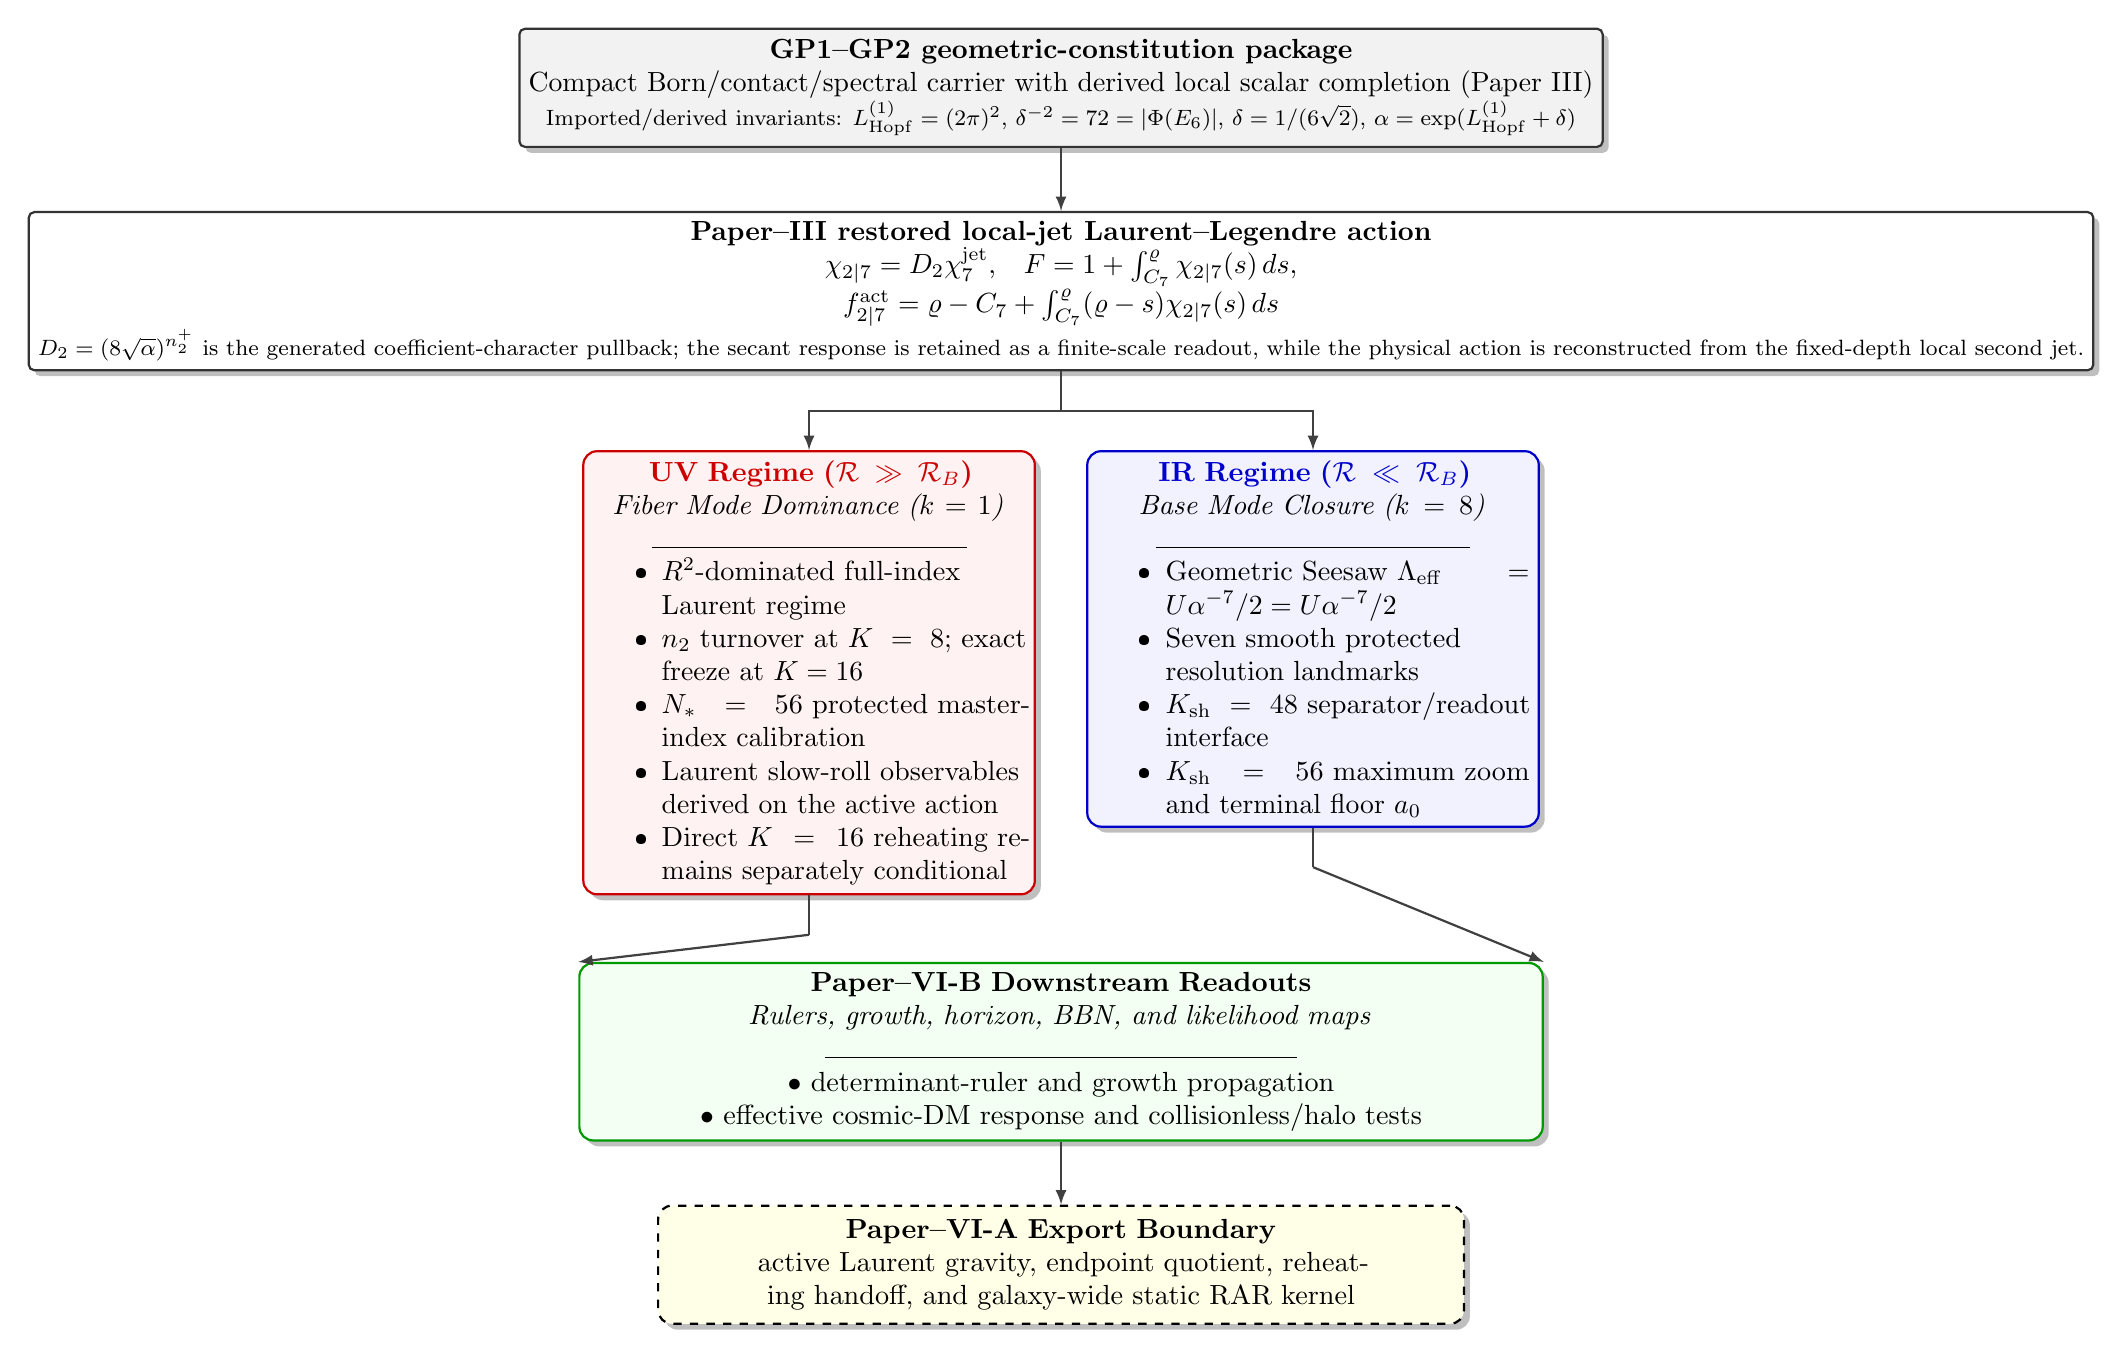
\begin{tikzpicture}[
    node distance=1.5cm,
    axiom/.style={
        rectangle, draw=black!80, thick, fill=gray!10,
        rounded corners=2pt, align=center, minimum height=1.5cm, minimum width=10cm,
        drop shadow
    },
    theory/.style={
        rectangle, draw=black!80, thick, fill=white,
        rounded corners=2pt, align=center, minimum height=1.5cm, minimum width=8cm,
        drop shadow
    },
    uv_regime/.style={
        rectangle, draw=red!80!black, thick, fill=red!5,
        rounded corners=5pt, align=center, text width=5.5cm, minimum height=4.5cm,
        drop shadow
    },
    ir_regime/.style={
        rectangle, draw=blue!80!black, thick, fill=blue!5,
        rounded corners=5pt, align=center, text width=5.5cm, minimum height=4.5cm,
        drop shadow
    },
    resolution/.style={
        rectangle, draw=green!60!black, thick, fill=green!5,
        rounded corners=5pt, align=center, text width=12cm, minimum height=2cm,
        drop shadow
    },
    prediction/.style={
        rectangle, draw=black, dashed, thick, fill=yellow!10,
        rounded corners=5pt, align=center, text width=10cm, minimum height=1.5cm,
        drop shadow
    },
    arrow/.style={-latex, thick, darkgray},
    line/.style={thick, darkgray}
]

\node[axiom] (axiom) {
    \textbf{GP1--GP2 geometric-constitution package} \\
    Compact Born/contact/spectral carrier with derived local scalar completion (Paper~III) \\
    \footnotesize Imported/derived invariants: $L_{\mathrm{Hopf}}^{(1)}=(2\pi)^2$, $\delta^{-2}=72=|\Phi(E_6)|$, $\delta = 1/(6\sqrt{2})$, $\alpha = \exp(L_{\mathrm{Hopf}}^{(1)}+\delta)$
};

\node[theory, below=0.8cm of axiom] (lagrangian) {
    \textbf{Paper--III restored local-jet Laurent--Legendre action} \\
    $\chi_{2\mid7}=D_2\chi_7^{\rm jet}$,\quad
    $F=1+\int_{C_7}^{\varrho}\chi_{2\mid7}(s)\,ds$, \\
    $f_{2\mid7}^{\rm act}=\varrho-C_7+\int_{C_7}^{\varrho}(\varrho-s)\chi_{2\mid7}(s)\,ds$ \\
    \footnotesize $D_2=(8\sqrt\alpha)^{n_2^+}$ is the generated coefficient-character pullback; the secant response is retained as a finite-scale readout, while the physical action is reconstructed from the fixed-depth local second jet.
};

\node[uv_regime, below=1.0cm of lagrangian.south, xshift=-3.2cm] (uv) {
    \textbf{\textcolor{red!80!black}{UV Regime ($\scal \gg \scal_B$)}}\\
    \textit{Fiber Mode Dominance ($k=1$)}\\
    \rule{4cm}{0.4pt} \\
    \begin{itemize}
        \item $R^2$-dominated full-index Laurent regime
        \item $n_2$ turnover at $K=8$; exact freeze at $K=16$
        \item $N_*=56$ protected master-index calibration
        \item Laurent slow-roll observables derived on the active action
        \item Direct $K=16$ reheating remains separately conditional
    \end{itemize}
};

\node[ir_regime, below=1.0cm of lagrangian.south, xshift=3.2cm] (ir) {
    \textbf{\textcolor{blue!80!black}{IR Regime ($\scal \ll \scal_B$)}}\\
    \textit{Base Mode Closure ($k=8$)}\\
    \rule{4cm}{0.4pt} \\
    \begin{itemize}
        \item Geometric Seesaw $\CosmoEff = U\alpha^{-7}/2=U\alpha^{-7}/2$
        \item Seven smooth protected resolution landmarks
        \item $\Ksh=48$ separator/readout interface
        \item $\Ksh=56$ maximum zoom and terminal floor $a_0$
    \end{itemize}
};

\node[resolution, below=7.5cm of lagrangian] (tensions) {
    \textbf{Paper--VI-B Downstream Readouts}\\
    \textit{Rulers, growth, horizon, BBN, and likelihood maps}\\
    \rule{6cm}{0.4pt} \\
    $\bullet$ determinant-ruler and growth propagation \\
    $\bullet$ effective cosmic-DM response and collisionless/halo tests
};

\node[prediction, below=0.8cm of tensions] (predict) {
    \textbf{Paper--VI-A Export Boundary}\\
    active Laurent gravity, endpoint quotient, reheating handoff, and galaxy-wide static RAR kernel
};

\draw[arrow] (axiom) -- (lagrangian);
\draw[line] (lagrangian.south) -- ++(0,-0.5) coordinate (split);
\draw[arrow] (split) -| (uv.north);
\draw[arrow] (split) -| (ir.north);

\draw[line] (uv.south) -- ++(0,-0.5) coordinate (join_uv);
\draw[line] (ir.south) -- ++(0,-0.5) coordinate (join_ir);
\draw[arrow] (join_uv) -- (tensions.north west);
\draw[arrow] (join_ir) -- (tensions.north east);

\draw[arrow] (tensions) -- (predict);

\end{tikzpicture}%
}
\caption{The Logic Flow of Hopf $f(\scal)$ Cosmology. The flowchart illustrates how the GP-constituted geometric sector, completed by the derived scalar pair of Paper~III, splits into distinct high- and low-energy behaviors before recombining into correlated late-time signatures and observable interfaces.}
\label{p8:fig:flowchart-improved}
\end{figure}


Paper~I-A~\cite{Kugelmann2026a} supplies the Hurwitz-link finite carrier, while Paper~III supplies the GP1--GP2 constitution package and the scalar/Lorentzian closure.  Their composition fixes the compact Born/contact/spectral carrier with local Darboux--Born Hamiltonian charts.  Paper~VI-A imports the resulting reduced action and solves its cosmological reductions.

While the compact Born/contact carrier supplies structural stability in spacetime (e.g., filaments), the one-parameter running used below is not an independent flow postulate.  Paper~III derives the common-rate semigroup by an explicit witness-transport constructor from the orbit-invariant scalar split; the uninserted spectral-action class $\Dcl$ controls action-profile insertions but does not generate the determinant finite part.  Separately, the Hopf/contact sector enforces 8-mode Clifford closure, the harmonic trace-response spectrum $\theta_k = 8/k$ (Theorem~\ref{p3:thm:eight-mode-harmonic-response}), and the primitive Hopf contact determinant residue $L_{\mathrm{Hopf}}^{(1)}=(2\pi)^2$.  The value $\delta_0 = 1/(6\sqrt{2})$ is the reduced zeta-determinant shell completion on the declared source scheme $\mathrm{REG}_0$, with the local heat coefficient serving only as an independent consistency check.  Together these give the source hierarchy step
\[
\alpha = \exp(L_{\mathrm{Hopf}}^{(1)} + \delta) \approx 1.57 \times 10^{17}.
\]
 The number $L_{\mathrm{Hopf}}^{(1)}$ is not used here as any global symplectic invariant of $(S^3\times S^1)^2$; it is the Chern--Weil/contact residue of one primitive Hopf threshold, providing the bridge to the dynamical scale.

Notably, this framework has a quantum origin.  The vacuum action prefactor is
\(\hbar c/8\).  On the retained terminal-normalized branch Paper~III-F now
exports the Laurent--Legendre metric coefficient
\begin{equation}
\label{p8:eq:Lagrangian}
 S_{\rm act}=\int d^4x\sqrt{-g}\,\frac{\hbar c}{8}U\,
 f_{2\mid7}^{\rm act}(\varrho),
 \qquad \varrho\ge C_{56},
\end{equation}
with
\[
 D_2(\varrho)=Q^{n_2^+(\varrho)},\qquad Q=8\sqrt\alpha,
\]
\[
 \chi_7^{\rm jet}(\varrho)
 =\frac{(1+n_7^+(\varrho))(\varrho^2-C_{56}^2)}
 {(U+C_{56})\varrho^2},\qquad
 \chi_{2\mid7}(\varrho)=D_2(\varrho)\chi_7^{\rm jet}(\varrho),
\]
and the terminal-normalized same-action reconstruction
\[
 F_{2\mid7}(\varrho)=1+\int_{C_{56}}^{\varrho}\chi_{2\mid7}(s)\,ds,
\]
\[
 f_{2\mid7}^{\rm act}(\varrho)
 =\varrho-C_{56}
  +\int_{C_{56}}^{\varrho}(\varrho-s)\chi_{2\mid7}(s)\,ds.
\]
The exact reciprocal Laurent curve
$\mathscr H_7^{\rm sec}=(\varrho^2+UC_{56})/(U+C_{56})$ remains a finite-scale
secant readout; it is not differentiated as the physical local metric Hessian.
After the Einstein--Hilbert normalization is factored out, the active
Jordan-frame metric function is therefore
\begin{equation}
\label{p8:eq:fstd-normalized}
 \boxed{f_{\rm std}(\varrho)=f_{2\mid7}^{\rm act}(\varrho).}
\end{equation}
The terminal zero-order intercept is the same-action Clifford
scalar-remnant contribution \(-C_{56}\); there is no independent
\(\mathrm{TERMREN}_7\) datum and no additional subtraction on top of the
inverse-Euler action.
The former copied-response expression
\(\varrho+D_2\mathcal H_7^{\rm act}-2C_{56}\) remains only a historical
diagnostic.  The current action separates the generated positive response
from its same-action Legendre primitive; there is no \(S(n)\).

At terminal resolution the positive response has attained the hierarchy magnitude
\(P_{2\mid7}(C_{56})=C_{56}=\mathcal R_{56}^2\), while the reconstructed
action has value zero and slope one.  On the retained terminal-normalized branch the later Einstein coefficient is therefore
\begin{equation}
 f_{\rm term}(R_{\rm g})=R_{\rm g}-C_{56}
 =R_{\rm g}-2\CosmoEff.
\end{equation}
The structural response readout \(U C_{56}=U^2\alpha^{-7}\) remains valuewise
fixed and is not a second freely varied Einstein--Hilbert term.  In Planck/Newton coordinates this is
\(U C_{56}=U^2\alpha^{-7}\).  The active
resolution coordinate \(\varrho\) agrees with the FLRW Ricci scalar before
the endpoint; afterward the separately typed curvature \(R_{\rm g}\) remains
dynamical.  A physical handoff still requires an actual history.  No independent
microscopic smoothing/profile/width datum is required or licensed by the
mathematical action.

% BEGIN MINIMAL COMPLETE COSMOLOGICAL ACTION v2.171 / framework v2.198
% Source Paper VI-A, original line 17612
\subsection{Reproducibility Snippets}
% Source Paper VI-A, original line 17613
\subsubsection{Pivot calibration and optional fixed-rank arithmetic}
\begin{verbatim}
import sympy as sp

# N_* is an explicit pivot calibration in Paper VI-A,
# not derived from H8.
N_star = 56

# Fixed-rank response values are native theorem outputs.
theta = {k: sp.Rational(8, k) for k in range(1, 9)}

# H8 is only an optional arithmetic mean ingredient if one independently
# declares the uniform rank measure mu_k = 1/8.
H8 = sum(sp.Rational(1, k) for k in range(1, 9))
assert H8 == sp.Rational(761, 280)
\end{verbatim}

% Source Paper VI-A, original line 17629
\subsubsection{Numerical implementation for the shell-resolved RAR response}
\label{p8:app:darkmatter}

The reduced implementation should use the static acceleration readout and the hierarchy-selected Reeb kernel, not a fixed scalaron mass iteration.  The following minimal code computes the terminal \(j=56\) response, the projected hierarchy endpoints, and the selected Reeb/RAR response for a supplied uplift factor \(\Lambda\).

\begin{lstlisting}[
language=Python,
basicstyle=\ttfamily\footnotesize,
frame=single,
xleftmargin=0pt,
xrightmargin=0pt,
framesep=2pt,
framerule=0.3pt,
breaklines=true,
breakatwhitespace=true,
columns=fullflexible,
keepspaces=true
]
import numpy as np
from scipy.constants import c, hbar, G, pi

# Geometric constants
delta_star = 1.0 / (6.0 * np.sqrt(2.0))
alpha = np.exp((2.0 * np.pi)**2 + delta_star)
Rp = c**3 / (2.0 * np.pi * hbar * G)      # Paper V-C convention
kappa_U = 1.0  # Paper III-E generated-branch calibration
C56 = kappa_U * Rp * alpha**(-7.0)
a56 = (c**2 / (4.0 * np.pi)) * np.sqrt(C56)

def R_from_g(g):
    """Acceleration-to-curvature representative, SI units."""
    return (4.0 * np.pi * g / c**2)**2

def Lambda_endpoint(s):
    """Projected Hopf-charge endpoint Lambda_s = alpha^(s/16)/(s+1)."""
    return alpha**(s / 16.0) / (s + 1.0)

def Lambda_between(s, eta):
    """Logarithmic interpolation between adjacent projected endpoints."""
    return Lambda_endpoint(s)**(1.0 - eta) * Lambda_endpoint(s + 1)**eta

def nu_reeb(y):
    """Closed Reeb-return kernel."""
    return 1.0 / (1.0 - np.exp(-np.sqrt(y)))

def g_response(gb, Lambda=1.0):
    """Hierarchy-selected static response."""
    a_star = Lambda * a56
    return nu_reeb(gb / a_star) * gb

def g_deep_response(gb, Lambda=1.0):
    """Deep-side asymptotic of the selected sector."""
    return np.sqrt(Lambda * a56 * gb)
\end{lstlisting}

\paragraph{Superseded historical RAR diagnostic.}
The following table is retained only to identify the former comparison
calculation.  Release v1.64 proves that its one-sided interpolation kernel is
not the Hessian response of the occurring metric action; it is therefore not
an active prediction.
\[
\begin{array}{c|c|c|c}
R\;({\rm kpc}) & v_b\;({\rm km\,s^{-1}}) & v_{\rm RAR}\;({\rm km\,s^{-1}}) & g_b/a_0\\
\hline
5.0 & 190 & 218 & 2.0\\
8.2 & 179 & 222 & 1.1\\
12.0 & 157 & 215 & 0.58\\
20.0 & 122 & 201 & 0.21\\
25.0 & 108 & 196 & 0.13
\end{array}
\]
This table neither verifies the action mechanism nor supplies a physical fit.
The function \texttt{nu\_reeb} evaluates the separately declared Reeb-return
kernel, not the same-action metric Green function.  It may be used only as an
enlarged comparison branch.

% Source Paper VI-A, original line 17705
\subsubsection{RAR Acceleration Parameter}
\textbf{Verification with SymPy:}
\begin{verbatim}
import sympy as sp

c, Lambda_eff = sp.symbols('c Lambda_eff', positive=True)
a_0 = c**2 * sp.sqrt(2 * Lambda_eff) / (4 * sp.pi)

Lambda_prim_num = 1.2835e-52
a_0_prim_num = (
    (299792458**2) * sp.sqrt(2 * Lambda_prim_num)
    / (4 * sp.pi)
)
# 1.146e-10 m/s^2 on the primitive-curvature metrological realization
\end{verbatim}
This evaluates the hierarchy number
$a_{56}\simeq1.146\times10^{-10}\,\mathrm{m/s^2}$ in the displayed unit
convention; it does not verify a generated local force law.
The DtN eigenvalue itself remains $\mathcal N_R1=\sqrt R$;
$4\pi$ enters only when the total isotropic contact-flux trace is converted to
the unique $SU(2)$-invariant local solid-angle density.

The historical local-metric comparator has the terminal Einstein response
in Theorem~\ref{p8:thm:v164-static-metric-response} below; that comparator
is not a replacement for the complete native deep $S+T$ response.

% Source Paper VI-A, original line 18995
\subsection{Expansion-aware reciprocal-position diagnostics}
\label{p8:app:v191-expansion-reciprocal-diagnostics}

% Source Paper VI-A, original line 18998
\subsubsection{Position-side reciprocal $2I$ compatibility filtration}
Let $P_m^x$ denote the complete position-band projector and let
$\Pi_{2I}^x$ be the group-average projector of the generated reciprocal
position action.  Because both commute with the round scalar Laplacian,
\[
 [P_m^x,\Pi_{2I}^x]=0.
\]
Writing
\[
 M_{2I}(t)=\sum_{k\ge0}\mu_k^{2I}t^k,
\]
the compatible position-space rank is
\[
 \dim\bigl(\mathcal P_x(m)\cap\operatorname{Ran}\Pi_{2I}^x\bigr)
 =\sum_{k=0}^m(k+1)\mu_k^{2I}.
\]
Hence the nonconstant rank is zero through $m=11$ and first jumps to $13$ at
$m=12$.  Including the constant gives total rank $14$ there.  This is
representation mathematics only: physical position is not quotiented by
$2I$.  The cross-role harmonic carrier bridge is source-closed by
Theorem~\ref{p8:thm:g30a-2i-mukhanov-bridge}; the primordial initial-state/complex-structure role is G30b and does not follow from representation transport alone.  On the native cyclic lineage that role is now closed by Theorem~\ref{p8:thm:v2114-fresh-root-neutral-qroot}; Corollary~\ref{p8:cor:v245-deterministic-covariance-transport} then generates the subsequent linear covariance.  On the cyclic lineage the
background is \(h_{\rm cyc}\), subject to its continuation/reach certificate,
not an independent G30b history token.

% Source Paper VI-A, original line 19022
\subsubsection{Observable-order finite-support detectability}
Uniform $2I$ evaluation is exact through total polynomial degree eleven.
Therefore an $r$-field local polynomial observable built from
$\mathcal P_x(m)$ is guaranteed blind whenever $rm\le11$.  Since products
of degree-at-most-$m$ coordinate polynomials span the degree-at-most-$rm$
polynomial restrictions, the nonzero degree-twelve defect functional can
first be reached at
\[
 m=3\ \text{(quartic)},\qquad
 m=4\ \text{(cubic)},\qquad
 m=6\ \text{(quadratic)},\qquad
 m=12\ \text{(linear)}.
\]
These are first-possible finite-support detectability thresholds, not one
common cosmological cutoff.  The quartic $m=3$ threshold is independently
witnessed by the explicit degree-twelve defect already recorded for
$f=x_0^3$.

% Source Paper VI-A, original line 19040
\subsubsection{Occurrence-axis/Borel--Weil candidate and remaining state firewall}
A noncentral relative occurrence $q=ab^{-1}$ determines a Born-even
unoriented maximal-torus axis.  Within any independently identified observer
$SU(2)$ carrier, Borel--Weil sends that axis to the extremal pair
$\operatorname{span}\{|\ell,+\ell\rangle,|\ell,-\ell\rangle\}$.
Two physical arrows remain open: the relative axis must be mapped to the
observer-sky rotation axis, and the mathematical extremal-pair projector must
be actualized as the primordial state/covariance support.  Consequently the
main-text planar Born--Hopf branch remains conditional.

% Source Paper VI-A, original line 19050
\subsubsection{Rejected horizontal-Casimir route}
The isotropic scalar Hessian cannot be replaced by a Hopf-horizontal
sub-Laplacian merely because an occurrence supplies an axis.  Moreover the
Hopf vertical charge and the observer magnetic quantum number are differently
typed operators in the current framework.  The horizontal-Casimir argument
therefore does not derive CMB planarity and is excluded from the positive
proof chain.



% BEGIN V202 TRACE JUNCTION SCOPE
% Source Paper VI-A, original line 19061
\subsubsection{Trace continuity across the Legendre coefficient freeze}
\label{p8:app:v202-trace-junction}
For the reconstructed action, \(f\) and \(f_R\) are continuous at \(C_2\), so
the trace map is also continuous:
\begin{equation}
\label{p8:eq:v202-trace-junction-jump}
 \boxed{\mathcal T(C_2^+)-\mathcal T(C_2^-)=0.}
\end{equation}
Its derivative \(N=f_R-Rf_{RR}\) has a finite one-sided step because
\(f_{RR}\) does.  The uniform positivity theorem gives \(N>0\) on both
sides, so \(\mathcal T\) is strictly increasing through the junction as a
continuous map.  Therefore the former two-stratum source overlap caused by a
finite trace jump is retired on the Legendre branch.  This statement is about
the mathematical action; a finite-duration physical transition/history is
still separate occurrence data.
% END V202 TRACE JUNCTION SCOPE

% Source Paper VI-B, original line 4317
\subsection{Historical G26 readout synchronization prior to the v1.92 operator closure}
\label{p9:sec:v192-g26-readout-sync}

\begin{theorem}[Historical one-sided/global G26 readout frontier after the source-stiffness repair]
\label{p9:thm:v192-g26-readout-frontier}
The active local structural chain is
\[
 B_{48}
 \xrightarrow{\text{parent collar / PCAD}}
 J_\partial
 \xrightarrow{\text{same-action Schur}}
 K_\partial
 \xrightarrow{\beta_{48}^{*}(\cdot)\beta_{48}}
 K_{48}.
\]
The first arrow is generated on the regular local branch and is no longer a
G26 premise.  On the promoted scalar line write the computed same-action
stiffness as \(\lambda(y)\), \(y=g_b/a_*\).  Paper~VI-A now separates the
three downstream operations:
\[
 \lambda(y)
 \longmapsto
 \sqrt{\lambda(y)}
 \longmapsto
 e^{-\sqrt{\lambda(y)}}
 \longmapsto
 \frac{1}{1-e^{-\sqrt{\lambda(y)}}}.
\]
Conditional identification of the Born-balanced terminal deep projection with
this same occurring static response fixes only
\[
 \lambda(0)=0,\qquad \lambda'(0)=1
\]
under differentiability, and hence the leading
\(\sqrt y+O(y^{3/2})\) critical law under the stated regularity.  Exact
all-order \(\lambda(y)=y\) still requires (R1) or an equivalent exact-action
source-composition theorem; the one-sided return class still requires (R2);
and the physical occurrence of the unbounded collar/return limit remains a
separate refinement/history obligation.  The mathematical finite-collar
operator limit itself is controlled with uniform absolute \(O(L^{-1})\)
error, while the normalized critical ratio is nonuniform at \(y=0\).

Therefore the minimal local \(f(R)\) branch still does not export the
historical exact one-sided/global RAR envelope.  The v1.87 local owner closure
narrows that stronger Reeb/one-sided boundary route.  The later Release~v1.92
operator theorem retires this route as a core native closure requirement; its
source-law, return-ownership and physical unbounded-limit conditions survive
only for the optional elementary comparison branch.
\end{theorem}

\begingroup
\small
\RaggedRight
\hyphenpenalty=300
\exhyphenpenalty=300
\emergencystretch=8em
\sloppy
% \printbibliography relocated to the end of the active volume
\endgroup

% Source Paper VI-B, original line 4377
\subsection{downstream synchronization of K16, K48, and the closed deep RAR law}
\label{p9:sec:v173-downstream-k16-k48-rar-sync}

The generic source-free $K=16$ crossing consumes the upstream generalized
flux law
\[
 \boxed{\chi_+\dot R_+=\chi_-\dot R_-}
\]
in homogeneous notation.  A zero crossing rate is retained only on the
additional $C^1$-curvature branch.  The action fixes the deterministic symplectic/Bogoliubov map once the
applicable background and initial complex structure/covariance are supplied.
On the cyclic lineage the background is generated from the complete-cap root,
subject to \(\mathrm{PROP}^{\rm cyc}_{16}\); produced occupation,
backreaction and thermalization remain state/history functionals rather than
free transfer laws.

At the terminal corridor, $K=48$ is the midpoint/realization bifurcation of the
full $q=5\to7$ depletion and the onset of the final primitive subtransfer.  The
neutral current package
\[
 Q_D,\quad J_D=Q_D\Omega_H,\quad
 \pi_!J_D=Q_D\frac{d\Omega}{4\pi},\quad
 \widehat\zeta_D=\frac{Q_D}{2\pi^2a^3}
\]
is denoted $\mathrm{K48GEOM}$ and is structurally closed.  Framework v2.92
supersedes the historical separate-owner typing: the native physical cDM stress
owner is the co-realized homogeneous $H$-modality curvature response of the
same metric-$f(R)$ action.  On a generic branch the cold history remains a
history input; on the cyclic lineage it is a predicate on the generated
history, conditional on \(\mathrm{PROP}^{\rm cyc}_{48}\).  Present-slice
selection and numerical abundance remain downstream readouts.  A separately conserved material-current energy ledger,
for which one may write
\[
 M_D(q)=\int_0^q\varepsilon(s)\,ds,
\]
is an optional stronger comparison rather than the native $K=48$ owner.

The controlling G26/RAR status is now
\[
 \boxed{\mathrm{G26\!\! -\! DEEP}:\ \text{closed}},
 \qquad
 \boxed{\mathrm{ENVRESP}_{\rm fixed}:\ \text{closed analytic operator}}.
\]
The closed terminal law imported from Paper~VI-A is
\[
 \boxed{g_{\rm obs}^2=a_0g_b,
 \qquad a_0=\frac{c^2}{4\pi}\sqrt{C_{56}}},
\]
equivalently $x^2=y$ and
$\mathcal P_{\rm IR}(z)=2z^{3/2}/3$ for the effective terminal $S+T$ response.
This does not turn the local metric modality into the RAR modality.  The
Newton-to-deep endpoints still do not select a unique elementary scalar
interpolation, but Paper~VI-A Release~v2.123 shows that none is required: the
complete fixed-environment law is the generated source-conditioned Schur
operator.  A closed-form Reeb interpolation is an optional stronger reduction.

The I-A/I-B Gaussian boundary calculus remains available as supporting exact
boundary mathematics; its possible stronger physical owner is not a condition
for the above deep law.  Likewise $Q_D$ is neither $x$ nor $y$, and the cDM
current, static RAR response and coherent scalaron histories remain distinct
physical descendants.

On the optional separately conserved material-current branch, if
$\mathrm{K48MATERIAL}+\mathrm{K48MATCH}$ is derived, the resulting material
cDM charge contributes
\[
 D_{\rm cDM}=\rho_{\rm cDM}a^3,
 \qquad
 \mathfrak M_{\rm cDM}=\frac{\kappa D_{\rm cDM}\sqrt\Lambda}{2}
\]
to the Paper--VI-A closed-FLRW fate discriminant.  Present-slice abundance,
actual total dust charge and turnaround scalaron momentum remain history/readout
data.


% Source Paper VI-B, original line 4487
\subsection{retirement of the H8 lithium normalization}
\label{p9:sec:v184-h8-retirement}
The K=40 thermal placement remains available as a diagnostic coordinate.  The former static light-quark construction from
\(H_8\) and the resulting \(1/H_8\) lithium kernel are withdrawn from the
native dependency graph.  A quantitative lithium prediction is stale until
\(M_q^{\rm phys}(\mu)\) is propagated through a controlled QCD/chiral/nuclear
matching and the mass-seven network response.  No alternative numerical mass
selector is assumed in this release.
% END SAFEGUARD-LITHIUM-H8-RETIREMENT v1.84


% BEGIN N7-LOCAL-JET RESTORATION v1.86
% Source Paper VI-B, original line 4499
\subsection*{K16 after rank-seven local-jet restoration}
The restored result is deliberately split:
\[
 \boxed{\mathrm{RAPID16}_{\rm cyc}=\texttt{CLOSED\_ANALYTIC}},\qquad
 \boxed{\mathrm{RUNMASS16}_{\rm entry}=\texttt{CLOSED\_ANALYTIC}},
\]
\[
 \boxed{\mathrm{NARROW16}_{\rm cyc}
 =\texttt{CLOSED\_DEPENDENT[PERTURBATIVE\ RG]}}.
\]
Actual occupation consumes the now-generated cyclic root state, while physical RG/matching
still fixes the couplings, and the duration of the backreacted production era
is an output of the coupled evolution.  None of these remaining typed inputs
is a free damping parameter.
% END N7-LOCAL-JET RESTORATION v1.86

% BEGIN POST-N7 DOWNSTREAM CLOSURE v1.87


\printbibliography


% BEGIN FRAMEWORK v2.353: BOUNDARY-SCHUR ACTION DISCHARGE LEDGER
\section{Cap boundary-Schur and native-action discharge ledger}
\label{p6c:sec:v353-native-cap-ledger}
The exact finite mathematical results new in the v2.353 addition are:
(i) the positive half-boost identity for the inherited cap profile,
(ii) the $2+2$ Schur source-return formula and its reference Hessian
jet, (iii) the conditional Clifford-projector transversality
criterion, and (iv) the interior grading-parity obstruction to the
\emph{direct} odd-scalar identification.  They do not modify the
capped scalar working density or turn any conditional comparison
into a microscopic-action or physical-history theorem.

\begin{proposition}[Finite scalar source equivalence does not close the action]
\label{p6c:prop:v353-native-action-status}
For $S_+>0$ with $\dim_{\mathbb C}E_+=2$, the scalar cap identity is
\[
 \operatorname{Tr}_{E_+}(S_+^{-2})=2/b(R)^2,
 \qquad b(R)=B(R)/B_I.
\]
It does not imply $S_+=bI_2$ without a licensed scalarity/rotation
premise; nor does $S_+=bI_2$ imply full source, tensor or boundary
action identity.  The stronger native operator target is the actual
same-owner transported $S_+^{\rm native}=bI_2$ and the reduced
physical source two-jet of
Proposition~\ref{p3f:prop:v353-observable-quadratic}, together with
the tensor test of Proposition~\ref{p3f:prop:v289-flrw-tensor-obstruction}.
\end{proposition}
\begin{proof}
The strict counterfamily $S_\varepsilon$ of
Proposition~\ref{p3e:prop:v353-schur-orientation} has the scalar
trace identity but is non-scalar for $\varepsilon\ne0$.  Distinct
unitary orientations give identical scalar returns but different
mixed boundary responses.  The pure $f(R)$ and Weyl-squared
comparison of Paper~III-F has identical FLRW restrictions but
different tensor Hessians.
\end{proof}

\paragraph{Explicit open discharges (not GP2 insertions).}
The following remain physical same-action certificates rather than
additional axioms: the actual boundary/source incidence and covariant
transport; the conormal amplitude $b_\partial^2\gamma_N^2d_0=4\Delta$
(where $b_\partial$ is the boundary amplitude, not the cap ratio
$b=B/B_I$); finite/internal multiplicity and density weight; the
mode-dependent Dirichlet-to-Neumann reduction; native tensor and
Hilbert source matching; and the actual cosmological initial/transfer
history.  The first two native curvature-jet requirements are
Eq.~\eqref{p3e:eq:v353-native-jet-target} and are \emph{tests}, not
verified equalities.  The Kneser/Petersen and foundational
operator-reconstruction overlays of v2.352 retain their separate
status.
% END FRAMEWORK v2.353


% BEGIN FRAMEWORK v2.358: observer-window and optical counterchecks (DAG v1.20-v1.21)
\section{Windowing, source covariance and optical countermodels}
\label{p6c:sec:v358-window-optical-technical}
\begin{proposition}[Noncommutation of finite smoothing and kinematic null]
\label{p6c:prop:v358-window-null-contamination}
For the comparison polynomial
$F(y)=A_0+A_2y^2+A_3y^3+A_4y^4$ and an equal-half-width
symmetric top-hat averaging operator
$\mathcal W_hF(y)=(2h)^{-1}\int_{y-h}^{y+h}F(t)\,dt$,
let
$\mathscr D[F]:=F'-yF''+\frac12y^2F'''$.  Then
\[
 \mathscr D[F]=4A_4y^3,\qquad
 \mathscr D[\mathcal W_hF]=4A_4y^3+A_3h^2.
\]
In particular on the dust--curvature--vacuum comparison subbranch
$A_4=0$, the pointwise null vanishes while
$\mathscr D[\mathcal W_hF]=A_3h^2$.  Thus applying a pointwise
kinematic null to an averaged history can create an apparent extra
signal even on an exact comparison history.
\end{proposition}
\begin{proof}
Direct integration gives
\[
 \mathcal W_hF=A_0+A_2(y^2+h^2/3)
 +A_3(y^3+yh^2)+A_4(y^4+2y^2h^2+h^4/5).
\]
Differentiation yields the two displayed identities.  The exact
measurement map is an extra assumption; the autonomous source
pushforward need not equal this convolution.
\end{proof}

\begin{proposition}[Mean-square and nonlinear observational readout]
\label{p6c:prop:v358-mean-square-window}
For a normalized positive window $W$ and a square-integrable
expansion function $H$,
\[
 \int H^2\,dW=\left(\int H\,dW\right)^2
   +\operatorname{Var}_W(H).
\]
If $H$ is $L$-Lipschitz on the window support,
$0\le\operatorname{Var}_W(H)\le L^2\operatorname{Var}_W(y)$.
Hence the protocol averaging $H^2$ cannot silently be replaced by
the square of a survey average of $H$.
\end{proposition}
\begin{proof}
The first identity is the variance definition.  For independent
$Y,Y'$ distributed under $W$,
$\operatorname{Var}(H(Y))=\frac12\mathbb E
|H(Y)-H(Y')|^2\le\frac12L^2\mathbb E|Y-Y'|^2
=L^2\operatorname{Var}(Y)$.
\end{proof}

\begin{proposition}[Positive optical-speed nonidentifiability]
\label{p6c:prop:v358-optical-speed-counterfamily}
Let $H(z)>0$ and a differentiable transverse-distance function
$D(z)>0$ with $D'(z)>0$ be fixed on an interval, with calibrated
operational $c>0$.  For every candidate closed spatial curvature
$K>0$ satisfying $KD(z)^2<1$, set
\[
 g_K(z)=\frac{H(z)D'(z)}{c\sqrt{1-KD(z)^2}}>0.
\]
Then the optical transport equation
$(HD'/c)^2=g_K(z)^2(1-KD^2)$ is satisfied by the \emph{same}
$H,D$ for every such $K$.  Thus positive closed spatial curvature
cannot be uniquely reconstructed from $(H,D)$ alone if an independent
optical-speed degree of freedom is allowed.  This formal counterfamily
is not asserted to be the Born--Hopf photon dynamics.
\end{proposition}
\begin{proof}
Substitution is an identity.  Two distinct admissible positive
curvatures have different $g_K$ while producing identical data.
The metric optical assumption sets $g_K\equiv1$ and removes this
constructed degeneracy; its physical validity must therefore come
from the same-action photon source and detector transfer.
\end{proof}

\begin{remark}[Observer and clock remain relational inputs]
\label{p6c:rem:v358-observer-clock-frontier}
Paper~VI-B's measurement/rank and curvature tests depend on a known
calibrated window, clock/redshift map and photon propagation law.
The formulas in this technical section neither select an occurring
cosmological observer nor strengthen the native photon cone theorem
beyond its declared stationary Yang--Mills branch.
\end{remark}
% END FRAMEWORK v2.358


\paragraph{Reference-action Hilbert-source clarification (v3.053).}
On the adopted Paper~III-F reference branch, the Hilbert tensor on the
right-hand side of the metric Euler equation is the metric variation
of the independently varied material functional in the declared split.
Varying the \emph{entire} action gives the full Euler derivative, zero
on shell; it is not a separately normalized matter stress source.
The reference pullback and nonminimal terms must be varied exactly once.
This is a conditional same-action source convention, not a proof of an
unconditional physical matter background.

\end{document}
